%%%%%%%%%%%%%%%%%%%%%%%%%%%%%%%%%%%%%%%%%
% Masters/Doctoral Thesis 
% LaTeX Template
% Version 1.43 (17/5/14)
%
% This template has been downloaded from:
% http://www.LaTeXTemplates.com
%
% Original authors:
% Steven Gunn 
% http://users.ecs.soton.ac.uk/srg/softwaretools/document/templates/
% and
% Sunil Patel
% http://www.sunilpatel.co.uk/thesis-template/
%
% License:
% CC BY-NC-SA 3.0 (http://creativecommons.org/licenses/by-nc-sa/3.0/)
%
% Note:
% Make sure to edit document variables in the Thesis.cls file
%
%%%%%%%%%%%%%%%%%%%%%%%%%%%%%%%%%%%%%%%%%

%----------------------------------------------------------------------------------------
%	PACKAGES AND OTHER DOCUMENT CONFIGURATIONS
%----------------------------------------------------------------------------------------

\documentclass[11pt, oneside]{Thesis} % The default font size and one-sided printing (no margin offsets)
\usepackage{xcolor}
\hypersetup{
    colorlinks,
    linkcolor={black},
    citecolor={black},
    urlcolor={black}
}
\graphicspath{{Pictures/}} % Specifies the directory where pictures are stored

\setcounter{tocdepth}{1}
%--------------------------------------------------------------------------------------------
%PACKAGES
%-----------------------------------------------------------------------------------------------
\usepackage{multicol}
\usepackage[square, comma, sort&compress]{natbib} % Use the natbib reference package - read up on this to edit the reference style; if you want text (e.g. Smith et al., 2012) for the in-text references (instead of numbers), remove 'numbers' 
\hypersetup{urlcolor=blue, colorlinks=true} % Colors hyperlinks in blue - change to black if annoying
\title{\ttitle} % Defines the thesis title - don't touch this

\makeatletter
\renewcommand\subsubsection{\@startsection{subsubsection}{3}{\z@}%
                                     {-3.25ex\@plus -1ex \@minus -.2ex}%
                                     {-1.5ex \@plus -.2ex}% Formerly 1.5ex \@plus .2ex
                                     {\normalfont\normalsize\bfseries}}
\makeatother
\usepackage{verbatim}
\usepackage{mathtools}
\usepackage[colorlinks]{hyperref}
\usepackage[acronym,toc]{glossaries}
\usepackage{graphicx}
\usepackage{subcaption}
\usepackage{pdfpages}
\usepackage{epstopdf}
\epstopdfsetup{update} 
\usepackage{fixltx2e}
\usepackage{bm}
\usepackage{pseudocode}
\usepackage{mathtools}
\usepackage{tikz}
\usepackage{pgf}
\usepackage{lmodern}
\usetikzlibrary{arrows,automata}
\usetikzlibrary{positioning}
\usetikzlibrary{shadows,shapes,decorations}
\usepackage{pgfplots}
\pgfplotsset{compat=newest}
\usepackage[all]{xy}
\usetikzlibrary{calc,fit}
\usepackage[colorinlistoftodos]{todonotes}
\usepackage{bbm}
\usepackage{multirow}
\usepackage{alltt}
\usepackage{verbatim}
%%%%%%%%%%%%%%%%%%%%%%%%%%%%%%%%%%%%%%%%%%%%%%%%%%%%%%%%%%%%%%%%%%%%%%%%%%%%%%%%%%%%%%%%%%%%%%%%
% COMMANDS
%%%%%%%%%%%%%%%%%%%%%%%%%%%%%%%%%%%%%%%%%%%%%%%%%%%%%%%%%%%%%%%%%%%%%%%%%%%%%%%%%%%%%%%%%%%%%%%%%%%
\newcommand\independent{\protect\mathpalette{\protect\independenT}{\perp}} \def\independenT#1#2{\mathrel{\rlap{$#1#2$}\mkern2mu{#1#2}}}
\newcommand{\y}{\bm{y}}
\newcommand{\De}{\mathcal{D}}
\newcommand{\dr}{\textnormal{d}}
\newcommand{\E}{\mathbb{E}}
\newcommand{\V}{\mathbb{V}}
\newcommand{\D}{\bm{D}}
\newcommand{\B}{\textnormal{B}}
\newcommand{\Y}{\bm{Y}}
\newcommand{\Gr}{\mathcal{G}}
\newcommand{\pa}{\bm{\theta}}
\newcommand{\Cov}{\mathbb{C}}
\newcommand{\MY}{\mathcal{Y}}
\newcommand{\R}{\bm{R}}
\newcommand{\Do}{\textnormal{do}}
\newcommand{\EU}{\textnormal{EU}}
\newcommand{\N}{\textnormal{N}}
\newcommand{\Multi}{\textnormal{Multi}}
\newcommand{\Be}{\textnormal{Be}}
\newcommand{\Bin}{\textnormal{Bin}}
\newcommand{\NIG}{\textnormal{NIG}}
\newcommand{\Di}{\textnormal{Di}}
\newcommand{\IG}{\textnormal{IG}}
\newcommand{\blockdiag}{\textnormal{blockdiag}}
\newcommand{\diag}{\textnormal{diag}}
\newcommand{\IW}{\textnormal{IW}}
\newcommand{\NIW}{\textnormal{NIW}}
\newcommand{\HIW}{\textnormal{HIW}}
\newcommand{\Exp}{\textnormal{Exp}}
\newcommand{\T}{\textnormal{T}}
\newcommand{\tr}{\textnormal{tr}}
\newcommand{\Rs}{\mathcal{R}}
\newcommand{\ci}[3]{#1\independent #2 \;|\; #3}
\newcommand{\bci}[3]{\lfloor#1\independent #2 \rfloor \;/\; #3}
\newcommand{\UT}{U}
\DeclareMathOperator*{\argmax}{arg\,max}
%-------------------------------------------------------------------------
% COLORS
%------------------------------------------------------------------------
\definecolor{Blau0}{RGB}{0,0,150}
\definecolor{Blau1}{RGB}{25,25,255}
\definecolor{Blau2}{RGB}{0,162,232}
\definecolor{Blau3}{RGB}{175,226,239}
\definecolor{Gruen0}{RGB}{0,150,0}
\definecolor{Gruen1}{RGB}{0,255,0}
\definecolor{Rot0}{RGB}{150,0,0}
\definecolor{Rot1}{RGB}{255,25,25}

%-------------------------------------------------------------------------------------
%GLOSSARY
%-----------------------------------------------------------------------------------
\makeglossaries
\newacronym{DSS}{DSS}{Decision Support System}
\newacronym{ES}{ES}{Expert System}
\newacronym{DM}{DM}{Decision Maker}
\newacronym{MN}{MN}{Markov Network}
\newacronym{BN}{BN}{Bayesian Network}
\newacronym{RODOS}{RODOS}{Real-time On-line DecisiOn Support system}
\newacronym{MCDA}{MCDA}{MultiCriteria Decision Analysis}
\newacronym{ASY}{ASY}{Analsying SubsYstem}
\newacronym{CSY}{CSY}{Countermeasure SubsYstem}
\newacronym{ESY}{ESY}{Evaluating SubsYstem}
\newacronym{UG}{UG}{Undirected Graph}
\newacronym{ID}{ID}{Influence Diagram}
\newacronym{SEU}{SEU}{Subjective Expected Utility}
\newacronym{DAG}{DAG}{Directed Acyclic Graph}
\newacronym{CG}{CG}{Chain Graph}
\newacronym{OOBN}{OOBN}{Object Oriented Bayesian Network}
\newacronym{IDSS}{IDSS}{Integrating Decision Support System}
\newacronym{CEG}{CEG}{Chain Event Graph}
\newacronym{DLM}{DLM}{Dynamic Linear Model}
\newacronym{MDM}{MDM}{Multiregression Dynamic Model}
\newacronym{LMDM}{LMDM}{Linear Multiregression Dynamic Model}
\newacronym{DCG}{DCG}{Dynamic Chain Graph}
\newacronym{DBN}{DBN}{Dynamic Bayesian Network}
\newacronym{2-TBN}{2-TBN}{2-Time-slice Bayesian Network}
\newacronym{GP}{GP}{Gaussian Process}
\newacronym{UI}{UI}{Utility Independent}
\newacronym{CUI}{CUI}{Conditional Utility Independent}
\newacronym{CBN}{CBN}{Causal Bayesian Network}
\newacronym{logOp}{logOp}{logarithmic Opinion pool}
\newacronym{EB}{EB}{Externally Bayesian}
\newacronym{CEB}{CEB}{Conditional External Bayesianity}
\newacronym{PCG}{PCG}{Probabilistic Chain Graph}
\newacronym{GAI}{GAI}{Generalised Additive Independent}
\newacronym{MID}{MID}{Multiplicative Influence Diagram}
\newacronym{DS}{DS}{Decision Sequence}
\newacronym{DDM}{DDM}{Distributed Dynamic Model}
\newacronym{SB}{SB}{SupraBayesian}
\newacronym[plural=CK-classes]{CK-class}{CK-class}{Common Knowledge-class}
\newacronym{rhs}{rhs}{right hand side}
\newacronym{AC}{AC}{Arithmetic Circuit}
\newacronym{SEM}{SEM}{Structural Equation Model}
\newacronym{iff}{iff}{if and only if}


%%%%%%%%%%%%%%%%%%%%%%%%%%%%%%%%%%%%%%%%%%%%%%%%%%%%%%%%%%%%%%%%%
% DOCUMENT
%%%%%%%%%%%%%%%%%%%%%%%%%%%%%%%%%%%%%%%%%%%%%%%%%%%%%%%%%%%%
\begin{document}

\frontmatter % Use roman page numbering style (i, ii, iii, iv...) for the pre-content pages

\setstretch{1.3} % Line spacing of 1.3

% Define the page headers using the FancyHdr package and set up for one-sided printing
\fancyhead{} % Clears all page headers and footers
\rhead{\thepage} % Sets the right side header to show the page number
\lhead{} % Clears the left side page header

\pagestyle{fancy} % Finally, use the "fancy" page style to implement the FancyHdr headers

\newcommand{\HRule}{\rule{\linewidth}{0.5mm}} % New command to make the lines in the title page

% PDF meta-data
\hypersetup{pdftitle={\ttitle}}
\hypersetup{pdfsubject=\subjectname}
\hypersetup{pdfauthor=\authornames}
\hypersetup{pdfkeywords=\keywordnames}

\numberwithin{equation}{section}

%----------------------------------------------------------------------------------------
%	TITLE PAGE
%----------------------------------------------------------------------------------------
\thispagestyle{empty}
% \input epsf        
 \begin{center}
 \begin{picture}(0,110)(65,50)
 \includegraphics[width=5cm]{crest_fullcolour} 
\end{picture}
\end{center}

\vspace{2.3cm}

\begin{spacing}{2}
\setlength{\unitlength}{1mm}
\begin{center}
\textbf{\LARGE{Bayesian Decision Support in Complex Modular Systems: an Algebraic and Graphical Approach}}\\
\vspace{0.5cm}
\Large{by}\\
\textbf{\LARGE{Manuele Leonelli}}\\
\vspace{0.5cm}
\textbf{\Large{Thesis}}\\
\Large{Submitted to The University of Warwick\\ for the degree of}\\
\textbf{\Large{Doctor of Philosophy}}\\
\vspace{1cm}
\textbf{\LARGE{Department of Statistics}}\\
\Large{May 2015}\\
\vspace{1cm}
\includegraphics[width=7cm]{the_warwick_uni_blue}
\end{center}
\end{spacing}

\clearpage

\pagestyle{fancy} % The page style headers have been "empty" all this time, now use the "fancy" headers as defined before to bring them back

\lhead{\emph{Contents}} % Set the left side page header to "Contents"
\tableofcontents % Write out the Table of Contents


\clearpage 

%----------------------------------------------------------------------------------------
%	ACKNOWLEDGEMENTS
%----------------------------------------------------------------------------------------


\setstretch{1.3} % Reset the line-spacing to 1.3 for body text (if it has changed)


\chapter*{Acknowledgements}
\addcontentsline{toc}{chapter}{Acknowledgements}  
\thispagestyle{empty}

I honestly have many people to thank for helping me out during these long years, but firstly and most importantly I would like to acknowledge the invaluable guidance that my supervisor Jim Smith has offered me at any step of my PhD. I would have not been able to get this far without his continuous moral support and wisdom. 

I would like to thank the Department of Statistics of the University of Warwick and its staff for the incredible research environment and economic support provided. Thanks to the graphical models reading group and its members for the interesting discussions throughout my PhD. More broadly, I would like to thank the University of Warwick for being such an amazing place where to pursue a postgraduate degree. 

Many thanks to Eva Riccomagno for pushing me to continue my studies and following me, even from faraway, throughout my PhD. I would like to thank the Department of Mathematics of the University of Genoa, and in particular Ivano Repetto and Maria Piera Rogantin, for hosting me several times in these years.
 
I would like to thank the 51 Sir Thomas crew (Satwik, Sahil, Anni, Felipe, Kena, Isis) for showing me that you can find a place you can call home even abroad.  

Huge thanks to The University of Warwick Volleyball Club and its members for the many fun nights in these years and for cheering me up in the most difficult moments. Special thanks to Mike  for being such a good friend, and to Kit and Francesco, who are like brothers to me. Thanks to the Warwick Sport staff for the continuous support. 

I would like to thank my friends back home as well, who have supported me even from faraway all this time. Last, but not least, I would like to thank my family for believing in me and bearing the long separation. Many thanks to my two grandmas, Ione and Giuliana, who taught me so much with their enthusiasm and vitality.

\clearpage

\chapter*{Declaration}
\label{declaration}
\addcontentsline{toc}{chapter}{Declaration}  
\thispagestyle{empty}

I hereby declare that this thesis is the result of my own work and research, except where otherwise indicated. This thesis has not been submitted for examination to any institution other than the University of Warwick.

Some of this work has been published or is currently under the submission process as follows:
\begin{itemize}
\item part of the discussion in Chapter \ref{chapter1} has now appeared in the  proceedings of the ICDE2013 conference under the title ``\textit{Using graphical models and multi-attribute utility theory for probabilistic uncertainty handling in large systems, with application to the nuclear emergency management}'', written jointly with my supervisor Jim Smith, and can be found in the bibliography as \citet{Leonelli2013};
\item the material in Section \ref{sec:wash} has been presented at the ANS Winter Meeting 2013 and is due to appear in the conference proceedings under the title ``\textit{Dynamic uncertainty handling for coherent decision making in nuclear emergency response}'', written jointly with my supervisor Jim Smith, and can be found in the bibliography as \citet{Leonelli2013a};
\item Section \ref{sec:diff} summarises the results of the paper ``\textit{A differential approach for staged trees}'', written jointly with Christiane G\"{o}rgen and my supervisor Jim Smith, and has been accepted to appear in the proceedings of the ECSQARU2015 conference. The manuscript can be found in the bibliography as \citet{Gorgen2015};
\item the majority of the material in Chapter \ref{chapter4} is included in a paper at the invited revision stage for the Annals of Operations Research under the title ``\textit{Bayesian decision support for complex systems with many distributed experts}'', written jointly with my supervisor Jim Smith, and can be found in the bibliography as \citet{Leonelli2015};
\item the results in Sections \ref{sec:dec} and \ref{sec:symbolic} have been submitted to the International Journal of Approximate Reasoning under the title ``\textit{Using computer algebra to symbolically evaluate discrete influence diagrams}'', written jointly with my supervisor Jim Smith and Eva Riccomagno, and can be found in the bibliography as \citet{Leonelli2015a};
\item the material in Sections \ref{sec:description}-\ref{sec:parexamples} is included in a manuscript under the title ``\textit{The algebra of integrated partial belief systems}'', written jointly with Eva Riccomagno and my supervisor Jim Smith, and is about to be submitted. The manuscript can be found in the bibliography as \citet{Leonelli2015b};
\item Chapter \ref{chapter3} is based on the manuscript ``\textit{Coherent inference for integrating decision support systems}'', written jointly with my supervisor Jim Smith and Martine J. Barons, and is about to be submitted. The manuscript can be found in the bibliography as \citet{Smith2015}.     
\end{itemize} 

I have been lead author of all the papers listed above, with the exception of \citet{Gorgen2015}, where myself and Christiane G\"{o}rgen have joint ownership of the results, and \citet{Smith2015}, which reports results jointly achieved by the authors. However, what appears in this thesis has been solely written by me.   
\clearpage 

\chapter*{Abstract}
\addcontentsline{toc}{chapter}{Abstract}  
\thispagestyle{empty}
Nowadays decision centres are required to make choices in complex and evolving environments, described through multiple and interdependent processes with many associated measurements. The objective of a real time decision making centre is to agree to a sequence of efficacious countermeasures. To achieve this it is usually necessary to integrate opinions and information from an often diverse set of stakeholders, articulating several competing objectives and knowledge over different domains of expertise. A collection of decision support systems can enhance such an integration, not only ensuring that all relevant evidence systematically informs policy making, but also encouraging the decision centre to exhibit an underlying consistency across all its components and to address the problem as a whole. In this thesis we develop a formal framework, extending standard Bayesian methodology, enabling the judgements and the models of groups of experts to be coherently aggregated in a unique entity. We discuss when and how it is possible to do so and the conditions the group needs to agree upon. We call this framework integrating decision support system. We then develop a variety of methodologies to enhance such an integration, enabling integrating decision support systems to be feasibly used in practice.  

The word cloud in the following page summarises my research. 
\clearpage
\begin{center}

\includegraphics[scale=0.68]{cloud.pdf}
\end{center}
\clearpage
%----------------------------------------------------------------------------------------
%	LIST OF CONTENTS/FIGURES/TABLES PAGES
%----------------------------------------------------------------------------------------

\lhead{\emph{List of Figures}} % Set the left side page header to "List of Figures"
\listoffigures % Write out the List of Figures

\lhead{\emph{List of Tables}} % Set the left side page header to "List of Tables"
\listoftables % Write out the List of Tables
\begin{comment}
\clearpage

\renewcommand*{\glossaryentrynumbers}[1]{}
\printglossary[type=\acronymtype, title=Abbreviations, toctitle=Abbreviations]
\end{comment}
\clearpage 
%----------------------------------------------------------------------------------------
%	DEDICATION
%----------------------------------------------------------------------------------------

\setstretch{1.3} % Return the line spacing back to 1.3

\pagestyle{empty} % Page style needs to be empty for this page

\null\vspace{\stretch{1}}
\begin{flushright}
\textit{\large{To Lucilla}}
\end{flushright}
\vspace{\stretch{2}}\null

\clearpage
%\dedicatory{For/Dedicated to/To my\ldots} % Dedication text

%----------------------------------------------------------------------------------------
%	THESIS CONTENT - CHAPTERS
%----------------------------------------------------------------------------------------

\mainmatter % Begin numeric (1,2,3...) page numbering

\pagestyle{fancy} % Return the page headers back to the "fancy" style

% Include the chapters of the thesis as separate files from the Chapters folder
% Uncomment the lines as you write the chapters

\addtocontents{toc}{\vspace{1em}}

% Chapter 1

 \chapter{Introduction} % Main chapter title

\label{chapter1} % For referencing the chapter elsewhere, use \ref{Chapter1} 

\lhead{Chapter 1. \emph{Introduction}} % This is for the header on each page - perhaps a shortened title

%----------------------------------------------------------------------------------------
The activity of decision making pervades everyday life of human beings. For instance, we choose what type of food to have for dinner or what road to take to go to work. However, not all types of decisions that we have to commit to might be as straightforward as the ones above. For instance, deciding whether or not to shut down a nuclear source term due to a malfunctioning on site or committing to a policy concerning climate change to reduce CO\textsubscript{2} emissions at world level requires an accurate reflection about the consequences of the available courses of action. In these situations the Decision Maker (DM) - the individual who has the responsibility, accountability and authority to determine a decision and possibly implement it -  needs to make choices in complex and evolving environments, described through multiple and interdependent processes with many associated measurements \citep{Bennet2009}. 

Empirical research has shown that humans exhibit, even in very simple situations, a high number of inconsistencies when making decisions  \citep{Tversky1974}. Our actions can often be said to be \textit{irrational} - according to some canons of rationality that we  discuss in more details in the following. Additional research has further shown however that the number of fallacies DMs may incur in can greatly decrease if they are properly supported during the decision making process \citep[see e.g.][]{Bhandari2008}. Thinking about our everyday life, when we are faced with a decision problem involving elements we are not familiar with, we often seek for the help of a person with the relative expertise in the appropriate field. We say that an individual has expertise, and therefore is an \textit{expert}, if he/she has a comprehensive and authoritative knowledge of a specific field, not possessed by many people \citep{Caley2014}. 

Expert Systems (ESs), usually computer-based, aim at simulating the reasoning of experts and therefore at providing the required support to DMs by codifying expert knowledge. These usually use artificial intelligence techniques to process information, learn, reason and make predictions, thus enhancing the process of decision making. Within the information systems' literature, ESs are considered as a special class of \textbf{Decision Support Systems (DSSs)}, usually called intelligent DSSs \citep{Marakas2003}. There is a large number of definitions of what a DSS is. Here we follow \citet{French2009} saying that a ``DSS is a computer-based system that supports the decision making process, helping DMs to understand the problem before them and to form and explore the implications of their judgements, and hence to make a decision upon understanding''. Both DSSs and ESs can provide great benefits to DMs since these combine the knowledge of several experts into a reusable tool that quickly processes information and makes inferences. For the purpose of this thesis we use the two terms interchangeably, but we note that the term ES is more common within the statistical community, whilst DSS appears more frequently in the information systems' literature.

Although DSSs have now been developed and used in practice in a variety of domains, we argue in this thesis that  DMs can only be properly supported in \textit{complex} current situations by an \textbf{Integrating Decision Support System (IDSS)} \citep{Leonelli2015,Smith2015}, which networks together different DSSs into a unique coherent supporting tool. Here, briefly, we notice that this is true mainly for two reasons. First, current applications, as for example nuclear emergency management, require knowledge on a variety of domains, which can be difficult to synthesise into a unique system. Second, the network structure connecting different DSSs provides the basis for both distributed computations and reasoning, increasing the comprehensibility of the analyses performed and the speed of computations, so that the IDSS can be used in real-time. 

In order to support more strongly our statements, and therefore highlight both the relevance and the contributions of this thesis, we need to provide a short history of the development of ESs within the statistical literature. In Section \ref{sec:early} we describe early ESs in use in the last century. We  take a little digression in Section \ref{sec:nuclear} to illustrate the use of ESs for nuclear emergency management, summarising the discussion in \citet{Leonelli2013}. In Section \ref{sec:current} we describe modern statistical DSSs and discuss how these address the needs of current applications. Section \ref{sec:decision} highlights the need for and the main features of IDSSs  by noticing the flaws of current DSSs in properly supporting the decision making process in complex domains. We then conclude the chapter by specifying the contributions and the structure of the thesis in Sections \ref{sec:contributions} and \ref{sec:structure} respectively. 
    
\section{Early Probabilistic Expert Systems}
\label{sec:early}
At their inception, ESs were only able to model deterministic domains. Their knowledge base - comprising facts about the world and an inference engine  -  consisted of a set of deterministic rules and, for this reason, such deterministic systems are often referred to as rule-based ESs. \citet{Castillo1997b}, whilst including an overview of rule-based systems and their domains of application, recognised that the deterministic assumption is too restrictive in most, if not all, of the cases. As the complexity of the problems addressed by ESs increased, a slow recognition of the need for introducing measures of uncertainty began to be appreciated. Uncertainty, as firmly stated by \citet{French95}, is part of any decision analysis, arising, among the others, from physical randomness, imprecision of meaning and various estimates, and therefore needs to be properly addressed. 

However at first, probabilistic reasoning was not considered as a viable option for uncertainty modelling in ESs for a variety of reason: probability theory was thought as epistemologically inadequate in this context, it required the specification of an infeasible number of probabilities and there was no technology to feasibly perform the appropriate computations. For these and other reasons, different approaches to the representation of uncertainty were followed, as for example non-monotonic and fuzzy logic, certainty factors and Dempster-Shafer belief functions \citep[see e.g.][]{Gabbay1985, Klir1995, Buchanan1984, Shafer1976}. However, around the 1980s, solutions to the three main criticism of the use of probability in ESs began to appear, which allowed for a wider applicability of probabilistic ESs.

At that time the frequentist interpretation of probability was the most widespread within the statistical community. This school of thought defines probability as the long-run frequency of occurrence in repeated events: probability is an intrinsic property of the system being observed.  Clearly, this definition of probability does not easily fit the process of supporting DMs, since decision situations are unique and human interventions change the observed system. The subjective Bayesian definition of probability, which was starting to be appreciated, defines it as the degree of belief about the state of the world under consideration by the observer. This  naturally provides an interpretation of probability that can be used for uncertainty modelling in ESs. This is because within the Bayesian framework probability is not any more an intrinsic property of the system, but belongs to the DM and represents her own beliefs about it. 

It was also recognised that graphical representations of the relationships between random variables could be underpinned by conditional independences \citep[][]{Dawid1979}, enabling large dimensional joint probabilities to be written as  products of local distributions of smaller dimension, thus requiring less probability specifications. Formal statistical graphical models then began to be defined, as for example Markov Networks (MNs) and Bayesian Networks (BNs) \citep[see e.g.][and Sections \ref{sec:BN} and \ref{sec:UG}]{Lauritzen1996a,Pearl1988a}, which, exploiting conditional independences, represent the qualitative structure of a multivariate random vector through a graph. Techniques exploiting the graph structure, as for instance triangulation \citep[see e.g.][]{Spiegelhalter1993} and Bayesian stochastic numerical approximations \citep[see e.g.][]{Gilks1996}, enabled probability calculations over the graph to be quickly and feasibly computed by ESs. 

Statistical graphical models have now been applied by both statisticians and scientists in a vast variety of domains and their methodology, although still refined, is well established \citep{Aguilera2011,Jordan2004,Korb2003,Oliver1990,Smith2010,Uusitalo2007}. However, as the nuclear emergency management example in the following section highlights, many areas of science still have to recognise the importance and the need for a complete uncertainty handling. The goal of deducing objective scientific conclusions, which does not allow for uncertainty claims, still permeates scientific reasoning \citep[see for example the recent discussion in][concerning the continuous development of higher-resolution simulators for predicting climate change] {Rougier2015}. Symbolically, in \citet{Carter2006} uncertainty is said to be discomforting to the parties involved in decision making, whilst in \citet{Ahlbrecht1997} uncertainty is even referred to as disconcerting for DMs. \citet{Carter2006} further highlights the far too limited perspective on uncertainty in the ESs developed. In Chapter \ref{chapter4} we show how current DSSs can lead DMs to irrational behaviour due to the lack of complete probability propagations. 
     
\section{An Overview of Nuclear Emergency Management}
\label{sec:nuclear}
In 1986 an explosion at one of the  reactors of the Chernobyl nuclear power plant released a radioactive plume into the environment contaminating large areas of the former Soviet Union. To protect people and food stocks, measures were taken by the governments of the affected countries. Different and often conflicting responses were further taken by many European countries after the accident, confusing the  public opinion and leading to an ineffective implementation of countermeasures \citep{Papamichail2013, Walle2008}. It was therefore recognised the need of a comprehensive response to nuclear emergencies within the European community. The way to achieve such coherent response was identified to be the development of a common comprehensive DSS for off-site emergency management. Several institutes in Europe then started the development of the Real-time On-line DecisiOn Support system (RODOS) for nuclear emergencies, which would provide consistent predictions unperturbed by national boundaries \citep{Ehrhardt1993}. We note here that other DSSs were built by different initiatives during the following years, notably ARGOS \citep{Hoe2003} and MOIRA \citep{Monte2009}. Here we focus our attention on the RODOS system only, which embodies in its architecture the typical features of a nuclear emergency. 

Alongside the development of RODOS, in the early 1990s the International Chernobyl Project aimed at exploring the factors that drove decision making on protective measures after the Chernobyl accident. Since many different parties and institutions were involved in the decision making process at the time, the study was organised in five decision conferences (see Chapter \ref{sec:decconf}) (one for each of the affected countries - Belarus, Russia and Ukraine - and two at all-Union level) where simple MultiCriteria Decision Analysis (MCDA) models were used to explore the preferences and the beliefs of the different parties. The analyses performed during these meetings clearly showed that not only radiation related health effects and use of resources were relevant factors, as usually conceived by standard cost-benefit analyses for radiation protection decisions, but also the effects on the health of stress and the political acceptability of the countermeasures taken. Note that MCDA methods are based on subjective judgements of the DMs and for this reason had not been used beforehand in emergency management \citep{Papamichail2013}, confirming the discomfort of scientists with non-objective analyses mentioned above. The successful recognition by the International Chernobyl Project of additional factors that drove decision making further highlights the necessity of using subjective techniques in decision making.

Therefore, it was decided that MCDA methods had to be included in any operational DSS for nuclear emergency recover as RODOS. Such a DSS would then combine scientific knowledge about the likelihood of different events with the value judgements about these  to rank different agreed available policies and both facilitate the exploration and create a deeper understanding of the problem at hand. The conceptual architecture of the DSS RODOS itself mirrors the above description \citep{Caminada2000}, since the system is composed by the following three subsystems:
\begin{itemize}
\item the Analysing SubsYstem (ASY) processes incoming data and forecasts the location and the amount of contamination through time;
\item the  Countermeasure SubsYstem (CSY) suggests countermeasures, verifies their feasibility and computes their benefit according to several criteria;
\item the Evaluating SubsYstem (ESY) ranks policies according to their potential overall benefits and provides explanations  for the reasons of such a ranking.   
\end{itemize} 
Figure \ref{fig:fromBri} summarises how the three subsystems are operationally linked in RODOS. As shown on the left of the diagram, the output of the ASY, consisting of both the likelihood of various events and the forecasts of contamination, are used as input for the CSY. Given these forecasts, the CSY simulates the effects of the available decisions. The results of these simulations are then used by the ESY subsystem to produce a rating of each available countermeasure. We now look into more details into each of these subsystems.

\begin{figure*}
\begin{center}
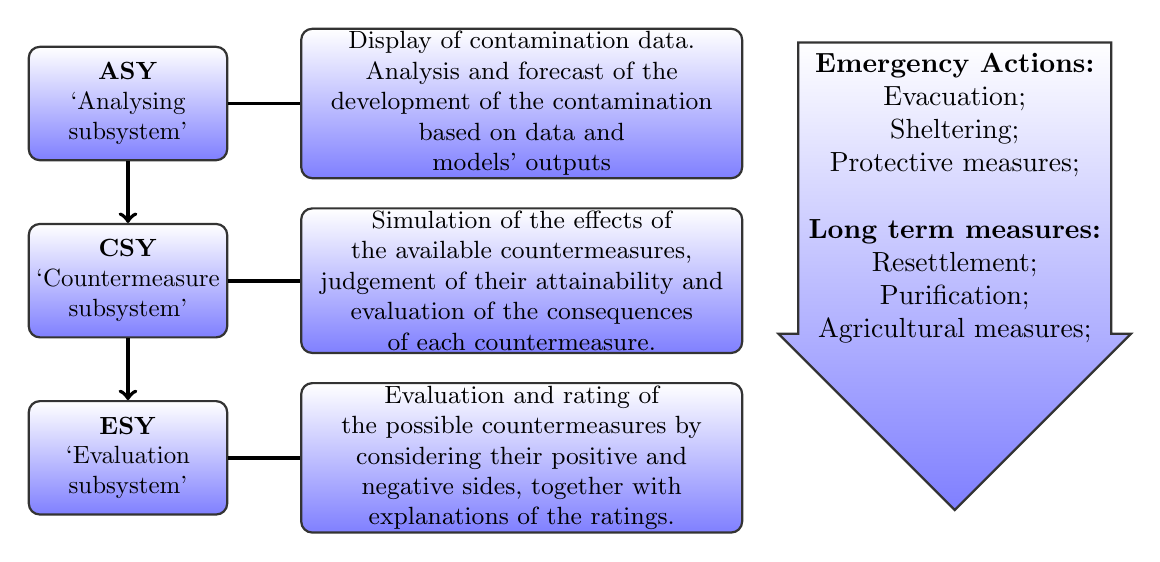
\begin{tikzpicture}
[ man/.style={rectangle, rounded corners,draw=black!80,top color=white, bottom color=blue!50, align=center, node distance=2.5cm, inner sep=0pt, minimum height=1.6cm, minimum width=2.8cm,  thick,scale=0.9},
 man1/.style={rectangle, rounded corners,draw=black!80,top color=white, bottom color=blue!50, align=center, node distance=5cm, inner sep=1pt, minimum height=1.6cm, minimum width=5.6cm, font=\small, thick, },]
\node[man] (A) {\textbf{ASY}\\ `Analysing\\ subsystem'};
\node[man] (B) [below of=A] {\textbf{CSY}\\ `Countermeasure\\ subsystem'};
\node[man] (C) [below of=B] {\textbf{ESY}\\ `Evaluation\\ subsystem'};
\node[man1](D)[right of=A]{Display of contamination data.\\ Analysis and forecast of the \\ development of the contamination\\ based on data and \\ models' outputs};
\node[man1](E)[right of=B]{Simulation of the effects of\\ the available countermeasures,\\ judgement  of their attainability and \\ evaluation of the consequences \\ of each countermeasure.};
\node[man1](F)[right of=C]{Evaluation and rating of \\ the possible countermeasures by \\ considering their positive and  \\ negative sides, together with\\ explanations of the ratings.};
\node[single arrow, shape border rotate =270, draw=black!80,align=center, node distance=4cm,top color=white, bottom color=blue!50, thick] (G) at (10.5,-1.2) {\textbf{Emergency Actions:} \\ Evacuation;\\ Sheltering;\\ Protective measures;\\  \\ \textbf{Long term measures:}  \\ Resettlement; \\ Purification; \\ Agricultural measures; };
\draw [->,line width=0.5mm](A) -- (B);
\draw [->, line width=0.5mm](B) -- (C);
\draw[-, line width=0.5mm] (A)--(D);
\draw[-, line width=0.5mm] (B)--(E);
\draw[-, line width=0.5mm] (C)--(F);
\end{tikzpicture}
\caption{Conceptual structure of RODOS from \citet{Leonelli2013} and after \cite{raskob2009}. The left column lists the subsystems, the central one describes the functionalities of each of these and the right one summarizes potential countermeasure both in the short and in the long term.}
\label{fig:fromBri}
\end{center}
\end{figure*} 

MCDA techniques were included into both the CSY and the ESY components to evaluate and rank potential countermeasures. It is important to note here the relevance of the explanation module within the ESY (as expressed in the bottom-central box of Figure \ref{fig:fromBri}). Empirical research has shown that DMs do not accept the suggestions of a system which does not provide a rationale for the outputs it produces, even if the system delivers accurate results  \citep{Papamichail2013}. Furthermore, as extensively discussed in \citet{French2009}, the ultimate objective of any decision analysis is not in simply choosing a decision which is considered to be optimal according to certain criteria, but more importantly in developing a deeper understanding of the values and the uncertainties of the problem studied. These insights may then lead to an evolution of the DMs' judgements and possibly to a revision of the whole model. This process is often called requisite modelling \citep{Phillips1984}. This idea was effectively included in the initial aims of both the development of RODOS and the International Chernobyl Project. Therefore RODOS includes a variety of features to justify its outputs, as for example a natural language report generator to explain the ranking of the policies \citep{Papamichail2003}, sensitivity analysis graphs and their interpretations \citep{Papamichail2005}.

The ASY subsystem is made of many different \textit{modules} (or component DSSs), each providing estimates and forecasts for a different aspect of the emergency as stated in the top central box of Figure \ref{fig:fromBri}. For instance, one of these modules concerns the workings of the source term estimating the likelihood of a release of contamination from the plant. Another one includes atmospheric diffusion models describing the spread of the contamination. Additional modules model the effect of this spread might have because of the exposure of  humans, animals and plants. Although the ASY modules are capable of working independently, in a comprehensive emergency management these are networked together in the sense that the outputs of some modules are used as inputs for others. Another important element to highlight from the above description is that the domains the ASY modules aim at describing are particularly heterogeneous and therefore require knowledge about a variety of different disciplines. In Figure \ref{networkino}, from \citet{Leonelli2013},  a plausible network of modules for use of a nuclear DSS is presented. Each vertex of the network corresponds to a module and two modules are connected by an arc if the outputs of the parent node are used as inputs for the child node (see Appendix \ref{appendixB} for an introduction to graph theory). The modules corresponding to the vertices of the network in Figure \ref{networkino} cover the main aspects of a nuclear emergency, as for example the overall workings of a nuclear power plant (Power plant and source term nodes), the spread of contamination (Air and Water dispersal and contamination) and the consequences the accident (Human health, Costs and Political effects). The nodes are grouped in such a way that vertices with the same color represent modules concerning the same domain of expertise. Specifically, the grey vertices are concerned with engineering issues; the green ones with the environment; the blue ones with biological consequences; the brown, red and yellow ones with the political, medical and economical outcomes, respectively. Furthermore, the edge set of the network in Figure \ref{networkino} describes plausible input/output relationships between the modules. So, for instance, the Deposition module uses as input only the outputs of the Water and Air dispersal modules, whilst Human absorption depends on Water dispersal, Animal absorption and Deposition since these are the main factors through which human can get in touch with the contamination. 
\begin{figure*}
\begin{center}
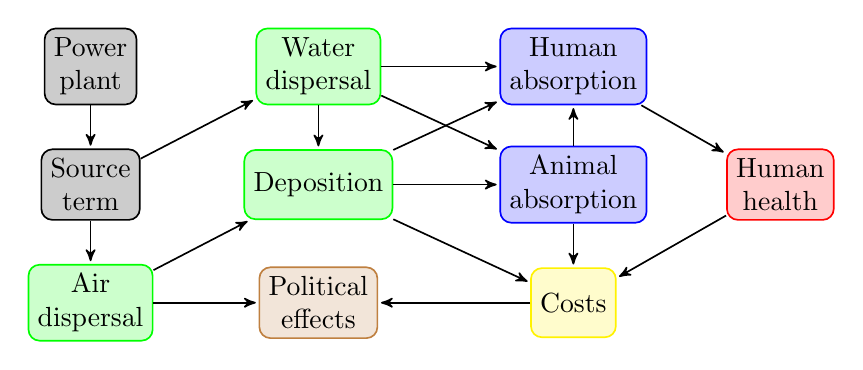
\begin{tikzpicture}[->,>=stealth',shorten >=1pt,auto,node distance=1.5cm,
                    semithick]
 \tikzstyle{every state}=[fill=white,draw,text=black, shape=rectangle, rounded corners,every text node part/.style={align=center}]
  \node[state]  (A)      [fill=black!20, draw=black!100, text=black]              {Power \\ plant};
  \node[state]         (B) [right = of A, draw=green!100, fill=green!20] {Water \\ dispersal};
   \node[state] (C) [draw=blue!100,  fill=blue!20,  right = of B]{Human \\ absorption};
\node[state] (D) [below of=A, fill=black!20, draw=black!100, text=black ]{Source \\  term};
\node[state](E)[below of=D, draw=green!100, fill=green!20]{Air \\ dispersal};
\node[state](F)[below of=B, draw=green!100, fill=green!20]{Deposition};
\node[state](H)[below of=F, draw=brown!100, fill=brown!20]{Political \\ effects};
\node[state] (L)[draw=blue!100,  fill=blue!20, text=black, below of =  C]{Animal \\ absorption};
\node[state](I)[below of=L, fill=yellow!20, draw=yellow!100]{Costs};
\node[state](G)[draw=red!100, fill=red!20, right=1cm of L]{Human \\  health};
\path (A) edge (D)
        (D) edge (B)
             edge (E)
         (B) edge (C)
              edge (L)
             edge (F)
          (E) edge (H)
               edge (F)
           (L) edge (C)
         (C) edge (G)
         (F) edge (L)
             edge (I)
             edge (C)
          (L) edge (I)
         (G) edge (I)
          (I) edge (H);
\end{tikzpicture}
\end{center}
\caption{Plausible network for the modules of a nuclear decision support system. \label{networkino}}
\end{figure*} 

Each of the modules of the ASY comprises a set of methodologies, either deterministic or stochastic, to perform the task they were designed for. As an example, \citet{Turner1994} lists dozens of different atmospheric dispersion models that have been applied to different domains and systems. From the very early stages of the development of RODOS it was recognised \citep[after considerable debate, as noted in][]{Smith1997} that stochastic, and more specifically, Bayesian inferential methodologies should be used in such a nuclear DSS to assimilate, combine and represent uncertainties. \citet{Smith1997} and our discussion in Section \ref{sec:early} extensively argued why it is reasonable to use this representation of uncertainty. Therefore, different Bayesian models have been developed for the different modules, as for example a BN for the workings of the source term \citep{Caminada2000}, a dynamic random forest for the atmospheric dispersion \citep{Smith1997} and a dynamic spatial model for the deposition module \citep{De2011}.  

It is also important to note here that in theory it could be possible for the ASY to consist of a single big module which models the whole domain of nuclear emergency management. However, the provision of the system to be used across all the European countries required the software to support the integration of external programs developed by national research institutes of the many involved countries. Therefore, the ASY had to be structured in this modular form, as a network of sub-models concerning the different elements of the emergency.

The description of the RODOS system for nuclear emergency management has highlighted the complexity of the domains that current  DSSs aim at describing. The main points to inherit from this section are the following:
\begin{itemize}
\item inference and forecasting need to be distributed among the different modules within the DSS;
\item the judgements and beliefs of different individual with different expertise need to be included in the inferential process;
\item computations need to be fast to allow for real-time decision making in case of an emergency;
\item MCDA techniques need to be included to reveal the true values of the DMs.
\end{itemize}

It is important to underline the scientific relevance of a project like the development of RODOS. Fortunately, although the consequences of a nuclear accident are and are perceived as severe and far-reaching,  the probability of occurrence of these is extremely low and RODOS is likely not to be used for actual emergency management \citep{Geldermann2009}.\footnote{\citet{Walle2008} noted that such a system could be actually used for different types of nuclear threats, as for example dirty bombs, although this type of aid is not publicly stated in the mission of RODOS.} At the same time, this implies that data and knowledge about this type of emergencies is scarce. The process of the construction of RODOS has actually deepened the understanding of both the values of potential DMs and the possible evolutions of the emergency. As noted in \citet{Papamichail2013}, nuclear emergency management has been at the forefront of both  stakeholder engagement and the use of decision conferencing, demonstrating the benefits of these techniques. Nowadays RODOS is not only used as an incommensurable educational tool for training personnel through exercises of scenario analysis, but also to highlight the areas in which current emergency management plans may not be adequate. \citet{Gering2013} reported a study where RODOS was used to simulate emergencies with features similar to the recent outworkings of the Fukushima nuclear plant and showed that current methodologies have several major problems. 

\section{Current Probabilistic Expert Systems}
\label{sec:current}
The complexity of the models that are currently built to tackle real applications, as the nuclear one, is increasing radically. The decomposition into local distributions that standard graphical models offer is not sufficient any more to both clearly depict the situation under study and allow for fast computations. Within the statistical graphical community, this was first recognised in \citet{Mahoney1996} for modelling military problems. The authors highlighted the need of an additional intermediate level of decomposition which breaks down the problem into a set of coupled components, both semantically and formally separable. Semantic separability implies that the component is meaningful to the user of the model, whilst formal separability means that the different components can be re-aggregated into a consistent probability model. This intermediate decomposition exactly corresponds to the division of the ASY component into networked modules within the RODOS system as in Figure \ref{networkino} and is indeed called in \citet{Mahoney1996} \textit{modularisation}.

\citet{Mahoney1996} referred to two attempts in the literature to create this intermediate level of modelling, namely similarity networks \citep{Heckerman1990} and  multi-sectioned BNs \citep{Xiang2002,Xiang2011}.  However, since both these attempts do not allow for enough modelling flexibility, they pointed towards the use of object oriented techniques in probabilistic modelling, similar to the ones used in programming languages. The authors noticed, as further stressed in \citet{Johnson2012}, that the object oriented paradigm provides features to simplify the modelling task in complex situations.  Specifically:
\begin{itemize}
\item \textbf{abstraction}/\textbf{encapsulation}: this means that some information is hidden to the user and its access is allowed only via a predefined interface. Modifications within these interfaces do not affect other parts of the system;
\item \textbf{modularisation}/\textbf{reuse}: the system is composed of a set of loosely connected units, which, if the interfaces are held fixed, can be changed without having to rebuild the whole model.
\end{itemize} 
These features are embedded in the IDSS methodology we introduce in this thesis and, by recalling the description of the nuclear DSS RODOS, are required if we are to develop support systems to be used in practice. 

The object oriented route for probabilistic graphical models then started with the development of Object Oriented Bayesian Networks (OOBNs) \citep{Koller97} and, concerning the modelling of complex situations, then continued in two main streams of research. The first one aimed at integrating first-order logic with Bayesian probability theory and culminated with the definition of multi-entity BNs \citep{Laskey2008, Laskey2009}. These can be represented as a collection MFrags \citep{Laskey1997}, which can be thought of as OOBNs with root nodes having known values. The other strand of research discusses the use of OOBNs as an integrating tool and introduced the concept of integrating BNs \citep{Johnson2012a}. An integrating BN can be thought of as a large OOBN where different probabilities are elicited by different groups of experts. These are a special case of IDSSs, but still represent an important step forward to the representation and elicitation of complex probabilistic models. These have been successfully applied to a variety of domains \citep{Johnson2013, Johnson2014,Mortera2013}.   

A completely different route from the object oriented paradigm in ESs has been proposed in \citet{Goldstein96}, which suggested the use of Bayes linear methodologies not requiring the specification of a full prior distribution \citep[see e.g.][]{Goldstein2007}. This approach simplifies both the computation and the elicitation burden, but does not provide in itself a viable alternative for the modelling of complex situations as the nuclear emergency management case described above.

Although all the above models can be used to support management decisions as noted in \citet{Johnson2014}, these do not include any formal representation of both the available decision space and the preferences of the DM, as required in the nuclear emergency management example. Influence Diagrams (IDs) are a class of graphical models  representing random variables, utilities and decisions \citep[see e.g.][and Section \ref{sec:id}]{Bielza2011,Howard2005,Jensen2013}. Of critical important is to  note that the literature about IDs does not provide many insights on the use of these models for the representation and modelling of complex situations. The main focus of ID's research has been on the improvement of the speed computations, either exact or approximated. Thus, although IDs include both decision and utilities, these  do not possess the expressive power of, for example, integrating BNs for the representation of current applied problems.

Before concluding this section, we note that the description of the nuclear emergency management domain highlighted the geographic nature of many problems that DMs have to deal with in practice. On one hand, this simply means that the dimensionality of the overall problem grows since each variable of the large system might be recorded and observed at different locations in space. On the other, it also raises issues specific of geographic modelling and concerning the use of geographic information systems in probabilistic models \citep{Stassopoulou1998}. Although we do not deal specifically with these issues, we recognise their importance in many applications and we note that there are now methods customised for the integration of geographic information systems with graphical models \citep{Laskey2010, Johnson2012}. However, in Section \ref{sec:exalgo} we present two examples of how a geographic component can be included into an IDSS in the simplest possible case.

\section{Decision Support Systems for the XXI Century}
\label{sec:decision}
Although the technology  reviewed in the previous section represents a big step forward in the modelling of complex issues, we note here that these methodologies still do not address many of the features of classes of problems as the nuclear emergency management of Section \ref{sec:nuclear}. 

First, because of the underlying OOBN assumption, most of the methods above assume that each submodel is a graphical one. This is a restrictive assumption and, as we saw, many statistical models, not necessarily graphical, have been already developed for some of the ASY components of RODOS. Furthermore some of the modules in use often are not probabilistic: this is the case for example of big simulators that model climate change. The technology of \textit{emulators} \citep[][and Section \ref{sec:emu}]{Kennedy2001, OHagan2006} can then be used  to introduce a probabilistic distribution over the outputs of such simulators. 

Second, RODOS implemented MCDA techniques to perform a formal decision analysis. Many current statistical ESs do not allow for such outputs and in general provide only probabilistic beliefs on a set of goal variables. Therefore, there is a need for new methods to be implemented in DSSs that have the power of performing MCDAs. In RODOS this was based on value functions. We argue here though that for current DSSs this is not sufficient and that multiattribute utility theory, enabling a full uncertainty handling, needs to be used as a representation of the DMs' preferences.      

Third, in such domains decision making is not usually the responsibility of a single individual but rather of groups. Decision centres will have the accountability and the responsibility of choosing a course of action and their judgements will be supported by best experts' knowledge. Therefore, DSSs need  to provide both a theoretical framework allowing for such a collaborative purpose and the technology  to support prescriptive team decision making.   

Lastly, in order for this to be feasible in practice, both probabilistic inferences and preferential modelling need to be distributed, as in the ASY, ESY, CSY structure of a system like RODOS. Therefore, the distributed nature of, for example, an integrating BN needs to embellished with a formal preferential analysis, which entertains the same distributed nature, both formally and semantically. 

It is therefore fundamental to develop a framework with the above features in order to properly support DMs in real current applications. As remarked by \citet{Mahoney1996}, the distributed nature of such a methodology is vital, since the following benefits would follow:
\begin{itemize}
\item computational tractability;
\item comprehensibility;
\item feasibility of testing.
\end{itemize}
Computational tractability derives from the local computation structure associated to distributed systems \citep[widely studied in machine learning, see e.g.][]{Peteiro2013,Rodriguez2011}. Distributed systems are more comprehensible since the overall outputs can be traced back to each subsytem's outputs, providing much clearer justifications of the delivered estimates. Finally, feasibility of testing follows since each subsystem can be more straightforwardly tested and potentially upgraded than the whole system at once.  In the following we highlight how the IDSS methodology we introduce here entertains such features.

As with the motivations that lead to the inception of graphical modelling techniques, we can notice that distributivity in complex systems aims at breaking down   a huge problem into ones of smaller dimension. In \citet{Spiegelhalter1993} such a modelling approach was referred to as \textit{divide-and-conquer}. The methodology of IDSSs uses the same idea to simplify decision analyses in highly multivariate and heterogeneous problems. We note here that such an approach is commonly used in a variety of domains and subjects, as for example in composite likelihood methods \citep{Varin2011}, Markov chain Monte Carlo  schemes \citep{Lindsten2014} and parallel computing \citep{Chandy1998}.   

\section{Contributions of the Thesis}
\label{sec:contributions}
In this thesis we develop a methodology that addresses the gaps of current ESs we listed in Section \ref{sec:decision} to model complex domains. We call our methodology an \textbf{IDSS}, which embeds a formal distributed Bayesian decision analysis combining the beliefs of different of groups of experts. Throughout the thesis we specify the conditions enabling such an integration in a variety of frameworks and discuss the advantages of this methodology. We then provide a toolkit of methods for inference and decision making in an IDSS by, for instance, developing propagation algorithms and symbolic methodologies.

From a more specific/domain-based viewpoint, the results in this thesis extend current methods on a variety of aspects:
\begin{itemize}
\item in Chapter \ref{chapter3} we extend standard independence notions over the parameter vectors of a variety of graphical models \citep[see e.g.][]{Spiegelhalter1990,Dawid1993, Freeman2011} enabling distributed multi-expert inferences in IDSSs;
\item there are now several rules to combine expert judgement in the literature \citep[see e.g.][]{French2011}. Our work extends such rules for complex multivariate domains where the overall probability distribution can be described by means of a graphical model (see e.g. Propositions \ref{prop:combi} and \ref{prop:dyncombi});
\item a new concept of statistical causality tailored to the needs of an IDSS is defined in Section \ref{sec:idsscaus}. We are able to show that the standard definition of causality of \citet{Pearl2000} represents a special case of our definition;
\item we introduce a new class of utility factorisations in Section \ref{sec:comput} customised to the needs of an IDSS, allowing for a distributed computation of Bayesian expected utilities in the multi-expert domains we address;
\item we  introduce in Section \ref{sec:algorithms} new utility-based propagation algorithms for the distributed computation of expected utility scores in IDSSs. Some of the current evaluation algorithms of decisional structures can be seen as special cases of the ones we define here;
\item we deduce new recursions for the computations of moments of functions over the vertices of an agreed graphical model, generalising the ones of \citet{Cowell1999a} and \citet{Nilsson2001};
\item by studying decision making in an IDSS from an algebraic perspective, we identify minimal sets of independence statements assuring the system provides rational decision support. This recognition leads us to define in Section \ref{sec:momind} new types of independence tailored to the needs of an IDSS; 
\item we develop in Section \ref{sec:short} new symbolic approaches to decision making in different frameworks, which extends current symbolic methods for probabilistic reasoning in graphical models \citep[see e.g.][]{Castillo1997, Darwiche2003}.
\end{itemize}
More detailed explanations of how our results generalise current methodologies can be found in the following chapters. 

In this thesis we almost exclusively focus on the technical conditions that guarantee the existence of an IDSS. In order to concisely illustrate this methodology, our examples necessarily need to be small-dimensional. However, as we discuss more extensively in the following chapters, our methods would scale up to larger real-world examples because of the distributed nature of IDSSs.

The material of this thesis has appeared/will appear in seven papers I have co-authored with my supervisor Jim Smith and other collaborators. Additional details about these papers can be found in the Declaration on page \pageref{declaration}. 
\section{Structure of the Thesis}
\label{sec:structure}
Having extensively discussed the need for an IDSS and reviewed other statistical approaches to model complex domains in this first chapter, in Chapter \ref{chapter2} we survey classical Bayesian decision analysis methods. We then discuss  standard Bayesian reasoning and the Subjective Expected Utility (SEU) methodology for decision making. We introduce a variety of probabilistic, utility and decision models. We further survey issues associated to group decision making and the use of expert judgement. 

In Chapter \ref{chapter3} we introduce IDSSs and a set of axioms that can guarantee their existence. We then discuss what makes a \lq{g}ood' IDSS  and generic conditions that can ensure a good IDSS both a priori and after the introduction of both observational and experimental data.  We then show that many of the statistical models introduced in Chapter \ref{chapter2} can be used as an underlying probabilistic framework for an IDSS and discuss the conditions that these need to entertain. 

We then consider in Chapter \ref{chapter4} a large class of IDSSs based on flexible probability and utility models. For this class we develop distributed utility-based propagation algorithms that allow for the exact computation of expected utility scores from the outputs of the individual modules of the IDSS. We then exemplify the methodology at the end of the chapter in a variety of domains. 

The expressions used by the IDSS to rank the available policies are often polynomial functions of the outputs of the component DSSs. This recognition lead us to analyse IDSSs in Chapter \ref{chapter5} from an algebraic viewpoint and to define independence concepts following from the polynomial relationships existing between these outputs. We then introduce symbolic techniques for particular statistical models in IDSSs, which are intimately linked with algebraic analyses. 

We conclude the thesis in Chapter \ref{chapter6}, where we summarise the main results of the thesis and discuss possible extensions of the methods developed in the thesis. 

The thesis also include 5 appendices. In Appendix \ref{appendixA} we collect longer proofs. Appendix \ref{appendixB} introduces the required terminology of graph theory. Appendix \ref{appendixE} reviews basic statistical distributional theory and standard Bayesian models. Appendix \ref{appendixC} consists of basic definitions of polynomial algebra. In Appendix \ref{appendixD} we report our computer algebra code to implement the methods we introduce in Section \ref{sec:symbolic}. 
\chapter{Classical Bayesian Decision Analysis} % Main chapter title

\label{chapter2} % For referencing the chapter elsewhere, use \ref{Chapter1} 

\lhead{Chapter 2. \emph{Classic Bayesian Decision Analysis}}

In the introduction we discussed the use of Bayesian reasoning and modelling techniques at the inception of probabilistic ESs. Although we noted the inappropriateness of standard methodologies for the needs of current applications, several systems are still based on these traditional models. The theory we develop in the following chapters is a generalisation of Bayesian methodologies and models to formally accommodate the beliefs of different group of experts. We need therefore first to provide a broad overview of the currently available Bayesian modelling tools for DMs. 

The chapter is structured as follows. In Section \ref{sec:bayesianreasoning} we outline the Bayesian formalism of inference. Section \ref{sec:SEU} introduces the Subjective Expected Utility (SEU) methodology which embeds canons of rational decision making and defines rules to make decisions that are optimal according to these canons. The SEU model basically consists of two main ingredients: a probability function, representing the beliefs of a DM, and a utility function, representing her values. Sections \ref{sec:prob} and  \ref{sec:ut} introduce methodologies to represent respectively probability and utility functions in a multivariate setting. In such a case the definition and elicitation of these functions is often prohibitive. Independence concepts have been introduced to factorise these into subfunctions with a smaller number of arguments. Such factorisations can  often be depicted by a graph providing a powerful and intuitive representation of the relationships between the elements of the problem. Therefore our discussion is mainly based on graphical models, for both probabilities and utilities. We introduce here a new subclass of certain utility graphical models defined in \citet{Abbas2010} that have interesting properties in the domains we address in this thesis \citep[see also][]{Leonelli2015}.

In Section \ref{sec:dec} we introduce classes of models that explicitly represent both probabilities and utilities, and the decisions available to a single DM. Again our discussion focuses on graphical models and in particular on the Influence Diagram (ID) model. We consider in this thesis the models class of multiplicative IDs defined in \citet{Leonelli2015a} and introduce a new fast evaluation algorithm for these models.

The SEU model is only capable of representing how a single DM should rationally commit to decisions. However, as we have seen in Chapter \ref{chapter1}, policy choices are seldom made by just one person. There might be several DMs sharing the authority and responsibility of choosing a certain policy, many stakeholders who are affected by the DM's decision, and experts that are consulted by the DMs. In Section \ref{sec:group} we briefly review the literature on both group decision making and the use of expert judgement to support decision making. We then conclude with a more detailed explanation of the contributions of this thesis and a discussion.

\section{Bayesian Reasoning}
\label{sec:bayesianreasoning}
\subsection{The Full Probabilistic Case}
A problem domain is denoted by an often large dimensional random vector $\bm{Y}$ with sample space $\bm{\mathcal{Y}}$. We denote by $\bm{y}$ a generic instantiation of $\bm{Y}$ and we let $\bm{\theta}\in\bm{\Theta}$ parametrise the density function $f$ of $\bm{Y}$. In a Bayesian framework the parameter $\bm{\theta}$ is itself a random variable. We let $\pi$ denote its density function. For the purpose of this section, the vectors are assumed to be continuous.\footnote{In discrete domains integrals are simply substituted by summations. We denote probability mass functions by $p$.}  Let $\bm{X}$ be a random vector sampled from the same population as $\bm{Y}$ providing some data points $\bm{x}$. Within this framework, \textbf{Bayes theorem} can be  simply  employed to update the beliefs about $\bm{\theta}$ after evidence $\bm{x}$ has been observed as 
\begin{equation}
\label{eq:bayes}
\pi(\bm{\theta}\;|\;\bm{x})=\frac{f(\bm{x}\;|\;\bm{\theta})\pi(\bm{\theta})}{f(\bm{x})}=\frac{f(\bm{x}\;|\;\bm{\theta})\pi(\bm{\theta})}{\int_{\bm{\Theta}}f(\bm{x}\;|\;\bm{\theta})\pi(\bm{\theta})\dr \bm{\theta}}.
\end{equation}
The terms of equation (\ref{eq:bayes}) have all a meaning. The so called \textit{prior distribution}, $\pi(\bm{\theta})$, represents the beliefs of the DM about the parameter $\bm{\theta}$ before evidence $\bm{x}$ is introduced into the system. If for example $\bm{Y}$ were a univariate binary random variable, then $\pi(\bm{\theta})$ would simply be a probability distribution over $[0,1]$ representing the beliefs of the DM about the probability of a success (for simplicity here we have chosen a discrete example). Although we do not further discuss these issues, we note that there is now an extensive literature and several software that allow for a faithful elicitation of such prior beliefs \citep[see e.g.][]{O'Hagan2006a}. The other term at the numerator, $f(\bm{x}\;|\;\bm{\theta})$, is usually called a \textit{likelihood function}. In a Bayesian setting this measures the DM's degree of belief in the data taking certain values given that the parameter is fixed to a certain hypothetical value. Continuing the example above, the likelihood would be in this situation the density of a Bernoulli random variable with a hypothetical unknown probability of success. The denominator of equation (\ref{eq:bayes}), $f(\bm{x})$,  simply corresponds to a normalising constant, since for a Bayesian all the relevant information is related to $\bm{\theta}$. Therefore, equation (\ref{eq:bayes}) is often presented in the following form,
\begin{equation}
\label{eq:proprbayes}
\pi(\bm{\theta}\;|\;\bm{x})\propto f(\bm{x}\;|\;\bm{\theta})\pi(\bm{\theta}),
\end{equation}
where $\propto$ corresponds to proportionality.  The corresponding normalising constant is often difficult to compute, since it requires an integration over an arbitrarily large space. Thus, equation (\ref{eq:proprbayes}) often represents a computationally less intensive version of equation (\ref{eq:bayes}). Finally, the \textit{posterior} distribution, $\pi(\bm{\theta}\;|\;\bm{x})$, is simply the revised density function of $\bm{\theta}$ after  evidence $\bm{x}$ has been observed. Suppose, for instance, that $\bm{x}$ in the running example is the result of ten coin tosses showing all head (or 1) and assume that the prior distribution was symmetric around 1/2. The posterior distribution would then be left-skewed and values in the interval $(1/2,1]$ would have in general higher probability than the ones in $[0,1/2]$. Henceforth, we assume all these densities to represent the subjective Bayesian beliefs of a DM \citep[for more details on the various interpretation of probabilities and the adequateness of the Bayesian interpretation in decision making, see e.g.][]{O'Hagan2004a,French2000b}.

Depending on whether the variables are continuous or discrete, on their support and  on the domain under study, there exist many different possible choices for both the likelihood function and the prior density. We review a variety of standard models in Appendix \ref{appendixE}, as for example the Bayesian Normal linear model, which assumes a Normal distribution for both the likelihood and the prior density of the mean when the variance is assumed to be known. We note here that a computationally efficient choice of prior and likelihood are of two that are \textit{conjugate} \citep{Bernardo2009, O'Hagan2004a}. This is the case whenever the posterior, computed via Bayes theorem, lies in the same family of distributions as the prior. In the example above, if $\pi(\bm{\theta})$ were chosen to follow a Beta distribution with parameters $(a,b)\in\mathbb{R}^2_{>0}$, then the posterior would also be a Beta with some new parameters $(a',b')\in\mathbb{R}^2_{>0}$ (see Appendix \ref{sec:beta}).

Implicitly in equation (\ref{eq:bayes}) we assumed that the parameters of the distribution of $\bm{\theta}$ were known. Within the Bayesian approach this does not necessarily have to be  the case and several different levels or layers of uncertainty can be introduced. This modelling strategy is usually referred to as multilevel or \textit{hierarchical modelling} \citep{Gelman2006}. For example, the parameters of the Beta distribution above, $a$ and $b$, could have been assumed to be random and depending on some other parameters, which could have further been random variables, and so forth. For the purpose of this thesis, we only consider hierarchies consisting of one layer so that the parameters of $\pi(\bm{\theta})$ are known. These are usually referred to as \textit{hyperparameters}. 

\subsection{Moments}
Density functions can be easily summarised using the notion of \textit{moments}, which can describe some of their features. Moments are expected values of power functions of random variables. To introduce these, we first define the concept of expected  values. Let $g:\bm{\mathcal{Y}}\rightarrow \bm{\mathcal{Y}}'$, i.e. $g$ is a function mapping elements of $\bm{\mathcal{Y}}$ into $\bm{\mathcal{Y}}'$. 

\begin{definition}
\label{def:expectedvalue}
The expected value of $g(\bm{Y})$ is defined as\footnote{In the discrete case equations (\ref{eq:exp}) and (\ref{eq:condexp}) have a slightly different form which is not relevant for this thesis and can be found in \citet{Casella2002}.}
\begin{equation}
\label{eq:exp}
\E(g(\bm{Y}))=\int_{\bm{\mathcal{Y}}'}g(\bm{y})f(\bm{y})\dr \bm{y}=\int_{\bm{\Theta}}\E(g(\bm{Y})\;|\;\bm{\theta})\pi(\bm{\theta})\dr \bm{\theta},
\end{equation}
where the expected value $\E(g(\bm{Y})\;|\;\bm{\theta})$ conditional  on $\bm{\theta}$ is defined as
\begin{equation}
\label{eq:condexp}
\E(g(\bm{Y})\;|\;\bm{\theta})=\int_{\bm{\mathcal{Y}}'}g(\bm{y})f(\bm{y}\;|\;\bm{\theta})\dr\bm{y}.
\end{equation}
\end{definition}
For continuity with the previous section, we considered in Definition \ref{def:expectedvalue} quantities conditional on the parameter vector $\bm{\theta}$. However, in general, the conditioning might operate over any random vector of interest.

We can now define the notion of moment. Let, for $n\in\mathbb{Z}_{\geq 1}$, $[n]=\{1,\dots,n\}$, $\bm{s}^\T=(s_1,\dots,s_n)=(s_i)_{i\in[n]}\in \mathbb{Z}_{\geq 0}^n$ and $\bm{Y}^{\bm{s}}=Y_1^{s_1}\cdots Y_n^{s_n}$. 

\begin{definition}
We say that the moment of \emph{order} $\bm{s}$ of $\bm{Y}$ is $\E\left(\bm{Y}^{\bm{s}}\right)$. The moment of order $\bm{s}$ of $\bm{Y}$ conditional on $\bm{\theta}$ is $\E\left(\bm{Y}^{\bm{s}}\;|\;\bm{\theta}\right)$. 
\end{definition}

 We now define some specific moments.

\begin{definition}
Let $\bm{Y}$, $\bm{Y}_i$ and $\bm{Y}_j$ be  random vectors of dimension $n$. The \emph{expectation} of $\bm{Y}$ is $\E(\bm{Y})=\E(\bm{Y}^{\bm{1}})$,  where $\bm{1}$ is a vector of dimension $n$ with $1$ in each entry, whilst the \emph{variance} of $\bm{Y}$, $\V(\bm{Y})$, is $\E((\bm{Y}-\E(\bm{Y}))(\bm{Y}-\E(\bm{Y}))^\T)$. The \emph{covariance} between $\bm{Y}_i$ and $\bm{Y}_j$, $\Cov(\bm{Y}_i,\bm{Y}_j)$, is $\E((\bm{Y}_i-\E(\bm{Y}_i))(\bm{Y}_j-\E(\bm{Y}_j))^\T)$. 
\end{definition}

\begin{definition}
Let $\bm{Y}$, $\bm{Y}_i$ and $\bm{Y}_j$ be  random vectors of dimension $n$. The \emph{conditional expectation} of $\bm{Y}$ given $\bm{\theta}$ is $\E(\bm{Y}\;|\;\bm{\theta})=\E(\bm{Y}^{\bm{1}}\;|\;\bm{\theta})$, whilst the \emph{conditional variance} of $\bm{Y}$ given $\bm{\theta}$, $\V\left(\bm{Y}\;|\;\bm{\theta}\right)$, is $\E\left(\left(\bm{Y}-\E(\bm{Y}\;|\;\bm{\theta})\right)(\bm{Y}-\E(\bm{Y}\;|\;\bm{\theta})\right)^\T\;|\;\bm{\theta})$. The \emph{ conditional covariance} between $\bm{Y}_i$ and $\bm{Y}_j$ given $\bm{\theta}$, $\Cov(\bm{Y}_i,\bm{Y}_j\;|\;\bm{\theta})$, is $\E((\bm{Y}_i-\E(\bm{Y}_i\;|\;\bm{\theta}))(\bm{Y}_j-\E(\bm{Y}_j\;|\;\bm{\theta}))^\T\;|\;\bm{\theta})$.
\end{definition}
We now list some properties of these operators \citep[see e.g.][]{Casella2002}.
\begin{proposition}
\label{prop:propmom}
Let $\bm{Y}_i$ and $\bm{Y}_j$ be random vectors of dimension $n$. Further let $B_i$ and $B_j$ be $n\times n$ matrices with real entries, whilst $\bm{b}\in\mathbb{R}^n$. The following identities hold. 
\begin{align}
\E(B_i\bm{Y}_i\pm B_j\bm{Y}_j\pm \bm{b}\;|\;\bm{\theta})&=B_i\E(\bm{Y}_i\;|\;\bm{\theta})\pm B_j\E(\bm{Y}_j\;|\;\bm{\theta}) \pm \bm{b},\nonumber\\
\Cov(\bm{Y}_i,\bm{Y}_j\;|\;\bm{\theta})&=\E\left(\bm{Y}_i\bm{Y}_j^\T\;|\;\bm{\theta}\right)-\E(\bm{Y}_i\;|\;\bm{\theta})\E(\bm{Y}_j\;|\;\bm{\theta})^\T,\nonumber\\
\V(B_i\bm{Y}_i \pm B_j\bm{Y}_j\pm \bm{b}\;|\;\bm{\theta})&=B_i\V(\bm{Y}_i\;|\;\bm{\theta})B_i^\T+B_j\V(\bm{Y}_j\;|\;\bm{\theta})B_j^\T\pm 2B_i\Cov(\bm{Y}_i,\bm{Y}_j\;|\;\bm{\theta})B_j.\nonumber
\end{align}
\end{proposition}

The following proposition then links conditional and unconditional moments of order one and two.

\begin{proposition}
\label{prop:towerrules}
Let $\bm{Y}_i$ and $\bm{Y}_j$ be two random vectors. Then
\begin{align}
\E(\bm{Y}_i)&=\E(\E(\bm{Y}_i\;|\;\bm{\theta})),\label{eq:tower}\\
\V(\bm{Y}_i)&=\E(\V(\bm{Y}_i\;|\;\bm{\theta}))+\V(\E(\bm{Y}_i\;|\;\bm{\theta})).\label{eq:totalvariance}
\end{align}
\end{proposition}
Equations (\ref{eq:tower}) and (\ref{eq:totalvariance}) are usually called \textit{tower rules} of moments. Specifically, equation (\ref{eq:tower}) is the tower rule of expectations, whilst equations (\ref{eq:totalvariance}) is referred to as \textit{law of total variance}.
 \citet{Brillinger1969} generalised the identities (\ref{eq:tower})-(\ref{eq:totalvariance}) and deduced a recursive formula to compute cumulants of any finite order. Cumulants can be thought of as a function of the moments, and vice versa. Many properties of random vectors can be more easily investigated using cumulants than moments \citep[see e.g.][]{Zwiernik2012}.

\section{The Subjective Expected Utility Model}
\label{sec:SEU}
In the previous section we introduced the Bayesian framework for reasoning about and modelling uncertainty. However, the Bayesian approach further provides an axiomatic basis for decision making, which embodies canons of rationality, usually referred to as the \textbf{SEU} model. Broadly speaking this consists of three main components:
\begin{itemize}
\item a decision space $\bm{\De}$ which includes the decisions $\bm{d}\in\bm{\De}$ available to the DM;
\item a probability density $f$ over the unknown state $\y\in \bm{\MY}$ of a vector of relevant random variables $\Y$;
\item a utility function $u(\bm{d},\bm{r}(\y,\bm{d}))$ describing the DM's preferences over some random vector $\bm{R}$, whose instantiation $\bm{r}=\bm{r}(\y,\bm{d})$ is a function of both $\bm{d}$ and $\y$, and takes values in $\bm{\Rs}$.
\end{itemize}

Having dealt with probability in Section \ref{sec:bayesianreasoning}, we now focus on utility functions.
\begin{definition}
\label{def:ut}
A utility function with arguments $\bm{d}$ and $\bm{r}$ is a real-valued function unique up to increasing affine transformations, $u:\bm{\De}\bigtimes\bm{\Rs}\rightarrow \mathbb{R}$, such that 
\begin{equation*}
\label{eq:utility}
\forall \; (\bm{d}_i,\bm{r}_i), (\bm{d}_j,\bm{r}_j)\in \bm{\De}\bigtimes\bm{\Rs},\;\; u(\bm{d}_i,\bm{r}_i)\geq u(\bm{d}_j,\bm{r}_j) \Leftrightarrow (\bm{d}_i,\bm{r}_i) \succeq (\bm{d}_j,\bm{r}_j),
\end{equation*}
where  $(\bm{d}_i,\bm{r}_i) \succeq (\bm{d}_j,\bm{r}_j)$ means that the DM finds that $(\bm{d}_i,\bm{r}_i)$ is at least as preferable as $(\bm{d}_j,\bm{r}_j)$. The $\bigtimes$ denotes the Cartesian product.
\end{definition}
Note that in general utility functions only represent preference rankings and do not include any representation of the strength of these preferences. Formally, utilities are only unique up to increasing affine transformations. Therefore, utility functions are usually normalised so that they take values between 0 and 1, i.e. $u:\bm{\De}\bigtimes\bm{\Rs}\rightarrow [0,1]$. There have been some theoretical studies considering strength of preferences \citep[see e.g.][]{Argyris2014}, but these are not considered in this thesis. 

The study of utility functions dates back to the work of \citet{VonNeumann2007} which mostly concerned the theory of games. Throughout the following years, several different authors derived different constructions of the SEU model based on different, but related, sets of axioms \citep[e.g.][]{Anscombe1963,DeGroot2005,Savage1972}.  We assume throughout the thesis that a set of axioms underpinning the SEU model holds and that the DM is able to elicit both a utility function and a probability distribution respecting one of these.

Now that utility functions have been introduced, we can show how the SEU model combines probabilities and utilities to guide decision making. Decisions are ranked according to their associated expected utility.

\begin{definition}
Let $\bm{\mathcal{D}}$ be a decision space, $f$ a density function for a random vector $\bm{Y}$ parametrised by $\bm{\theta}$ and $u$ a utility function with arguments $\bm{d}\in \bm{\mathcal{D}}$ and $\bm{r}=\bm{r}(\bm{y},\bm{d})$. The \textbf{expected utility} of a decision $\bm{d}$, $\bar{u}(\bm{d})$, is defined as
\begin{align}
\label{eq:expectedut}
\bar{u}(\bm{d})=&\int_{\bm{\Theta}}\bar{u}(\bm{d}\;|\;\bm{\theta})\pi(\bm{\theta}\;|\;\bm{d})\dr \bm{\theta},\\
\intertext{where}
\label{eq:expectedcondut}
\bar{u}(\bm{d}\;|\;\bm{\theta})=&\int_{\bm{\MY}}u(\bm{r},\bm{d})f(\y\;|\;\bm{\theta},\bm{d})\dr\y,
\end{align}
is the \textbf{conditional expected utility}.
\end{definition}
\begin{definition}
We say that a decision $\bm{d}^*\in\bm{\mathcal{D}}$ is \textbf{optimal} if $\bm{d}^{*}$ maximises the expected utility, i.e.
\begin{equation}
\label{eq:maxut}
\bm{d}^*=\arg\max_{\bm{d}\in\bm{\De}}\bar{u}(\bm{d}).
\end{equation}
\end{definition}

A few important points need to be made here. First, we underline that the SEU describes rational decision making of a single DM and there is no clear extension of this model to groups of DMs (see Section \ref{sec:group}). Second, the utility function, in contrast to value functions considered for example within RODOS, are able by construction  to model attitudes towards risk \citep[see e.g.][]{Keeney1993a}. Lastly, we remark that the SEU model falls within the class of normative approaches to decision making. From a set of axioms describing rationality, normative approaches are then able to produce a ranking of the available actions. However, there is a huge body of empirical literature which shows that people do not make decisions according to the SEU model \citep{Tversky1974}. This observation led on one hand to the development of extensions of the model \citep[e.g. prospect theory,][]{Kahneman1979}, and on the other to a different use of normative models to support DMs instead of automatically selecting optimal decisions. For example, the SEU model can be implemented into a DSS simply in order to allow the DM to explore the effects of her judgements on the ranking of the actions available to her.

Although equations (\ref{eq:expectedut}) and (\ref{eq:expectedcondut}) easily describes how expected utility can be computed, we note that in multivariate and dynamic settings the elicitation of both the utility function and the density function is often hard. Therefore, several concepts of independence and different modelling strategies have been discussed in the literature. We  first review the methods developed for the density $f$ and after for the utility function $u$. Another difficulty arises because of the maximisation in equation (\ref{eq:maxut}) when $\bm{\De}$ is high-dimensional. We  show in Section \ref{sec:dec} methods that decompose the maximisation process to take place into smaller spaces and therefore be computationally simpler. 
   
\section{Probability Models}
\label{sec:prob}
In this section we introduce a variety of models that decompose a probability density $f$ into smaller dimensional (conditional) densities. Our discussion focuses on graphical models since these can more easily describe the qualitative features underlying a domain of interest, a property that turns out to be fundamental for the developments of this thesis. We first introduce in Section \ref{sec:condind} the notion of conditional independence which is at the basis of the decomposition generated by graphical models. We then review non-dynamic and dynamic models in Sections \ref{sec:nondym} and \ref{sec:dynmod} respectively. In Section \ref{sec:causality} we introduce the notion of statistical causality and explain its importance within Bayesian reasoning. We conclude with a discussion in Section \ref{sec:emu} of the use probabilistic emulators. These  describe through a probability density the outputs of a complex deterministic function arising for example from complex computer codes. 
 
For ease of notation we leave the dependence on the decision $\bm{d}$ implicit in this section. However, although not explicitly labelled, the results below need to hold for every possible decision in $\bm{\mathcal{D}}$.
 
\subsection{Conditional Independence}
\label{sec:condind}
As discussed in Chapter \ref{chapter1}, graphical models can be underpinned by a conditional independence structure  \citep{Dawid1979} allowing for a formal modularisation of a model. Although conditional independence can be generally thought of as a tertiary operator - $\cdot \independent \cdot \;|\; \cdot$ - exhibiting a set of properties \citep[see e.g.][]{Dawid1993, Smith1989}, we formally define it for random variables and vectors only. It is important to point out that recently \citet{Dawid2014} generalised the notion of conditional independence to include both non-stochastic and stochastic variables and called it \textit{extended conditional independence}, which entertains the same properties of of standard conditional independence.

For the purpose of this section, let $A$, $B$ $C$ and $D$ be disjoint subsets of $[n]$, $\bm{Y}_A$, $\bm{Y}_B$, $\bm{Y}_C$ and $\bm{Y}_D$ be random vectors, and  $g$ denote a generic function.

\begin{definition}
We say that $\bm{Y}_A$ is independent $\bm{Y}_B$ given $\Y_C$, $\Y_A\independent \Y_B \;|\; \Y_C$, if 
$
f(\y_A,\y_B,\y_C)=f(\y_A\;|\;\y_C)f(\y_B,\y_C).
$
\end{definition}
 The conditional independence statement $\Y_A\independent \Y_B \;|\; \Y_C$ asserts that the only information to infer $\Y_A$ from $\Y_B$ and $\Y_C$ is from $\Y_C$.  \citet{Dawid1979} showed that the conditional independence operator has the following properties.
\begin{proposition}
\label{prop:semigraph}
It holds that:
\begin{enumerate}
\item $\Y_A\independent \Y_B \;|\;\Y_C \Longleftrightarrow \Y_B\independent \Y_A \;|\;\Y_C $;
\item $\Y_A\independent \Y_B \;|\;\Y_C \Longrightarrow g(\Y_A)\independent \Y_B \;|\;\Y_C$;
\item $\Y_A\independent \Y_B \;|\;\Y_C \Longrightarrow \Y_A\independent \Y_B \;|\;\Y_C, g(\Y_A)$;
\item $\Y_A\independent \Y_B \;|\;\Y_C$ and $\Y_A\independent\Y_D\;|\;\Y_B,\Y_C \Longleftrightarrow \Y_A\independent\Y_D,\Y_B\;|\;\Y_C$.
\end{enumerate}
\end{proposition}
We refer throughout the thesis to the condition in point 1 as the \textit{symmetry property}, whilst point 4 is usually referred to as \textit{strong decomposition}. These properties of conditional independence are usually called \textit{semi-graphoid axioms}.

Note that, although conditional independence is deeply linked to particular factorisations of densities, it is qualitative in nature and therefore easier to identify and justify.

\subsubsection{Context Specific Independence.}
The notion of conditional independence is only able to describe statements of the form $\Y_A\independent \Y_B \;|\;\Y_C $ holding for every instantiation $\bm{y}_C\in \bm{\MY}_C$, where $\bm{\MY}_C$ is the sample space of $\bm{Y}_C$. However, often this does not have to be the case and a domain can exhibit some independences only for subspaces of the sample space. \textit{Context specific} independences are able to depict this more general scenario \citep{Boutilier1996}. 

\begin{definition}
Let $\bm{\MY}_D'$ be a subspace of $\bm{\MY}_D$, the sample space of $\bm{Y}_D$. We say that $\Y_A$ and $\Y_B$ are contextually independent given $\Y_C$ and context $\y_D\in\bm{\MY}_D'$ if
\begin{equation*}
f(\y_A,\y_B,\y_C,\y_D)=f(\y_A\;|\;\y_C,\y_D)f(\y_B,\y_C,\y_D), \hspace{1cm} \mbox{ for } \y_D\in\bm{\MY}_D'.
\end{equation*}
\end{definition} 

In Sections \ref{sec:tree} and \ref{sec:CEG} we introduce two classes of models that can graphically  model this more general class of conditional independence statements. 
 
\subsection{Non Dynamic Models}
The notions of conditional independence introduced in Section \ref{sec:condind} is now exploited to define various types of models in a non-dynamic framework, i.e. when there is no recursive updating through time of the involved probabilities. Let $\Y=(Y_i)^\T_{i\in[n]}$ be a vector of random variables with sample space $\bm{\mathcal{Y}}=\bigtimes_{i\in[n]}\mathcal{Y}_i$, where $\mathcal{Y}_i$ is the sample space of $Y_i$, $\bm{y}\in\bm{\mathcal{Y}}$ and $y_i\in\mathcal{Y}_i$, $i\in[n]$. Let $\bm{\theta}_A$, taking values in $\bm{\Theta}_A$, parametrise the (conditional) density of $\bm{Y}_A$ having sample space $\bm{\mathcal{Y}}_A=\bigtimes_{i\in A}\mathcal{Y}_i$, $A\subseteq [n]$. Let $\bm{\theta}=(\bm{\theta}_i^\T)^\T_{i\in[n]}$  be the parameter associated to the density of $\bm{Y}$ taking values in $\bm{\Theta}$.

\label{sec:nondym}
\subsubsection{Independence Models.}
The simplest non dynamic model is the so called \textit{independence model}.
\begin{definition}
\label{def:indmodel}
An \emph{independence model} for $(\bm{Y},\bm{\theta})$ is such that $\independent_{i\in[n]} Y_i\;|\;\bm{\theta}$.
\end{definition} 
The independence model class can be simply described by a graph with vertex set  $\{Y_i:i\in[n]\}$ and empty edge set.
 
\subsubsection{Bayesian Networks.}
\label{sec:BN}
BNs \citep{Pearl1988a, Jensen2009, Korb2003, Lauritzen1996a, Smith2010} are the graphical model  most widely used  in practice. There are now thousands of applications of these probabilistic tools in a variety of domains \citep{Aguilera2011, Cowell2011,Heckerman1995, Niedermayer2008,Uusitalo2007}. These are especially attractive because the Directed Acyclic Graph (DAG) associated to a  BN embodies qualitative information in terms of various conditional independences, and so often easier to elicit and explain then some of its competitors. Explicitly, in a BN each random variable of the problem corresponds to a vertex of the DAG and directed edges between vertices represent possible dependencies between the variables. 

 Only density functions associated to certain sets of conditional independences can be represented by a specific DAG model. The following definition introduces one such class of conditional independence requirements. We let  $A_i'\subset[n]$ be the index set of the non descendants of $Y_i$, whilst $\Pi_i\subset[n]$ is the index set of its parents, $i\in[n]$. 

\begin{definition}
A probability density $f$ over $\bm{Y}\;|\;\bm{\theta}$ is said to obey the \emph{local directed Markov property} relative to a DAG $\Gr$, if, for $i\in[n]$, 
$\ci{Y_i}{\bm{Y}_{A_i'}}{\bm{Y}_{\Pi_i},\bm{\theta}}$.
\end{definition}

Therefore, a DAG is able to describe the conditional independences of a random vector only if the associated density is local directed Markov. \citet{Cowell1999a}, among the others, showed that there are other equivalent statements to the local directed Markov property that can characterise probability densities respecting the topology of a DAG. One such condition is the so called recursive factorisation property of the density function. 
\begin{lemma}
\label{lemma:rec}
If a density $f$ over $\bm{Y}$ obeys the local directed Markov property relative to $\Gr$, then it respects the \emph{recursive factorisation} formula, i.e.
\begin{equation*}
\label{eq:recursivefactorization}
f(\bm{y}\;|\; \bm{\theta})=\prod_{i\in[n]}f(y_i\;|\; \bm{y}_{\Pi_i}, \bm{\theta}_i)
\end{equation*}
\end{lemma}

The BN model can now be formally defined as follows.
\begin{definition}
\label{def:BN}
A BN over $\bm{Y}$ consists of 
\begin{itemize}
\item a DAG $\Gr$ with vertex set $\{Y_i:i\in[n]\}$ and an edge from $Y_i$ to $Y_j$ if and only if (iff) $i\in \Pi_j$;
\item for $i\in[n]_1=[n]\setminus\{1\}$, conditional independence statements of the form
$
\ci{Y_i}{\bm{Y}_{A_i'}}{\bm{Y}_{\Pi_i},\bm{\theta}}
$;
\item for $i\in[n]$, conditional densities $f(y_i\;|\; \bm{y}_{\Pi_i}, \bm{\theta}_i)$.
\end{itemize}
\end{definition} 

As briefly pointed out previously, one of the main strengths of BN modelling lies in its qualitative nature. Relationships between random variables are intuitively depicted by a graph, which are therefore easy to justify and explain in natural language. \citet{Smith2010} described a protocol that can be followed to elicit the graph structure associated to a BN, whilst \citet{OHagan2006} discussed how the associated densities can be quantified. Although in this thesis we always assume that the structure of the DAG of a BN is elicited by either a DM or appropriate experts, we note here that several routines to automatically learn the DAG's topology from data are now in place under a variety of conditions \citep[see e.g.][]{Neapolitan2004, Cooper1999}.

\begin{figure}
\entrymodifiers={++[o][F-]}
\centerline{
\xymatrix{
\mbox{\large{$Y_4$}}&\mbox{\large{$Y_2$}}\ar[d]\\
\mbox{\large{$Y_1$}}\ar[u]\ar[ur]\ar[r]&\mbox{\large{$Y_3$}}
}
}
\caption{
Example of a  directed acyclic graph depicting the relationships between four random variables. \label{fig:BNexample}}
\end{figure}

\begin{example}
\label{example:BN}
Consider the DAG in Figure \ref{fig:BNexample} with vertex set  $\{Y_1, Y_2, Y_3, Y_4\}$ and suppose
\begin{multicols}{2}
\begin{itemize}
\item $Y_1$: amount of contamination;
\item $Y_2$: human radioactive intake;
\item $Y_3$: effects on human health;
\item $Y_4$: political disruption.
\end{itemize}
\end{multicols}
The only conditional independence statement associated to the DAG of Figure \ref{fig:BNexample} is $\ci{Y_4}{Y_3,Y_2}{Y_1,\bm{\theta}}$, implying that, once the amount of contamination is known, human intake and effects on health are irrelevant to predict the political disruption. The recursive factorisation associated to this DAG corresponds to 
\begin{equation*}
\label{eq:BNexample}
f(y_1,y_2,y_3,y_4\;|\;\bm{\theta})=f(y_4\;|\;y_1,\bm{\theta}_4)f(y_3\;|\; y_2,y_1, \bm{\theta}_3)f(y_2\;|\; y_1,\bm{\theta}_2)f(y_1\;|\;\bm{\theta}_1).
\end{equation*}
\end{example}

The $n-1$ conditional independence statements defining a BN model are not the only ones implied by a given model. The \textbf{d-separation} criterion \citep{Lauritzen1996a} provides a rule to verify whether or not a generic conditional independence statement holds for a BN model. For three disjoint subsets $A$, $B$ and $C$ of $[n]$, the conditional independence $\ci{\bm{Y}_A}{\bm{Y}_B}{\bm{Y}_C,\bm{\theta}}$ holds iff $\{Y_i:i\in C\}$ separates $\{Y_i:i\in A\}$ from $\{Y_i:i\in B\}$ in the moral graph of $\Gr$ (see Appendix \ref{appendixB}). Importantly, a set of conditional independence statements does not uniquely identify a DAG and several DAGs can represent the same set of conditional independences. Such DAGs are said to be \textit{equivalent}. So for example, the DAG in Figure \ref{fig:BNexample} would still imply the same conditional independence structure if the edge between $Y_2$ and $Y_3$ were reversed. We discuss in more details in Section \ref{sec:causality} how this issue is related to the concept of statistical causality.

We further note that the BN model provides the basis for fast computations of probabilities through propagation techniques over the graph. Propagation is usually performed over the junction tree of the DAG \citep[see e.g.][]{Smith2010}, but also other, often approximated, methodologies exist \citep{Murphy1999, Cowell1999a}.  \citet{Spiegelhalter1990} introduced two conditions over the parameter vector $\bm{\theta}$ that can allow for computations to be fast but still exact.
\begin{definition}
\label{def:global}
For a BN over $\bm{Y}$ we say that $\bm{\theta}$  respects the \textbf{global independence} condition if 
$\independent_{i\in[n]} \bm{\theta}_i$.
\end{definition} 

\begin{definition}
Let $\bm{\theta}_i=(\theta_{ji})_{j\in[n_i]}^\T$, $n_i\in\mathbb{Z}_{\geq 1}$, $i\in[n]$. We say that the \textbf{local independence} condition holds for a BN over $\bm{Y}$ if, for every $i\in[n]$,
$\independent_{j\in [n_i]}\theta_{ji}$.
\end{definition}
Together, local and global independence imply that the parameters are mutually independent of each other. In Chapter \ref{chapter3} we introduce a generalisation of global independence for BN models whose densities are elicited separately by different groups of experts and show that this condition entails distributed group inferences. 

Note that the notion of global independence cannot hold unless the parameter spaces are \textit{variationally independent} \citep{Dawid2001,Dawid1993}. 
\begin{definition}
\label{def:varind}
 If $\bm{\Theta}=\bigtimes_{i\in[n]}\bm{\Theta}_i$ we say that the spaces $\bm{\Theta}_1,\dots,\bm{\Theta}_n$ are variationally independent.
\end{definition}

Under the global independence assumption the following result from \citet{Spiegelhalter1990} hold. 
\begin{proposition}
\label{prop:BNasDDM}
If global independence holds for a BN with vertex set $\{Y_i:i\in[n]\}$, then
\begin{equation}
\label{enough}
f(\bm{y})=\int_{\bm{\Theta}}f(\bm{y},\bm{\theta})\dr \bm{\theta}=\int_{\bm{\Theta}}\prod_{i\in[n]}f(y_i\;|\;\bm{y}_{\Pi_i},\bm{\theta}_i)\pi(\bm{\theta}_i)\dr\bm{\theta} =\prod_{i\in[n]}f(y_i\;|\;\bm{y}_{\Pi_i}),
\end{equation}
where
\begin{equation}
\label{enough2}
f(y_i\;|\;\bm{y}_{\Pi_i})=\int_{\bm{\Theta}_i}f(y_i\;|\;\bm{y}_{\Pi_i},\bm{\theta}_i)\pi(\bm{\theta}_i)\dr\bm{\theta}_i.
\end{equation}
\end{proposition}
Therefore under the assumption of global independence also the marginal distribution over $\bm{Y}$ factorises according to the underlying DAG. This  would not be true in general without the global independence assumption.

Another useful property arising from global independence is that Bayesian updating given a sample $\bm{x}$ can be performed in a distributed fashion. The sample $\bm{x}$ does not need to be complete in order for this to be the case as the following proposition from \citet{Spiegelhalter1990} formalises. We let $Fa_i\subseteq[n]$ and $De_i\subset[n]$ be the index sets of the family and the descendants of $Y_i$, respectively, $i\in[n]$.

\begin{proposition}
\label{prop:ancupd}
Suppose $\bm{x}$ is an ancestral sample from the same population of $\bm{Y}$, meaning that if $\bm{x}_i$, the sample relative to $Y_i$, is observed, then $\bm{x}_{A_i'}$ is observed as well. Then, if global independence holds and letting $I$ be the set of indices of either the vertices whose children are not sampled or leaves of the graph, we have that
\begin{equation}
\label{basta2}
\pi(\bm{\theta}\;|\;\bm{x})=\prod_{i\in I}\prod_{j\in A_i}\pi(\bm{\theta}_j\;|\;\bm{x}_{Fa_j})\prod_{k\in De_i}\pi(\bm{\theta}_k).
\end{equation}
\end{proposition}
Similar recursions hold for local independence as well which retain the independence of the parameters a posteriori \citep[see][]{Spiegelhalter1990,Smith2010}.

We next consider  Gaussian BNs, which define a Gaussian distribution for the random vector $\bm{Y}$ respecting the conditional independences implied by a DAG. Given a DAG $\Gr$, we first define each vertex as a simple linear  regression. 

\begin{definition}
\label{def:linreg}
Let $\Gr$ be the DAG of a BN with vertex set $\{Y_i:i\in[n]\}$. We say that a vertex $Y_i$, $i\in[n]$, is defined as a \emph{DAG linear regression} if
\begin{equation}
\label{eq:GausBN}
Y_i=\theta_{0i}+\sum_{j\in \Pi_i} \theta_{ji}Y_j+\varepsilon_i, 
\end{equation} 
where $\theta_{ji}\in\mathbb{R}$ are regression parameters and the error $\varepsilon_i\sim (0,\psi_i)$, i.e. $\varepsilon_i$  has mean zero and variance $\psi_i\in\mathbb{R}_{>0}$. 
\end{definition}

We extensively deal with these types of models in Chapter \ref{chapter5}.

  The following proposition, from \citet{Richardson2002}  and expressed here in the form of \citet{Sullivant2010}, then shows how to build a multivariate Normal distribution from these regression specifications respecting the conditional independence statements associated to the graph.
\begin{proposition}
\label{proposition:ciao2}
Let $\bm{Y}=(Y_i)_{i\in[n]}^\T$ be a random vector, where each $Y_i$ is defined as a DAG linear regression, and $\bm{\varepsilon}_i=(\varepsilon_i)^\T_{i\in[n]}$. Assume that $\independent_{i\in[n]}\varepsilon_i$, $\bm{\varepsilon}\independent \bm{Y}$ and $\varepsilon_i\sim \N(0,\psi)$, i.e. the errors follow a Normal distribution.  Let $\Psi=\diag(\psi_1,\dots, \psi_n)$, meaning that $\Psi$ is a diagonal matrix, and $L$ be an upper triangular $n\times n$ matrix defined as
\begin{equation*}
\label{eq:Lji}
L_{ji}=\left\{
\begin{array}{ll}
\theta_{ji},& \mbox{if } j\in \Pi_i,\\
0,&\mbox{otherwise.}
\end{array}
\right.
\end{equation*}
Define $B=I_n-L$, where $I_n$ is the $n\times n$ identity matrix, and $\bm{\theta}_0=(\theta_{0i})_{i\in[n]}^\T$. Then $\bm{Y}\sim \N\left({(B^{-1})}^\T\bm{\theta}_0,{(B^{-1})}^\T\Psi B^{-1} \right)$. 
\end{proposition} 

In a full Bayesian framework prior distributions for the regression parameters $\theta_{ji}$ and the error variances $\psi_i$ need to be further provided, as, for example, the Normal Inverse Gamma for the simple linear model shown in Appendix \ref{sec:nig}. 

To illustrate  global and local independence for Gaussian BNs, let $\bm{\theta}_i^\T=(\theta_{0i},\psi_i, \theta_{ji})_{j\in\Pi_i}$, $i\in[n]$. Global independence is then such that $\independent_{i\in[n]}\bm{\theta}_i$. Local independence on the other hand assumes that every element of $\bm{\theta}_i$ is independent of the rest, for every $i\in[n]$. 

\subsubsection{Object Oriented Bayesian Networks.}
In complex large BNs identical subnetworks are often repeated in different parts of the DAG. This is for example the case in the DAG of Figure \ref{fig:BNwithsubs}, where the subnetworks within the two rectangles have the same topology. Now assuming that $Y_i'$ and $Y_i''$, $i\in [6]_1$, have the same sample space and equal conditional probability densities, we can then represent the network as an Object Oriented Bayesian Network (OOBN). As extensively discussed in Chapter \ref{chapter1}, the object oriented paradigm has proven to provide a convenient framework to represent complex problems. We do not  formally define  this class of models \citep[see][]{Koller97}, since this is beyond the scope of the thesis and requires the introduction of a rather intricate notation. However, following \citet{Jensen2006} and \citet{Neil2000}, we still provide an intuitive example of this fairly recent technology.
 
\begin{figure}
\vspace{-0.2cm}
\begin{minipage}[b]{.65\linewidth}
\begin{center}
\scalebox{0.8}{
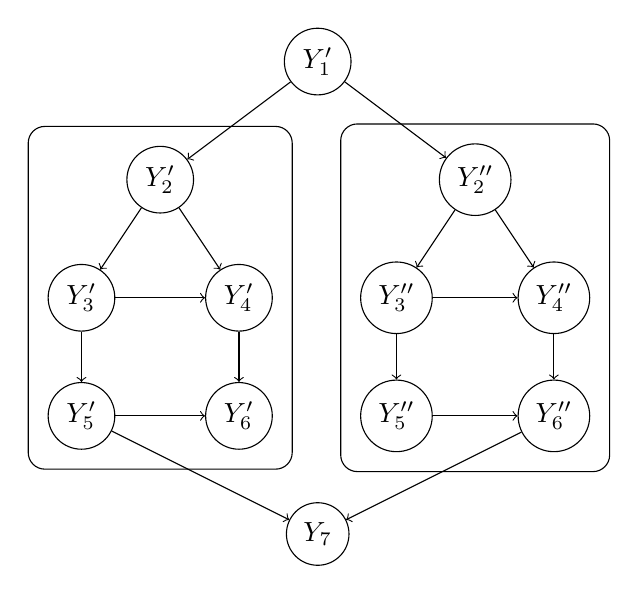
\begin{tikzpicture}[node distance=4cm]
\node[draw,circle] (30) at (3,0) {$Y_1'$};
\node[draw,circle](11) at (1,-1.5) {$Y_2'$};
\node[draw,circle] (51) at (5,-1.5) {$Y_2''$};
\node[draw,circle] (02) at (0,-3) {$Y_3'$};
\node[draw,circle] (22) at (2,-3) {$Y_4'$};
\node[draw,circle] (42) at (4,-3) {$Y_3''$};
\node[draw,circle] (62) at (6,-3) {$Y_4''$};
\node[draw,circle] (03) at (0,-4.5) {$Y_5'$};
\node[draw,circle](23) at (2,-4.5) {$Y_6'$};
\node[draw,circle](43) at (4,-4.5) {$Y_5''$};
\node[draw,circle] (63) at (6,-4.5) {$Y_6''$};
\node[draw,circle] (34) at (3,-6) {$Y_7$};
\draw[->] (30) -- (11);
\draw[->] (30) -- (51);
\draw[->] (11) -- (02);
\draw[->] (11) -- (22);
\draw[->] (51) -- (42);
\draw[->] (51) -- (62);
\draw[->] (02) -- (22);
\draw[->] (02) -- (03);
\draw[->] (22) -- (23);
\draw[->] (42) -- (62);
\draw[->] (42) -- (43);
\draw[->] (62) -- (63);
\draw[->] (63) -- (34);
\draw[->] (03) -- (34);
\draw[->] (03) -- (23);
\draw[->] (43) -- (63);
\node[draw=black, rounded corners=6pt, inner sep =7pt, fit=(11) (03) (23)] {};
\node[draw=black, rounded corners=6pt, inner sep =7pt, fit=(51) (43) (63)] {};
\end{tikzpicture}}
\end{center}
\subcaption{Example of a Bayesian network with identical subnetworks. \label{fig:BNwithsubs}}
\end{minipage}
\begin{minipage}[b]{0.33\linewidth}
\begin{center}
\scalebox{0.8}{
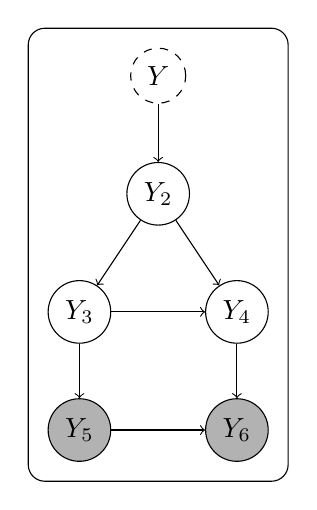
\begin{tikzpicture}[node distance=4cm]
\node[draw,circle,dashed] (10) at (1,0) {$Y$};
\node[draw,circle] (11) at (1,-1.5) {$Y_2$};
\node[draw,circle] (02) at (0,-3) {$Y_3$};
\node[draw,circle] (22) at (2,-3) {$Y_4$};
\node[draw,circle,fill = black!30!white] (03) at (0,-4.5) {$Y_5$};
\node[draw,circle,fill = black!30!white] (23) at (2,-4.5) {$Y_6$};
\draw[->] (10) -- (11);
\draw[->] (11) -- (02);
\draw[->] (11) -- (22);
\draw[->] (02) -- (22);
\draw[->] (02) -- (03);
\draw[->] (22) -- (23);
\draw[->] (03) -- (23);
\node[draw=black, rounded corners=6pt, inner sep =7pt, fit=(10) (03) (23)] {};
\end{tikzpicture}}
\end{center}
\subcaption{Class definition for the subnetworks of Figure \ref{fig:BNwithsubs}. \label{fig:class}}
\end{minipage}
\caption{Example of object orientation in Bayesian networks. \label{fig:objectorient}}
\end{figure}

Considering again the network in Figure \ref{fig:BNwithsubs}, each subnetwork within the rectangles in the object oriented paradigm is an instantiation of  a \textit{class}, called \textit{object}. Figure \ref{fig:class} shows the class definition for the repeated subnetworks of Figure \ref{fig:BNwithsubs}. Each class consists of three types of vertices:
\begin{itemize}
\item input vertices: not true random variables, but artificial nodes that serve as \lq{p}laceholders\rq{.} In Figure \ref{fig:class} the input vertex is the dashed node $Y$ which must have the same state space of $Y_1$;
\item encapsulated vertices: vertices that are hidden outside of the class and that are used only within the class. In Figure \ref{fig:class} the encapsulated vertices are $Y_2$, $Y_3$ and $Y_4$;
\item output vertices: part of the class that is accessible from outside and that can be connected to other classes. The output vertices of the class in Figure \ref{fig:class} are the shaded nodes $Y_5$ and $Y_6$. 
\end{itemize}
Encapsulated and output vertices are allowed to be objects, whilst input vertices must be variables. 

Given the class definition in Figure \ref{fig:class}, we can represent the BN of Figure \ref{fig:BNwithsubs} as the OOBN reported in Figure \ref{fig:OOBN}.  In this network the encapsulated vertices are hidden and only input and output nodes of the class explicitly appear. Each rectangle is an object and in each object the relative output nodes are connected to elements external to the class. The dashed arrows into the input node indicate which node $Y$ is a placeholder for (in this case $Y_1$ for both objects).

Even in this simple example the expressive power of OOBNs becomes apparent, modularising the overall problem in different layers formally separated. Of course in much larger examples OOBNs provide an even more compact representation of the domain under consideration: see for example \citet{Neil2000}.

\begin{figure}
\vspace{-0.1cm}
\begin{center}
\scalebox{0.8}{
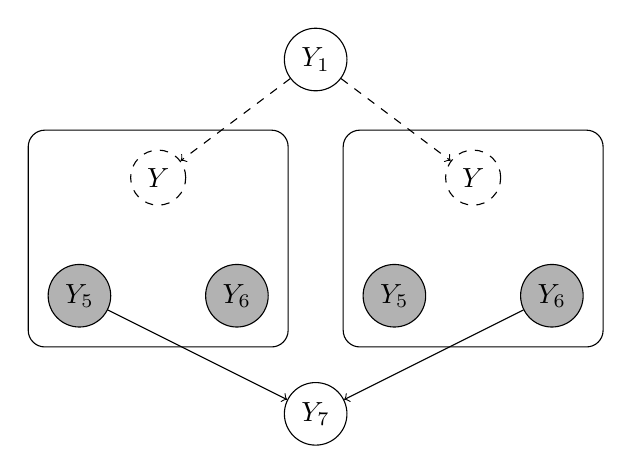
\begin{tikzpicture}[node distance=4cm]
\node[draw,circle] (30) at (3,0) {$Y_1$};
\node[draw,circle,dashed](11) at (1,-1.5) {$Y$};
\node[draw,circle,dashed] (51) at (5,-1.5) {$Y$};
\node[draw,circle,fill = black!30!white] (03) at (0,-3) {$Y_5$};
\node[draw,circle,fill = black!30!white](23) at (2,-3) {$Y_6$};
\node[draw,circle,fill = black!30!white](43) at (4,-3) {$Y_5$};
\node[draw,circle,fill = black!30!white] (63) at (6,-3) {$Y_6$};
\node[draw,circle] (34) at (3,-4.5) {$Y_7$};
\draw[dashed,->] (30) -- (11);
\draw[dashed,->] (30) -- (51);
\draw[->] (03) -- (34);
\draw[->] (63) -- (34);
\node[draw=black, rounded corners=6pt, inner sep =7pt, fit=(11) (03) (23)] {};
\node[draw=black, rounded corners=6pt, inner sep =7pt, fit=(51) (43) (63)] {};
\end{tikzpicture}}
\end{center}
\vspace{-0.3cm}
\caption{Object oriented representation of the Bayesian network of Figure \ref{fig:BNwithsubs}, whose class is defined in Figure \ref{fig:class}. \label{fig:OOBN}}
\end{figure}

\subsubsection{Probabilistic Undirected Graphs.}
We now consider probability densities $f$ that can be described by an Undirected Graph (UG) $\Gr$. These are used in particular when there is no clear directional relationships between the variables under study. For the purpose of the thesis we assume $\Gr$ to be always decomposable in the undirected case: we  motivate this assumption below. Just as in the directed case of Section \ref{sec:BN}, we first introduce a class of densities which are in some sense compatible to the graph and then define the class of UG models called \textit{Markov Networks (MNs)}. References about these models are countless \citep[see e.g.][]{Lauritzen1996a, Cowell1999a, Castillo1997b}. We follow here \citet{Dawid1993}.

\begin{definition}
Let $A,B\subset[n]$ and $V(\Gr)=\{Y_i: i\in[n]\}$ be the vertex set of an UG $\Gr$. A density $f$ over $\bm{Y}\;|\;\bm{\theta}$ is called \emph{Markov} if, for any decomposition $\{Y_i:i\in A\}$, $\{Y_i:i\in B\}$ of $\Gr$,
$\bm{Y}_A\independent \bm{Y}_B \;|\; \bm{Y}_{A\cap B},\bm{\theta}$
\end{definition}

\begin{definition}
A decomposable MN model consists of a decomposable UG $\Gr$ with vertex set $\{Y_i:i\in[n]\}$ together with a Markov density $f$. 
\end{definition}
Note that for each vertex $Y_i$ of an MN, the conditional independence statement
\begin{equation*}
\label{eq:independenceUG}
Y_i\independent \bm{Y}_{[n]\setminus \{i\}}\;|\; \bm{Y}_{Ne_i},\bm{\theta},
\end{equation*}
holds, where $Ne_i$ is the index set of the neighbours of $Y_i$. Thus, just as  in the directed case, Markov densities associated to a (decomposable) UG are the only ones entertaining the separations implied by the graph. In order to deduce the associated Markov factorisation as in the directed case, we first need to introduce the notion of \textit{consistency}.
\begin{definition}
Let $f_A$ and $f_B$ be densities over $\bm{Y}_A\;|\;\bm{\theta}$ and $\bm{Y}_B\;|\;\bm{\theta}$ respectively, $A,B\in[n]$. We say that $f_A$ and $f_B$ are consistent if they both yield the same density over $\bm{Y}_{A\cap B}\;|\;\bm{\theta}$. 
\end{definition}
Now letting $\mathcal{C}$ and $\mathcal{S}$ be the sets of the indices of the cliques and the separators respectively of an UG $\Gr$, we have the following.
\begin{lemma}
\label{lemma:Markov}
The unique Markov density $f$ over a decomposable UG $\Gr$ having \emph{consistent} densities as its clique marginals factorises as
\begin{equation*}
\label{eq:UGmarkovfactorization}
f(\bm{y}\;|\;\bm{\theta})=\frac{\prod_{C\in\mathcal{C}}f(\bm{y}_C\;|\;\bm{\theta}_C)}{\prod_{S\in\mathcal{S}}f(\bm{y}_S\;|\; \bm{\theta}_S)^{v_S}},
\end{equation*}
where $v_S$ is the multiplicity of the separator $S$, $\bm{\theta}_C$, $\bm{\theta}_S$ are the parameter vectors associated to $\bm{Y}_C$ and $\bm{Y}_S$, respectively, and $\mathcal{C}$ and $\mathcal{S}$ are the index sets of the cliques and the separators, respectively.
\end{lemma} 

Given an order over the elements of $\mathcal{C}$ exhibiting the running intersection property (see Appendix \ref{appendixB}), the density of a Markov density over a decomposable graph can be alternatively written as, assuming the graph includes $m$ cliques,
\begin{equation*}
\label{eq:cliquesfactorization}
f(\bm{y}\;|\;\bm{\theta})=\prod_{i\in[m]_1} f(\bm{y}_{R_i}\;|\; \bm{y}_{S_i}, \bm{\theta}_{R_i})f(\bm{y}_{C_1}\;|\;\bm{\theta}_{C_1}),
\end{equation*}
where $R_i=C_i\setminus S_i$.

\begin{figure}
\vspace{-0.3cm}
\begin{center}
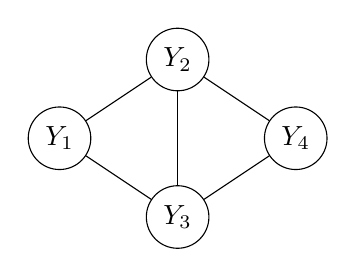
\begin{tikzpicture}
\node[draw,circle] (01) at (0,-1) {$Y_1$};
\node[draw,circle]  (10) at (1.5,0) {$Y_2$};
\node[draw,circle]   (12) at (1.5,-2) {$Y_3$};
\node[draw, circle]  (21) at (3,-1){$Y_4$};
\draw[-] (01) -- (10);
\draw[-] (01) -- (12);
\draw[-] (10) -- (12);
\draw[-] (21) -- (10);
\draw[-] (21) -- (12);
\end{tikzpicture}
\end{center}
\vspace{-0.4cm}
\caption{Example of a decomposable undirected graph with four vertices. \label{fig:UG}}
\end{figure}

\begin{example}
Consider the UG  with vertex set $\{Y_1,Y_2,Y_3,Y_4\}$ in Figure \ref{fig:UG}. The conditional independence statement associated to this graph is $
\ci{Y_4}{Y_1}{Y_2,Y_3,\bm{\theta}}$,
and therefore the associated density factorises as
\begin{equation*}
\label{eq:UGexamplefactorization}
f(\bm{y}\;|\;\bm{\theta})=\frac{f(y_1,y_2,y_3\;|\; \bm{\theta}_{[3]})f(y_2,y_3,y_4\;|\; \bm{\theta}_{[4]_1})}{f(y_2,y_3\;|\; \bm{\theta}_{[3]_1})},
\end{equation*}
or alternatively as 
\[
f(\bm{y}\;|\;\bm{\theta})=f(y_4\;|\; y_2,y_3, \bm{\theta}_4)f(y_1,y_2,y_3\;|\; \bm{\theta}_{[3]})=f(y_1\;|\; y_2,y_3, \bm{\theta}_1)f(y_2,y_3,y_4\;|\; \bm{\theta}_{[4]_1}).
\]
\end{example}

Just as in the directed case, conditions over the parameter vector can be imposed entailing distributed  inferences. For the purpose of this thesis we introduce only the strong hyper Markov condition of \citet{Dawid1993}.
\begin{definition}
\label{def:strongMarkov}
A density $\pi$ is strong hyper Markov for $\Gr$ if, for any decomposition $\{Y_i:i\in A\}$, $\{Y_i:i\in B\}$ of $\Gr$, $\bm{\theta}_A\independent \bm{\theta}_B$.
\end{definition} 
Since the cliques of a decomposable UG can be ordered to sequentially form a decomposition, we have the following result from \citet{Dawid1993}.
\begin{lemma}
\label{lemma:strongMarkov}
If a density $\pi$ for $\bm{\theta}$ is strong hyper Markov  then 
$
\pi(\bm{\theta})=\prod_{C\in\mathcal{C}}\pi(\bm{\theta}_{C}).$
\end{lemma}
We do not show in detail how to build a distribution exhibiting the strong hyper Markov condition. However we briefly note here that this can be straightforwardly done by considering the Markov combinations  of the marginal distributions over the cliques of the graph \citep{Massa2010}. 

The following proposition from \citet{Dawid1993} then shows how the strong hyper Markov condition is associated to fast distributed Bayesian inference.
\begin{proposition}
\label{prop:markovupdating}
Assume a vector $\bm{X}$ is sampled from the same population of $\bm{Y}$ and assume the density $\pi$ of $\bm{\theta}$ is strong hyper Markov. Then, the posterior distribution obtained by conditioning on the complete data $\bm{X}=\bm{x}$ is the unique strong hyper Markov distribution specified by the clique-marginal prior distributions given by $
\pi(\bm{\theta}_C\;|\; \bm{x})=f(\bm{x}_C\;|\;\bm{\theta}_C)\pi(\bm{\theta}_C).$
\end{proposition}
Therefore Bayesian updating can be performed locally within each clique whilst retaining the strong hyper Markov condition. Note that  the above result does not hold in general for non-decomposable undirected models. Whilst global independence is retained after observing certain incomplete datasets, strong hyper Markov laws are also broken by any incomplete observation. In Chapter \ref{chapter3} however we are able to show that for certain sets of incomplete observation the strong hyper Markov property can be retained if Bayesian updating is performed simultaneously for all the elements of this set.

We now consider the class of MN models whose associated distribution is Gaussian. A \emph{Gaussian MN} with decomposable UG $\Gr$, $V(\Gr)=\{Y_i:i\in[n]\}$, is defined as $\bm{Y}\;|\;\bm{\mu},\Sigma\sim \N(\bm{\mu},\Sigma)$, where $\bm{\mu}=(\mu_i)^\T_{i\in[n]}\in\mathbb{R}^n$ and $\Sigma$ is an $n\times n$ covariance matrix\footnote{A covariance matrix is a symmetric positive semidefinite matrix with entries in $\mathbb{R}_{>0}$ on the diagonal and in $\mathbb{R}$ otherwise.} such that if $(Y_i,Y_j)\not\in E(\Gr)\Longrightarrow \Sigma_{ij}^{-1}=0$, where $\Sigma_{ij}^{-1}$ is the entry of $\Sigma^{-1}$ in position $(i,j)$. So for example the covariance matrix associated to the Gaussian MN with graph in Figure \ref{fig:UG} is such that its inverse has zero entries in positions $(1,4)$ and $(4,1)$. Now for simplicity let $\bm{\mu}=\bm{0}$. Such a model class is usually referred to as a covariance selection model \citep{Wermuth1976}. Recall from Appendix \ref{sec:niw} that the Inverse Wishart distribution allows for conjugate learning with Normal models when defined as a prior of the covariance matrix. Let $\Sigma\sim \IW(A,d)$, where $A$ is a positive semidefinite $n\times n$ matrix and $d\in\mathbb{Z}_{\geq n}$. It is well known that for a subset $B\in[n]$, $\bm{Y}_{B}\sim \N(\bm{0},\Sigma_{B,B})$ and $\Sigma_{B,B}\sim \IW(A_{B,B},d)$, where, for a matrix $\Sigma$, $\Sigma_{B,B}$ is its submatrix with rows and columns $i\in B$ \citep[see e.g.][]{Dawid1993}. For every clique $C\in\mathcal{C}$ of $\Gr$, let $\bm{Y}_{C}\;|\;\Sigma_{C,C}\sim \N(\bm{0},\Sigma_{C,C})$ and assume the covariance  $\Sigma_{C,C}$ has an Inverse Wishart prior distribution $\IW(A^C,d)$. A unique strong hyper Markov distribution for the whole graph $\Gr$ having as marginals over the cliques these Inverse Wishart distributions exists if, calling $S_{ij}=C_i\cap C_j$, the matrices $A^{C_i}_{S_{ij},S_{ij}}$ and $A^{C_j}_{S_{ij},S_{ij}}$ are identical.\footnote{This result follows from Proposition 5.9 of \citet{Dawid1993} which we have not introduced here since it would require the introduction of additional concepts not relevant for the thesis. In a nutshell, this result is true because the Inverse Wishart is conjugate for the Normal covariance selection model and this distribution is a member of the exponential family.} We then say that $\Sigma$ follows an hyper Inverse Wishart distribution with parameters $A$ and $d$, $\Sigma\sim \HIW(A,d)$, where $A$ is such that $A_{C,C}=A^C$, for $C\in\mathcal{C}$.  

For the graph in Figure \ref{fig:UG}, let  $\Sigma_{[3],[3]}\sim \IW(A^{123},d)$ and $\Sigma_{[4]_1,[4]_1}\sim \IW(A^{234},d)$. Then an hyper Inverse Wishart distribution for this graph having this marginals exists if $A^{234}_{[3]_1,[3]_1}=A^{123}_{[3]_1,[3]_1}$.

Suppose now that a vector of observations $\bm{x}=(\bm{x}^\T_i)^\T_{i\in[m]}$ from the same family of $\bm{Y}$ has been collected, where $\bm{x}_i=(x_{ij})^\T_{j\in[n]}$. Assume an hyper Markov law is constructed from the clique marginals as exemplified above. Then from Appendix \ref{sec:niw} and Proposition \ref{prop:markovupdating} we know that for the covariance selection model the posterior density of $\Sigma\;|\;\bm{x}$ is strong hyper Markov, where each marginal over the submatrix associated with a clique $\Sigma_{C,C}$, $C\in\mathcal{C}$, follows an Inverse Wishart with parameters $A^C+mS_{C,C}$ and $d+m$, where $S$ is equal to $m^{-1}\sum_{i\in[m]}\bm{x}_i\bm{x}_i^\T$ (see Appendix \ref{sec:niw}). This can be easily noted within our example. The marginal posteriors over the cliques are $A^{123}\sim \IW(A^{123}+mS_{[3],[3]},d+m)$ and $A^{234}\sim \IW(A^{234}+mS_{[4]_1,[4]_1},d+m)$. It then holds that $A^{123}_{[3]_1,[3]_1}+mS_{[3]_1,[3]_1}=A^{234}_{[3]_1,[3]_1}+mS_{[3]_1,[3]_1}$, where
\begin{equation}
\label{stica}
mS_{[3]_1,[3]_1}=\left(
\begin{array}{cc}
\sum_{i\in[m]}x_{i2}^2&\sum_{i\in[m]}x_{i2}x_{i3}\\
\sum_{i\in[m]}x_{i2}x_{i3}&\sum_{i\in[m]}x_{i3}^2
\end{array}
\right)
\end{equation} 

\label{sec:UG}
\subsubsection{Probabilistic Chain Graphs.}
\label{sec:PCG}

Probabilistic Chain Graph (PCG) models are a hybrid representation of undirected and directed graphical models, allowing for the underlying graph $\Gr$ to be mixed and more specifically to be a Chain Graph (CG). We give here only a brief introduction to this class of models \citep[see e.g][for more details]{Cowell1999a, Frydenberg1990, Drton2009, Lauritzen1996a}. These are especially useful when there are both directional and non-directional relationships between the variables associated to the vertices of the underlying graph. As with the earlier models, we first introduce the relative Markov property, then derive the associated factorisation and in conclusion define the model. We let $Bd_i$ be the index set of the variables in the boundary of $Y_i$, $i\in[n]$.

\begin{definition}
A probability density $f$ over $\bm{Y}\;|\;\bm{\theta}$ is said to obey the chain Markov property relative to a CG $\Gr$ with vertex set $\{Y_i:i\in [n]\}$  and $m$ strong components if, for every vertex $Y_i$, $i\in[n]$,
$
Y_i\independent \bm{Y}_{A_i'\setminus Bd_i}\;|\; \bm{Y}_{Bd_i},\bm{\theta}$.
\end{definition}


\begin{proposition}
If a density $f$ obeys the chain Markov property relative to a CG $\Gr$ with vertex set $\{Y_i:i\in[n]\}$, then its density factorises as
\begin{equation*}
\label{eq:chainfactorization}
f(\bm{y}\;|\; \bm{\theta})= \prod_{i\in[m]} f\left(\bm{y}_{C_i}\;|\; \bm{y}_{\Pi_{C_i}}, \bm{\theta}_{C_i}\right),
\end{equation*}
where $C_1,\dots,C_m$ are the index sets of the variables in the strong components of $\Gr$ and $\Pi_{C_i}=\cup_{j\in C_i}\Pi_j$. 
\end{proposition}


We are now ready to formally define the model.
\begin{definition}
A PCG model consists of a CG $\Gr$ together with a density $f$ respecting the chain Markov property. 
\end{definition} 

\begin{figure}
\vspace{-0.2cm}
\begin{center}
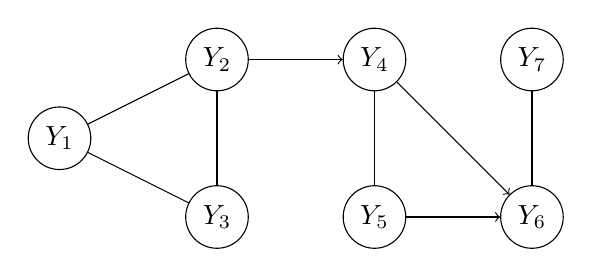
\begin{tikzpicture}
\node[draw,circle] (01) at (-1,-1) {$Y_1$};
\node[draw,circle] (10) at (1,0) {$Y_2$};
\node[draw,circle] (12) at (1,-2) {$Y_3$};
\node[draw,circle] (20) at (3,0) {$Y_4$};
\node[draw,circle] (22) at (3,-2) {$Y_5$};
\node[draw,circle] (32) at (5,-2) {$Y_6$};
\node[draw,circle] (30) at (5,0) {$Y_7$};
\draw[-] (01) -- (10);
\draw[-] (01) -- (12);
\draw[-] (10) -- (12);
\draw[->] (10) -- (20);
\draw[-] (20) -- (22);
\draw[->] (20) -- (32);
\draw[->]  (22) -- (32);
\draw[-]  (32) -- (30);
\end{tikzpicture}
\end{center}
\vspace{-0.2cm}
\caption{Example of a probabilistic chain graph model. \label{fig:CG}}
\end{figure}

\begin{figure}
\vspace{-0.2cm}
\begin{center}
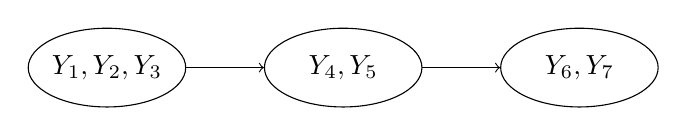
\begin{tikzpicture}
\node[draw,ellipse, minimum height=1cm, minimum width=2cm,inner sep=0pt] (00) at (0,0) {$Y_1, Y_2,Y_3$};
\node[draw,ellipse, minimum height=1cm, minimum width=2cm,inner sep=0pt] (10) at (3,0) {$Y_4, Y_5$};
\node[draw,ellipse,minimum height=1cm, minimum width=2cm,inner sep=0pt](20) at (6,0) {$Y_6, Y_7$};
\draw[->] (00) -- (10);
\draw[->] (10) -- (20);
\end{tikzpicture}
\end{center}
\vspace{-0.4cm}
\caption{Representation of the chain graph in Figure \ref{fig:CG} as a directed acyclic graph. \label{fig:CGDAG}}
\end{figure}


\begin{example}
Consider the PCG in Figure \ref{fig:CG}. It can be deduced from this graph that the following conditional independence statements need to hold for a chain Markov distribution
\begin{equation*}
\begin{array}{lccl}
Y_4\independent Y_1,Y_3\;|\; Y_2,Y_5,\bm{\theta},&&& \ci{Y_5}{Y_1,Y_2,Y_3}{Y_4,\bm{\theta}}, \\
 Y_6\independent Y_1,Y_2,Y_3\;|\; Y_4,Y_5,Y_7,\bm{\theta},&&& \ci{Y_7}{Y_1,\dots,Y_5}{Y_6,\bm{\theta}},
\end{array}
\label{eq:examplechainindependence}
\end{equation*}
and the associated density can be factored as
\begin{equation*}
\label{eq:chainexamplefactorization}
f(\bm{y}\;|\; \bm{\theta})=f(y_6,y_7\;|\; y_4,y_5, \bm{\theta}_{67})f(y_4,y_5\;|\; y_3, \bm{\theta}_{45})f(y_1,y_2,y_3\;|\;\bm{\theta}_{123}).
\end{equation*}
\end{example}

Note that each PCG can be represented by a less expressive DAG whose vertex set corresponds to the strong components of the underlying CG. So for example the PCG in Figure \ref{fig:CG} can be transformed into the DAG of Figure \ref{fig:CGDAG}.
 
\subsubsection{Staged and Event Trees.}
\label{sec:tree}
All the classes of models defined so far are able  to depict standard conditional independence statements only. The class of \textit{event tree} models we discuss in this section is able to explicitly represent context specific independences. Event trees are such that their nodes are the situations in which a process might find itself and the edges emanating from a node are the possible unfoldings given the current situation. It has been extensively discussed in the literature that these models are extremely expressive in describing how processes might unfold. These are  especially useful in the cases where the variables are ordered in a way that follows the narrative of the events \citep{Shafer1996, Freeman2011, Smith2010}. 
 
Let $\mathcal{T}$ be a directed tree, $\Lambda(v,\mathcal{T})$ denote the set of paths from $v\in V(\mathcal{T})$ to a leaf node of $\mathcal{T}$ and $\mathcal{Y}=\Lambda(s_0,\mathcal{T})$, where $s_0$ is the root of the tree, be the set of root-to-leaf paths. Each path $y\in\mathcal{Y}$ is a so-called atomic event, i.e. a possible unfolding of events. Finally let $\mathcal{Y}_s$ denote the set of children of a situation $s\in S(\mathcal{T})$. 

\begin{definition}
An \textbf{event tree} is a directed tree $\mathcal{T}$ together with a random variable $Y_s$ for each situation $s\in S(\mathcal{T})$ with sample space $\mathcal{Y}_s$ defined conditional on having reached vertex $s$. The distribution of $Y_s$ is determined by the \emph{floret probability vector} $\bm{\theta}_s=(\theta_{ss'})^\T_{s'\in\mathcal{Y}_s}$, where  $\theta_{ss'}=\mathbb{P}(Y_s=s')$.
\end{definition}

\begin{figure}
\centerline{
\hspace*{-16mm} \xymatrixrowsep{0.5pc}{\xymatrixcolsep{2pc}
\xymatrix{
&&&&\bullet~v_{7}\\
&&&\bullet~v_{3}\ar@[red][r]_{\text{no}}\ar@[blue][ru]^{\text{yes}}&\bullet~v_{8}\\
&&\bullet~v_{1}\ar[r]_{\text{low}}\ar[ru]^{\text{high}}&\bullet~v_{4}\ar@[blue][r]|{\text{yes}}\ar@[red][rd]_{\text{no}}&\bullet~v_{9}\\
v_0\hspace*{-16mm}&\bullet\ar[ru]^{\text{yes}}\ar[rd]_{\text{no}}&&&\bullet~v_{10}\\
&&\bullet~v_{2}\ar[r]^{\text{high}}\ar[rd]_{\text{low}}&\bullet~v_{5}\\
&&&\bullet~v_{6}
}}}
\caption{Example of an event tree on three variables with the additional representation of its stages in different colors. \label{fig:ET}}
\end{figure}

The expressive power of event trees can be increased by identifying probabilities associated to different edges that are equal. Trees can then be embellished by a colouring of the edges, where two edges have same colour if their associated probabilities are equal.

\begin{definition}
A \textbf{staged tree} is an event tree where, for some $s
,s'\in S(\mathcal{T})$, the floret probability vectors are identified, $\bm{\theta}_s=\bm{\theta}_{s'}$, and equally coloured. Then $s$ and $s'$ are in the same \emph{stage}. We let $\mathbb{W}$ be the set of stages of $\mathcal{T}$.
\end{definition}
  

\begin{example}
\label{ex:staged}
Suppose a problem is modelled with three binary random variables: $Y_1$, release from a source term; $Y_2$, level of contamination in the surrounding area; $Y_3$, political disruption in the region due to the release. Suppose $\mathcal{Y}_1=\mathcal{Y}_3=\{\textnormal{yes},\textnormal{no}\}$ and $\mathcal{Y}_2=\{\textnormal{high},\textnormal{low}\}$. It is assumed that, if there has been a release, the level of contamination does not provide any information to predict the political disruption. This problem could then be modelled by a BN with vertex set $\{Y_1,Y_2,Y_3\}$ and edge set $\{(Y_1,Y_2), (Y_1,Y_3)\}$. 

However the BN representation forces us to retain information which is meaningless in this context, as for instance the atom (no,high,yes) which has probability zero. This is on the other hand explicitly modelled in the staged tree in Figure \ref{fig:ET}. In this tree the leftmost two edges are the possible outcomes of $Y_1$, the edges in the center are the outcomes of $Y_2$ given the different levels of $Y_1$, whilst the rightmost edges coincide with the outcomes of $Y_3$ given $Y_2$ and $Y_1$. In the lower part of the tree, associated to $Y_1=\textnormal{no}$, there are no outcomes for the political disruption variable, as these have probability zero. The set of situations of this tree includes vertices $\{v_0,\dots, v_6\}$ and leaves $\{v_{7},\dots, v_{10}\}$. Its stages are $w_0=\{v_0\}$, $w_1=\{v_1\}$, $w_2=\{v_2\}$, $w_3=\{v_3,v_4\}$. Furthermore $\mathbb{W}=\{w_0,\dots,w_3\}$. The tree representation of the associated BN model is in Figure \ref{fig:ETBN}. Such a tree is extremely regular in its colouring and each of its root to leaf paths have the same length: a property exhibited by the tree representation of any BN (see for more details Section \ref{sec:diff}).
\end{example}

\begin{figure}
\centerline{
\hspace*{-16mm} \xymatrixrowsep{0.5pc}{\xymatrixcolsep{2pc}
  \xymatrix{
&&&&\bullet~v_{7}\\
&&&\bullet~v_{3}\ar@[red][r]_{\text{no}}\ar@[blue][ru]^{\text{yes}}&\bullet~v_{8}\\
&&\bullet~v_{1}\ar[r]_{\text{low}}\ar[ru]^{\text{high}}&\bullet~v_{4}\ar@[blue][r]|{\text{yes}}\ar@[red][rd]_{\text{no}}&\bullet~v_{9}\\
v_0\hspace*{-16mm}&\bullet\ar[ru]^{\text{yes~}}\ar[rdd]_{\text{no}}&&&\bullet~v_{10}\\%
&&&&\bullet~v_{11}\\
&&\bullet~v_{2}\ar[rd]_{\text{low}}\ar[r]^{\text{high}}&\bullet~v_{5}\ar@[green][r]_{\text{no}}\ar@[brown][ru]^{\text{yes}}&\bullet~v_{12}\\
&&&\bullet~v_{6}\ar@[brown][r]|{\text{yes}}\ar@[green][rd]_{\text{no}}&\bullet~v_{13}\\
&&&&\bullet~v_{14}\\
}}}
\caption{Tree representation of the Bayesian network of Example \ref{ex:staged} .\label{fig:ETBN}}
\end{figure}

Although the colouring of the edges entails an improved representation of the overall structure of the problem at hand, conditional independences are still difficult to read from the graph. In addition as the number of variables increases, the size of the tree becomes quickly too large to be concisely reported. The class of models we introduce in the following section is able to compactly represent every conditional independence entertained.

\subsubsection{Chain Event Graphs.}
\label{sec:CEG}

Chain Event Graphs (CEGs) \citep{Smith2008} are models capable of representing context specific conditional independences in a single compact graphical representation. CEGs are constructed by starting with a staged tree, therefore requiring variables to be discrete, and then merging into a single vertex certain situations that are in the same stage. 

\begin{definition}
We say that two situations $s$ and $s'$ are in the same \emph{position} if the subtrees with roots $s$ and ${s'}$, respectively, have the same topology and the same edge colouring. We let $\mathbb{B}$ denote the set of positions of a staged tree.
\end{definition}

Note that two situations in the same position are by definition also in the same stage, whilst it does not necessary follows that two situations in the same stage are also in the same position. 

\begin{example}
 Considering the staged tree in Figure \ref{fig:ET}, we can see that for this example the set of stages coincides with the one of positions. 
\end{example} 
 
 \begin{definition}
 A \textbf{CEG} is the graph obtained by collapsing a staged tree into its positions. Its vertex set is equal to $\{\mathbb{B}\cup b_{\infty}\}$, where $b_{\infty}$ is the vertex collecting all the leaves of the tree. Its edge set is such that 
 \begin{itemize}
 \item there is an edge $(b_i,b_j)$, $b_i,b_j\in\mathbb{B}$, for every edge from a generic vertex $v\in b_i$ to any vertex $v'\in b_j$;
 \item there is an undirected edge between any two positions in the same stage;
 \end{itemize}
 \end{definition} 
 
\begin{example}
 The CEG representation of the staged tree of Figure \ref{fig:ET} is shown in Figure \ref{fig:CEG}, where we further annotated and coloured the edges as in \citet{Barclay2013a}. 
 \end{example}
 
\begin{figure}
\vspace{-.3cm}
\begin{center}
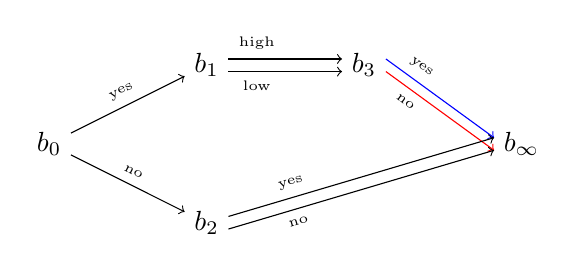
\begin{tikzpicture}
\node (00) at (0,0) {$b_0$};
\node (1-1) at (2,-1) {$b_2$};
\node (11) at  (2,1) {$b_1$};
\node (21) at (4,1) {$b_3$};
\node (30) at (6,0) {$b_{\infty}$};
\draw[->,sloped, anchor=center, above] (00) to  node {\tiny{yes}} (11);
\draw[->,sloped, anchor=center, above] (00) to  node {\tiny{no}} (1-1);
\draw[->,sloped, anchor=center, above,near start] ([yshift=0.08cm]11.east) to  node {\textcolor{black}{\tiny{high}}} ([yshift=0.08cm]21.west);
\draw[->,sloped, anchor=center, below,near start] ([yshift=-0.08cm]11.east) to  node {\textcolor{black}{\tiny{low}}} ([yshift=-0.08cm]21.west);
\draw[->,blue,sloped, anchor=center, above,near start] ([yshift=0.08cm]21.east) to  node {\textcolor{black}{\tiny{yes}}} ([yshift=0.08cm]30.west);
\draw[->,red,sloped, anchor=center, below,near start] ([yshift=-0.08cm]21.east) to  node {\textcolor{black}{\tiny{no}}} ([yshift=-0.08cm]30.west);
\draw[->,sloped, anchor=center, above,near start] ([yshift=0.08cm]1-1.east) to  node {\textcolor{black}{\tiny{yes}}} ([yshift=0.08cm]30.west);
\draw[->,sloped, anchor=center, below,near start] ([yshift=-0.08cm]1-1.east) to  node {\textcolor{black}{\tiny{no}}} ([yshift=-0.08cm]30.west);
\end{tikzpicture}
\end{center}
\vspace{-.5cm}
\caption{A chain event graph model representing the staged tree in Figure \ref{fig:ET}. \label{fig:CEG}}
\end{figure}

We chose the CEG as a representative model for context specific independences for two main reasons. First, compared to other models capable of  representing context specific conditional independences,  the CEG consists of a single graph. Furthermore   \citet{Smith2008} showed that every discrete BN can be represented as a CEG, whilst the converse does not hold. This is not case for example for probabilistic decision graphs \citep{Jaeger2004} and context specific BNs \citep{Boutilier1996}. \citet{Barclay2013a} nicely discussed how to convert a BN into a CEG model and how to measure the advantages of the latter representation. Second, a wide range of methods to perform various statistical analyses have been developed for this model class \citep[see e.g.][]{Barclay2013a,Barclay2014, Freeman2011, Thwaites2010, Thwaites2015}.

Importantly, under assumptions similar to local and global independence, but customised to staged trees and CEGs, Bayesian updating can be performed in a distributed way through the Multinomial-Dirichlet recursions illustrated in Appendix \ref{sec:multidir}. In Chapter \ref{chapter3} we generalise these independences for CEGs to take into account that probabilities over the graph are elicited by different groups of experts.  Suppose $w_i\in\mathbb{W}$ has $n_i$ emanating edges with associated probability vector $\bm{\theta}_i=(\theta_{ij})^\T_{j\in[n_i]}$, such that $\theta_{ij}\in(0,1)$ and $\sum_{j\in[n_i]}\theta_{ij}=1$, $j\in[n_i]$, $i\in[n]$. For a random sample $\bm{x}^\T=(\bm{x}_i^\T)_{i\in[n]}$, where $\bm{x}_i=(x_{ij})^\T_{j\in[n_i]}$ is the vector of the number of units that starts at stage $w_i$ and go through the emanating edges, it holds that
\begin{equation}
\label{eq:liktree}
f(\bm{x}\;|\;\bm{\theta})\propto\prod_{i\in[n]}\prod_{j\in[n_i]}\theta_{ij}^{x_{ij}},
\end{equation}
where we further assumed that $\bm{x}_i\independent \bm{x}_j\;|\;\bm{\theta}$, $i,j\in[n]$, and $\bm{\theta}^\T=(\bm{\theta}_i^\T)_{i\in[n]}$. Therefore the likelihood is multinomial. Now assuming $\bm{\theta}$ has mutually independent parameters, the independence  is retained a posteriori when the prior distribution is updated with the likelihood in equation (\ref{eq:liktree}). In particular this is conjugate if each stage probability vector $\bm{\theta}_i$ is given a Dirichlet prior distribution with parameter $\bm{a}_i=(a_{ij})^\T_{j\in[n_i]}\in\mathbb{R}^{n_i}_{>0}$. The posterior is then again Dirichlet with parameter $\bm{a}_i+\bm{x}_i$. \citet{Freeman2011} proved that assuming mutual independence of the parameters and some other fairly mild conditions, the prior distribution is necessarily Dirichlet.

\subsection{Dynamic Models}
\label{sec:dynmod}
In this section we deal with models for processes that are observed at several points in time, usually called \emph{time series}. The graphical models presented so far correspond to a fixed time, but now the random variables associated to the vertices of these will be allowed to vary in time, whilst, in most cases, the structure of the underlying graphical representation will remain constant through time. Such models allow for enough flexibility to represent situations where the relevant factors vary through time.

 Let $\{\bm{Y}_t\}_{t\in[T]}=\{Y_i(t):i\in[n]\}_{t\in[T]}$ be a $n$-dimensional time series with finite time horizon $T$, where $\{Y_i(t)\}_{t\in[T]}$, $i\in[n]$, is a univariate time series. We let $\mathcal{Y}_i$ and $\bm{\mathcal{Y}}=\bigtimes_{i\in[n]}\mathcal{Y}_i$ be the sample spaces of  $Y_i(t)$ and $\bm{Y}(t)$ respectively, for any $t\in[T]$. The density function of a generic $Y_i(t)$ is parametrised by  $\bm{\theta}_i(t)$ with sample space $\bm{\Theta}_i$. Let $\bm{Y}_A(t)^\T=(Y_i(t))_{i\in A}$, $\bm{Y}_A^t=(\bm{Y}_A(1)^\T,\dots,\bm{Y}_A(t)^\T )^\T$, $\bm{Y}_{[n]}(t)=\bm{Y}(t)$ and $\bm{\theta}_A^t=(\bm{\theta}_A(1)^\T,\dots, \bm{\theta}_A(t))^\T$, $A\subseteq[n]$. We denote with lower case letters instantiations of these random variables and vectors, and for any $t\in[T-1]$ the sample space of $(\bm{Y}(t),\bm{Y}(t+1))$ is $\bm{\mathcal{Y}}\bigtimes \bm{\mathcal{Y}}$. Finally, we denote with $I^t$ the information set at time $t$, which includes all the relevant information available to the DM. We assume in this section that $I^t=\{I^{t-1},\bm{Y}(t-1)\}$, $t\in[T]_1$.

\subsubsection{Dynamic Linear Models.}
\label{sec:DLM}
Based on a distributed version of the Kalman Filter \citep{Kalman1960}, the theory of Dynamic Linear Models (DLMs) was introduced in \citet{Harrison1976} and described in the seminal book of \citet{West1997}. This theory allows for a coherent updating of probabilities in dynamic frameworks, which can be then embedded within the graphical models we introduce in the following sections. The key property of such models is the underlying conditional independence structure which assumes that at each time point all the relevant evidence  is summarised in the distribution $\bm{\theta}(t)\;|\;\bm{\theta}(t{-1})$, where $\bm{\theta}(t)^\T=(\bm{\theta}_i(t)^\T)_{i\in[n]}$ has dimension $r$, and that consequently all the relevant information to predict $\bm{Y}(t)$ is synthesised in the distribution of $\bm{\theta}(t)$. This is depicted in Figure \ref{fig:CIDLM} implying, for each $t\in [T-1]_1$, $
\ci{\bm{Y}(t)}{I^{t-1}, \bm{\theta}^{t-1}}{\bm{\theta}(t)},$ and  $\ci{\bm{\theta}(t)}{I^{t-1}}{\bm{\theta}(t-1)}$.
 
\begin{figure}
\vspace{-.2cm}
\centerline{
\xymatrix{
&\bm{Y}(t-1)&\bm{Y}(t)&\bm{Y}(t+1)&\\
\ar[r]&\bm{\theta}(t-1)\ar[u]\ar[r]&\bm{\theta}(t)\ar[r]\ar[u]&\bm{\theta}(t+1)\ar[u]\ar[r]&
}}
\caption{Conditional independence structure underlying the dynamic linear model class. \label{fig:CIDLM}}
\end{figure} 

We now introduce the general form of the Normal DLM. 

\begin{definition}
\label{def:DLM}
The \emph{general Normal DLM} is defined by the following three equations.
\begin{align}
&\bm{Y}(t)=F(t)^{\T}\bm{\theta}(t)+\bm{v}(t),  &\bm{v}(t)&\sim \N\left(\bm{0},V(t)\right),\label{eq:obseq}\\
&\bm{\theta}(t)=G(t)\bm{\theta}(t-1)+\bm{w}(t),  &\bm{w}(t)&\sim \N\left(\bm{0},W(t)\right),\label{eq:evoeq}
\\
&\bm{\theta}(1)\;|\;I^0\sim \N\left(\bm{m}(0),C(0)\right),\nonumber \label{eq:ininfo}
\end{align}
where  $V(t)$, $W(t)$ and $C(0)$ are known covariance matrices of dimensions $n\times n$, $r\times r$ and $r\times r$, respectively, $F(t)$ and $G(t)$ are generic matrices of dimensions $n\times r$ and $r\times r$, respectively, $\bm{m}(0)\in\mathbb{R}^n$ and the errors $\bm{v}(1),\dots,\bm{v}(T), \bm{w}(1),\dots,\bm{w}(T)$ are mutually independent, where $\bm{v}(t)$ and $\bm{w}(t)$, $t\in[T]$, have dimension $n$ and $r$ respectively,  
\end{definition}

Equation (\ref{eq:obseq}) is the \textit{observation equation} specifying the distribution of $\bm{Y}(t)$ conditional on the \textit{system vector} $\bm{\theta}(t)$, having mean $F(t)^{\T}\bm{\theta}(t)$ and variance $V(t)$, also called \textit{observational variance matrix}. The matrix $F(t)$ is referred to as the \textit{regression matrix}, whilst $\bm{v}(t)$ is the \textit{observational error}. Equation (\ref{eq:evoeq}) is the \textit{system evolution equation}, which specifies how the values of the parameter vector evolve trough time. The matrices $G(t)$ and $W(t)$ are called respectively \textit{system transfer} and \textit{system variance} matrices. The vector $\bm{w}(t)$ is called \textit{system error}. 

Note that alternatively the general Normal DLM can be equivalently defined by substituting equations (\ref{eq:obseq})-(\ref{eq:evoeq}) with  the following two conditional distributional specifications:
\begin{equation*}
\label{eq:dlmdefinition}
\bm{Y}(t)\;|\;\bm{\theta}(t)\sim \N\left(F(t)^{\T}\bm{\theta}(t), V(t)\right),\;\;\;\;\;\;\;\; \bm{\theta}(t)\;|\; \bm{\theta}(t{-1}) \sim \N\left(G(t)\bm{\theta}(t-1),W(t)\right).
\end{equation*}

\begin{example}
Special cases of the general Normal DLM model are:
\begin{itemize}
\item a \textit{univariate DLM} is such that $\bm{Y}(t)$ has dimension $1$ (it is therefore a scalar);
\item a \textit{linear univariate DLM} is such that $F(t)=(1,X_{i}(t))_{i\in[r-1]}^\T$, where $X_{i}(t)$ is a regression variable, $i\in [r-1]$;
\item a univariate \textit{regression} DLM is such that the entries of $F(t)$ are generic functions of $X_{1}(t),\dots,X_{r-1}(t)$. 
\end{itemize}
\end{example}

Although we do not focus in this thesis on modelling issues, we note here that the theory of DLMs comprises a large variety of methodologies to model for example both seasonal and polynomial temporal trends. The concept of \textit{discount factors} is also widely used to elicit the values of the observational variance errors. Importantly, the conditional independence structure underlying DLMs provides a natural framework to \textit{intervene} on the system by for example changing the value of some of the model's parameters. This strategy is usually implemented when the model has a poor forecasting performance.

The assumption of Gaussianity in Definition \ref{def:DLM} is not strictly necessary but it entails some computational advantages. Under this assumption the updating equations of the parameters and the observables can be written in closed form and follow a Normal distribution, both in the univariate and the general case. The same property holds for the forecasting distributions, describing the behaviour of the system $k$-steps ahead in the future, for some $k\in\mathbb{Z}_{\geq 1}$. The associated recurrences when variances are known then reduce to the familiar Kalman Filter recurrences.

In practical applications the elicitation of the observational variance is critical and often prohibitive. However, there might be some information regarding its behaviour. Thus in practice $V(t)$ is often assumed unknown and a prior distribution is elicited. In the univariate case, an Inverse Gamma distribution can be given to this error, entailing a conjugate analysis as shown in Appendix \ref{sec:nig}. It is then possible to obtain closed recurrences for both the updating and the forecasting distributions which, unconditionally on V(t), follow a T-distribution (see again Appendix \ref{sec:nig}). Although we have shown in Appendix \ref{sec:niw} a conjugate analysis for the multivariate Normal model, this does not extend straightforwardly in a dynamic setting as in the univariate case to allow for sequential conjugate learning. We note here though that a variety of methods have been developed to approximate both numerically and analytically these recurrences \citep[see][]{West1997}. Most importantly in the following section we introduce a class of multivariate DLMs that entertains exact closed form updating and forecasting routines. 
  
\subsubsection{Multiregression Dynamic Models.}
\citet{Queen1993} introduced the class of \textit{Multiregression Dynamic Models (MDMs)}, multivariate DLMs exhibiting a conditional independence structure between the component time series which remains constant through time.  Although each variable is modelled through a simple univariate regression DLM, where the regressors are specified by the conditional independence structure, the model class of MDMs is in general non Gaussian. The qualitative structure underlying an MDM can be represented through a DAG whose vertices are the component time series. Importantly, the well known BN model we reviewed in Section \ref{sec:BN} is a special case of the MDM.

\begin{definition}
\label{def:MDM}
An \emph{MDM} for the time series $\{\bm{Y}(t)\}_{t\in[T]}$ is defined by a DAG $\Gr$ with vertex set $\{Y^T_i:i\in[n]\}$ together with the following $n$ observation equations, system equation and initial information:
\begin{equation*}
\begin{array}{llc}
Y_i(t)=\bm{F}_i(t)^\T\bm{\theta}_i(t)+v_i(t),&v_i(t)\sim (0,V_i(t)),&i\in[n];\\
\bm{\theta}(t)=G(t)\bm{\theta}(t-1)+\bm{w}(t)&\bm{w}(t)\sim(0,W(t));&\\
\bm{\theta}(0)\;|\; I^0\sim (\bm{m}(0),C(0)).
\end{array}
\end{equation*}

The system vector is $\bm{\theta}_i(t)\in\mathbb{R}^{r_i}$  and $\bm{F}_i(t)$, of dimension $r_i$, is an arbitrary function of $\bm{y}^t_{\Pi_i}$ and $\bm{y}^{t-1}_i$, but  not $\bm{y}^t_{De_i}$ and $y_i(t)$.  The scalar observation variances  $V_i(t)\in\mathbb{R}_{>0}$, $i\in[n]$, can be either known or unknown. The $r\times r$ matrices, $r=\sum_{i=1}^n r_i$, $G(t)=\textnormal{blockdiag}(G_1(t),\dots,G_n(t))$,  $W(t)=\textnormal{blockdiag}(W_1(t),\dots,W_n(t))$ and   $C_0=\textnormal{blockdiag}(C_1(0),\dots,C_n(0))$, are assumed known and such that $W_i(t)$ and $C_i(t)$ are covariance matrices, whilst $G_i(t)$ is a generic matrix, all of dimension $s_i\times s_i$, $i\in [n]$.\footnote{$\blockdiag$ denotes a block-diagonal matrix.} The errors $v_1(t),\dots,v_n(t),\bm{w}_1(t),\dots,\bm{w}_n(t)$, where $\bm{w}_i(t)\sim(\bm{0},W_i(t))$, are mutually independent.
\end{definition} 

\begin{example}
Consider a time series $\{\bm{Y}(t)\}_{t\in[T]}=\{Y_1(t),Y_2(t),Y_3(t),Y_4(t)\}_{t\in[T]}$. An MDM having the conditional independence structure depicted by the DAG in Figure \ref{fig:MDM} would have observation equations in which $\bm{F}_1(t)$ is a function of $\bm{y}^{t-1}_1$ and, for $i\in[4]_1$, $\bm{F}_i(t)$ is a function of $y^{t}_{i-1}$ and $y^{t-1}_i$. 
\end{example}

\begin{figure}
\vspace{-.2cm}
\centerline{
\entrymodifiers={++[o][F-]}
\xymatrix{
\bm{Y}^T_1\ar[r]&\bm{Y}^T_2\ar[r]&\bm{Y}^T_3\ar[r]&\bm{Y}^T_4
}
}
\caption{A directed acyclic graph associated to the conditional independence structure of a multiregression dynamic model. \label{fig:MDM}}
\end{figure}

We now report from \citet{Queen1993} two key results associated to MDMs. For ease of notation we assume the observational variances to be known, but these results straightforwardly generalise to the case of unknown observational variances. 

\begin{proposition}
\label{prop:MDM}
For an MDM over a time series $\{Y_i(t):i\in[n]\}_{t\in[T]}$, we have that 
$\independent_{i\in[n]}\bm{\theta}_i(t)\;|\; \bm{y}^{t-1}$  and $
\ci{\bm{\theta}_i}{\bm{y}^t_{[n]\setminus Fa_i}}{\bm{y}_{Fa_i}^t}$.
\end{proposition}
The first conditional independence in Proposition \ref{prop:MDM} indicates that the parameters associated to different component time series remain independent of each other through time. The second one guarantees that a parameter $\bm{\theta}_i(t)$, given the past observations of the variables with indices in the family set, is independent of the rest of the observed data. We show in Chapter \ref{chapter3} that these independences guarantee the MDM is an ideal model for the aggregation of expert judgements in the class of problems we address in this thesis.

Because of these results, we note that the overall updating of the multivariate time series can be performed locally for each of the component time series independently. Each of these follows, conditionally on the series with indices in the parent set, a simple univariate regression DLM. Therefore all the technology briefly reviewed in Section \ref{sec:DLM}, as for example intervention and seasonal trends, can be directly transferred into MDMs. 

Note that there is no assumption of Gaussianity in the definition of the MDM. However a \textit{Normal MDM} can be defined such that the errors $v_t(i)$ and $\bm{w}_t$ follow a Gaussian distribution. In such cases the overall distribution is non Gaussian, but the forecasting and updating distributions can still be computed analytically and in closed form using the DLM machinery. Therefore MDMs, although being multivariate DLMs, do not need any approximated method. The following proposition formalises this fundamental observation.

\begin{proposition}
\label{prop:MDM2}
For an MDM over a time series $\{Y_i(t):i\in[n]\}_{t\in[T]}$, it holds that 
\begin{equation}
\label{eq:mdmeq1}
f(\bm{y}(t),\bm{\theta}(t)\;|\; I^{t-1})=\prod_{i\in[n]}f(y_i(t)\;|\;\bm{y}_{\Pi_i}(t),\bm{\theta}_i(t), I^{t{-1}})\pi(\bm{\theta}_i(t)\;|\;I^{t-1}).
\end{equation}
and 
\begin{equation}
 \label{eq:mdmmarg}
 f\left(\bm{y}(t)\;|\;\bm{y}^{t-1}\right)=\prod_{i\in[n]} g_{t,i}\left(\bm{y}^t_{Fa_i},\bm{\theta}_i(t)\right),
 \end{equation}
where
\begin{equation}
g_{t,i}=\int_{\bm{\Theta}_i}f\left(y_i(t)\;|\;\bm{y}^{t}_{\Pi_i},\bm{y}^{t-1}_i,\bm{\theta}_i(t)\right)\pi\left(\bm{\theta}_i(t)\;|\;\bm{y}^{t-1}_{Fa_i}\right)\textnormal{d} \bm{\theta}_t(i).
\label{eq:mdmeq2}
\end{equation}
\end{proposition}
 Proposition \ref{prop:MDM} is a generalisation of the distributed learning property in BNs under the assumption of global independence we formalised in Proposition \ref{prop:ancupd}.
\begin{example}
For the MDM in Figure \ref{fig:MDM}, equation (\ref{eq:mdmeq1}) can be written as, letting $I=I^{t-1}$ for ease of notation,
\begin{equation*}
\label{eq:factorizationMDMexample}
f(\bm{y}(t),\bm{\theta}(t)\;|\; I)=f(y_1(t)\;|\;\bm{\theta}_1(t),I)\prod_{i\in[4]_1}f(y_i(t)\;|\;\bm{\theta}_i(t),y_{i-1}(t),I)\prod_{j\in[4]}\pi(\bm{\theta}_j(t)\;|\;I).
\end{equation*}
The terms in equation (\ref{eq:mdmeq2}) appearing in the forecasting distribution of equation (\ref{eq:mdmmarg}) can be written for this example as
\begin{equation*}
g_{t,i}= 
\left\{
\begin{array}{ll}
\!\!\!\!\int_{\bm{\Theta}_i}f\left(y_i(t)\;|\; \bm{y}^{t-1}_i,\bm{\theta}_i(t)\right)\pi\left(\bm{\theta}_i(t)\;|\; \bm{y}^{t-1}_i\right)\dr \bm{\theta}_i(t), & i=1,\\
\!\!\!\!\int_{\bm{\Theta}_i}f\left(y_i(t)\;|\; \bm{y}^{t-1}_i,\bm{y}^t_{i-1},\bm{\theta}_i(t)\right)\pi\left(\bm{\theta}_i(t)\;|\; \bm{y}^{t-1}_i,\bm{y}^{t-1}_{i-1}\right)\dr \bm{\theta}_i(t), & i\in[4]_1.
\end{array}
\right.
\label{eq:exampleMDMpredictive}
\end{equation*}
\end{example}

We now introduce a special case of the MDM class, the \textit{linear MDM} \citep{Queen1993}, which is very simple to work with. 

\begin{definition}
A \emph{Linear Multiregression Dynamic Model (LMDM)} is an MDM where the errors are assumed to be Gaussian and each component time series is modelled as a univariate linear DLM.
\end{definition}
In an LMDM, at each time point, each $Y_i(t)$ is modelled as a linear regression with the contemporaneous parent variables as regressors. Therefore the LMDM is a dynamic extension of the Gaussian BN model introduced in Proposition \ref{proposition:ciao2}. 

\begin{example}
The observation equations of an LMDM respecting the DAG in Figure \ref{fig:MDM} (and using an obvious generalisation of the notation in equation (\ref{eq:GausBN})) are as follows
\begin{align}
&Y_1(t)=\theta_{01}(t)+v_1(t), &Y_2(t)=\theta_{02}(t)+\theta_{12}(t)Y_1(t)+v_2(t),\nonumber\\
&Y_3(t)=\theta_{03}(t)+\theta_{23}(t)Y_2(t)+v_3(t),&Y_4(t)=\theta_{04}(t)+\theta_{34}(t)Y_3(t)+v_4(t).\nonumber
\end{align}
\end{example}
\citet{Queen1993} and \citet{Queen2008} described methods to analytically compute the first two moments of $\bm{Y}(t)$ under the assumption of an LMDM. These simply consist of a sequential use of the tower properties of the first two moments. Many of the results we present in the following chapters use similar techniques.

Because of its independence properties and its flexibility, the MDM has now been successfully applied in practice in many diverse domains: traffic flows \citep{Anacleto2013}, biology \citep{Oates2013}, brain connectivity \citep{Costa2015}, brand sales \citep{Queen1994} and finance \citep{Zhao2015}. Furthermore, a wide tool-kit of more advanced modelling techniques has now been implemented within MDMs to allow for causal reasoning \citep{Queen2009}, model choice and averaging \citep{Costa2015,Zhao2015} and heteroscedasticity \citep{Anacleto2013}. 

\subsubsection{Dynamic Chain Graphs.}
\label{sec:DCG}
Although the MDM allows for great flexibility in modelling multivariate dynamic domains, its underlying DAG structure implies the presence of directional associations only and does not allow for any symmetric relationship. To address this issues, \citet{Queen1992} and \citet{Anacleto2013c} developed the \textit{Dynamic Chain Graph (DCG)} model, a multivariate DLM whose underlying conditional independence structure can be represented by a CG. 

For the purpose of this section only, let $\bm{Y}(t)$ be partitioned into $N$ vector time series of dimensions $n_1,\dots,n_N$, $\sum_{i\in[N]}n_i=n$, so that $\bm{Y}(t)^\T=(\bm{Y}_i(t)^\T)_{i\in[N]}$ where $\bm{Y}_i(t)^\T=(Y_{ij}(t))_{j\in[n_i]}$. Let $\bm{Y}_{ij}^t=(Y_{ij}(1),\dots,Y_{ij}(t))^\T$. Suppose the independence structure is such that any two $\bm{Y}_{ij}^T$ and $\bm{Y}_{ik}^T$ are connected by an undirected edge in the underlying CG, $j,k\in [n_i]$, $i\in [N]$. 

\begin{definition}
A \emph{DCG} consists of a CG $\Gr$, $V(\Gr)=\{Y_{ij}^T:i\in[N],j\in[n_i]\}$, together with the following $N$ observations equations, system equation and initial information:
\begin{equation*}
\begin{array}{lll}
\bm{Y}_i(t)=\bm{F}_i(t)^\T\bm{\theta}_i(t)+v_i(t),&\bm{v}_i(t)\sim(\bm{0},V_i(t)), &i\in [N],\\
\bm{\theta}(t)=G(t)\bm{\theta}(t{-1})+\bm{w}(t), & \bm{w}(t)\sim(\bm{0},W(t)),&\\
\bm{\theta}(1)\;|\;I(0)\sim (\bm{m}(0),C(0)).
\end{array}
\end{equation*}
The vector $\bm{F}_i(t)^\T=\left(\bm{F}_{ij}(t)^\T\right)_{j\in[n_i]}$ includes the subvectors $\bm{F}_{ij}(t)\in\mathbb{R}^{r_{ij}}$ known functions of $\bm{y}^{t-1}_i$ and $\bm{y}^t_{\Pi_{ij}}$, where $\Pi_{ij}$ is the set of the indices of the parents of $\bm{Y}_{ij}^T$ in $\Gr$, $j\in[n_i]$. The system vector $\bm{\theta}(t)^\T=(\bm{\theta}_i(t)^\T)_{i\in[N]}\in\mathbb{R}^r$, where $\bm{\theta}_i(t)\in\mathbb{R}^{r_i}$ is the system vector of $\bm{Y}_i(t)$, with $r_i=\sum_{j\in[n_i]}r_{ij}$ and $r=\sum_{i\in[N]}r_i$. The $n_i\times n_i$ covariance matrix $V_i(t)$ is the observational variance for $\bm{Y}_i(t)$. The $r\times r$ matrices $G(t)=\blockdiag(G_1(t),\dots,G_N(t))$, $W(t)=\blockdiag(W_1(t),\dots,W_N(t))$ and $C(0)=\blockdiag(C_1(0),\dots,C_N(0))$ are assumed known and such that  $W_i(t)$ and $C_i(0)$ are $r_i\times r_i$ covariance matrices and $G_i(t)$ is a generic matrix. The errors $\bm{v}_1(t),\dots, \bm{v}_N(t),\bm{w}_1(t),\dots,\bm{w}_N(t)$, $\bm{w}_i(t)\sim \N(\bm{0},W_i(t))$, are assumed mutually independent. 
\end{definition}

\begin{figure}
\vspace{-0.2cm}
\begin{center}
\scalebox{0.95}{
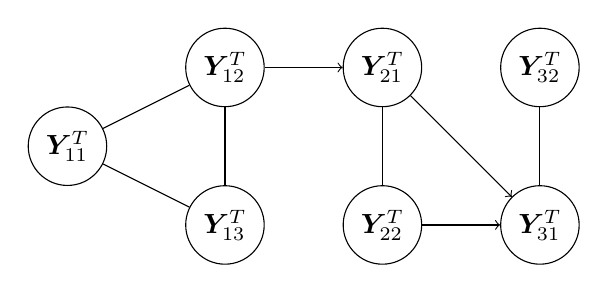
\begin{tikzpicture}[node distance= 2.5cm]
\node[draw,circle] (01) at (-1,-1) {$\bm{Y}_{11}^T$};
\node[draw,circle] (10) at (1,0) {$\bm{Y}_{12}^T$};
\node[draw,circle] (12) at (1,-2) {$\bm{Y}_{13}^T$};
\node[draw,circle] (20) at (3,0) {$\bm{Y}_{21}^T$};
\node[draw,circle] (22) at (3,-2) {$\bm{Y}_{22}^T$};
\node[draw,circle] (32) at (5,-2) {$\bm{Y}_{31}^T$};
\node[draw,circle] (30) at (5,0) {$\bm{Y}_{32}^T$};
\draw[-] (01) -- (10);
\draw[-] (01) -- (12);
\draw[-] (10) -- (12);
\draw[->] (10) -- (20);
\draw[-] (20) -- (22);
\draw[->] (20) -- (32);
\draw[->]  (22) -- (32);
\draw[-]  (32) -- (30);
\end{tikzpicture}}
\end{center}
\vspace{-.4cm}
\caption{Dynamic variant of the chain graph model in Figure \ref{fig:CG}. \label{fig:DCG}}
\end{figure}

\begin{example}
Consider the DCG defined by the CG of Figure \ref{fig:DCG}. Since the topology of this CG is the same as the one in Figure \ref{fig:CG}, this DCG has three strong components, corresponding, for each time slice $t\in[T]$, to $\bm{Y}_1(t)=(Y_{11}(t),Y_{12}(t),Y_{13}(t))^\T$, $\bm{Y}_{2}(t)=(Y_{21}(t),Y_{22}(t))^\T$ and $\bm{Y}_{3}(t)=(Y_{31}(t),Y_{32}(t))^\T$. Note that in this case we have $\bm{Y}(t)^\T=(\bm{Y}_1(t)^\T,\bm{Y}_2(t)^\T,\bm{Y}_3(t)^\T)$, as confirmed by Figure \ref{fig:CGDAG}. The observation equations are specified by the following vectors: $\bm{F}_1(t)^\T=(\bm{F}_{11}(t)^\T,\bm{F}_{12}(t)^\T,\bm{F}_{13}(t)^\T)$, functions of $\bm{y}^{t-1}_1$; $\bm{F}_2(t)^\T=(\bm{F}_{21}(t)^\T,\bm{F}_{22}(t)^\T)$, functions of $\bm{y}^{t-1}_2$, where $\bm{F}_{21}(t)$ is also a function of $\bm{y}^t_{13}$; $\bm{F}_3(t)^\T=(\bm{F}_{31}(t)^\T,\bm{F}_{32}(t)^\T)$, function of $\bm{y}^{t-1}_3$, where $\bm{F}_{31}(t)$ is also a function of $\bm{y}^t_2$. 
\end{example}

It can be shown that the results in Propositions \ref{prop:MDM} and \ref{prop:MDM2} for MDMs hold for DCGs if applied to the chain component observation series $\bm{Y}_i(t)$ and their associated system vectors $\bm{\theta}_i(t)$,  $i\in [N]$. Therefore in DCGs the sequential updating and forecasting of the  relevant probabilities can be distributed across the chain components of the underlying CG. 

\subsubsection{Dynamic Bayesian Networks.}
The two described multivariate models are not as commonly used in practice as the \textit{Dynamic Bayesian Network (DBN)} model class \citep{Murphy2002}. DBNs extend the BN framework to dynamic and stochastic domains. We discuss these models in this thesis to provide an example of a model class whose conditional independence structure is not retained as time progresses and therefore do not enjoy closed form updating routines.

 For the purpose of this thesis, and as often in practice, we consider only stationary, feed-forward DBNs respecting the first order Markov assumption \citep[see e.g.][]{Oates2013}. These DBNs can be simply described by an initial distribution over the first time point and a BN having as vertex set two generic time slices. Such latter BN is usually called 2-Time slice Bayesian Network (2-TBN).

\begin{definition}
\label{def:2-TBN}
A \emph{2-TBN} for $\{\bm{Y}(t)\}_{t\in[T]}$ is a BN with DAG $\Gr$ such that, fixed a  $t\in [T-1]$, $V(\Gr)=\{Y_i(t),Y_{i}(t+1):i\in[n]\}$, any vertex $Y_i(t)$ has no parents and there are no edges $(Y_{i}(r),Y_{j}(r))$, $i,j\in[n]$, $r=t,t+1$.   
\end{definition} 
    
\begin{figure}
\vspace{-.3cm}
\centerline{
\entrymodifiers={++[o][F-]}
\xymatrix{
Y_1(t)\ar[d]&Y_2(t)\ar[d]\ar[dl]&Y_3(t)\ar[d]\ar[dl]&Y_4(t)\ar[d]\ar[dl]\\
Y_{1}(t{+1})&Y_{2}(t{+1})&Y_{3}(t{+1})&Y_{4}(t{+1})
}
}
\caption{Example of a 2-time-slice Bayesian network for a multivariate time series comprising four univariate series. \label{fig:2-TBN}}
\end{figure}

\begin{definition}
A \emph{DBN} for the time series $\{\bm{Y}(t)\}_{t\in[T]}$ is a pair $(\Gr,\Gr')$, such that $\Gr$ is a BN with vertex set $V(\Gr)=\{Y_i(1):i\in[n]\}$, and $\Gr'$ is a 2-TBN such that its  vertex set $V(\Gr')$ is equal to $\{Y_i(t),Y_{i}(t+1):i\in[n]\}$.
\end{definition}

It is therefore straightforward to notice that a recursive formula for the density function of a DBN similar to the one for BNs in Lemma \ref{lemma:rec} exists. This is because a DBN can be thought of as the concatenation of BNs.

\begin{example}
\label{ex:DBN}
The BN in Figure \ref{fig:2-TBN} is a valid 2-TBN because its topology respects the conditions of Definition \ref{def:2-TBN}. Suppose a DBN has such 2-TBN and the BN associated to the initial distribution over $\bm{Y}(1)$ has empty edge set, i.e. represents the independence model in Definition \ref{def:indmodel}. Then its probability density function factorises as (suppressing the dependence on the parameter vector for ease of notation)
\begin{equation*}
\label{eq:exampleDBNfactorization}
f\left(\bm{y}^T\right)=\prod_{i\in[4]}f(y_i(1))\prod_{t\in[T]_1}f(y_4(t)\;|\;y_{4}(t{-1}))\prod_{j\in[3]}f(y_j(t)\;|\;y_{j}(t{-1}),y_{j+1}(t{-1}))
\end{equation*}
\end{example}

Although DBNs entail an effective recursive factorisation of the associated density function, thus requiring a low number of probabilities to be elicited in order to fully specify the model, inference in such models cannot be performed as easily as in both BNs and MDMs. This is because the initial conditional independence structure is broken through time. As shown in Figure \ref{fig:unrolled} \citep[from ][]{Boyen1998}, the so-called unrolled version of the DBN of Example \ref{ex:DBN}, after a small number of time steps all the variables in a same time slice become correlated with each other. Independence can only be retained if each component time series is independent of the others, i.e. if the 2-TBN has edges of the type $(Y_i(t),Y_i(t+1))$ and an initial distribution described by an independence model. Therefore the efficient and distributed recursions for both inference and forecasting associated to MDMs and DCGs do not transfer to generic DBNs. This is the reason why DBNs are not an effective model class for exact aggregation methods in the problems we address in Chapter \ref{chapter3}. However, we note here that a variety of methodologies based on stochastic approximated methods have been developed for tractable inferences in such models \citep{Boyen1998, Koller2001}. 

\begin{figure}
\vspace{-.3cm}
\centerline{
\scalebox{0.75}{
\entrymodifiers={++[o][F-]}
\xymatrix{
Y_1(1)\ar[r]&Y_1(2)\ar[r]&Y_1(3)\ar[r]&Y_1(4)\\
Y_2(1)\ar[r]\ar[ur]&Y_2(2)\ar[r]\ar[ur]&Y_2(3)\ar[r]\ar[ur]&Y_2(4)\\
Y_3(1)\ar[r]\ar[ur]&Y_3(2)\ar[r]\ar[ur]&Y_3(3)\ar[r]\ar[ur]&Y_3(4)\\
Y_4(1)\ar[r]\ar[ur]&Y_4(2)\ar[r]\ar[ur]&Y_4(3)\ar[r]\ar[ur]&Y_4(4)}}}
\caption{Unrolled version of the dynamic Bayesian network of Example \ref{ex:DBN} with 2-time-slice Bayesian network of Figure \ref{fig:2-TBN}.\label{fig:unrolled}}
\end{figure}

\subsection{Causality}
\label{sec:causality}
Statistical reasoning has historically largely avoided  investigating causal inferences. Classical methods, as for example regression analysis, are in general only able to predict new values of a variable given the values of a set of covariates, and how these relate to the response variable. Until recently, there has not been a formal study of causal relationships between sets of random variables to assess, for example, whether a variable can be considered as a \textit{cause} for another one or not. However, artificial intelligence researchers such as \citet{Pearl2000} and \citet{Spirtes1993}, provided a systematic study of the causal mechanisms underlying a given hypothesised BN model when certain variables are \textit{manipulated} and fixed to take a certain value in their sample space. This theory supposes the existence of an underlying idle system, i.e. one where its variables are observed and not manipulated to a certain value. 
 
We introduce here the concept of causality since, for the purpose of decision support, it is often helpful to match data coming from experiments in a laboratory, where variables are held fixed to a particular value, to observational one, to provide a revised and more focused specification of the relevant probabilities. 
 
\citet{Shafer1996} discusses causal reasoning for models depicted by trees. As also suggested by \citet{Smith2010}, trees are particularly suitable to represent causal relationships, since these can uniquely describe the actual narrative underlying the unfolding of events. We also note here that causal reasoning is more tenable for Bayesian decision analysis than in pure inferential reasoning since DMs need to think hard on how the problem at hand unfolds when eliciting both their probabilistic and preferential beliefs. Therefore, a DM's model can often be used to answer various causal questions \citep{Smith2010}.

We now formally define the concept of intervention as introduced in \citet{Pearl2000}.

 \begin{definition}
 A \emph{Perlean intervention} on $\bm{Y}_A$, $A\subset[n]$, consists of fixing these variables to a (known) value $\bm{y}_A$. The resulting density is written $f\left(\bm{y}\;|\;\do(\bm{Y}_A=\bm{y}_A)\right)$.
 \end{definition} 

As noted in Section \ref{sec:BN}, there are several BNs entertaining the same density factorisation and therefore leading to the same kind of inferences. Causal reasoning cannot thus be straightforwardly followed in generic BNs. We define here a particular class of BNs that are causal in the Perlean sense.

\begin{definition}
\label{def:cbn}
A BN $\Gr$ is a \emph{Causal Bayesian Network (CBN} if, for any Perlean intervention on $\bm{Y}_A$, $A\subset[n]$, it holds that 
\begin{equation*}
f\left(\bm{y}\;|\;\bm{\theta},\do(\bm{Y}_A=\bm{y}_A)\right)=\prod_{i\in[n]\setminus A}f\left(y_i\;|\;\bm{\theta}_i,\bm{y}_{\Pi_i}\right).
\end{equation*} 
\end{definition} 

\begin{example}
Consider the CBN with DAG in Figure \ref{fig:BNexample}. Suppose we intervene on this DAG and set $Y_2=y_2$. The resulting factorisation is equal to
\begin{equation*}
f\left(y_1,y_2,y_3,y_4\;|\;\bm{\theta},do(Y_2=y_2)\right)=f(y_1\;|\;\bm{\theta}_1)f(y_3\;|\;y_1,y_2,\bm{\theta}_3)f(y_4\;|\;y_1,\bm{\theta}_4).
\end{equation*}
Such intervention can be depicted graphically by deleting every edge into $Y_2$, in this case simply $(Y_1,Y_2)$, and changing the label of the vertex associated to the intervened variable to $Y_2=y_2$. Such DAG is reported in Figure \ref{figure:causalBN}.
\end{example}

\begin{figure}
\vspace{-.2cm}
\entrymodifiers={++[o][F-]}
\centerline{
\xymatrix{
\mbox{\large{$Y_4$}}&\mbox{\large{$Y_2=y_2$}}\ar[d]\\
\mbox{\large{$Y_1$}}\ar[u]\ar[r]&\mbox{\large{$Y_3$}}
}
}
\vspace{-.2cm}
\caption{
Causal version of the Bayesian Network in Figure \ref{fig:BNexample} under the intervention $Y_2=y_2$. \label{figure:causalBN}}
\end{figure}

\begin{definition}
For an intervention $\do(\bm{Y}_A=\bm{y}_A)$ over the variables of a CBN $\Gr$, $V(\Gr)=\{Y_i:i\in[n]\}$, we call \emph{manipulated DAG} $\Gr'$ the network with edge set $\E(\Gr')=\E(\Gr)\setminus\{(Y_i,Y_j)\in E(\Gr): j\in A\}$ and $V(\Gr')=\{Y_i: i\in \{[n]\setminus A\}\}\cup \{Y_i=y_i: i\in A\}$.
\end{definition}

If a BN is believed to be causal, then experimental evidence can be used to update the parameter densities as formalised below.

\begin{proposition}
 Suppose global independence holds and assume the experimental sample $\bm{x}$ from the same population as $\bm{Y}$ is ancestral with respect to the manipulated DAG for the intervention $do(\bm{Y}_A=\bm{y}_A)$. Let $I$ be the set of indices of both the vertices whose children are not sampled and the leaves of the DAG. Then, for a CBN the posterior factorises as
 \begin{equation*}
 \pi(\bm{\theta}\;|\;\bm{x})=\prod_{i\in I}\prod_{\substack{j\in A_i\\j\not\in A}}\pi(\bm{\theta}_j\;|\;\bm{x})\prod_{k\not\in \{A_i\cup A\}}\pi(\bm{\theta}_k).
 \end{equation*}
\end{proposition}

The concept of causality for BNs has been extended in \citet{Daneshkhah2004} to take into account manipulations of the parameter vector, usually called \textit{randomised interventitions} \citep[see e.g.][]{Lauritzen2001, Daneshkhah2004}.  These consist of fixing a random parameter of the density of a random variable to take a particular known value.   \citet{Daneshkhah2004} defined the concept of an hypercausal BN, which is one where certain randomised interventions respect the topology of the DAG. Most importantly they showed that local and global independence holds iff the BN is hypercausal and therefore also in the case the model is a CBN. Thus the validity of the causal assumption can be checked through reasoning about the faithfulness of global and local independence and vice versa. In Chapter \ref{chapter3} below we define a new class of randomised interventions related to committing to a countermeasure policy. We are able to show that Perlean interventions in CBNs can be seen as a special case of our methodology.  
 
We have focused here on causality over graphical directed structures, since these naturally provide a framework for causal reasoning. In these models variables are ordered and there are no symmetric relationships. This is the reason why causal arguments in MN models are much more difficult to develop \citep[see e.g.][]{Lauritzen2002}. Although much of the literature on statistical causality centred on the BN model class, the causal semantic has been extended to a variety of frameworks, e.g. CEGs \citep{Thwaites2010,Thwaites2013}, CGs \citep{Lauritzen2002}, DBNs \citep{Eichler2007}, IDs \citep{Dawid2002a}, MDMs \citep{Queen2009} and  others \citep{Aalen2012, Dawid2010, Smith2007}.  We point out that \citet{Dawid2010} developed causal arguments in the framework of \textit{dynamic treatment strategies} \citep{Murphy2003}. These are dynamic models in medical contexts where the objective is to identify the causal effect of a particular treatment. The computation of these effects is based on backward inductive arguments, which mirror the recursions we develop in Chapter \ref{chapter4} for IDSSs. 
 
\subsection{Emulators} 
\label{sec:emu}
Although probabilistic reasoning is now widespread in many areas of science, deterministic modelling is still often performed in practice as noted in Chapter \ref{chapter1}. Such deterministic models usually consist of huge simulators using approximate methods to numerically solve big systems of differential equations describing some natural process. This is often the case in climate change modelling for example \citep{Rougier2015}.

Even if we believed these simulator models were true - which would be heroic - for coherent Bayesian analyses to use these, there is the need to define a probability distribution over the corresponding space of possibilities. This is because unmodelled uncertainty appears at various stages of the deterministic computations of simulators, as extensively discussed in \cite{Kennedy2000}. Probability distributions are then usually achieved by building an \textbf{emulator} over their outputs. The literature on emulators is now very vast \citep{Kennedy2006, Kennedy2001,OHagan2006,Santner2003} and for the purpose of this thesis we focus here only on Bayesian methods. Within the Bayesian literature a variety of methodologies have been developed to account for both large-dimensional and dynamic outputs \citep{Conti2009,Liu2009, Rougier2008,Craig2001, Goldstein2006, Williamson2011}.

\subsubsection{Modelling of Computer Outputs.}
A simulator is a function $g(\cdot)$ that maps inputs $\bm{z}\in\bm{\mathcal{Z}}$, for some arbitrary space $\bm{\mathcal{Z}}$, into an output $y=g(\bm{z})$. In its vanilla form the output $y$ is univariate and constant through time. Often in practice only a small set of training runs at inputs $\bm{z}_1,\dots, \bm{z}_N$ of the simulator are available, whose outputs $y_1=g(\bm{z}_1),\dots, y_N=g(\bm{z}_N)$ are observed and treated as data. Only a small number of such outputs can be observed since simulators are usually slow and each single evaluation can take weeks if not months. An emulator is then an approximation $\hat{g}(\cdot)$ of $g(\cdot)$ such than at an input point $\bm{z}_i$, $\hat{g}(\bm{z}_i)=g(\bm{z}_i)$, whilst at other points it consists of a distribution whose mean represents a plausible interpolation of the training runs and its variance the uncertainty associated to such interpolation.

\subsubsection{Gaussian Process Modelling.}
The most common modelling technique is to assume that $g(\cdot)$ behaves as a \textit{Gaussian Process (GP)}. Formally, $g(\cdot)$ has a GP distribution if, for every $N\in\mathbb{Z}_{\geq 1}$, the joint distribution of $g(\bm{z}_1),\dots,g(\bm{z}_N)$ is multivariate Normal for all $\bm{z}_1,\dots,\bm{z}_N\in\bm{\mathcal{Z}}$. The distribution of the GP is therefore characterised by its mean $m(\bm{z})=\mathbb{E}(g(\bm{z}))$ and its covariance function $c(\bm{z},\bm{z}')=\Cov(g(\bm{z}),g(\bm{z}'))$, for $\bm{z},\bm{z}'\in\bm{\mathcal{Z}}$. In general, $m(\cdot)$ may be any function, but $c(\cdot,\cdot)$ is non negative definite for every $\bm{z}_1,\dots,\bm{z}_N\in\bm{\mathcal{Z}}$ and any $N\in\mathbb{Z}_{\geq 1}$. The mean and covariance functions are usually modelled hierarchically as $
g(\bm{z})=m(\bm{z})+e(\bm{z})=\bm{h}(\bm{z})^\T\bm{\beta}+e(\bm{z}),$
where $\bm{h}(\bm{z})=(h_i(\bm{z}))_{i\in[p]}^\T$ is a vector of $p$ known functions, $\bm{\beta}=(\beta_i)_{i\in[p]}^\T$ is a vector of $p$ unknown coefficients and $e(\bm{z})$ is a mean-zero GP  with covariance $c(\cdot,\cdot)$. The vector $\bm{h}$ often simply consists of simple monomial functions of $\bm{z}$. The covariance is usually defined as $c(\bm{z},\bm{z}')=\psi r(\bm{z}-\bm{z}')$, where $r(\cdot)$ is a correlation function such that $r(0)=1$, $\bm{z},\bm{z}'\in\bm{\mathcal{Z}}$, and $\psi\in\mathbb{R}_{>0}$. This choice implies a stationary process since the correlation only depends on the distance between two points. A variety of correlation functions have been defined in the literature and these are often used in geostatistical modelling \citep[see e.g.][]{Diggle2007}. The model definition is then completed by eliciting a prior distribution over the parameters $\bm{\beta}$ and $\psi$. Often a weak improper prior is given to such parameters, but conjugate analysis can be performed by choosing appropriate prior distributions just as in the Normal linear model case \citep[see e.g.][]{Haylock1996}. 

Once an emulator is built, using for example the GP structure we exemplified here, each evaluation of the simulator can be used to update the  probability distribution of the emulator in a Bayesian fashion. Furthermore, additional uncertainty measures can be included in the modelling. For example, calling $y_i'$ the true value of the system the simulator is modelling, given observed inputs $\bm{z}_i$, one could set $y_i'=g(\bm{z}_i)+v$, where $v$ is some error following for example a Gaussian distribution \citep[see][for more comments on these modelling techniques]{Kennedy2000}.

\section{Utility Models}
\label{sec:ut}
The other main ingredient of the SEU model is the utility function $u(\bm{r},d)$. In this section we provide a broad overview of utility theory with a particular focus to the multiattribute case, i.e. when $\bm{R}$ is large dimensional. Let $\bm{R}=(R_i)_{i\in[m]}^\T$ and $\bm{r}$ and $r_i$ be instantiations of $\bm{R}$ and $R_i$  taking values in $\bm{\mathcal{R}}$ and $\mathcal{R}_i$ respectively. Note that in the notation of Section \ref{sec:SEU}, each $R_i$ can correspond to random quantities, decisions, or a combination of the two. 

 Here we first introduce independence concepts for preferences mirroring those for probabilistic reasoning. We  then show how particular sets of independence assumptions can lead to classes of utility factorisations that, just as in the probabilistic case, can highly reduce the burden of utility elicitation. We then consider fairly recent utility factorisations that arise from underlying graphical models depicting preferential indifferences. We conclude the section with a review of utility theory for single attributes which, under the assumption of a particular utility factorisation, comes often into play in multivariate settings. 

Before that, we  briefly summarise important aspects of utility theory that we do not deal with in this thesis since these are not central for our results. Firstly, we do not discuss value functions, although these are widely used in practice \citep{Belton2002,Keeney1993a}. There are two main reasons for this: one, the coherence and the rationale of the Bayesian formalism is retained only using utility functions; two, value functions, differently from utilities, are not able to represent attitudes towards risk. 

Secondly, we  assume in this thesis that the vector $\bm{R}$ includes a \textit{complete} and \textit{non-redundant} collection of attributes so that this covers all the important aspects of the problem and each factor is not double counted. In addition each $R_i$ has to be \textit{operational} so that it can be meaningfully used in the analysis and the DM can provide true preferential assessments about it.  More broadly, we assume that the vector $\bm{R}$ includes all the relevant factors of the system under study and the DM can uniquely provide preferential assessments over its elements. In practice to identify such a vector of attributes an \textit{objective tree} \citep{Keeney1993a} is built, which breaks down each attribute into sub-attributes until the leaves of the tree consist of operational attributes only. An example of the objective tree elicited during the Chernobyl project is presented in Figure \ref{fig:objtree}. The root of this tree is the main factor related to a nuclear emergency: how the accident affects humans' living condition. This is then split in two sub-attributes: one concerning the effects of the accident, the second the use of resources. Effects is again split in two sub-attributes and the process continues in this fashion until a vertex represents an operational attribute. Each leaf of this tree would then correspond in our notation to an element $R_i$ of $\bm{R}$.

Finally, we do not discuss techniques to assess and elicit utility functions, either their algebraic form or their  features \citep[see e.g.][]{Clemen1996a,Keeney1993a,  Keeney2009,von1986}. These are however fundamental in any formal decision analysis to faithfully represent the preferences of DMs.

\begin{figure}
\vspace{-.3cm}
\begin{center}
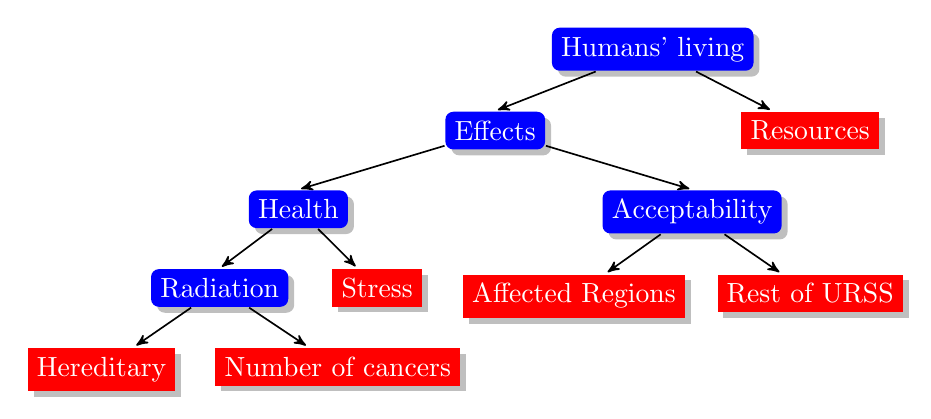
\begin{tikzpicture}[>=stealth',shorten >=1pt,auto,semithick,
    fact/.style={rectangle, draw=none, rounded corners=1mm, fill=blue, drop shadow,
        text centered, anchor=north, text=white},
        leaf/.style={rectangle, draw=none, fill=red,
        text centered, anchor=north, text=white, drop shadow},
    level distance=0.5cm, growth parent anchor=south
]
\tikzstyle{every state}=[every text node part/.style={align=center}]
\node (State00) [fact] {Humans' living} [->] [sibling distance=4cm]
child{  [sibling distance=5cm]
        node (Fact01) [fact] {Effects}
        child{ [sibling distance=2cm]
        node (Fact11) [fact] {Health}
        child{[sibling distance=3cm]
        node (Fact21) [fact] {Radiation}
        child{ 
        node (Fact31) [leaf] {Hereditary}
        }
        child{
        node (Fact31) [leaf] {Number of  cancers}
        }
        }
        child{
        node (Fact23) [leaf] {Stress}
        }
        }
        child{
        [sibling distance=3cm]
        node (Fact33) [fact] {Acceptability}
        child{
        node (leaf11) [leaf] {Affected  Regions}
        }
        child{
        node (leaf22) [leaf] {Rest of  URSS}
        }
        }
        }
child{
        node (Fact02) [leaf] {Resources}
        }
        ;
\end{tikzpicture}
\end{center}
\vspace{-.4cm}
\caption{Objective tree elicited at the end of the Chernobyl project from \citet{Papamichail2013}. The vertices in red of the tree are leaves, whilst the blue ones are positions. \label{fig:objtree}}
\end{figure}
 
\subsection{Independence Concepts}
As the dimension of $\bm{R}$ might be arbitrarily large, a variety of independence concepts have been introduced in the literature to both simplify the utility elicitation and describe various sets of indifferences. We introduce a few of these following \citet{Keeney1993a}.

\begin{definition}
\label{def:utind}
An attribute $\bm{R}_A$ is said to be \textbf{Utility Independent (UI)} of $\bm{R}_B$, for a partition $A$, $B$ of $[m]$,\footnote{More generally, a partition $B_1,\dots,B_n$ of a set $[m]$ is such that $\cup_{i\in[n]}B_i=[m]$ and $\cap_{i\in[n]}B_i=\emptyset$.} if the utility for $\bm{R}_A$ does not change when the attributes in $\bm{R}_B$ are varied.
\end{definition}

\begin{proposition}
Under the conditions of Definition \ref{def:utind}, if $\bm{R}_A$ is UI of $\bm{R}_B$ then $ u(\bm{r})=a(\bm{r}_B)+b(\bm{r}_B)u(\bm{r}_A)$, where $a(\cdot)$ and $b(\cdot)>0$ depend on $\bm{r}_{B}$ and not on $\bm{r}_A$. 
\end{proposition}

In order to understand the meaning of this independence, consider the following example. If the DM believes that the prevalence of tumours is UI of the amount of contamination, then the utility function describing the prevalence of tumours does not depend on the level of contamination of the area. For example, the utility of having a low number of cancer cases would be the same both when the area is highly contaminated and when there is no radiation at all. Note that utility independence is not necessarily symmetric: if the prevalence of tumours is UI of the level of contamination then it does not follow that the converse is true.

We now consider two particular sets of utility independence statements.

\begin{definition}
We say that $\bm{R}$ has \emph{singly UI attributes} if  $R_i$ UI $\bm{R}_{[m]\setminus \{i\}}$, for every $i\in[m]$.
\end{definition}

\begin{definition}
We say that $\bm{R}$ has \emph{mutually UI attributes} if, for every $A\subseteq[m]$, $\bm{R}_A$ UI $\bm{R}_{[m]\setminus A}$.
\end{definition}

We now consider a generalisation of utility independence \citep[see e.g.][]{Abbas2010}.
\begin{definition}
\label{def:cutind}
An attribute $\bm{R}_A$ is said to be \textbf{Conditional Utility Independent (CUI)} of $\bm{R}_B$ given $\bm{R}_C$, for a partition $A$, $B$, $C$ of $[m]$, if the utility of $\bm{R}_A$ does not change when the attributes in $\bm{R}_B$ are varied, for each instantiation of $\bm{R}_C$.
\end{definition}


\begin{proposition}
Under the conditions of Definition \ref{def:cutind}, if $\bm{R}_A$ is CUI of $\bm{R}_B$ given $\bm{R}_C$ then
\begin{equation}
u(\bm{r})=a(\bm{r}_B,\bm{r}_C)+b(\bm{r}_B,\bm{r}_C)h(\bm{r}_A,\bm{r}_C)
\label{eq:cui}
\end{equation}
for some $a$, $h$ and $b>0$, functions of their arguments only. 
\end{proposition}

In order to give an explicit form to the function $h$ of equation (\ref{eq:cui}) in terms of utilities, we introduce a generalisation of the utility function of Definition \ref{def:ut}, which more easily can represent CUI statements. Let $\bm{r}_A^{*}=(r_i^{*})^\T_{i\in A}$ and $\bm{r}_A^0=(r_i^0)^\T_{i\in A}$, $A\subseteq [n]$, where $r_i^*$ and $r_i^0$ are respectively the best and the worst outcome of attribute $R_i$. 

\begin{definition}
\label{def:cui}
The \emph{normalised conditional utility} function for $\bm{R}_A$ given $\bm{R}_{[m]\setminus A}$ is defined as
\begin{equation*}
u(\bm{r}_A\;|\; \bm{r}_{{[m]\setminus A}})=\frac{u(\bm{r}_A,\bm{r}_{[m]\setminus A})-u(\bm{r}_A^0,\bm{r}_{[m]\setminus A})}{u(\bm{r}_A^*,\bm{r}_{[m]\setminus A})-u(\bm{r}_A^0,\bm{r}_{[m]\setminus A})}.
\end{equation*}
We also define the \emph{normalised conditional disutility} function as
\begin{equation*}
\check{u}(\bm{r}_A\;|\;\bm{r}_{[m]\setminus A})=1-u(\bm{r}_A\;|\;\bm{r}_{[m]\setminus A})
\end{equation*}
\end{definition}

From e.g. \citet{Abbas2010} we have the following.
\begin{proposition}
Under the conditions of Definition \ref{def:cutind}, if $\bm{R}_A$ CUI $\bm{R}_B$ given $\bm{R}_C$ then
\begin{equation*}
u(\bm{r}_A\;|\; \bm{r}_B,\bm{r}_C)=u(\bm{r}_A\;|\; \bm{r}_B^0,\bm{r}_C)=u(\bm{r}_A\;|\; \bm{r}_B^{*},\bm{r}_C).
\end{equation*}
Furthermore, the terms in equation (\ref{eq:cui}) can be written as 
$
a(\bm{r}_B,\bm{r}_C)=u(\bm{r}_A^0,\bm{r}_B,\bm{r}_C)$, $b(\bm{r}_B,\bm{r}_C)=u(\bm{r}_A^*,\bm{r}_B,\bm{r}_C)-u(\bm{r}_A^0,\bm{r}_B,\bm{r}_C)$ and $h(\bm{r}_B,\bm{r}_C)=u(\bm{r}_C\;|\;\bm{r}_B^0,\bm{r}_C)$.
\end{proposition}

We now introduce a different class of independence concepts. 

\begin{definition}
Let $B_1,\dots,B_k$ be a partition of $[m]$. Attributes $\bm{R}_{B_1},\dots, \bm{R}_{B_k}$ are said  to be \emph{additive independent} if the preference comparison of any two lotteries, defined as probability distributions over $\bigtimes_{i\in[k]} \bm{\mathcal{R}}_{B_i}$, depends only on their marginal probability distributions.
\end{definition}

Additive independence can be generalised to the case where the indices of the attributes do not form a partition of $[m]$. 
\begin{definition}
\label{def:GAI}
Let $B_1,\dots,B_k$ be such that $\cup_{i\in[k]}B_i=[m]$. Attributes $\bm{R}_{B_1},\dots, \bm{R}_{B_k}$ are said to be \textbf{Generalized Additive Independent (GAI)} if  the preference comparison of any two lotteries depends only on the marginal probability distributions over $\bigtimes_{i\in[k]} \bm{\mathcal{R}}_{B_i}$.
\end{definition}

\subsection{Utility Factorisations}
The sets of independences introduced in the previous section give rise to specific factorisations of the overall utility function. Suppose each function $u_A(\bm{r}_A)$, a marginal utility function over $\bm{R}_A$ only, is such that $u_i(\bm{r}_A^0)=0$ and $u_i(\bm{r}_A^*)=1$, $A\subseteq [m]$. The following results, from e.g. \citet{Keeney1993a}, hold.

\begin{proposition}
If a utility function $u(\bm{r})$ has $m$ singly UI attributes, then it must take the form 
\begin{equation}
\label{eq:multilinear}
u(\bm{r})=\sum_{A\in\mathcal{P}_0([m])}k_A\prod_{i\in A} u_i(r_i),
\end{equation}
where $\mathcal{P}_0$ denotes the power set without the empty set and $k_A\in [0,1]$ is a \textit{criterion weight} \citep{Keeney1993a} such that $\sum_{A\subseteq[m]}k_A=1$.
\end{proposition} 

\begin{definition}
\label{def:multilinear}
Utility functions entertaining the factorisation in equation (\ref{eq:multilinear}) are called \textbf{multilinear}.
\end{definition}

The criterion weights of equation (\ref{eq:multilinear}) can be evaluated by comparing the utility of terms $u(\bm{r}_A^*,\bm{r}_{[m]\setminus A}^0)$. Their actual form is not fundamental for this thesis and can be found in \citet{Keeney1993a}. 

\begin{proposition}
\label{prop:multiplicative}
If a utility function $u(\bm{r})$ has $m$ mutually UI attributes, then it must take the form
\begin{equation}
\label{eq:multiplicative}
u(\bm{r})=\sum_{A\in\mathcal{P}_0([m])}h^{n_A-1}\prod_{i\in A}k_iu_i(r_i),
\end{equation}
where $n_A$ is the number of elements in $A$, $k_i=u(r_i^*,\bm{r}_{[n]\setminus \{i\}}^0)$ and $h$ is the unique solution not smaller than minus one to
\begin{equation}
\label{eq:h}
1+h=\prod_{i\in[m]}(1+hk_i).
\end{equation}
\end{proposition}

\begin{definition}
\label{def:multiplicative}
Utility functions entertaining the factorisation in equations (\ref{eq:multiplicative}) and (\ref{eq:h}) are called \textbf{multiplicative}.
\end{definition}

\begin{example}
Consider three attributes $R_1$, $R_2$ and $R_3$. A multilinear factorisation over these attributes can be written as
\begin{equation*}
u=k_1u_1+k_2u_2+k_3u_3+k_{12}u_1u_2+k_{13}u_1u_3+k_{23}u_{2}u_3+k_{123}u_1u_2u_3,
\end{equation*}
whilst the multiplicative one has the form
\begin{equation}
\label{eq:examplemultilinear}
u=k_1u_1+k_2u_2+k_3u_3+hk_{1}k_{2}u_1u_2+hk_{1}k_{3}u_1u_3+hk_{2}k_{3}u_{2}u_3+h^2k_{1}h_{2}k_{3}u_1u_2u_3,
\end{equation}
where for ease of notation we left the arguments of these functions implicit.
\end{example}
We can note that the multiplicative factorisation is a special case of the multilinear one.  Importantly, in the multilinear case there are $2^m-2$ criterion weights to elicit, whilst in the multiplicative one these are only $m$. Therefore the elicitation task is much simpler in the multiplicative case. 

\begin{proposition}
If a utility function $u(\bm{r})$ has $m$ additive independent attributes then it must take the form
\begin{equation}
\label{eq:additive}
u(\bm{r})=\sum_{i\in[m]}k_iu_i(r_i),
\end{equation}
where $\sum_{i\in [m]}k_i=1$.
\end{proposition}

\begin{definition}
Utility functions entertaining the factorisation in equation (\ref{eq:additive}) are called \textbf{additive}.
\end{definition}

Additive utility functions can be considered as special cases of multiplicative utility functions, and therefore also of multilinear ones, by noting equation (\ref{eq:additive}) coincides with equation (\ref{eq:multiplicative}) in the case the weights of Proposition \ref{prop:multiplicative} sum to unity.

\begin{example}
An additive factorisation over three attributes $R_1$, $R_2$ and $R_3$ can be written as
\begin{equation*}
\label{eq:exampleadditive}
u(r_1,r_2,r_3)=k_1u_1(r_1)+k_2u_2(r_2)+k_3u_3(r_3)
\end{equation*}
\end{example}

\begin{proposition}
\label{prop:gai}
Suppose $\bm{R}_{B_1},\dots,\bm{R}_{B_k}$ are GAI, where $B_1,\dots, B_k$ are such that $\cup_{i\in[k]}B_i=[m]$, then
\begin{equation}
\label{eq:GAI}
u(\bm{r})=\sum_{i\in[k]}u_i(\bm{r}_{B_i}).
\end{equation}
\end{proposition}

\begin{example}
Consider again three attributes $R_1$, $R_2$ and $R_3$ and assume $\{R_1,R_2\}$ and $\{R_2,R_3\}$ are GAI. Then
\begin{equation}
\label{eq:GAIexample}
u(r_1,r_2,r_3)=u_{12}(r_1,r_2)+u_{23}(r_2,r_3).
\end{equation} 
Note however that the functions  $u_{12}$ and $u_{23}$ are not uniquely defined. \citet{Braziunas2005} and \citet{fishburn} showed that in this example the utility function in general decomposes as
\begin{equation}
\label{eq:GAIexample2}
u(r_1,r_2,r_3)=u(r_1,r_2,r_3^0)+u(r_1^0,r_2,r_3)+u(r_1^0,r_2,r_3^0).
\end{equation}
Therefore the third term on the right hand side (rhs) of equation (\ref{eq:GAIexample2}) can be associated to either of the first two terms of the rhs of equation (\ref{eq:GAIexample}). \citet{fishburn} defined the so called canonical decomposition which uniquely identifies the subutility functions.
\end{example}

\subsection{Graphical Utility Models}
The most general case of the previous section still assumes that all the attributes are utility independent of their complement. We note here that there are situations where this assumption is not tenable and at least one attribute is not utility independent of its complement. Such a situation is usually referred to as \textit{partial utility independence}. \citet{Abbas2010} derived a general expansion theorem for multiattribute utility functions which decomposes the overall function into a linear combination of products of conditional utility functions of Definition \ref{def:cui}. The resulting expression can then be simplified using CUI statements similarly to conditional independence in probabilistic reasoning. The underlying CUI structure can be represented by a network, exhibiting the same expressive power of network representations of probabilistic conditional independences. 

For the purpose of this thesis we mostly focus on the work of \citet{Abbas2010}, but we note here that other authors have proposed solutions to factorise multiattribute utility functions in the partial utility independence case. \citet{Farquhar1975} presented a decomposition theorem for utility independence structures called fractional hypercubes; \citet{Abbas2005} introduced a class of utility functions called attribute dominance utility, where utility is equal to zero whenever any attribute is at its worst outcome, and deduced expansion theorems for such a class; \citet{Bell1979} introduced multiattribute factorisations using interpolation techniques. 

We also note  that a variety of graphical representations of different sets of preferential independences have been defined. Again in this thesis we  mostly focus on \citet{Abbas2010} which introduced \textit{bidirectional utility diagrams} to represent sets of CUI statements. These diagrams are a generalisation of the utility diagrams of \citet{Abbas2005}, which only describe attribute dominance utilities. In the following chapters we  restrict our attention to a particular subclass of bidirectional utility diagrams, that can also be thought of as CUI networks \citep{Engel2008}. Graphical models based on additive independences also exist \citep{Bacchus1995, Braziunas2005}. Lastly, we note that \citet{Mura99} introduced expected utility networks that simultaneously represent probabilistic and preferential independences. 


We first present the expansion theorem of \citet{Abbas2010}. Let $\bm{\mathcal{R}}_A^{0*}$ be the set of all possible instantiations of $\bm{R}_A$ such that, for $i\in A$, $R_i$ is either at its maximum or at its minimum value, $A\subset [m]$. Suppose $A$ is totally ordered and, for $i\in A$, let $B_i$ be the subset of $A$ including the successors of $i$ in $A$ according to this order. Further let $V_i=A\setminus \{B_i\cup \{i\}\}$.

\begin{proposition}
\label{prop:utexpansion}
For any $A\subseteq[m]$, $u(\bm{r})$ can be written as
\begin{equation}
\label{eq:genut}
u(\bm{r})=\sum_{\bm{r}_A^{0*}\in \bm{\mathcal{R}}_A^{0*}}u(\bm{r}_A^{0*},\bm{r}_{[m]\setminus A})\prod_{i\in A}g(r_i\;|\; \bm{r}_{B_i}^{0*},\bm{r}_{V_i}),
\end{equation}
where 
\begin{equation*}
g(r_i\;|\; \bm{r}_{B_i}^{0*},\bm{r}_{V_i})=\left\{
\begin{array}{ll}
u(r_i\;|\; \bm{r}_{B_i}^{0*},\bm{r}_{V_i}),& \mbox{if } r_i=r_i^* \mbox{ in } u(\bm{r}_A^{0*},\bm{r}_{[m]\setminus A}) ,\\
\check{u}(r_i\;|\; \bm{r}_{B_i}^{0*},\bm{r}_{V_i}),&\mbox{if } r_i=r_i^0 \mbox{ in } u(\bm{r}_A^{0*},\bm{r}_{[m]\setminus A}).
\end{array}
\right.
\end{equation*}
\end{proposition}


\begin{example}
\label{ex:genut}
Consider three attributes $R_1$, $R_2$ and $R_3$. A generic decomposition for $u(r_1,r_2,r_3)$ assuming $3\succ 2\succ 1$, where $\succ$ is the order relation, can be written as
\begin{eqnarray}
u(r_1,r_2,r_3)&=&u(r_1^*,r_2^*,r_3^*)u(r_3\;|\;r_2,r_1)u(r_2\;|\; r_3^*,r_1)u(r_1\;|\; r_3^*,r_2^*)+\nonumber\\
&&u(r_1^0,r_2^*,r_3^*)u(r_3\;|\;r_2,r_1)u(r_2\;|\; r_3^*,r_1)\check{u}(r_1\;|\; r_3^*,r_2^*)+\nonumber\\
&&u(r_1^*,r_2^0,r_3^*)u(r_3\;|\;r_2,r_1)\check{u}(r_2\;|\; r_3^*,r_1)u(r_1\;|\; r_3^*,r_2^0)+\nonumber\\
&&u(r_1^*,r_2^*,r_3^0)\check{u}(r_3\;|\;r_2,r_1)u(r_2\;|\; r_3^0,r_1)u(r_1\;|\; r_3^0,r_2^*)+\nonumber\\
&&u(r_1^0,r_2^0,r_3^*)u(r_3\;|\;r_2,r_1)\check{u}(r_2\;|\; r_3^*,r_1)\check{u}(r_1\;|\; r_3^*,r_2^0)+\nonumber\\
&&u(r_1^0,r_2^*,r_3^0)\check{u}(r_3\;|\;r_2,r_1)u(r_2\;|\; r_3^0,r_1)\check{u}(r_1\;|\; r_3^0,r_2^*)+\nonumber\\
&&u(r_1^*,r_2^0,r_3^0)\check{u}(r_3\;|\;r_2,r_1)\check{u}(r_2\;|\; r_3^0,r_1)u(r_1\;|\; r_3^0,r_2^0).\label{eq:puiexample1}
\end{eqnarray}
The first term in each monomial can be written as a linear combination of criterion weights, whilst all the other conditional utilities have a single argument.
\end{example}

The utility decomposition in equation (\ref{eq:genut}) can be simplified using various sets of CUIs. These can be represented by the so called bidirectional utility diagrams. Here we slightly change the definition of \citet{Abbas2010} and represent these as CGs.

\begin{definition}
A \emph{bidirectional utility diagram} is a chain graph $\Gr$ with vertex set $\{R_1,\dots,R_m\}$ and whose edges represent the possibility of utility dependence as follows:
\begin{itemize}
\item if $(R_i,R_j),(R_j,R_i)\not\in E(\Gr)$, then $R_i$ is CUI of $R_j$ given $\bm{R}_{[m]\setminus \{i,j\}}$ and  $R_j$ is CUI of $R_i$ given  $\bm{R}_{[m]\setminus \{i,j\}}$;
\item if $(R_i,R_j)\in E(\Gr)$ but $(R_j,R_i)\not\in E(\Gr)$ then  $R_i$ is CUI of $R_j$ given $\bm{R}_{[m]\setminus \{i,j\}}$;
\item if $(R_i,R_j),(R_j,R_i)\in E(\Gr)$ then no utility independence is implied.
\end{itemize}
\end{definition}



\begin{example}
In Figure \ref{fig:biut} we present an example of a bidirectional diagram. This diagram includes only a directed edge and therefore represents the closest situation to a multilinear factorisation, corresponding to a diagram with no edges. This diagram asserts that $R_1$ is UI of $\{R_2,R_3\}$ and vice versa, plus that $R_3$ is CUI of $R_2$ given $R_1$. Therefore, using the CUI statements associated to the diagram in Figure \ref{fig:biut}, equation (\ref{eq:puiexample1}) can be rewritten as
\begin{eqnarray*}
u&=&u(r_1^*,r_2^*,r_3^*)u(r_3\;|\;r_2^*)u(r_2\;|\; r_3^*)u(r_1)+
u(r_1^0,r_2^*,r_3^*)u(r_3\;|\;r_2^*)u(r_2\;|\; r_3^*)\check{u}(r_1)+\nonumber\\
&&u(r_1^*,r_2^0,r_3^*)u(r_3\;|\;r_2^0)\check{u}(r_2\;|\; r_3^*)u(r_1)+
u(r_1^*,r_2^*,r_3^0)\check{u}(r_3\;|\;r_2^0)u(r_2\;|\; r_3^0)u(r_1)+\nonumber\\
&&u(r_1^0,r_2^0,r_3^*)u(r_3\;|\;r_2^0)\check{u}(r_2\;|\; r_3^*)\check{u}(r_1)+
u(r_1^0,r_2^*,r_3^0)\check{u}(r_3\;|\;r_2^*)u(r_2\;|\; r_3^0)\check{u}(r_1)+\nonumber\\
&&u(r_1^*,r_2^0,r_3^0)\check{u}(r_3\;|\;r_2^0)\check{u}(r_2\;|\; r_3^0)u(r_1).\label{eq:puiexample2}
\end{eqnarray*}
\end{example}


\begin{figure} 
\vspace{-.2cm}
\begin{center}
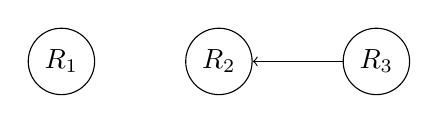
\begin{tikzpicture}[node distance=3cm]
\node[draw,circle] (11) at (-2,0) {$R_1$};
\node[draw,circle] (02) at (0,0) {$R_2$};
\node[draw,circle] (22) at (2,0) {$R_3$};
\draw[->] (22) -- (02);
\end{tikzpicture}
\end{center}
\vspace{-.4cm}
\caption{Example of a bidirectional utility diagram over three attributes. \label{fig:biut}}
\end{figure}

\citet{Abbas2010} identifies classes of bidirectional utility diagrams which give rise to optimal expansions of the multiattribute utility function, i.e. those where the conditional utility functions include the lowest number of arguments. 

For the purpose of this thesis we consider only a subclass of bidirectional utility diagrams. This was defined in \citet{Leonelli2015}.
 
\begin{definition}
\label{def:dirutdia}
We say that a bidirectional utility diagram is a \emph{directional utility diagram} if its graph is a DAG.
\end{definition}
Note that the diagram in Figure \ref{fig:biut} is unconventional in the sense that an attribute is parent of another one having a lower index. We  motivate this choice in Chapter \ref{chapter4}, where such diagrams proves to be very useful. Directional utility diagrams are extremely powerful in the multi-expert domains we address in later chapters, since the utility function associated to such diagrams can be written in terms of criterion weights and univariate utility functions. This is formalised in the following lemma.
\begin{lemma}
\label{lemma:ut}
For a directional utility diagram with vertex set $\{R_i:i\in[m]\}$ there exists an expansion order such that equation  (\ref{eq:genut}) is a linear combination of terms involving only criterion weights and conditional utility/disutility function having as argument a single attribute. 
\end{lemma}
\begin{proof}
This result follows by observing that the terms $u(\bm{r}_A^{0*},\bm{r}_{[m]\setminus A})$ in equation (\ref{eq:genut}) coincide with $u(\bm{r}_{[m]}^{0*})$ since the expansion can be performed over all the attributes. These terms are functions of criterion weights. Furthermore the conditional independence structure underlying a directed utility diagram is such that there is an expansion order where $R_i$ UI $\bm{R}_{V_i}\;|\; \bm{R}_{[m]\setminus \{V_i\cup i\}}$. Thus $g(r_i\;|\; \bm{r}_{B_i}^{0*},\bm{r}_{V_i})$ in equation (\ref{eq:genut}) is equal to $g(r_i\;|\; \bm{r}_{B_i}^{0*})$.
\end{proof}

\subsection{Univariate Utility Theory}
\label{sec:univariate}
In the previous sections we have shown how multiattribute utility problems can be decomposed into univariate ones when various sets of independences are believed to hold. We now discuss some of the characteristics of univariate utility functions and provide various examples. 

First, recall that utility functions are unique up to affine transformations, meaning that they imply the same preference ranking. Two such functions are said to be \textit{strategically equivalent}. In addition, \citet{Keeney1993a} showed that if two utility functions are strategically equivalent, then one must be an affine transformation of the other. 

We now introduce a variety of utility functions widely used in practice. 
\begin{example}
For the purpose of this example, we make explicit the dependence on the decision $\bm{d}$. Choices for $u_i(r_i,\bm{d})$ are 
\begin{itemize}
\item the \emph{linear utility} function, $u_i(r_i,\bm{d})= a(\bm{d})+b(\bm{d})r_i$, for $b(\bm{d})>0$;
\item the \emph{quadratic utility},  $u_{i}(\bm{d},r_{i} )=1-(\rho_{i}(\bm{d})r_{i})^{2}$, whose parameter is specified through the ideal scenario $\rho _{i}(d)$;
\item the \emph{polynomial utility} of degree $l$, $ u_i(\bm{d},r_i)=\sum_{j\in[l]}\rho_{ij}(\bm{d})r_i^j,$ where both the coefficients $\rho_{i,j}(\bm{d})$ and the domain of the rewards need to entertain some constraints \citep[see][for a discussion of these, which we omit here since are not relevant for our developments]{Keeney1993a,Muller1987};\footnote{Note that the polynomial utility has no monomial of degree zero. This is because many of the results of Chapter \ref{chapter5} are more easily interpretable in this case. Recall that adding such a monomial does not change the analysis as the two utilities are strategically equivalent.} 
\item the \emph{exponential utility} function, $
u_{i}(r_{i},\bm{d} )=1+\exp \left\{ -\rho _{i}(\bm{d})r_{i}\right\}$, where the parameter $\rho _{i}(\bm{d})>0$, reflects the degree of risk aversion.
\end{itemize}
\end{example}

Many of the characteristics of a univariate utility function, as for example whether it is monotonic and convex or not, describe the preferences of the DM and her attitude towards risk. See for more details on this \citet{Keeney1993a}.

\section{Graphical Decision Models}
\label{sec:dec}
In the previous sections we assumed the existence of a generic decision space $\bm{\mathcal{D}}$ representing the available choices to a DM. However, in practice, DMs have to commit to a sequence of decisions, where some of the consequences of committing to a certain action are observed before having to choose subsequent policies. Such a sequential structure can be depicted through graphical representations of various types. Here we focus on the Influence Diagram (ID) model, which can be thought of as an augmented version of a BN including also decision and utility vertices. 
These are introduced in Section \ref{sec:id}. We  note that, although widely used in practice, IDs are able to represent decision problems entertaining fierce symmetric conditions. In Section \ref{sec:asy} we provide a brief overview of the available models for the so called asymmetric decision problems.
 
For the purpose of this section, we slightly change our notation, which turns out to be very useful in concisely represent many of the features related to IDs. Furthermore, as shown in Section \ref{sec:symbolic}, this enables a straightforward implementation of the study of these models in a computer algebra system. This is a new representation of IDs that we introduced in \citet{Leonelli2015a}. Let $[n]$ be partitioned in $\mathbb{V}$ and $\mathbb{D}$, where $\mathbb{V}$ is the index set of the random (or non-controlled) variables, whilst $\mathbb{D}$ is the index set of the decisions (or controlled variables). 

\begin{example}
Let $n=6$ and assume $\mathbb{D}=\{1,4\}$ and $\mathbb{V}=\{2,3,5,6\}$. Then $Y_1$ and $Y_4$ are decisions, whilst $Y_2$, $Y_3$, $Y_5$ and $Y_6$ are random variables. 
\end{example}

\subsection{Influence Diagrams}
\label{sec:id}
As noted above, only decision problems enjoying strong symmetry conditions can be represented as IDs \citep{Howard1983,Howard2005a, Jensen2009, Shachter1986,Shachter1989a,Smith2010}. We define here, following \citep{Smith2008e,Smith2010}, the class of problems that entertains such a representation, that we call uniform.
\begin{definition}
\label{def:udp}
A  \emph{uniform decision problem} is such that:
\begin{itemize}
\item a variable $Y_i$, $i\in \mathbb{D}$, is controlled before controlling $Y_j$, $j\in \mathbb{D}$, if $i<j$, and is remembered when making decisions with a higher index;\footnote{With the term \textit{controlled} we mean that a decision variable is implemented.}
\item the space $\bm{\mathcal{Y}}_{[n]}$ is the product of the individual spaces, i.e. $\bm{\mathcal{Y}}_{[n]}=\bigtimes_{i\in[n]}\mathcal{Y}_i$;
\item if a random variable $Y_i$, $i\in\mathbb{V}$, is observed before a variable $Y_j$, then $i<j$ and its distribution can depend  on $\bm{Y}_\mathbb{D}$ only through $\bm{Y}_{\mathbb{D}\cap[i{-1}]}$.
\end{itemize}
\end{definition}
The condition in the first bullet is usually referred to as no-forgetting. This bullet further implies that decisions are totally ordered. Furthermore decisions and random variables cannot be constrained with each other in uniform decision problems, as specified by the second bullet. The third bullet corresponds to the causal consistency lemma of \citet{Cowell1999a} and guarantees that decisions cannot influence variables that have been already observed.

As briefly mentioned, the vertex set of an ID consists of random variables, decisions and utilities. We focus now on the latter type of nodes. The ID literature usually assumes that there is an additive factorisation between the utilities associated to different vertices. We refer to such IDs as \textit{additive IDs}. In \citet{Leonelli2015a} we defined the \textbf{Multiplicative Influence Diagram (MID)} which considers  the much larger class of multiplicative utility factorisations.  Let $\mathbb{U}=\{u_i:i\in[m]\}$ and $u_i$, $i\in[m]$, maps a subspace $\bm{\mathcal{Y}}_{P_i}$ of $\bm{\mathcal{Y}}_{[n]}$ into $[0,1]$, with $P_i\subseteq [n]$.

\begin{definition}
\label{def:MID}
An  \emph{MID} $\Gr$  consists of
\begin{itemize}
\item a DAG with vertex set $V(\Gr)=\{Y_i,u_j: i\in[n], j\in[m]\}$ and edge set $E(\Gr)$ including three types of edges defined by the following rules:
\begin{itemize}
\item for $i\in [m]$, $u_i$ has no children. Its parent set is $\{Y_j: j\in P_i\}$ and an index $i\in[n]$ can appear in a set $P_j$ only, $j\in[m]$, i.e. an element of $\{Y_i:i\in[n]\}$ is parent of at most one element of $\mathbb{U}$. For $u_i$ and $u_j$, $i,j\in[m]$, $i>j$ if there is a $k\in P_i$ such that for every $l\in P_j$, $k>l$: i.e. a utility node $u_i$ has higher index than $u_j$ if one parent of $u_i$ has higher index than all parents of $u_j$;
\item for $i\in\mathbb{D}$, the parent set of $Y_i$, $\{Y_j: j\in \Pi_i\}$, for $\Pi_i\subset[n]$, consists of the random variables and the decisions that are known when $Y_i$ is controlled;
\item for $i\in \mathbb{V}$, the parent set of $Y_i$,  $\{Y_j: j\in \Pi_i\}$, for $\Pi_i\subset[n]$, is such that $
Y_i \independent  \bm{Y}^{i}_{[n]}\;|\;\bm{Y}_{\Pi_i},\bm{\theta}$;
\end{itemize}
\item for $i\in\mathbb{V}$, a  density function $f_i(y_i\;|\;\bm{y}_{\Pi_i},\bm{\theta}_i)$; 
\item a multiplicative utility factorisation over $\mathbb{U}$.
\end{itemize}
\end{definition} 

Therefore, in an MID there are three types of vertices and three types of edges. The vertices are either random variables, decisions or utilities. Random variables are framed in circles, decisions in squares, whilst utilities have no framing in the DAG $\Gr$ of an MID. An edge into a vertex associated to a random variable asserts that the density of that random variable is conditional on the variable associated to the parent vertex. This edge therefore represents probabilistic dependence. Edges into decision vertices are called \textit{information} edges. These imply that the variables in the parent vertex are known when making that decision. Edges into utility vertices simply represent functional relationships, meaning that the utility is a function of the parent variables. \citet{Smith2010} defined the reduced ID, where some of the information edges are not included, thus rendering the overall graphical representation clearer. Specifically, in a reduced ID no edge $(Y_k,Y_i)$ is included if $(Y_k,Y_j)\in E(\Gr)$, $k<j<i$, $j,i\in\mathbb{D}$. 

 IDs are extremely powerful graphical representations of the qualitative structure underlying the elements of decision problems. In particular, these are able to depict both continuous and discrete domains. Note that although $P_i$, $i\in [m]$, is effectively an index parent set, we had to use a different notation than the one generically introduced for graphs in Appendix $\ref{appendixB}$, because of the existence of both utility and non-utility nodes.

Definition \ref{def:MID} implies a total order over the vertex set of an MID. For $i\in[m]$, let $j_i$ be the highest index of $P_i$ and $\mathbb{J}=\{j_i:i\in[m]\}$. The totally ordered sequence associated to $V(\Gr)$ is called \textbf{Decision Sequence (DS)} of the MID $\Gr$ and  indicated as   $S:=(Y_1,\dots,Y_{j_1},u_1,Y_{j_1+1},\dots,Y_{j_m},u_m)$.  In contrast with other authors \citep[e.g.][]{Jensen2009,Cowell1999a}, we do not introduce utility nodes only at the end of the DS. This entails an efficient computation of the expected utility scores, since optimal decisions can be shown to be functions of smaller sets of preceding variables.

\begin{example}
Figure \ref{fig-ex} presents an MID with vertex set $\{Y_1,\dots, Y_6, u_1,\dots, u_3\}$ describing a gross simplification of the possible countermeasures after an accident at a nuclear power plant. For this MID, $n=6$, $m=3$, $\mathbb{D}=\{1,4\}$ and $\mathbb{V}=\{2,3,5,6\}$. Therefore, there are two decisions $Y_1$ and $Y_4$: the first consisting of the possibility of closing down the power plant, the second of evacuating the nearby population. Before controlling $Y_4$, the variables $Y_1$, $Y_2$ and $Y_3$ are observed since $\Pi_4=\{1,2,3\}$.
 There are four random nodes: $Y_2$ and $Y_3$ measure the amount of dispersion of the contaminant in the atmosphere and to the ground respectively, $Y_5$ estimates the human intake of radiation and $Y_6$ ranks the level of stress in the population. This DAG implies for example that $Y_5\independent Y_2\;|\;Y_3$ for every $y_1\in\mathcal{Y}_1$ and $y_4\in\mathcal{Y}_4$. The variable $Y_5$ has parent set $\{Y_3, Y_4\}$,  $\Pi_5=\{3,4\}$ and $\Pi_{5\cap\mathbb{V}}=\{3\}$. We further assume all  variables to be binary, taking values in the spaces $\mathcal{Y}_i=[1]^0$, $i\in [6]$. When $\mathcal{Y}_i$ is associated to a decision node, 1 and 0 correspond to, respectively, proceed and not proceed. If  $\mathcal{Y}_i$ is associated to a random node, then 1 and 0 correspond respectively to high and low.
  The MID definition is completed by three utility nodes, $u_1$, $u_2$ and $u_3$. For example the set $P_3$ is equal to $\{4,6\}$ and therefore $Y_4$ and $Y_6$ are the arguments of the utility function $u_3$. Lastly, the  DS $(Y_1,Y_2,Y_3,u_1,Y_4,Y_5,u_2,Y_6,u_3)$ is the one associated to the MID in Figure \ref{fig-ex}, where $j_1=3$, $j_2=5$, $j_3=6$ and $\mathbb{J}=\{3,5,6\}$.  
\end{example}

\begin{figure}
\vspace{0.4cm}
\centerline{
\xymatrix{
*+[F]{Y_1}\ar@/^2pc/[rr]\ar[r]\ar[rd]&*+[Fo]{Y_3}\ar[dl]\ar@/^2pc/[rr]\ar[r]&*+[F]{Y_4}\ar[d]\ar[r]\ar[rd]&*+[Fo]{Y_5}\ar[r]\ar[d]&u_2\\
u_1&*+[Fo]{Y_2}\ar[u]\ar[ru]&u_3&*+[Fo]{Y_6}\ar[l]&
}
}
\vspace{0.2cm}
\caption{An influence diagram describing the available countermeasures after an accident at a nuclear power plant.}
\label{fig-ex}
\end{figure}

The density associated to an MID enjoys a factorisation which mirrors the one of BNs.

\begin{proposition}
\label{lemma:id}
The probability density function associated to an MID can be written as
$
f(\bm{y}_{\mathbb{V}}\;|\;\bm{\theta})=\prod_{i\in{\mathbb{V}}}f(y_i\;|\;\bm{y}_{\Pi_i},\bm{\theta}_i),
$
where $\bm{\theta}^\T=(\bm{\theta}_i)_{i\in\mathbb{V}}$.
\end{proposition}

\begin{example}
The density function associated to the MID in Figure \ref{fig-ex} can be written as
\begin{equation*}
f(\bm{y}\;|\;\bm{\theta})=f(y_2\;|\;y_1,\bm{\theta}_2)f(y_3\;|\;y_2,y_1,\bm{\theta}_3)f(y_5\;|\;y_4,y_3,\bm{\theta}_5)f(y_6\;|\;y_5,y_4,\bm{\theta}_6).
\end{equation*}
The utility factorisation associated to this MID coincides with the one in equation (\ref{eq:examplemultilinear})
\end{example}
\subsubsection{The Evaluation of Influence Diagrams.} 
To \textit{evaluate} an MID is to identify a sequence of optimal decisions maximising the expected utility function. However, only  MIDs whose topology is such that, for any index $j\in\mathbb{D}$, the only variables that are known at the time the DM makes a decision $Y_j$  have an index lower than $j$, can be directly evaluated using standard \lq{e}xtensive form'   calculations \citep{Smith1989a}. This is because the evaluation outputs optimal decisions as functions of observed quantities only and therefore DMs can unambiguously commit to such an optimal course of action. Here we define this class using the terminology of \cite{Smith2010}.
\begin{definition}
\label{ei}
An MID $\Gr$  is in \emph{extensive form} if $i\in\Pi_j$, for all $j\in\mathbb{D}$ and $i\in[j{-1}]$. 
\end{definition}
We assume here for the sake of simplicity that the MID under study is in extensive form. However, we note here that any MID in non extensive form can be transformed into one that is: albeit sometimes with the loss of some efficiency. There are several rules, which we do not introduce here, to manipulate the topology of an MID, as for example, edge reversal and barren node removal \citep[see e.g.][]{Jensen2009,Shachter1986}, such that the resulting MID is in extensive form.  Without restriction we also assume that every vertex $Y_i$ of the MID, $i\in [n]$, has at least one child. Random and controlled vertices with no children could be simply deleted from the graph without changing the outcome of the evaluation of the MID \citep[see e.g.][]{Jensen2009}.  

\begin{example}
The MID in Figure \ref{fig-ex} is in extensive form since $\Pi_4=\{1,2,3\}$. If either the edge $(Y_2,Y_4)$ or $(Y_3,Y_4)$ were deleted from this diagram, then the MID would not be in extensive form any more. Furthermore note that the only vertices with no children are $u_1$, $u_2$ and $u_3$. 
\end{example}

Several algorithms have now been defined to evaluate IDs. These can work directly on the ID \citep{Shachter1986,Olmsted1983}, transform it into a decision tree \citep{Canbolat2007}, or convert the diagram into some other graphical structure \citep{Jensen1994,Madsen1999}. There were severe computational issues related to the evaluation of IDs, but there are now several  promising methodologies designed to overcome these challenges, as noted in \citet{Bielza2011} and \citet{Gomez2007}. Many different pieces of software are also now available to build and automatically evaluate large IDs \citep{Jensen2013}. The simplest way to evaluate an MID in extensive form is through a backward inductive algorithm over the vertices of the DAG \citep[see e.g.][]{Jensen2009}. Here we introduce a computationally efficient new version of this algorithm, including at each step only the strictly necessary utility nodes. For simplicity, we work with the predictive distribution $f(\bm{y})=\int_{\bm{\Theta}}f(\bm{y}\;|\;\bm{\theta})f(\bm{\theta})$, but the result can be straightforwardly generalised to take into account the parameter vector.  The identification of the optimal policy is based on the computation of the functions $\bar{u}_i(\bm{y}_{B_i})$, $i\in[n]$, we formally introduce in Proposition \ref{i-th}, where 
\begin{equation}
\label{Ai}
B_i=\left\{\bigcup_{k\in[n]_{i-1}\cap\mathbb{V}}\Pi_k\;\;\;\;\bigcup\bigcup_{j\in[n]_{i-1}\cap \mathbb{J}}P_j\right\}\setminus[n]_{i-1},
\end{equation}
is the index set of the variables that appear as arguments of $\bar{u}_i$, where $[n]_{i-1}=\{i,\dots,n\}$. It should be noted that $B_i$ includes only indices smaller than $i$ that are either in the parent set of a random variable $Y_k$, $k>i$, or in a set $P_j$ such that $u_j$ succeeds $Y_i$ in the DS of the MID.

\begin{example}
We compute here the sets $B_5$ and $B_4$ associated with the MID in Figure \ref{fig-ex}. The set $B_5=\{3,4\}$ since $B_5=\{\Pi_6\cup \Pi_5\cup P_3\cup P_2\}\setminus\{5,6\}$, where $\Pi_6=\{4,5\}$, $\Pi_5=\{3,4\}$, $P_3=\{4,6\}$ and $P_2=\{5\}$. Furthermore $B_4=\{3\}$ since it can be noted that $B_4=B_5\setminus \{4\}$.
\end{example}

\begin{proposition}
\label{i-th}
The optimal decision associated to an MID yields expected utility $\bar{u}_1(\bm{y}_{B_1})$, where, for $i\in[n]$, $\bar{u}_i(\bm{y}_{B_i})$ is defined as
\begin{equation*}
\label{eq:id1}
\bar{u}_i(\bm{y}_{B_i})=\left\{
\begin{array}{lcl}
\bar{u}_i^{\mathbb{D}}(\bm{y}_{B_i}),&&\mbox{if } i\in\mathbb{D},\\
\bar{u}_i^{\mathbb{V}}(\bm{y}_{B_i}),&&\mbox{if } i\in\mathbb{V},
\end{array}
\right.
\end{equation*}
where, for $i=n$,
\begin{align}
&\bar{u}_n^{\mathbb{D}}(\bm{y}_{B_n})=\max_{\mathcal{Y}_n}k_mu_m(\bm{y}_{P_m}),\hspace{1cm }\bar{u}_n^{\mathbb{V}}(\bm{y}_{B_n})=\int_{\mathcal{Y}_n}k_mu_m(\bm{y}_{P_m})f_n(y_n\;|\;\bm{y}_{\Pi_n})\dr y_n,\label{cond4}\\
\intertext{and, for $i\in[n-1]$, if $i\in \mathbb{J}$ and supposing $i\in P_l$,}
&\bar{u}_i^{\mathbb{D}}(\bm{y}_{B_i})=\max_{\mathcal{Y}_i}\Big(hk_lu_l(\bm{y}_{P_l})\bar{u}_{i+1}(\bm{y}_{B_{i+1}})+k_lu_l(\bm{y}_{P_l})+\bar{u}_{i+1}(\bm{y}_{B_{i+1}})\Big),\label{cond2}\\
&\bar{u}_i^{\mathbb{V}}(\bm{y}_{B_i})=\int_{\mathcal{Y}_i}\hspace{-0.15cm}\Big(hk_lu_l(\bm{y}_{P_l})\bar{u}_{i{+1}}(\bm{y}_{B_{i{+1}}})+k_lu_l(\bm{y}_{P_l})+\bar{u}_{i{+1}}(\bm{y}_{B_{i{+1}}})\Big)f_i(y_i\;|\;\bm{y}_{\Pi_i})\dr y_i\label{cond3},\\
\intertext{whilst, if $i\not\in\mathbb{J}$,}
&\bar{u}_i^{\mathbb{D}}(\bm{y}_{B_i})=\max_{\mathcal{Y}_i}\bar{u}_{i+1}(\bm{y}_{B_{i+1}}),\hspace{1cm}\bar{u}_i^{\mathbb{V}}(\bm{y}_{B_i})=\int_{\mathcal{Y}_i}\bar{u}_{i+1}(\bm{y}_{B_{i+1}})f_i(y_i\;|\;\bm{y}_{\Pi_i})\dr y_n.\label{cond1}
\end{align}
\end{proposition}
The proof of this result is given in Appendix \ref{appendixA1}. In Section \ref{sec:symbolic} we symbolically define MIDs and introduce a new symbolic evaluation algorithm.

\subsection{Asymmetric Models}
 \label{sec:asy}
The ID framework is able to represent uniform decision problems only. However, real decision problems often exhibit asymmetries of various kinds. In \citet{Jensen2009} asymmetries are categorised in three classes. If the possible outcomes or decision options of a variable vary depending on the past, the asymmetry is called \textit{functional}. If the very occurrence of a variable depends on the past, the asymmetry is said to be \textit{structural}. \textit{Order} asymmetries are present if $\{Y_i:i\in\mathbb{D}\}$ is not totally ordered. We note here that there are four types of functional asymmetries that can occur:
\begin{itemize}
\item \textbf{chance} $\rightarrow$ \textbf{chance}: the outcome of random variables restricts the outcomes of other random variables;
\item \textbf{chance} $\rightarrow$ \textbf{decision}: the outcome of random variables restricts the options of controlled variables;
\item \textbf{decision} $\rightarrow$ \textbf{chance}: decisions taken restrict the possible outcomes of random variables;
\item \textbf{decision} $\rightarrow$ \textbf{decision}:  decisions taken restrict the options of other controlled variables.
\end{itemize}
Heuristically, for each of these asymmetries the observation of $\bm{y}_A$, $A\subset [n]$, changes the space $\bm{\mathcal{Y}}_B$ associated to a vector $\bm{Y}_B$, such that $A\cap B=\emptyset$. This new space, $\bm{\mathcal{Y}}_B'$ say, is a subspace of $\bm{\mathcal{Y}}_B$.

The simplest solution to the evaluation of an asymmetric problem is by embedding it in a symmetric one which can be represented as an ID. The above mentioned evaluation algorithms can then be used to identify optimal solutions in the embedded version of the problem. Clearly this methodology has several drawbacks. Most importantly it does not graphically represent the relevant asymmetries and often considers a much larger problem space than the original one. For this reason a variety of graphical models have been introduced to represent a variety of asymmetric constraints \citep{Smith1993,  Demirer2006a, Nielsen2003, Jensen2006, Jensen2002, Bhattacharjya2012}. It is not the purpose of this thesis to review these models and we briefly illustrate part of the semantic of the sequential ID \citep{Jensen2006} model in the following example. 

\begin{example}
\label{eee}
Consider the ID in Figure \ref{fig-ex} and assume that the DM now believes her decision problem is characterised by the following three asymmetries:
\begin{itemize}
\item whenever she decides to close the power source, then the population cannot be evacuated from the area: $Y_1=1\Rightarrow Y_4=0$;
\item if either the deposition or the dispersion levels in the area are high, then  the human intake is high: $Y_2=1 \lor Y_3=1\Rightarrow Y_5=1$;
\item if the evacuation option is followed then both the human intake and the stress levels in the population are high: $Y_4=1\Rightarrow Y_5=1 \land Y_6=1$.
\end{itemize}
\end{example} 
\begin{figure} 
\vspace{-0.3cm}
\begin{center}
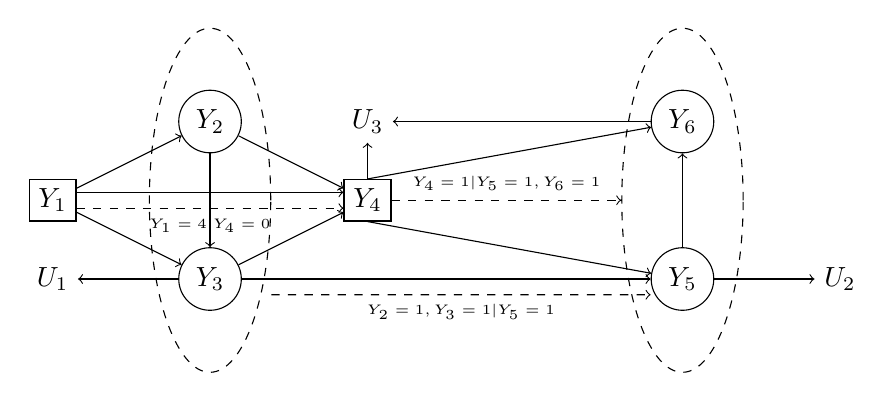
\begin{tikzpicture}[node distance=4cm]
\node[draw,rectangle] (00) at (0,0) {$Y_1$};
\node[draw,circle] (1-1) at (2,-1) {$Y_3$};
\node[draw,circle] (11) at (2,1) {$Y_2$};
\node[draw,rectangle] (20) at (4,0) {$Y_4$};
\node[draw,circle] (31) at (8,1) {$Y_6$};
\node[draw,circle] (3-1) at (8,-1) {$Y_5$};
\node (0-1) at (0,-1) {$U_1$};
\node (21) at (4,1) {$U_3$};
\node (4-1) at (10,-1) {$U_2$};
\draw[->] (00) -- (11);
\draw[->] (00) -- (1-1);
\draw[->,anchor=center, below] ([yshift=0.1cm]00.east) to node {} ([yshift=0.1cm]20.west);
\draw[->,dashed,anchor=center, below] ([yshift=-0.1cm]00.east) to node {\tiny{$Y_1=4|Y_4=0$}} ([yshift=-0.1cm]20.west);
\draw[->] (11) -- (1-1);
\draw[->] (1-1) -- (0-1);
\draw[->] (20) -- (21);
\draw[->] (31) -- (21);
\draw[->] (3-1) -- (4-1);
\draw[->] (11) -- (20);
\draw[->] (1-1) -- (20);
\draw[->] (1-1) -- (3-1);
\draw[->,anchor=center, below] (20.north) to node {} (31);
\draw[->,anchor=center, below] (20.south) to node {} (3-1);
\draw[->] (3-1) -- (31);
\node[draw=black, dashed, ellipse, inner sep =4pt, fit= (11) (1-1)] (circ1) {};
\node[draw=black, dashed, ellipse, inner sep =4pt, fit= (31) (3-1)] (circ2) {};
\draw[->, dashed,anchor=center, below] ([yshift=-1.2cm]circ1.east) to node {\tiny{$Y_2=1,Y_3=1|Y_5=1$}} ([yshift=-0.2cm]3-1.west);
\draw[->, dashed,anchor=center, above] (20) to node {\tiny{$Y_4=1|Y_5=1,Y_6=1$}} (circ2.west);
\end{tikzpicture}
\end{center}
\vspace{-0.4cm}
\caption{Representation of the asymmetric version of the multiplicative influence diagram of Figure \ref{fig-ex} as a sequential influence diagram. }\label{sid}
\end{figure}

Our graphical representation of these asymmetries is given in Figure \ref{sid}, corresponding to a sequential ID \citep{Jensen2006}. Asymmetries are represented as labels on additional dashed arcs. If the asymmetry is composite, meaning that it involves more than two variables, then vertices can be grouped through a dashed ellipse and dashed arcs can either start or finish by the side of these ellipses. As exemplified by the diagram in Figure \ref{sid}, the graphical representation of asymmetric decision problems, although providing a framework to quickly identify optimal policies, often lose the intuitiveness and the clarity of representation of standard IDs. We discuss more extensively this issue in Section \ref{sec:symbolic}. 

Asymmetric decision problems can also be explicitly modelled as \textit{decision trees} \citep[see e.g.][]{Clemen1996a,French2009}, an augmented version of an event tree including decision vertices and whose leaves are utilities. These suffer the same drawbacks of staged and event trees. Recently \citet{Cowell2010} introduced the decision CEG which can more compactly represent asymmetric decision problems.
 
\section{Group Decision Making}
\label{sec:group}
The SEU model characterises rational decision making for single DMs. However, in practice, most decisions in organisations and society are the responsibility of groups rather than individuals: juries, cabinets and boards of directors are some examples. In addition, even single DMs rarely commit to certain courses of actions without seeking for the help of appropriate experts. How the suggestions of various experts have to be reconciled is a very interesting question and a variety of solutions have been proposed. Following \citet{French2011}, we identify two main contexts of group decision making:
\begin{itemize}
\item the \textbf{group decision problem}: a group of individuals is jointly responsible and accountable for the decision;
\item the \textbf{expert problem}: a group of experts are consulted by a single DM who is responsible and accountable for the decision to be made.
\end{itemize}
\citet{French2011} also identifies the \textit{textbook problem} context which for the purpose of this thesis is not discussed here. Note further that a combination of the two above scenario can be considered in practice. There are two main categories of approaches for both contexts: behavioural and mathematical. We review the former ones in Section \ref{sec:decconf}.

Mathematical approaches for the group decision problem are based on some algorithmic rule which, given the preferences and beliefs of each individual DM, then outputs the decision ranking of the group. We do not focus in this thesis on these methods and we simply note here that there is vast literature about these \citep[see e.g.][]{Arrow1963,Keeney1976, Keeney1993a, French2009,French2011,Keeney2013}. Most of these methods, embedding some idea of democratic voting, are subject to paradoxes and inconsistencies. We discuss mathematical approaches for the expert problem in Section \ref{sec:expert}.
 
\subsection{Behavioural Approaches}
\label{sec:decconf}

\textit{Decision conferences} and \textit{facilitated workshops} are the most common techniques of behavioural aggregation of DMs' beliefs and preferences \citep{ Ackermann1996,Phillips1984,Phillips1993}. These are usually two days events with around fifteen participants \citep[although for example in the Chernobyl project we discussed in Chapter \ref{chapter1} the number of participants was way larger, as noted in][]{French2009}. In such meetings, a \textit{facilitator}, an individual skilled in the process of group discussion, encourages debate among the DMs and keeps the group's focus on the issue at hand. The facilitator is usually not an expert of the problem to be examined and has no ownership of the decision to be made. Each DM often has available interactive software to run her own analyses and observe the results of others' beliefs, which are also projected in the room. This software uses decision models which turns out to be fundamental to foster discussion and raise the main issues that need to be investigated by the group. The results of sensitivity analyses are also shown to the DMs in order to build consensus and avoid debates on irrelevant alternatives or parameters that do not affect the group's course of action. 

As discussed in Chapter \ref{chapter1}, these types of meetings were central to the decision elicitation process within the Chernobyl Project. The discussions at those meetings are summarised in \citet{French2009} and \citet{Smith2010}. \citet{Ackermann1996} reports more than 100 of successful applications of such behavioural techniques. 

A different method called \textit{Delphi protocol} has been designed to reach consensus by the remote and electronic compilation of a series of questionnaire, thus not requiring the group to meet \citep{Dalkey1963,Linstone1975}. Under this protocol, each individual anonymously responds to the questionnaire. The answers are then sent to the other members for further comments and generations of possible courses of actions. This sequence is then iteratively repeated until consensus is reached. 
 
\subsection{The Expert Problem}
\label{sec:expert}

The second context where groups are involved in the decision making process is the expert problem. Here an individual DM needs to synthesise the beliefs of a group of $m$ experts into a unique probability distribution. Mathematical methods for the aggregation of expert judgement can be broadly categorised into two main branches: Bayesian and pooling operator methods. Before discussing these approaches, we remark that it is not the scope of this thesis to explore the validity of each of these \citep[see e.g.][and the references therein for an extensive discussion]{Clemen99,French2011}. \citet{O'Hagan2006a} discussed protocols to be followed by each expert to elicit his own probability distribution, whilst \citet{Merrick2008} introduced methods to identify the right mix of experts to obtain the best aggregated belief. Here we mostly focus on pooling operators and we simply note that the Bayesian approach treats experts' judgements as data, synthesised in some appropriate likelihood function, to update the prior probability of the DM \citep[see e.g.][]{French1980, Mumpower1996,Wiper1995c,Albert2012}.

\subsubsection{Pooling Operators.}
\label{sec:pool}
Given the individual probabilities of a group of $m$ experts, $f^i(\bm{y})$, $i\in[m]$, pooling operators consist of a function  $T^p$ which pools together into a unique probability distribution, $f^{DM}(\bm{y})$, the probability distributions of each member of the group. For ease of notation we suppress the dependence on the parameter vector.

The simplest operator is the \textit{linear} one \citep{Stone1961}, corresponding to a weighted average of the experts' distributions:
\begin{equation*}
\label{eq:linearpool}
f^{DM}(\bm{y})=\T^p(f^1(\bm{y}),\dots, f^m(\bm{y}))=\sum_{e\in[m]} w^ef^e(\bm{y}).
\end{equation*} 
\citet{Bacharach1975} introduced the \textit{logarithmic Operator (logOp)} defined as
\begin{equation*}
\label{eq:logpool}
f^{DM}(\bm{y})=\T^p(f^1(\bm{y}),\dots, f^m(\bm{y}))\propto\prod_{e\in[m]}f^e(\bm{y})^{w^e}.
\end{equation*}

One of the main issues concerning pooling operators is the identification of the weights $w_e$ to be given to each expert. The aggregation most commonly used in practice is through a linear operator whose weights are calibrated according to the forecasting performance of the experts on a calibration set of uncertain quantities. This method is usually called \textit{classical} approach to the combination of expert judgements \citep{Cooke1991a}.

Sets of axioms characterising operators encoding rational behaviour have been defined \citep[see for a review][]{Genest86}.  We argue here, following \citet{Faria1997}, that one very desirable property for a pooling operator is to be \textit{Externally Bayesian (EB)} \citep{Madansky64}. 
\begin{definition}
A pooling operator $\T^p$ is said to be EB if  $f^{DM}(\bm{y})$ is the same when the following two procedures are implemented:
\begin{itemize}
\item first apply $\T^p$ and then update $f^{DM}(\bm{y})$ using Bayes theorem;
\item first update each expert's distribution $f^i(\bm{y})$ via Bayes Theorem and then apply $\T^p$. 
\end{itemize}
\end{definition} 
Therefore for EB operators the order in which pooling and updating are performed is irrelevant. This is a desirable property for a variety of reasons: first, experts do not need to meet every time data is collected; second, experts cannot increase their influence on the outcome by choosing whether to include their beliefs before or after the collection of data; lastly, as we discuss below, operators exhibiting such a property are in general  able to retain the conditional independences underlying an agreed model.  Importantly, \citet{Genest84} characterised the logOp as the only operator being EB.
Although EB operators have useful properties in the domains we are addressing, we note that these operators have been criticised in the literature \citep[see e.g.][]{Lindley1985}.

\subsubsection{The Multivariate Case.}
When experts have to elicit probabilities in large multivariate settings, their performance might dramatically decrease because of the difficulty in assessing correlations \citep{Clemen2000,Winkler2004}. One approach often used to mitigate such difficulties is to elicit probabilities over an agreed qualitative graphical structure, as for example a BN \citep{Burns1993, Faria1997, Farr2015, Renooij2001,Smith2000}. \citet{Smith1996a} extensively argued that experts' agreement can be more easily found in graphical frameworks since the underlying conditional independence structure can be discussed in natural language.

 \citet{Pennock2005} proved that a pooled distribution obtained with a logOp reflects any shared Markov independence by the group and for this reason, it can be represented in a concise and natural manner with a BN as well. However, it was also noted that no pooling operator can maintain all independences representable in a BN. Having acknowledged this negative result, in Chapter \ref{chapter3} we develop a framework where groups of experts qualitatively agree on a specific graphical model and then quantitatively individually deliver probability judgements, preserving the group's conditional independence structure. 
 
 Here we focus on the work of \citet{Faria1996} and \citet{Faria1997} which assumes the presence of an underlying decomposable CG agreed by all the experts. Their work, introducing a generalisation of the logOp, falls within the pooling operators approach. Suppose the decomposable CG $\Gr$ has $n$ chain components $\{\bm{Y}_i:i\in[n]\}$ .
 
\begin{definition}
For a decomposable CG $\Gr$, the \textbf{conditional logOp}, $\T^P$, is defined by the components $\T^p_{\Pi_j}$ 
\begin{equation*}
\label{eq:clogop}
f^{DM}_j(\bm{y}_j\;|\;\bm{y}_{\Pi_j})=\T^p_{\Pi_j}(\cdot)\propto \prod_{i\in[m]}f_{j}^i(\bm{y}_j\;|\; \bm{y}_{\Pi_j})^{w_{j}^i(\Pi_j)},
\end{equation*}
where $f_{j}^i$ is is the conditional density relative to $\bm{Y}_j$ provided by the $i$-th expert and $w_{j}^i(\Pi_j)$ is a weight. The DM distribution is then defined as
\begin{equation*}
f^{DM}(\bm{y})=\T^p=\prod_{j\in[n]}\T^p_{\Pi_j}=\prod_{j\in[n]}  f^{DM}_j(\bm{y}_j\;|\;\bm{y}_{\Pi_j}).
\end{equation*}
\end{definition}

Although the conditional logOp is not EB, \citet{Faria1997} showed that it respects a weaker condition called Conditional External Bayesianity (CEB). 

\begin{definition}
Given a CG $\Gr$, \textbf{CEB} holds if the conditional densities $f_{j}^i(\bm{y}_j\;|\; \bm{y}_{\Pi_j})$, $i\in[m]$, $j\in[n]$, are pooled with an EB operator.
\end{definition}

We define here a class of likelihood functions that guarantees CEB when the pooling is performed with a conditional logOp.

\begin{definition}
\label{def:cutting}
A likelihood $l(\bm{x}\;|\;\bm{y})$ for a sample $\bm{x}^\T=(\bm{x}_i)_{i\in[n]}$ is in the class of \emph{cutting} likelihoods of a CG $\Gr$ with chain components $\{\bm{Y}_i:i\in[n]\}$ if
\begin{equation}
l(\bm{x}\;|\;\bm{y})=l_1(\bm{x}_1\;|\;\bm{y}_1)l_2(\bm{x}_2|\bm{y}_2, \bm{y}_{\Pi_2},\bm{x}_1)\cdots l_n(\bm{x}_n\;|\;\bm{y}_n,\bm{y}_{\Pi_n},\bm{x}^{n-1}).
\label{eq:cutting}
\end{equation}
\end{definition} 

\citet{Faria1997} then proved that the conditional logOp respects CEB when the pooling/updating is performed according to a procedure we briefly review here. Let $\tilde{f}_g$ be the joint density over $\Gr$ obtained by first pooling the individual posterior densities on $\bm{Y}_n\;|\; \bm{Y}_{\Pi_n}, \bm{X}$, then using the derived density on $\bm{X}\;|\; \bm{Y}^{n-1}$ to pool the  individual posteriors on $\bm{Y}_{n-1}\;|\;\bm{Y}_{\Pi_{n-1}},\bm{X}$, and so on. Conversely, let $\bar{f}_g$ the joint density over $\Gr$ obtained by first pooling the individual prior densities on $\bm{Y}_{n}\;|\;\bm{Y}_{\Pi_n}$ and forming the group's posterior density of $\bm{Y}_n\;|\;\bm{Y}_{\Pi_n},\bm{X}$, then pooling the individual priors on $\bm{Y}_{n-1}\;|\;\bm{Y}_{\Pi_{n-1}}$ and forming the posterior on $\bm{Y}_{n-1}\;|\;\bm{Y}_{\Pi_{n-1}},\bm{X}$ using the density of $\bm{X}\;|\;\bm{Y}^{n-1}$, and so on. We say that when these procedures are followed, the densities are \textit{backward sequentially updated}. It is apparent that an operator respecting CEB is such that $\tilde{f}(\bm{y}\;|\; \bm{x})=\bar{f}(\bm{y}\;|\;\bm{x})$.

\begin{proposition}
\label{prop:ceb}
The conditional logOp respects CEB for a decomposable CG $\Gr$ when distributions $f_{i}^j(\cdot)$ and $f^{DM}_i(\cdot)$, $i\in[n]$, $j\in[m]$, are backward sequentially updated.
\end{proposition}
 
 In Chapter \ref{chapter3} we discuss a variation of this result to cases where different groups of experts are responsible for disjoint subsets of the vertices of the CG. Furthermore, in Chapter \ref{chapter4} we develop recursions in dynamic settings which mirror the backward 
sequential updating of \citet{Faria1997}. 

\subsubsection{Aggregation in Complex Problems.}
The previous sections considered situations where experts can simply provide probabilities, possibly in a multivariate setting, for the whole domain under study. However, as we have extensively argued, in the applications we have in mind this can be only rarely  the case. A first attempt to generalise such framework for expert judgement combination was proposed in \citet{Bordley2009}. In that paper each expert delivers probabilities over a separate, but related, set of events and aggregating methods are then developed to reconcile their judgements into a unique probability distribution.

In complex applications however, experts can rarely simply  deliver  numbers representing their estimates and the uncertainty around these. They often run their own models and observe their outputs to then deliver the required uncertainties \citep{French2011}. This should be apparent from the RODOS discussion in Chapter \ref{chapter1}. This issue was already noticed in nuclear emergency management in \citet{Cooke2000}. The ENSAMBLE project \citep{Krishnamurti2000,Mikkelsen2003} is another example of this type of combination, where the outputs of different meteorological models need to be combined into a unique weather forecast. These types of combinations introduce new challenges since correlated estimates and uncertainties may arise at both  the expert and the model level. 

\citet{French2011} pointed out that the issue becomes even more delicate when models need to be chained together as in the RODOS modules' structure exemplified in Figure \ref{networkino}. Very little has been said on this issue and some early discussion on possible solutions were proposed in \citet{French1991}.  In the following chapters we explicitly address these types of problems and define a framework to coherently network together models and expert judgements.
 
\section{Conclusions and Contributions}
This chapter has summarised the main aspects of the Bayesian approach to inference and decision making that are relevant for this thesis. We have reviewed a variety of methods to represent both the uncertainties and the preferences of individual DMs. However we have noted that current methods for groups of DMs and for combining the judgements of several experts in complex domains are limited. In the following chapters we extend  Bayesian methodology to allow for a coherent aggregation of experts' beliefs and preferences in complex domains. We are able to show that many of the graphical models we have introduced provide an intuitive basis to do this. 

Note that some of the concepts introduced in this chapter, namely directional utility diagrams, MIDs and their evaluation are original contributions to the literature. We discuss additional features of these models in the following chapters. 

\subsection{Contributions}
Having introduced in details the normative framework of Bayesian decision analysis and inference, we can now discuss more explicitly the contributions of this thesis to the literature. To increase readability, we discuss the extensions we propose in the same order as in the list on pages 13-14.
\begin{itemize}
\item in this chapter we have shown how probabilistic inference can be carried in a distributed fashion for a variety of models when certain independences are assumed for the model parameter vector (specified in Definition 2.3.9 for BNs, in Definition 2.3.21 for MNs, on page 39 for CEGs and in Proposition 2.3.39 for MDMs). In Section 3.6 we introduce weaker conditions for these models, enabling distributed inferences when different panels of experts deliver the required probabilities for disjoint subsets of the vertex set of the underlying graph;
\item  the combination rules for expert judgements of \citet{Faria1997} briefly reviewed in Proposition 2.6.5 work when each expert deliver probabilities for every variable of an underlying CG. We extend this result in Section 3.6 to cases where experts deliver judgements only for subsets of the graph's vertex set;
\item in Section 2.3.4 we introduced the Perlean notion of causality and discussed Perlean intervention in Definition 2.3.49. In Section 3.5 below we introduce a new notion of causality extending the one of Pearl in two ways: first, our definition does not require the existence of an idle system, but instead assumes the existence of a natural comparator - a decision rule which is standard in the domain examined;  second, it allows for more general interventions than the \lq{d}o\rq \;  standard operator;
\item Definition 2.4.23 introduced bidirectional utility diagrams, a flexible graphical representation of partial utility independence. In Chapter 4 (and specifically Definition 4.1.8 and Proposition 4.1.10) we introduce a particular subclass of these models and deduce the utility factorization associated to this subclass. Such a class, together with a few other assumptions often made in practice (see Section 4.1), we enables the distributed computation of expected utility $\bar{u}(\bm{d})$ of any policy $\bm{d}$ as discussed in Theorem 4.1.13;
\item the computation of the expected utilities for utilities in the class mentioned in the previous point  can be carried using a backward induction procedure which mirrors the routine of \citet{Faria1997} to pool probability distributions (explicated on page 72); in Chapter 4 we introduce new backward inductions that instead of pooling probability distributions, compute optimal expected utility in multi-expert domains; 
\item in Section 2.1.2 we introduced moments and discusses their role in summarizing the features of a distribution. \citet{Cowell1999a} and \citet{Nilsson2001} introduced closed form recursions to compute moments of additive factorizations, as the ones in Proposition 2.4.16, over a BN model. In Chapter 5 we generalize such recursions to compute moments for multilinear factorizations introduced in Proposition 2.4.11;
\item standard conditional independence, as discussed in Section 2.3.1., often implies separations between certain functions of the model's parameter that are not strictly required for the computation of the  moments mentioned in the point above. In Section 5.3 we introduce new separation conditions, often implied by conditional independence, allowing for the computations of the above moments;
\item we define new symbolic inferential techniques in CEG and ID models, extending current methods for discrete BNs. For these models, each entry of a probability table, $\theta_i$ say, is considered as an indeterminate of a polynomial (or equally as a variable in a computer algebra system) and inference is carried with no full numerical specification of the model's probabilities. For CEGs, we extend current methods from symmetric to asymmetric probabilistic models. For IDs, we introduce a symbolic definition of utility values and introduce the polynomial form of the expected utilities associated to these models.   
\end{itemize} 

\chapter{The Integrating Decision Support System} % Main chapter title

\label{chapter3} % For referencing the chapter elsewhere, use \ref{Chapter1} 

\lhead{Chapter 3. \emph{The integrating decision support system}} % This is for the header on each page - perhaps a shortened title

The probabilistic decision support techniques for single users we reviewed in Chapter \ref{chapter2} have many advantages: these are coherent from a Bayesian viewpoint and can embed expert judgement when necessary. However the types of demands of current applications, such as the nuclear one we reviewed in Section \ref{sec:nuclear}, require new methods to coherently combine the outputs of networked experts systems in order to provide an integrated study of the whole domain. Therefore, as argued in Chapter \ref{chapter1}, what is needed is an integrating DSS, taking very selected probabilistic outputs from each contributing module and pasting these expert judgements together to provide a comprehensive support. 

We report in this chapter the results of \citet{Smith2015} where we developed a sound statistical methodology to underpin such an integrating system. This provides a framework to faithfully encode all usable and informed expert judgements and data leading to the production of numerical scores ranking the available policies. We envisage that either any of the models we reviewed in Section \ref{sec:prob} or one of the many large
scale hierarchical Bayesian models of temporal spatial processes now in place \citep[e.g.][]{Best2005,Jewell2009, McKinley2014, Wikle2001} informs one of the components of the IDSS. Each of these modules, drawing on experimental and observational evidence supplemented by expert judgement, either directly informs arguments of a decision centre's utility function or provides the necessary input to subsequent components in the process. Different panels of experts in the domain defined by each component oversee and are responsible for the probabilistic outputs of the particular component capturing part of an underlying process. The IDSS is then designed to draw these probabilistic judgements into a single coherent picture to inform policy making. Such a coherent IDSS would thus embody all the qualitative common knowledge and fully defensible domain knowledge of the different panels, and provide baseline judgements around which discussions and modifications could be proposed. 

We describe here how and when it is possible to build such an IDSS and develop statistical methodologies to appropriately guide this knowledge integration. We first introduce a new set of axioms embedding the agreement the group of experts needs to find and, generalising results from \citet{Goldstein96}, we show that these can guarantee the existence of a coherent IDSS. We then define new group Bayesian updating routines for both observational and experimental data for cases where the IDSS is underpinned by a new notion of statistical causality. Lastly, we generalise both current independence conditions and inferential methods for single DMs to groups in a variety of graphical model classes.

The chapter is organised as follows. In Section \ref{sec:features1} we briefly discuss the features of IDSSs and the possible types of support such systems can provide. Section \ref{sec:construction} builds the IDSS methodology and discusses some technical properties that IDSSs need to entertain. In Section \ref{sec:idssexamples} we present some very simple illustrative examples to show the difficulties and the inconsistencies that IDSSs may exhibit.  Section \ref{sec:conditions} presents a number of results that ensure a coherent and faithful IDSS both a priori and after the introduction of observational data. In Section \ref{sec:idsscaus} we then introduce a definition of causality tailored to IDSSs and show that  experimental evidence can be accommodated in these systems whilst retaining coherence. In Section \ref{sec:idssex} we demonstrate that most of the models we reviewed in Sections \ref{sec:nondym} and \ref{sec:dynmod} can be used as integrating overarching structure to aggregate the diverse expert systems' outputs. We conclude with a discussion. 
 
\section{Features of Integrating Systems}
\label{sec:features1}

The description of the RODOS system in Section \ref{sec:nuclear} highlighted the need in current applications for systems capable of drawing different components of the problem together. The IDSS methodology aims at supporting decision centres using expert judgement coming from different panels with different knowledge. We call the \textit{collective} the totality of the experts in the panels, potential users and relevant stakeholders. The IDSS embeds a particular type of \lq{group}\rq ~decision analysis where everyone in the collective accepts to delegate a particular aspect of the problem to the most informed experts  only. The features of this type of decision analysis are summarised in Figure \ref{diagramma}. The collective agrees on the overarching, meaning across panels, probabilistic, preferential and decision structure of the problem the IDSS addresses, as specified by the top three boxes of the diagram in Figure \ref{diagramma}. By overarching statistical model, we mean that the collective identifies the main variables of the problem and the input/output relationships between these, described, for instance, by a set of conditional independence statements or by a graphical model as the network in Figure \ref{networkino}. On the other hand, a preferential overarching model consists of the identification of the attributes of the domain under study together with a set of preferential independences represented, for instance, by a specific utility factorization. In both cases no actual probability and utility elicitations are performed. Then each panel builds its own probabilistic and preferential models, only concerning the domain under its responsibility. These are then integrated into a unique entity to rank policies according to their expected utilities to provide decision support, as indicated by the bottom boxes in Figure \ref{diagramma}.
\begin{figure}
\begin{center}
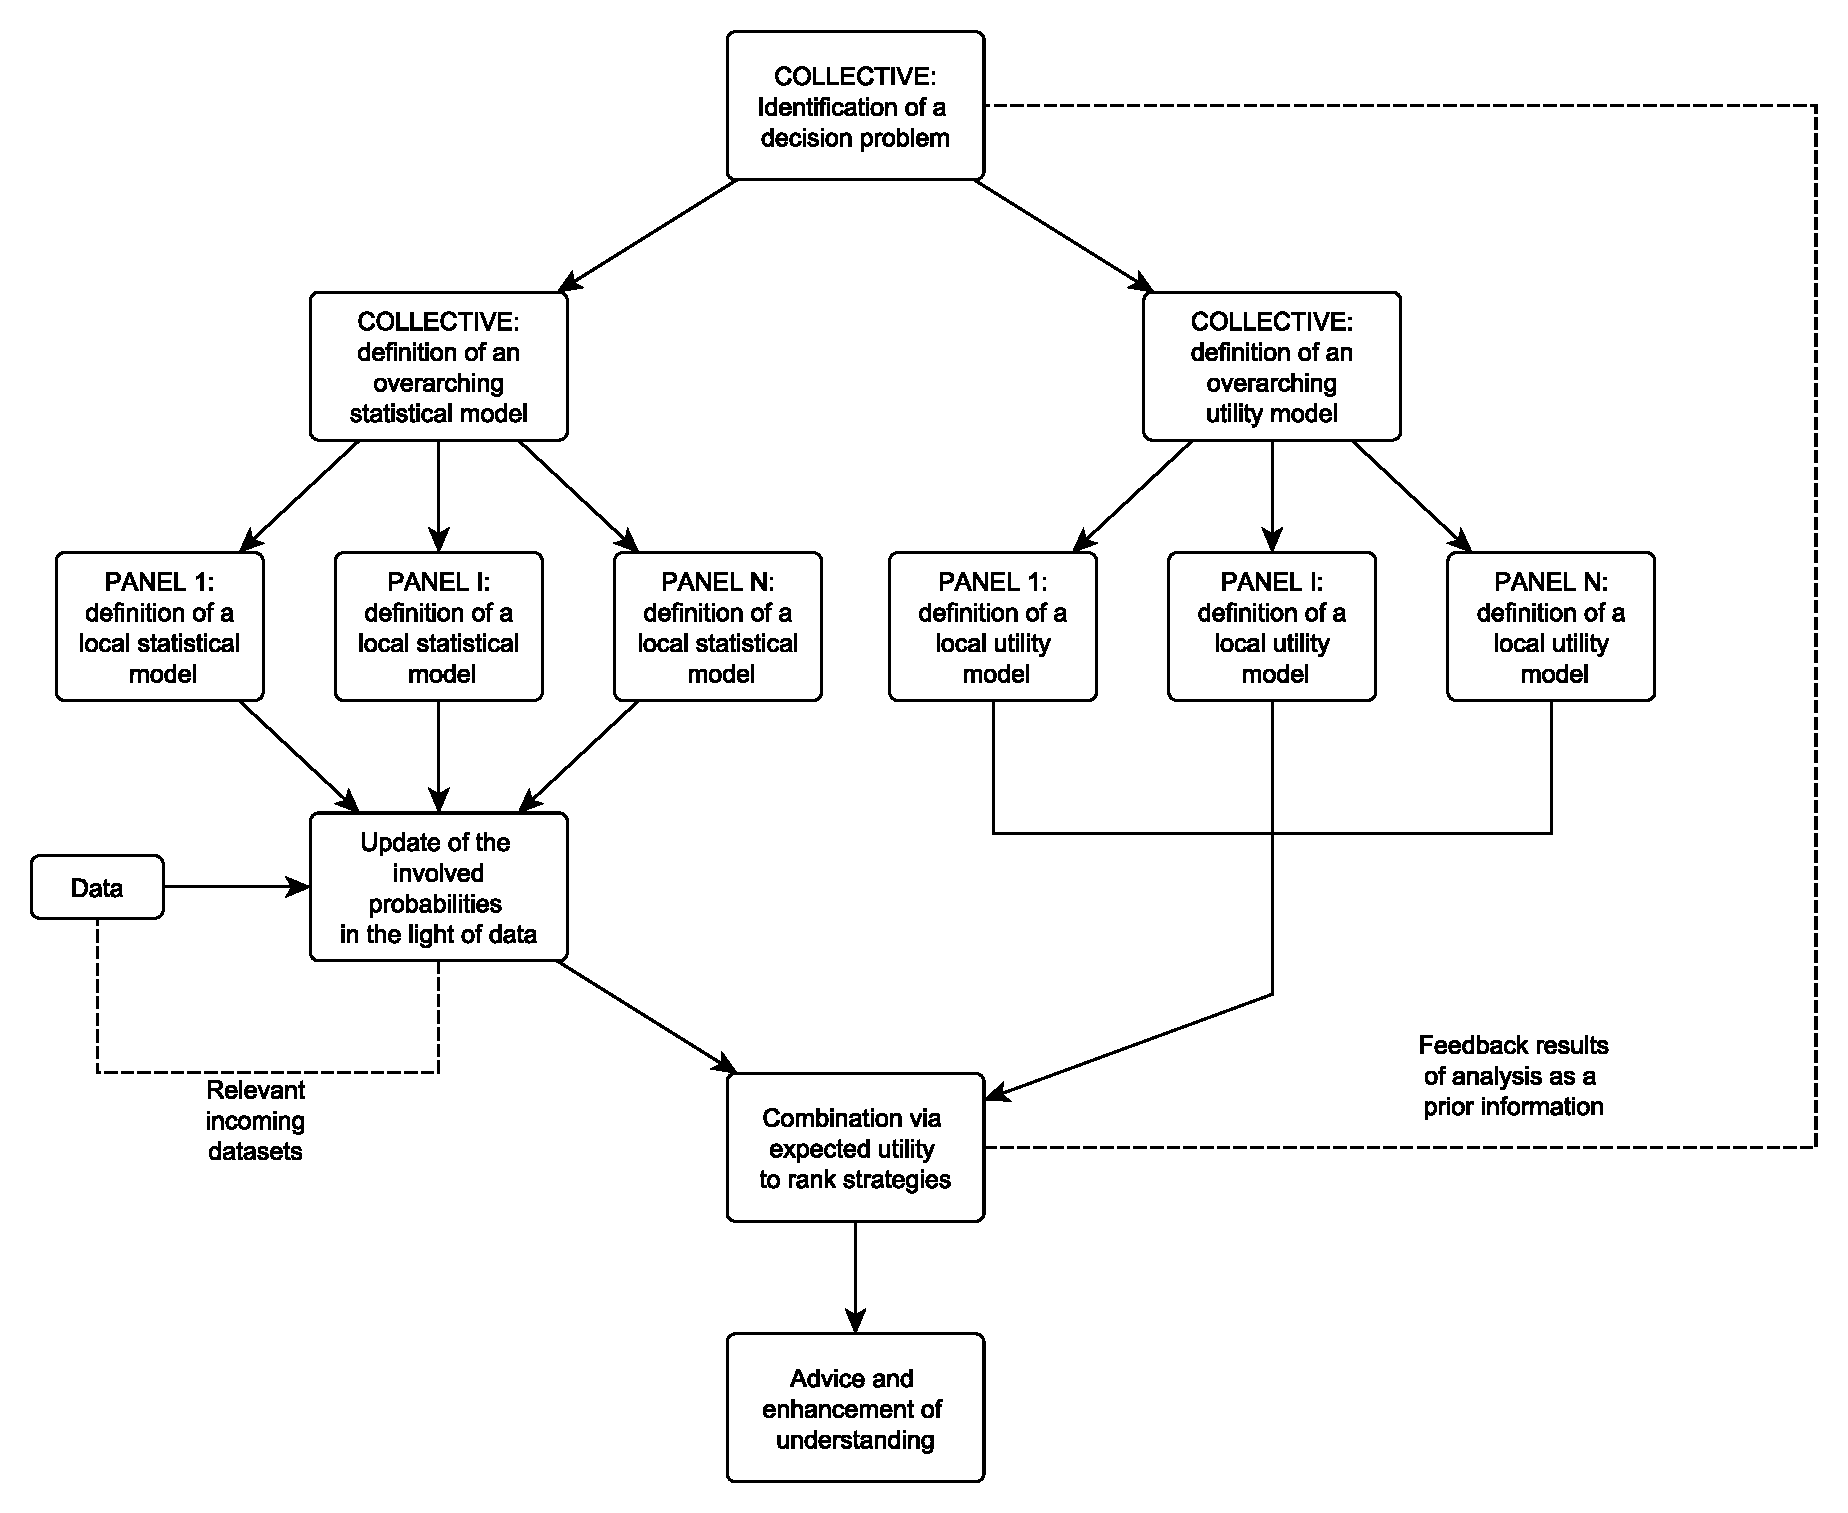
\includegraphics[scale=0.45]{Figure2}
\end{center}
\caption{Structure of a Bayesian decision analysis for a group of distributed experts from \citet{Leonelli2015}, generalising \citet{French97}. \label{diagramma}}
\end{figure}

 One of the challenges to  this process of integration is that no one person or group owns all the relevant probabilistic expert judgements. A first and essential requirement for an IDSS is that its suggestions need to be defensible to the challenges a decision centre might face to the validity of any analysis it might produce. Inputs and outputs of the subsystems and specifically the associated expressions and balancing of uncertainty need not to be self contradictory with each other. Within a Bayesian paradigm this is a \textbf{coherence} requirement over the variables determining the overall expected utility scores, corresponding to the formal separability condition of \citet{Mahoney1996} discussed in Chapter \ref{chapter1}. In a nutshell, this entails that it is possible to define a unique probability distribution over the complete system given the beliefs of the panels. For example if  probability distributions are assigned by two different panels to the amount of contamination to the ground and in water respectively, which have within them an assessment of the air dispersal of contamination, then this assessment has to be the same for the two distributions. If this were not the case, a unique distribution over the IDSS could not be computed and the credibility of the composite would be clearly compromised. 

A second requirement for a practical IDSS is that the panels deliver \textit{sufficiently rich} sets of information, so that they together provide enough information to compute the expected utility function. This is in general impossible unless some assumptions are made by the collective. Note that some parts of the process under examination may be very well studied and modelled, but the knowledge about others is often patchy. So for instance, dispersal models are now well established and able to compute a variety of summaries  of the spread of contamination, whilst the estimates of the political effects of the accident on the stability of the affected regions often come only in the form of expert judgement.  

A third important property increasing the defensibility of the outputs of an IDSS is that this incorporates the \textit{fullest} and \textit{most reliable} possible \textit{evidence} within its probability specifications. This in turn requires that expert judgements are provided only by the most informed panels. However, IDSSs that are coherent a priori might not be so any more after the introduction of data. For this reason, filters checking the data that is admitted in the IDSS to perform Bayesian updating need to be implemented. If these filters are in place, then panels can produce revised estimates of the required quantities for the decision analysis, improving the overall suggestions the system is producing and consequently supporting more focused decision making. 


It is also often necessary for the IDSS to be used in real time, during the unfolding of a certain crisis. Modules are now designed so that they are fast. However this is not sufficient to guarantee that the composite as a whole is able to run quickly and still retain its coherence. To achieve this, a necessary property is that the system is \textbf{distributed} (or \textit{modular}). By this we mean that the composite system calculates all functions needed to evaluate the expected utility associated with its available decisions from outputs delivered by individual panels, where these are allowed to be functions of other panels' outputs. There are several advantages that derive from structuring a problems so that the ensuing support is distributed:
\begin{enumerate}
\item first, because the responsibility for each aspect of the analysis can be devolved to \textit{appropriate} panels of experts, these are then more likely to deliver better calibrated judgements.  This in some ways guarantees the semantic separability of \citet{Mahoney1996}. The whole system might therefore be expected to be more robust to the misspecification of beliefs \citep{Cooke1991a}. On the other hand, if the system needs to be changed in the light of unexpected developments or unplanned consequences, under suitable conditions, the management of these new developments need only be addressed \textit{autonomously} by the relevant panels. These simply adapt their individual forecasts and inputs in the light of the new scenario they face. These adjustments can then be folded back into the system to provide  a revised output of the relevant modules for other panels to use for their inputs;
\item second, the output of a distributed IDSS can produce answers to queries by decision centres about the premises on which it is based and the calculations of its outputs, by directing the query to the relevant panels. A route along which the relevant panels can be queried as to the reasons of their contribution to the expected utility scores is described in Figure \ref{possuse}, which shows the different levels of support that can be implemented into an IDSS. When queried, generic DSSs are usually able to present justifications for the overall expected utility scores and the ranking of the available policies (third box of the second column from the left of Figure \ref{possuse}). However IDSSs are able to provide an additional level of support. The system's distributivity permits the IDSS to justify its suggestions in terms of the modules outputs, since expected utilities are functions of these (see the bottom box of the second column from the left of Figure \ref{possuse}). If these systems did not exhibit this distributivity property, then such devolution may not be possible and so any support would be much less transparent. This feature increases both the comprehensibility and the feasibility of testing that, as argued by \citet{Mahoney1996}, current DSSs need to address;
\item third, distributivity ensures that different decision centres can be given the option of choosing different modules to model the various components of the problem. For example, in nuclear emergency management, different countries often prefer to predict the spread of the contamination using  their national agencies' diffusion models;
\item lastly, although many of the modules are probabilistic, distributivity allows us not to construct a single composite probabilistic model: such a universal system would be infeasibly large and no one would own the joint distributions of the unwieldy number of random variables. Even if it were possible to build such a system, the component modules are usually being constantly revised both in their structure and inputs. Were such an overarching probabilistic system possible to build, it would therefore be obsolete before it was completed.  
\end{enumerate}

\begin{figure}
\begin{center}
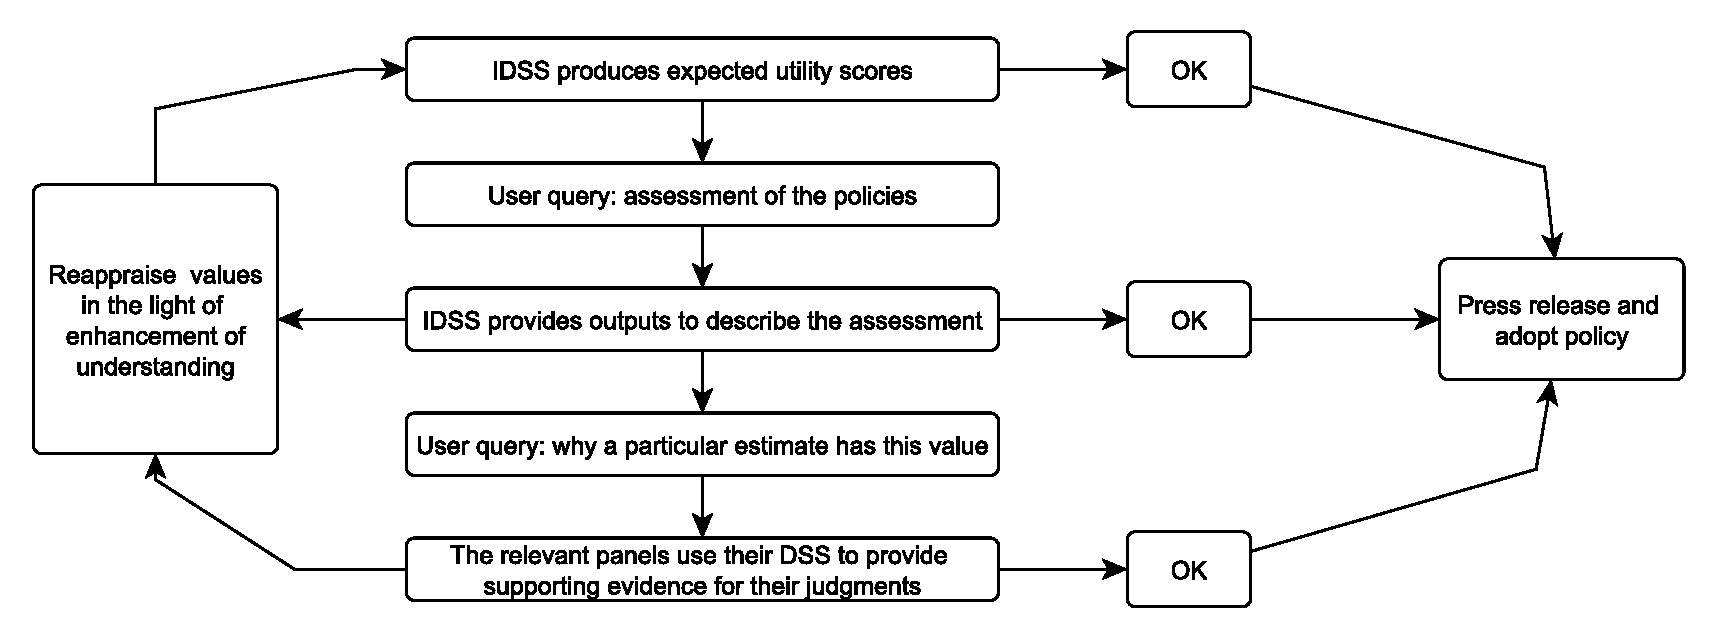
\includegraphics[scale=0.5]{Figure1}
\caption{Description of the possible use of an integrating decision support system for a decision analysis. \label{possuse}}
\end{center}
\end{figure}


\section{Construction of Integrating Systems}
\label{sec:construction}
\subsection{Some Technical Structure}
A domain is defined by a large number of random variables $\bm{Y}=(Y_i)_{i\in[n]}^{\T}$. As often in practice, the problem is heterogeneous and therefore assume different components of the problem, denoted as $\bm{Y}_i$, are evaluated and overseen by $m$ different panels $\{G_i: i\in[m]\}$ of domain experts, $[m]=\{1,\dots, m\}$. The implicit, albeit virtual, owner of these beliefs is henceforth referred to as the SB. Let $\bm{\mathcal{D}}$ be a decision space including the available policies $\bm{d}\in\bm{\mathcal{D}}$.  The SB needs to process the necessary probabilistic features delivered by the different panels to calculate various statistics of a potential decision centre's reward vector $\bm{R}$, some function of both $\bm{Y}$ and $\bm{d}$. 

Panel $G_i$ donates to the SB various summaries of the distribution of the subvector $\bm{Y}_i\;|\;\bm{d}$ under its jurisdiction, conditional on certain measurable functions $\{L_i(\bm{Y}_i):L_i\in\mathcal{L}_i\}$, where $\mathcal{L}_i$ could be empty, $i\in[m]$. For instance, in a generic graphical model the set $\mathcal{L}_i$ might consist of the possible configurations of values of the parents of $\bm{Y}_i$. Assume that panel $G_i$, $i\in [m]$, is able to make available the following:
\begin{enumerate}
\item a collection of summary statements about the measurements under its jurisdiction
\begin{equation*}
\Psi_i^{\bm{y}|\bm{\theta}}=\{\Psi_i^{\bm{y}|\bm{\theta}}(\bm{\theta}_i,L_i,\bm{d}): \bm{\theta}_i\in\bm{\Theta}_i,\;L_i\in\mathcal{L}_i,\;\bm{d}\in\bm{\mathcal{D}}\}.
\end{equation*}
These inform the IDSS about the likelihoods
$f_i(\bm{y}_{i}\;|\;\bm{\theta }_{i},L_i, \bm{d})$, $L_i\in \mathcal{L}_i$, $\bm{d}\in \bm{\mathcal{D}}$, where $\bm{\theta }_{i}\in \bm{\Theta} _{i}$ parametrise the (possibly conditional) density of $\bm{Y}_i\;|\;\bm{\theta},\bm{d}$. For example, if $\bm{Y}$ were discrete and finite, then each panel might be asked to provide certain contingency tables over $\bm{Y}_{i}\;|\;\bm{\theta},\bm{d}$, conditional on each $L_{i}\in \mathcal{L}_{i}$. In this case $\bm{\theta}_{i}\in \bm{\Theta} _{i}$ would be the probabilities within all these tables. An important note to make here is that there is often a typically much longer vector of parameters $\bm{\phi}_{i}\in \bm{\Phi} _{i}$ over which $G_{i}$ has beliefs but which are not directly relevant to the distribution of the predictions the IDSS needs to deliver;
\item a set of summaries about its prior beliefs  
\begin{equation*}
\Psi _{i}^{\bm{\theta} }=\left\{ \Psi _{i}^{\bm{\theta} }(L_i,\bm{d}): L_i\in\mathcal{L}_i,\;\bm{d}\in\bm{\mathcal{D}} \right\}, 
\end{equation*}
from the panel prior densities $\pi_i(\bm{\theta}_i\;|\;L_i,\;\bm{d})$, $\bm{d}\in\bm{\mathcal{D}}$, $L_i\in\mathcal{L}_i$. In the above example this would be a joint probability distribution over the entries of the relevant contingency tables. Note that often these panel beliefs are calculated by marginalising out $ \bm{\phi }_{i}\in \bm{\Phi}_{i}$;
\item from these two sets of quantities, the calculated collection of summaries 
\[
\Psi _{i}^{\bm{y}}= \left\{ \Psi _{i}^{\bm{y}}(L_i,\bm{d}):L_i\in\mathcal{L}_i,\; \bm{d}\in \bm{\mathcal{D}}\right\} ,
\]
about the marginal distribution of $\bm{Y}_{i}\;|\;\bm{d}$ conditional on each event $L_{i}$. Here $\Psi _{i}^{\bm{y}}(L_{i},\bm{d})$ is calculated from $\Psi_{i}^{\bm{y}|\bm{\theta }}(\bm{\theta }_{i},L_{i},\bm{d})$ by $G_{i}$ marginalising over $\bm{\theta }_{i}$ using $\Psi _{i}^{\bm{\theta}}(L_{i},\bm{d})$ for each $L_{i}\in \mathcal{L}_{i}$, $\bm{d}\in \bm{\mathcal{D}}$. In the example above, these might be the corresponding expected conditional tables where expectations are taken across the probability vectors $\bm{\theta }_{i}$.  These are the quantities the IDSS uses to calculate its expected utility scores associated with its available decisions and to help a decision centre to determine its most efficacious policy.
\end{enumerate}

\subsection{Common Knowledge Axioms}
Suppose that after a series of decision conferences (see Section \ref{sec:decconf}) held jointly across the panels, stakeholders and potential users, all have agreed the types of decisions the IDSS  supports to a sufficient level of specificity to provide an agreed qualitative framework across all interested parties around which a quantitative structure can be built. To this purpose we make three assumptions.

\begin{axiom}[policy consensus]
\label{axiom:policy}
The collective agrees the class of decision rules $\bm{d}\in \bm{\mathcal{D}}$ examined by the IDSS.
\end{axiom}

This class of feasible policies considered  depends not only on what is logical, such as when various pieces of information are likely to become available, but also what might be allowable, either legally or for other reasons.

\begin{axiom}[utility consensus]
\label{axiom:utility}
The collective agrees on the class $\mathcal{U}$ of utility functions supported by the IDSS.
\end{axiom}
In the complex multivariate settings we address here, the utility function $u(\bm{r},\bm{d})$ needs to entertain certain types of preferential independence in order to allow for a distributed analysis. In this chapter we assume that some additive or multilinear factorisation is believed to hold. In Chapter \ref{chapter4} we introduce a large class of partial utility independence models, of which additive and multilinear factorisations can be seen as a special case, that can allow for distributed analyses. Again the choice of $\mathcal{U}$ is often resolved using decision conferencing across the members of the collective.

\begin{axiom}[structural consensus]
\label{axiom:structural}
The collective agrees the variables $\bm{Y}$ defining the process - where for each $\bm{d}\in \bm{\mathcal{D}}$, each $u\in \mathcal{U}$ is a function of $\bm{Y}$ - together with a set of qualitative statements about the dependence between various functions of $\bm{Y}$, $\bm{\theta }$ and $\bm{d}$. Call this set of assumptions the \textbf{structural consensus set} and denote this by $\mathcal{J}$.
\end{axiom}
This last consensus might be expressible through agreement that a particular graphical or conditional independence structure across not only the distribution of $ \bm{Y}\;|\;\bm{\theta }, \bm{d}$,  but also over the one of $\bm{\theta }\;|\;\bm{d}$ is valid, $\bm{d}\in\bm{\mathcal{D}}$. For instance, the structural consensus might include the assumption of local and global independence of the parameter vector in a BN model (see Section \ref{sec:BN}). Other information that might be included in $\mathcal{J}$ could be a consensus about certain structural zeros or known logical constraints (such as probabilities needing to add to one and be non-negative).

\begin{definition}
Call the set of assumptions forming the union of the utility, policy and structural consensus $\left( \mathcal{U},\bm{\mathcal{D}},\mathcal{J}\right) $ the \textbf{Common Knowledge-class (CK-class))}.
\end{definition}

Technically, we can think of the CK-class as the \emph{qualitative} beliefs that are shared as common knowledge by all  panel members and potential users. The CK-class represents the foundation around which all inference within the IDSS takes place. Note that this depends not only on the domain and needs of users of the system, but also on the constitution and knowledge bases of the panels.

We now provide a list of the types of quantitative information needed to populate the CK-class and to calculate the expected utility $\bar{u}(\bm{d})$ of the available decisions $\bm{d}\in\bm{\mathcal{D}}$. To achieve this, the SB  needs the decision centre's choice of $u(\bm{r},\bm{d})\in \mathcal{U}$ together with enough probabilistic information to calculate the expectations of these utilities. At worst this might need to be the full distribution of $\bm{R}$. Alternatively and more commonly for typical choices of $\mathcal{U}$, all that might be needed is the distribution of the margins on certain specific functions of $\bm{R}$ or simply some summaries. 

\begin{axiom}[quantitative delegation consensus]
\label{axiom:quantitative}
The collective agrees to take on the sample summaries $\Psi _{i}^{\bm{y}|\bm{\theta} }$, the panel prior beliefs $\Psi _{i}^{\bm{\theta} }$ and the panel marginal inputs $\Psi _{i}^{\bm{y}}$ delivered by $G_{i}$ as its own, $i\in[m]$.
\end{axiom}
This axiom essentially demands that everyone agrees that it is appropriate to defer their judgements to the panel which is most informed about each domain vector. A sufficient set of qualitative conditions justifying its use is given in Section \ref{sec:coherence}.
\subsection{Properties of Integrating Systems}
The above axioms specify the structure of the IDSS, but these do not in general guarantee that the output of the system provides coherent decision support. In this section we introduce concepts that characterise what a \lq{good}' IDSS is.
\begin{definition}
\label{def:adequacy}
An IDSS is \textbf{adequate} for a CK-class if the SB can unambiguously calculate the expected utility scores, for any decision $\bm{d}\in \bm{\mathcal{D}}$ and any utility function $u\in \mathcal{U}$, from the panel marginal inputs $\Psi _{i}^{\bm{y}}$ delivered by $G_{i}$, $i\in[m]$.
\end{definition}
One particular useful refinement of adequacy is the following.
\begin{definition}
An IDSS is \textbf{universally adequate} for a CK-class if the SB can unambiguously calculate the distribution of $\bm{R}$ from the panel marginal inputs $\Psi _{i}^{\bm{y}}$ delivered by $G_{i}$, $i\in[m]$.
\end{definition}
An adequate IDSS is able to derive a unique score for each option on the basis of the individual panels' inputs. An IDSS clearly cannot be fully functional unless it has this property. For a universally adequate IDSS this is true regardless of the form of $\mathcal{U}$.

To be defensible the IDSS needs another property.
\begin{definition}
An IDSS is \textbf{sound} for a CK-class if it is adequate and the SB can coherently admit all the assessments $\Psi_{i}^{\bm{y}|\bm{\theta} },\Psi _{i}^{\bm{\theta }}$ and $\Psi _{i}^{\bm{y}}$, $i\in[m]$, as her own, the SB's underlying belief model being shared with those of the relevant panels.
\end{definition}
A sound IDSS does not necessarily need to embody the \emph{genuine} beliefs held by the panel members and potential users based on the totality of their own personal evidence. This would be too much to ask since much of this evidence might be from poorly designed experiments, formally unjustifiable to the public or simply anecdotal. However the sound IDSS does present a defensible and conservative position all panellist should be happy to communicate, and provide a benchmark for further discussion. Most importantly soundness guarantees that the beliefs are formally separable.

A property we  always assume to be part of a CK-class is that panels are variationally independent, i.e $\bm{\Theta}=\bigtimes_{i\in[m]}\bm{\Theta}_i$ (see Definition \ref{def:varind}). If this were not the case, then beliefs of one panel would be necessarily shared with the ones of other panels. In such case both soundness and distributivity could not hold for IDSSs.

\section{Illustrative Examples}
In this section we present a series of simple and intuitive examples illustrating the IDSS machinery and the dangers associated to non coherent belief specifications. 

\label{sec:idssexamples}
\subsection{Strong Adequacy and Soundness a Priori.}
Let $m=2$, $\bm{R}=\bm{Y}=(Y_1,Y_2)^\T$, where $Y_i$ is binary, $i\in[2]$, $\bm{\theta}$ parametrise the density of $(Y_1,Y_2)\;|\;\bm{\theta},\bm{d}$, and suppose a generic decision space $\bm{\mathcal{D}}$.  Here the random variable $Y_1$ is an indicator of whether or not the contamination is dispersed in the area and $Y_2$ is an indicator of whether or not the population is affected by the accident. The sample summary delivered by $G_1$  is $\theta_1=\mathbb{P}(Y_1=1\;|\;\theta_1,\bm{d})$, whilst $G_2$ delivers $\{\theta_{20},\theta_{21}\}$, where $\theta_{20}=\mathbb{P}(Y_2=1\;|\;Y_1=0,\theta_{20},\bm{d})$ and $\theta_{21}=\mathbb{P}(Y_2=1\;|\;Y_1=1,\theta_{21},\bm{d})$.   Write $\bm{\theta}_2=(\theta_{20},\theta_{21})^\T$. Note that in this case $\mathcal{L}_1$ is empty, whilst $\mathcal{L}_2$ consists of the possible outcomes of $Y_1$.

  If a CK-class includes $\mathcal{U}$, an arbitrary utility on $\bm{R}$, then, since the above probabilities fully define the model, for strong adequacy the SB needs to be able to calculate the expected joint probability table of $\bm{Y}\;|\;\bm{d}$. Specifically this corresponds to the expected values $\bar{\bm{\mu }}=( \bar{\mu }_{00},\bar{\mu }_{01},\bar{\mu }_{10},\bar{\mu }_{11})^\T $ of $\bar{\bm{\theta }}=( \bar{\theta }_{00},\bar{\theta }_{01},\bar{\theta }_{10},\bar{\theta }_{11})^\T $, where by definition 
\begin{equation*}
\begin{array}{cccc}
\bar{\theta }_{00}=(1-\theta _{1})(1-\theta _{20}), & \bar{\theta }_{01}=(1-\theta _{1})\theta _{20},&
 \bar{\theta }_{10}=\theta_{1}(1-\theta_{21}), & \bar{\theta }_{11}=\theta _{1}\theta _{21}.
\end{array}
\label{binaryexdep}
\end{equation*}
Suppose that the qualitative statement $\theta_1\independent \bm{\theta}_2\;|\;\bm{d}$ is in the  CK-class for every $\bm{d}\in\bm{\mathcal{D}}$. Letting $\mu_1=\E(\theta_1\;|\;\bm{d})$ and $\bm{\mu}_2=(\mu_{20},\mu_{21})^\T=\left(\E(\theta_{20}\;|\;\bm{d}),\E(\theta_{21}\;|\;\bm{d})\right)^\T$,  we then have that 
\begin{equation*}
\begin{array}{cccc}
\bar{\mu}_{00}=(1-\mu_{1})(1-\mu_{20}), & \bar{\mu }_{01}=(1-\mu _{1})\mu _{20},&
 \bar{\mu }_{10}=\mu_{1}(1-\mu_{21}), & \bar{\mu }_{11}=\mu _{1}\mu_{21}.
\end{array}
\label{exp uti}
\end{equation*}%
Suppose $G_{1}$ and $ G_2$ make available their expectations  $\mu _{1}$ and $ \bm{\mu }_{2}$,  respectively.
Then, because of the independence statements between the parameter vectors in the structural consensus, the IDSS is a strongly adequate system with the delivered assessments, 
providing the SB with all the information needed to calculate the expected utility functions using the formulae in (\ref{exp uti}). It is also sound since these inputs are consistent with any probability model over $(\bm{Y},\theta _{1},\bm{\theta }_{2})\;|\;\bm{d}$ with these expectations and the independence between the parameter vectors.

It is not a trivial condition that SB's beliefs required for either adequacy or strong adequacy are a function of the panels beliefs only. For example the full joint distribution of $\bm{Y}\;|\;\bm{\theta},\bm{d}$ is not fully recoverable from the marginal densities over $\theta_1\;|\;\bm{d}$ and $\bm{\theta}_2\;|\;\bm{d}$ two different panels might simply provide, since the SB cannot derive the conditional covariance between $\theta_{1}$ and $\bm{\theta }_{2}$ given $\bm{d}$ which was needed to calculate the conditional covariance between $Y_{1}$ and $Y_{2}$ given $\bm{d}$.

\subsection{Adequacy and the Risk of non Soundness.}
\label{sec:adequacy}
Assume a CK-class gives $\bm{Y} $ the same meaning as in the previous  section. However add to the CK-class the additional structural assumption that $Y_{2}\independent Y_{1}\;|\;\theta_{1},\bm{\theta} _{2},\bm{d}$ whatever decision $\bm{d}\in \bm{\mathcal{D}}$ is made. Thus, once the probabilities of these events are known, it is generally accepted that learning that contamination has been introduced in the environment does not affect the judgements about the health effects on the population. Note that in this case $\mathcal{L}_i$ is empty, $i\in[2]$.  Suppose $G_{1}$ delivers the beta distributions $\Be(p_{1},q_{1})$ for $\theta _{1}=\mathbb{P}(Y_{1}=1\;|\;\theta_1,\bm{d})$ and  $G_{2}$ has the  beta distributions $\Be(p_{2},q_{2})$ for $\theta _{2}=\mathbb{P}(Y_{2}=1\;|\;\theta_2, \bm{d})$. Note that because of the structural assumption above, our notation is now such that $\theta_{2}=\theta _{20}=\theta _{21}$. Consider two possible CK-classes where a decision centre is known to draw its utilities $u_{i}\in \mathcal{U}_{i}$, $i\in[2]$, from one of the families below 
\begin{align*}
u_{1}(y_{1},y_{2},\bm{d}) &=a_1+b_{11}y_{1}+b_{12}y_{2}, \\
u_{2}(y_{1},y_{2},\bm{d}) &=a_2+b_{2}y_1y_2,
\end{align*}
where $a_1,a_2\in\mathbb{R}$ and $b_{11},b_{12},b_{2}\in\mathbb{R}_{>0}$. If $\mathcal{U}_{1}$ is in the CK-class then the SB needs only $G_{i}$ to supply its prior mean $\mu _{i}$ of $\theta _{i}\;|\;\bm{d}$, $i\in[2]$, where $\mu_i=p_i(p_i+q_i)^{-1}$, in order to calculate the expected utility associated to $\bm{d}$.  So there is some redundancy in the delivery of $G_{1}$ and $G_{2}$: panels only need to specify their prior means for every $\bm{d}\in \bm{\mathcal{D}}$ and not their whole marginal distributions over $\theta _{1}\;|\;\bm{d}$ and $\theta _{2}\;|\;\bm{d}$.

However, if $\mathcal{U}_{2}$ is in the CK-class, then the SB needs to be able to calculate 
\[
\mathbb{E}(Y_1Y_2\;|\;\theta_1,\theta_2,\bm{d})=\mathbb{E}\left( \theta_{1}\theta _{2}\;|\;\bm{d}\right),
\] 
and the panels prior means are no longer necessarily  adequate. For this to be so the CK-class then needs the additional assumption $\theta _{1}\independent \theta _{2}\;|\;\bm{d}$. In this case 
\[
\mathbb{E}(Y_1Y_2\;|\;\theta_1,\theta_2,\bm{d})=\mathbb{E}(\theta_1\theta_2\;|\;\bm{d})=\mu _{1}\mu _{2},
\]
 and the IDSS retrieves adequacy. However, this additional common knowledge statement needs to be credible. For instance, suppose that $p_{1}+q_{1}=p_{2}+q_{2}= \sigma$, so that $\Theta _{1}\times \Theta _{2}$ is parametrised by $\left( \mu_{1},\mu _{2},\sigma \right) $. Then, it is easily checked that the collective can specify its joint beliefs over the probabilities on the 4 events of the form $\left( y_{1},y_{2}\right)$, $y_{1},y_{2}=[1]^0=[1]\cup\{0\}$, with a Dirichlet distribution, $\Di(a_{00},a_{10},a_{01},a_{11})$, where
\[
\begin{array}{cccc}
p_{1} =a_{10}+a_{11}, &
q_{1} =a_{00}+a_{01}, &
p_{2} =a_{01}+a_{11}, &
q_{2} =a_{00}+a_{10},
\end{array}
\]
since, from well known properties of the Dirichlet distribution \citep[see e.g.][]{Geiger1997}, this is consistent with the given margins. However this collective prior is \emph{not} consistent with the independence assumption $\theta_1\independent \theta_2\;|\;\bm{d}$ given above. From the properties of the Dirichlet (see Appendix \ref{sec:multidir}), the SB's mean of $\theta_1\theta_2\;|\;\bm{d}$ is given by $a _{11}\sigma^{-1}$ where $\sigma =a _{00}+a_{10}+a_{10}+a_{11}$, which is not equal to $\mu _{1}\mu _{2}$ unless $\rho = \sigma^{-2}\left( a_{11}a_{00}-a_{10}a_{11}\right)=0$, since $\rho$ is the unique solution to 
\begin{equation*}
\mu_1\mu_2=a_{11}\sigma^{-1}\Longleftrightarrow \frac{(a_{10}+a_{11})(a_{01}+a_{11})}{\sigma^2}=\frac{a_{11}}{\sigma}.
\end{equation*} 
So the SB cannot calculate $\E(\theta_1\theta_2\;|\;\bm{d})$ from the inputs delivered by the panels. In fact $\E(\theta_1\theta_2\;|\;\bm{d})=\mu _{1}\mu _{2}+\rho $, which is  unidentified from the margins provided by the panels. 

\subsection{Bayesian Updating}
Ideally we would like the IDSS to be distributed so that panels can autonomously update their probabilistic beliefs as they receive new information. To illustrate how distributivity might be possible, suppose a random vector $\left( \bm{X}_{1},\bm{X}_{2}\right) $ is sampled from the same population as $\left( Y_{1},Y_{2}\right) $ in the model above and that, for each $\bm{d}\in \bm{\mathcal{D}}$, $\theta _{1}\independent \theta_{2}\;|\;\bm{d}$  is in the CK-class. Each panel $G_{i}$ next refines its probabilistic assessments by observing its own separate randomly sampled populations, $\bm{x}_{i}$, and then updates its beliefs, given each $\bm{d}\in \bm{\mathcal{D}}$, from $\pi _{i}(\theta _{i}\;|\;\bm{d})$ to $\pi_{i}(\theta _{i}\;|\;\bm{d},\bm{x}_{i})$, $i\in[2]$.

Now the two panels need to deliver only their respective posterior means $\E(\theta_i\;|\;\bm{d},\bm{x}_i)$, $i\in[2]$, $\bm{d}\in \bm{\mathcal{D}}$. The SB can then act coherently and as if she had processed this information on her own: the IDSS is therefore sound and distributed. So in particular once all the data accommodated into the composite is of the form of autonomous random sampling, inference can be simply delegated to the appropriate panels who simply periodically and independently revise their judgements.

However note that parameter independence is critical for this distributivity property. Assume the SB uses the additive utility class $\mathcal{U}_{1}$, but that there are no clear reasons why $\theta _{1}\independent\theta _{2}\;|\;\bm{d}$ should be in the CK-class, so that the prior over $\theta _{2}$  needs to be a function of $\theta _{1}$ for at least some $\bm{d}\in \bm{\mathcal{D}}$. Then with these beliefs, were the SB a single agent, she would for example draw on what she learns about $\theta _{1}$ from  $\bm{x}_{1}$  to update her beliefs about $\theta _{2}$. So her posterior density on $\theta _{2}\;|\;\bm{d}$ 
\begin{equation*}
\pi _{2}(\theta _{2}\;|\;\bm{x}_{1},\bm{x}_{2},\bm{d})=\int_{0}^{1}\pi _{2}(\theta _{2}\;|\;\theta_{1},\bm{x}_2,\bm{d})\pi_1(\theta _{1}\;|\;\bm{x}_1,\bm{d})\dr\theta _{1},
\end{equation*}%
has associated expectation $\E(\theta_2\;|\; \bm{x}_1,\bm{x}_2,\bm{d})\neq \E(\theta_2\;|\;\bm{x}_2,\bm{d})$ in general. Therefore the SB using $\E(\theta_i\;|\;\bm{x}_i,\bm{d})$,  $i\in[2]$, will \emph{not} be acting as a single Bayesian would. So the system is no longer sound. Although when supporting evidence remains unseen the SB appears to act coherently, her analyses are indefensible if subsequently challenged. 

\subsection{Learning with Randomised Samples.}
\label{sec:nonrandomized}
Note that even if the parameter independence $\theta_1\independent \theta_2\;|\;\bm{d}$ is justified a priori, the assumption that data collected by the two panels and individually used to adjust their beliefs does not inform both parameters is also a critical one. Continuing the example above  and assuming $u\in \mathcal{U}_{2}$, suppose that $G_{1}$ and $G_{2}$ both see the results of the experiment in Table \ref{table:example}, where $100$ units from the population are randomly sampled, for a particular $\bm{d} \in \bm{\mathcal{D}}$. Each panel uses this experiment to update its respective marginal distributions over $\theta _{i}\;|\;\bm{d}$, $i\in[2]$.

\begin{table}
\begin{center}
\begin{tabular}{ccccc} 
$Y_1/Y_2$&0&1&&\\
0&5&45&50&$n-x_1$\\
1&45&5&50 &$x_1$\\
&50&50&100&\\
&$n-x_2$&$x_2$&&
\end{tabular}
\end{center}
\caption{A random sampled experiment for the example in Section \ref{sec:nonrandomized}. \label{table:example}}
\end{table}

Then, if both began with a prior symmetric about $0.5$, each would believe that its posterior mean would still be equal to one half. So were $\theta _{1}\independent \theta _{2}\;|\;\bm{d}$ in the CK-class and assuming that all evidence the individual panels use is from the marginal counts only, the IDSS would assign $\E(\theta_1\theta_2\;|\;x_1,x_2,\bm{d})=0.25$. In contrast, were the  SB to see this table, assuming $\theta _{1}\independent \theta _{2}\;|\;\bm{d}$ a priori with fairly uninformative priors on the two margins, then her posterior mean of $ \theta_1\theta_2\;|\;\bm{d}$ would be approximately $0.05$, which is way different than the estimate above. No one may have access to the joint table but just its marginal counts. So unless a protocol is adopted by the IDSS preventing data inducing this type of ambiguity into the distributed IDSS,  then this system might be grossly misleading. Interestingly if the CK-class does not include $Y_{2}\independent Y_{1}\;|\;\theta _{1},\theta_{2}$, then we can prove below that in the extended system there is a simple solution to this problem. This is because the given sample data appears to challenge the assumption $Y_{2}\independent Y_{1}\;|\;\theta _{1},\theta _{2},\bm{d}$. When an observed likelihood destroys the prior independence of the parameters in the two posterior margins, the useful distributive property is lost because  the independence between $\theta_{1}$ and $\theta_{2}$ given $\bm{d}$ no longer holds a posteriori. 

So we have illustrated above that even in the simplest of networks, considerable care needs to be exercised before an IDSS can be expected to work reliably. In the next section we prove some conditions which ensure an IDSS is sound both a priori and a posteriori.

\section{Conditions for a Coherent Integrating System}
\label{sec:conditions}

Having illustrated above some of the challenges faced by an IDSS, in this section we investigate sufficient conditions leading to coherence and distributivity. We are able to demonstrate that if  panels are constructed wisely and that care is taken in defining what observational data is allowed to inform IDSSs, the necessary conditions are not overly restrictive.

However, an IDSS needs to have an appropriate protocol which systematically excludes or delays some pieces of information. Suppose a sequence of datasets is presented to the IDSS as time progresses. We call the information that such a  protocol allows into the system up to time $t$ the \emph{admissible evidence} and denote it by $I_{+}$. This mirrors the information set in the definition of the DLM model class of Section \ref{sec:DLM}. The types of information excluded or delayed by this protocol are simply those that either cause ambiguity or lack of consensus and therefore break the distributivity of the IDSS. In this sense the beliefs of the IDSS are conservative. Of course all statements in an IDSS simply provide a benchmark from which further discussion - possibly involving  more contentious sources of evidence - can ensue before acts are decided. But we argue that primarily an IDSS needs to be able to deliver outputs based on considered and agreed inputs from the expert panellist and that its judgements  have a supporting narrative associated with them, which can be appraised and, if necessary, replaced during any given crisis as described in Figure \ref{possuse}.

Of course, that there exist relevant protocols for the selection of good quality evidence for decision support is often assumed even for single agent systems, but its explicit statement is frequently omitted. For instance, the Cochrane reviews are considered to be the gold standard in decision support for medical treatments  \citep{Higgins2008}. Their purpose is to pare away information which might be ambiguous and potentially distort inferences through a highly-developed and trusted set of principles relevant to the domain.  Here, we assume that panels can select suitable evidence, mirroring Cochrane in ways relevant to their domain. We also assume that such relevant analysis can be performed locally. We demonstrate below that conditions justifying this strongly relate to certain conditional independence statements leading  to the separability across different panel parameters of the observed likelihood of portfolios of data.


\subsection{Group Conditional Independences}
To deduce these independences,  let $I_{CK}^{t}\subseteq I^t_{+}$ denote all the admissible evidence which is common knowledge to all panel members at time $t$ and $I_{ij}^{t}$ denote the subset of $I^t_+$ panel $G_i$ would use at time $t$ if acting autonomously to assess its beliefs about $\bm{\theta }_{j}$, $i,j\in[m]$. Therefore $\cup_{i,j\in[m]}I_{ij}^t\subseteq I_+^t$. Further let $I_{\ast}^{t}= \cup_{j\in[m]}I_{jj}^{t}$.

The issue now is to determine what might constitute good criteria for determining whether or not certain data can be admitted into the IDSS. One very convenient property to demand - which, with other assumptions, ensures that the IDSS continues to be unambiguous and distributed - is the following. 
\begin{definition}
The IDSS exhibits \textbf{panel independence} with respect to $I_{+}^{t}$ at time $t$ if  $\independent _{i\in[m]}\bm{\theta }_{i}\;|\;I_{+}^{t},\bm{d}$, for every $\bm{d}\in\bm{\mathcal{D}}$.
\end{definition}

It should be noted that in some contexts panel independence is a strong assumption. This is most often violated when a panel has marginalised out various indirect explanatory variables, $\bm{\phi }_{i}\in \Phi _{i}$, used to build $G_{i}$'s model and some of these  are dependent on the indirect variables $\bm{\phi }_{j}\in \Phi _{j}$ of another panel $G_{j}$, $i,j\in[m]$. In this case marginalisation can induce a sometimes quite strong prior dependence between $\bm{\theta  }_{i}$ and $\bm{\theta }_{j}$. The induced dependence has close links with the presence of unobserved confounders \citep{Greenland1999} in the composite system.

Let $\bm{\theta }_{i^{-}}= ( \bm{\theta}_{j})_{j\in[m]\setminus\{i\}}^\T $. Four other conditions are convenient to impose.
\begin{definition}
\label{def:cond}
For  any $\bm{d}\in\bm{\mathcal{D}}$ and $i\in[m]$, we say that a CK-class of an IDSS is \emph{delegatable} at time $t$ if 
\begin{align}
&I_{+}^{t} \independent \bm{\theta }\;|\;I_{CK}^{t},I_{\ast }^{t},\bm{d},
\label{delegatable}\\
\intertext{\emph{separately informed} at time $t$ if} 
&I_{ii}^{t}\independent \bm{\theta }_{i^{-}}\;|\;I_{CK}^{t},\bm{\theta }_{i},\bm{d},  \label{sep inform}\\
\intertext{\emph{cutting} at time $t$ if} 
&I_{\ast }^{t}\independent \bm{\theta }_{i}\;|\;I_{CK}^{t},I_{ii}^{t},\bm{\theta }_{i^{-}},\bm{d},  \label{cutting}\\
\intertext{and \emph{commonly separated }at time $t$ if} 
&\independent _{i\in[m]}\bm{\theta }_{i}\;|\;I_{CK}^{t},\bm{d}. \label{commonly sep}
\end{align}

\end{definition}

If an IDSS is delegatable at time $t$, then everyone agrees that the totality of admissible evidence $ I_{+}^{t} $ fed into the IDSS is the union of evidence shared by all panels $I_{CK}^{t}$ plus the individual evidence $I_{\ast }^{t}$ each panel has about its own domain at that time. If the system is not delegatable, then clearly no consensus across the panels could be achieved.  When a system is separately informed,  evidence $G_{i} $ might collect individually is not informative about the  parameters  owned by other panellists once the evidence shared between panels has been fed in. When a system is cutting, once $I_{CK}^t$ and $I_{ii}^{t} $ are known, no one in the collective believes that any panel has available information that $G_{i}$ might also want to use to adjust its beliefs about $\bm{\theta}_{i}$. So if for instance another panel, $G_j$ say, might  have needed to marginalise out a parameter in $\bm{\theta }_{i}$   to accommodate a piece of evidence because its sample distribution depended on this component, then the IDSS would not be cutting: this evidence would have told the SB not only about $\bm{\theta }_{j}$ but  also $\bm{\theta }_{i}$. When parameters are commonly separated all the shared information separates the parameters in the system. For example at time $0$ if our overarching structure were a BN, then this condition would be satisfied if we had prior global independence of the parameter vector (see Definition \ref{def:global}). It would then continue to be satisfied if the protocol ensured that the global independence of these parameters were preserved a posteriori as in Proposition \ref{prop:BNasDDM}.

A CK-class including the above four properties is guaranteed to be sound and distributed, as specified by the following theorem, analogous to \citet{Goldstein96} about the use of linear Bayes in single agent systems.
\begin{theorem}
\label{theo:gold}
Suppose an IDSS for a CK-class $\left( \mathcal{U},\bm{\mathcal{D}},\mathcal{J}\right) $ is adequate, where $\mathcal{U}$ and $\bm{\mathcal{D}}$ are arbitrary and $\mathcal{J}$ includes the consensus that the IDSS is delegatable, separately informed, cutting and commonly separated at time $t$. Then the IDSS is also  sound and distributed at time $t$.
\end{theorem}
The proof of this result is presented in Appendix \ref{appendixA21}.

So a structural consensus $\mathcal{J}$ including an admissibility protocol respecting the four conditions in Definition \ref{def:cond} gives rise to a sound system where the SB (and all panels) assumes panel independence always holds (see the proof of Theorem \ref{theo:gold} in Section \ref{appendixA21} for more details). Moreover the system remains distributed. Although these conditions  could not by any stretch be called \lq{regularity conditions}', they  are  nevertheless satisfied by a very diverse collection of models, as we illustrate in Section \ref{sec:idssex}. In particular, being irrelevance statements, these are qualitative in nature rather than quantitative and so realistic candidates for being included in a CK-class. Note that this theorem applies to universally adequate systems, weaker conditions are needed for simply adequate systems: see Chapter \ref{chapter5} for more details on this issue.

\label{sec:coherence}
\subsection{Likelihood Separation}
We now focus on the introduction of observational data in the IDSS in order to perform Bayesian updating, and consequently more focused decision making. We are able to deduce what conditions can ensure a sound and distributed IDSS to be so also a posteriori. For this purpose, assume that the only evidence presented to the IDSS is in the form of data sets $\bm{x}^{t}=\left\{ \bm{x}_{\tau}:\tau \leq t\right\} $ which periodically become available to panels to populate $I_{+}^{t}$. Let $l(\bm{\theta }\;|\;\bm{x}^{t})$, $t\geq 0$, denote a likelihood over the parameter $\bm{\theta }$ of the distribution of $\bm{Y}\;|\;\bm{\theta},\bm{d}$ after the data set $\bm{x}^t $ has been admitted.

\begin{definition}
Call $l(\bm{\theta }\;|\;\bm{x}^{t})$ \textbf{panel} \textbf{separable} for the panel parameters $\bm{\theta }_{i}$, $i\in[m]$, if, given admissible evidence $\bm{x}^t $,  it respects the product form 
\begin{equation}
l(\bm{\theta }\;|\;\bm{x}^{t})=\prod_{i\in[m]}l_{i}(\bm{\theta }_{i}\;|\;\bm{t}_{i}(\bm{x}^{t})),
\label{liksep}
\end{equation}
where $l_{i}(\bm{\theta }_{i}\;|\;\bm{t}_{i}(\bm{x}^{t}))$ is a function of $\bm{\theta }$ only through $\bm{\theta }_{i}$ and $\bm{t}_{i}(\bm{x}^{t})$ is a statistic of $\bm{x}^{t},$ $i\in[m]$.
\label{def:liksep}
\end{definition}

Note that this likelihood factorisation has common features with the cutting likelihood of \citet{Faria1997} reviewed in Definition \ref{def:cutting}, in the sense that they both separate the complete likelihood into sub-likelihood functions over different components of the vector of interest. 

The following theorem then shows that an IDSS is sound a posteriori whenever  data admitted into the system has an associated panel separable likelihood. 

\begin{theorem}
\label{theo:seplik}
Assume the IDSS is universally adequate, delegatable, separately informed, cutting and commonly separated at time $t=0$. If at time $t\in\mathbb{Z}_{\geq 0}$, all data admitted into the system has panel separable likelihood and the joint prior over $\bm{\theta }\;|\;\bm{d}$, $\bm{d}\in\bm{\mathcal{D}}$, is absolutely continuous with respect to a Lebesgue measure, then the system is also sound and distributed at time $t$. Conversely, if at any time $t$ the likelihood is not panel separable over a set of non-zero prior measure over $\bm{\theta }\;|\;\bm{d}$, then the IDSS is no longer sound and distributed.
\end{theorem}
The proof of this result can be found in Appendix \ref{proof:seplik}

Importantly, the converse stated in Theorem \ref{theo:seplik} implies that the nice properties associated to distributed IDSSs break down whenever Bayesian updating is performed with non panel separable likelihoods. In such a case data needs to be shared between panels and communication channels need to be opened for the IDSS to remain coherent. This for example was shown in the simple binary situation of Section \ref{sec:nonrandomized}. We briefly mention in Chapter \ref{chapter6} methods that can be employed by an IDSS to deal with non panel separable likelihoods.

\begin{definition}
Say the \textbf{separability property} holds for an IDSS if, at any time $t\in\mathbb{Z}_{\geq 0}$,  its admissibility protocol only admits data $\bm{x}^t$ whose associated likelihood is panel separable.
\end{definition}

The following lemma identifies a protocol that selects datasets in such a way that the separability property holds. 
\begin{lemma}
\label{lemma:max}
Suppose panel independence holds at time $t=0$ and assume all information presented to the IDSS is the union of $I_{+}^{0} $ and $n$ commonly acknowledged independent sampling schemes. Then, if the admissibility protocol of the IDSS only allows complete data sets from these schemes, there is a unique maximal set of schemes forming $I_{+}^{t}$ which ensures soundness and distributivity.
\end{lemma}

\begin{proof}
Since the likelihood of any set of independent schemes is the product of the likelihoods of the individual schemes, then if the likelihood of any of these schemes is not panel separable over a set of non zero prior measure, the inclusion of the associated data destroys soundness as stated by Theorem \ref{theo:seplik}. So a maximal amount of sampling evidence that can be admitted into the IDSS is simply the data from the set of schemes whose likelihoods are panel separable.
\end{proof}

Thus, under the conditions of this lemma there is a natural collection of data sets of this type to admit into the system. Note that this is the most informative of all such sound systems in terms of standard measures  \citep{O'Hagan2004a}, for examples ones defined in terms of Kullbach-Leibler information.

Issues are more challenging when information is sparse and data sets in incomplete form might be essential to calibrate the system. This was seen in the various examples of Section \ref{sec:idssexamples} where data on one or another margin would be admissible but not both. However, we do not deal with this issue here (see Chapter \ref{chapter6} for a discussion). 

\section{Causality in Integrating Systems}
\label{sec:idsscaus}
\subsection{A New Definition of Causality}
As briefly reviewed in Section \ref{sec:causality}, recent works have formalised causal hypotheses to make inferences about the extent of a cause. Here we define a new causal assumption tailored to the needs of an IDSS.

\begin{definition}
Call an IDSS $\left\{ \bm{\mathcal{D}},\bm{d}^{0}\right\}$-\emph{determined} if $\Psi^{\bm{\theta}}_i$, $i\in[m]$, is a stochastic function of $\Psi_i^{\bm{\theta}}(L_i,\bm{d}^0)$, known to $G_i$, for some prescribed decision $\bm{d}^0\in\bm{\mathcal{D}}$.
\end{definition}

Clearly, if this property is part of the CK-class, then this greatly simplifies the learning each panel needs to undertake. Once they have specified their beliefs about the parameters $\bm{\theta} _{i}$ under the decision $\bm{d}^0$, then the panel beliefs under other decisions can be calculated automatically. Obviously, exactly whether and how this condition is satisfied depends heavily on the domain of the IDSS. Importantly this condition is implicit for classic Perlean CBNs in the following sense.

\begin{lemma}
\label{lemma:det}
A CBN with vertex set $\{Y_i:i\in[n]\}$ in a given CK-class is a $\left\{ \bm{\mathcal{D}},\bm{d}^{0}\right\}$-determined IDSS whenever $\bm{d}^{0}$ is the decision not to intervene but to simply observe the system, $\bm{\mathcal{D}}$ consists of Perlean interventions, and panel $G_i$ delivers beliefs about $\bm{\theta}_{B_i}$, $i\in[m]$, where $B_1,\dots,B_m$ is a partition of $[m]$.
\end{lemma}

\begin{proof}
This result is a direct consequence of the definition of a CBN given in Definition \ref{def:cbn}. Since the decision space consists of Perlean interventions only, each belief $\Psi_i^{\bm{\theta}}(L_i,\bm{d})=\Psi_i^{\bm{\theta}}(L_i,\Do(\bm{Y}_A=\bm{y}_A))$, $A\subset [n]$, either coincides with the probabilities in the idle system, coinciding with $A=\emptyset$, or consists of the degenerate distributions having mass one at the manipulated values. Therefore this is a $\{\bm{\mathcal{D}},\bm{d}^0\}$-determined IDSS.
\end{proof}

It can be  checked that, for instance, causal hypotheses for CEGs or MDMs provide a $\left\{ \bm{\mathcal{D}},\bm{d}^{0}\right\}$-determined IDSS, where $\left\{\bm{\mathcal{D}},\bm{d}^{0}\right\} $ are analogously defined.
Within the context of IDSSs it is helpful to extend the usual causal assumptions since the collective might want the flexibility not to map the effects of enacting a  Perlean do operation only, but also more complex decision rules, thus embellishing $\bm{\mathcal{D}}$. Furthermore, the natural comparator $\bm{d}^{0}$ for predicting what might happen, might not simply  consist of observing  the idle system, but rather following routine procedures or past protocols. Therefore our condition provides the basis for more comprehensive analyses which are not simply based on the assumption of the existence of a non-manipulated system.

\subsection{Admission of Experimental Evidence}
Different panels in most IDSSs will want to accommodate not only observational data, in ways discussed in Section \ref{sec:conditions}, but also experimental one. Here covariates are controlled and set to certain values and the effect on a response variable is observed. So, for instance, in a nuclear IDSS one module might predict the radiation absorbed by different types of food stuffs when exposed in a controlled and measured way in a laboratory to certain types and durations of radiation. Implicitly, the causal hypothesis is then adopted which assumes that these absorption distributions would be the same were these plants exposed to the same types, durations and levels of exposure on the ground in observational settings. In an actual accident the panel in charge of this absorption module would receive the stochastic process of radiation data from a dispersion/deposition module and match this to laboratory settings at the same values. Essentially, this demands that the parameters in the observational setting can be identified with the parameters in the controlled one.

So most operational IDSSs need to assume causal hypotheses relating controlled experiments and the unfolding disaster. Recall that \citet{Daneshkhah2004} showed that in the context of BNs the panel independence assumption necessary to ensure an IDSS's distributivity is intimately linked and plausible only when certain causal hypotheses can be entertained.

Here, just as in the observational case, we introduce a class of likelihoods associated to data collected in designed experiments that can allow for distributed Bayesian updating.

\begin{definition}
Call an IDSS $\bm{e}-$\textbf{panel compatible} for a collection of datasets $\bm{x}^{\bm{e}}=(\bm{x}^{e_1},\dots,\bm{x}^{e_p})^\T$ obtained from experiments $\bm{e}=\left( e_{i}\right)_{i\in[p]}^\T $  if the likelihood associated to $\bm{e}$ can be written as 
\begin{equation*}
l^{\bm{e}}(\bm{\theta }\;|\;\bm{x}^{\bm{e}})=\prod_{i\in[m]}l_{i}^{\bm{e}}(\bm{\theta }_{i}\;|\;\bm{t}_{i}^{\bm{e}}(\bm{x}^{\bm{e}})),
\end{equation*}%
where $l_{i}^{\bm{e}}(\bm{\theta }_{i}\;|\;\bm{t}_{i}^{\bm{e}}(\bm{x}^{\bm{e}}))$ is a function  of the parameter vector $\bm{\theta }_{i}$ overseen by  panel $G_{i}$ only, $i\in[m]$, and $t_i^e(\bm{x}^e)$ is a statistic of $\bm{x}^e$.
\end{definition}

By far the most common suite of such experiments is one composed of collections of independent experiments that can be partitioned across the panels, where each experiment is informative only about the parameters overseen by a particular panel. However a single experiment may be informative for parameters overseen by different panels. If such an experiment were orthogonal over the vectors of parameters under the responsibility of different panels, then the orthogonality would ensure that the likelihood separates across these vector parameters. Therefore, $\bm{e}$-panel compatibility would still hold in this case. 

Again an important special case that automatically implies this separation is when the overarching qualitative structure is a CBN under experimental manipulations. 

\begin{lemma}
\label{lemma:CBN}
Suppose an IDSS is $\left\{ \bm{\mathcal{D}},\bm{d}^{0}\right\}$-determined, where $\bm{d}^{0}\in \bm{\mathcal{D}}$ consists of not intervening in the system. Then the IDSS is $\bm{e}$-panel compatible for a collection of experiments $\bm{e}=(e_i)_{i\in[p]}^\T$, if $\bm{e}$ consists of independent randomised designed experiments $e_{k}$, $k\in[p]$,  that observe the response of a variable $Y_{k}$ in the vertex set of a CBN, where each design consists of the Perlean intervention $\Do(\bm{Y}_{\Pi_k}=\bm{y}_{\Pi_k})$, for $\bm{y}_{\Pi_k}\in\bm{\mathcal{Y}}_{\Pi_k}$.
\end{lemma}

\begin{proof}
This is a straightforward consequence of the definition of a CBN in Definition \ref{def:cbn}. In this setting this implies that the $\bm{\theta }_{k}$'s appearing in the manipulated experiment are equal to $G_{k}$'s corresponding parameters of interest in the observational setting, coinciding to $\bm{d}^{0}\in\bm{ \mathcal{D}}$. But because this is so for the idle control $\bm{d}^{0}$, it is also true for all $\bm{d}\in \bm{\mathcal{D}}$ since the IDSS is $\left\{ \bm{\mathcal{D}},\bm{d}^{0}\right\}$-determined.
\end{proof}

Now that we have introduced classes of experiments associated to likelihoods exhibiting the type of separation required for distributivity, we show that Bayesian updating can be distributed to panels in the case the structural consensus includes a CBN.

\begin{theorem}
\label{theo:CBN}
Suppose the CK-class of a $\left\{\bm{\mathcal{D}},\bm{d}^0\right\}$-determined IDSS includes a CBN, where $\bm{d}^0$ consists of not intervening in the system. Suppose panel independence is in the CK-class and panels oversee separate components of the parameter vector $\bm{\theta}$. Suppose data admitted in the IDSS at any time $t$ is of the form of both a collection of ancestral random samples of that CBN and a collection of randomised designed experiments as in Lemma \ref{lemma:CBN}. Suppose all these data sets are independent of each other. Then if the IDSS was distributed and sound a priori it remains so at time $t$. 
\end{theorem}

\begin{proof}
 Since all different datasets are independent of each other, the likelihood of the arriving data is simply the product of the likelihoods associated with each component sample/experiment. So it is sufficient to show that each component likelihood is either panel separable or $\bm{e}$-panel compatible. Now Lemma \ref{lemma:CBN} guarantees that the data arising from these experiment is $\bm{e}$-panel compatible and therefore exhibit the required separability. At the same time Proposition \ref{prop:ancupd} guarantees that the likelihood associated to the random sample is panel separable. 
\end{proof}

Again analogues of this theorem are also true for  a CK-class of an IDSS which contains different overarching qualitative models such as the CEG or the MDM. In particular, Bayesian updating can be distributed to panels whilst retaining the soundness of the IDSS whenever the causal assumptions underpinning the IDSS are such that parameters in the observational setting can be identified with parameters in the controlled one, and the associated likelihoods from these experiments are $\bm{e}$-panel compatible.

\section{Examples of Integrating Systems}
\label{sec:idssex}
We saw in Sections \ref{sec:conditions} and \ref{sec:idsscaus} that, provided an IDSS is such that certain qualitative properties exist over the parameter vectors and the likelihood  separates over these parameters in an appropriate way, then the composite system should remain distributed. But how common are such models? The answer is that whilst many systems violate the conditions needed, many others satisfy these. So, by choosing panels appropriately and by demanding that only certain types of unambiguously interpretable data are admitted into the IDSS, it is often possible to build such distributed systems. In this section we present some well known examples when this is possible. 

\subsection{Non Dynamic Case}
\label{sec:nondymidss}

\subsubsection{Independence Models and Additive Independence.}
\label{sec:indadd}
We begin with a trivial system made up of independent components and a linear utility. Suppose the structural consensus of a  CK-class includes the agreement of an independence model over $n$ random variables $Y_i$, $i\in[n]$ where the density of $\bm{Y}_i\;|\;\bm{\theta},\bm{d}$ is parametrised by $\bm{\theta}_i$, $\bm{d}\in\bm{\mathcal{D}}$. Suppose panel $G_i$ oversees variables with index in the set $B_i$, where $B_1,\dots,B_m$ form a partition of $[n]$. Suppose the utility consensus is such that the utilities considered by the IDSS can only take the form 
\begin{equation*}
u(\bm{r}(\bm{y},\bm{d}))=\sum_{i\in[m]}k_iu_i(\bm{r}_i(\bm{y}_{B_i},\bm{d})),
\end{equation*}
where $\bm{r}_i$ is a function of $\bm{d}$ and $\bm{y}_{B_i}$ only, $i\in[m]$. Then 
\begin{equation*}
\bar{u}(\bm{d})=\sum_{i\in[m]}k_i\bar{u}_{i}(\bm{d}),  
\end{equation*}%
where
\begin{equation*}
\bar{u}_{i}(\bm{d})=\int_{\bm{\theta }_{i}\in \bm{\Theta} _{i}}\bar{u}_{i}(\bm{d}\;|\;\bm{\theta }_{i})\pi _{i}(\bm{\theta }_{i}\;|\;\bm{d})\dr\bm{\theta }_{i},
\end{equation*}%
$\pi _{i}(\bm{\theta }_{i}\;|\;\bm{d})$ is $G_{i}$'s prior over $\bm{\theta }_{i}\;|\;\bm{d}$ and 
\begin{equation*}
\bar{u}_i(\bm{d}\;|\;\bm{\theta}_i)\int_{\bm{\mathcal{Y}}_{B_i}}u_i(\bm{r}_i(\bm{y}_{B_i},\bm{d}))f(\bm{y}_{B_i}\;|\;\bm{\theta}_{B_i},\bm{d})\dr \bm{y}_{B_i}.
\end{equation*}

This system is clearly a priori distributed. So the SB can devolve her calculations of the expected utility of each $\bm{d}\in \bm{\mathcal{D}}$ to the relevant panels. Note that  \emph{any} joint prior over $\bm{\theta }\;|\;\bm{d}$ with the given panel margins will clearly give the same function $\bar{u}(\bm{d})$ and hence the same scores whatever the joint distribution of component panel parameters, so all these potential dependences can be safely ignored as in the example of Section \ref{sec:adequacy}. However, if the utility were not linear, then this would no longer be the case and  assumptions associated with panel independence would be needed: see Chapter \ref{chapter5} for an analysis of this issue.

\begin{example}
Assume for simplicity that each panel oversees a univariate random variable $Y_i$ and that individually each agreed that $u_i(\bm{r}(y_{i},\bm{d}))=-y_i^2$. This setting allows us to illustrate a first use of the tower rules of moments of Proposition \ref{prop:towerrules}, which are extensively applied in Chapters \ref{chapter4} and \ref{chapter5}.   Note that, from Proposition \ref{prop:propmom}, it holds that
\begin{equation*}
\bar{u}_i(\bm{d})=\E(Y_i^2\;|\;\bm{d})=\E(Y_i\;|\;\bm{d})^2+\V(Y_i\;|\;\bm{d}).
\end{equation*} 
Now, applying the first two tower rules, it follows that
\begin{equation*}
\bar{u}_i(\bm{d})=\E(\E(Y_i\;|\;\bm{\theta},\bm{d}))^2+\E(\V(Y_i\;|\;\bm{\theta},\bm{d}))^2+\V(\E(Y_i\;|\;\bm{\theta},\bm{d})),
\end{equation*}
which is equal to
\begin{equation*}
\label{eq:index1}
\bar{u}_i(\bm{d})=\E(\mu_i\;|\;\bm{d})^2+\V(\mu_i\;|\;\bm{d})+\E(\psi_i\;|\;\bm{d}),
\end{equation*}
where $\mu_i$ and $\psi_i$ are respectively the mean and the variance of $Y_i\;|\;\bm{d}$.  Note that in this setting $\bar{u}_i(\bm{d}\;|\;\bm{\theta})=\mu_i^2+\psi_i.$
\end{example}
\subsubsection{Bayesian Networks.}
We consider BNs as a first example of more complicated multivariate models that can be part of the structural consensus of a CK-class. Two of the results of Section \ref{sec:idsscaus} - specifically Lemma \ref{lemma:CBN} and Theorem \ref{theo:CBN} - already considered the use of CBNs in IDSSs. One of the assumptions underlying the validity of both results is that panels oversee disjoint subsets of the vertex set of the CBN. This condition also has to hold for a generic BN in order for the IDSS to provide coherent support. 

More specifically, unless each panel $G_i$ oversees a vector $\bm{Y}_{B_i}$, $i\in[m]$, where $\cup_{i\in[m]}B_i=[n]$ and $\cap_{i\in[m]}B_i=\emptyset$, then soundness and distributivity cannot in general be guaranteed. The proof of Theorem \ref{theo:gold} showed that in order for soundness and distributivity to hold,  the panel independence condition needs to be entertained by the IDSS. In the context of BNs this condition corresponds to the independence statement, for every $\bm{d}\in\bm{\mathcal{D}}$, $\independent_{i\in[m]}\bm{\theta}_{B_i}\;|\;\bm{d}$. Note that this is a  generalisation of the global independence condition introduced in Definition \ref{def:global}. Under this assumption the following result, extending Proposition \ref{prop:BNasDDM} to groups of experts, then can be easily seen to hold.
\begin{proposition}
\label{prop:BNIDSS}
Suppose the structural consensus of a CK-class includes a BN model with vertex set $\{Y_i: i\in[n]\}$, where panel $G_i$ oversees the vector $\bm{Y}_{B_i}$, $i\in[m]$, with $B_1,\dots,B_m$  a partition of $[n]$. Suppose there is a consensus that $\independent_{i\in[m]}\bm{\theta}_{B_i}\;|\;\bm{d}$, $\bm{d}\in\bm{\mathcal{D}}$. Then 
\begin{align}
\pi(\bm{\theta}\;|\;\bm{d})&=\prod_{i\in[m]}\pi_i(\bm{\theta}_{B_i}\;|\;\bm{d}),\label{eq:bnidss1}\\
f(\bm{y}\;|\;\bm{d})&=\prod_{i\in[m]}f_i\left(\bm{y}_{B_i}\;|\;\bm{y}_{\Pi_{B_i}},\bm{d}\right)\label{eq:bnidss2},
\end{align}
where $\Pi_{B_i}=\cup_{j\in B_i}\Pi_j$ and 
\begin{equation}
f_i\left(\bm{y}_{B_i}\;|\;\bm{y}_{\Pi_{B_i}},\bm{d}\right)=\int_{\bm{\Theta}_{B_i}}f_i(\bm{y}_{B_i}\;|\;\bm{y}_{\Pi_{B_i}},\bm{\theta}_{B_i},\bm{d})\pi_i(\bm{\theta}_{B_i}\;|\;\bm{d})\dr \bm{\theta}_{B_i}. \label{eq:bnidss3}
\end{equation}
\end{proposition}
\begin{proof}
Equation (\ref{eq:bnidss1}) follows from the independence of the parameter vectors overseen by different panels, whilst equations (\ref{eq:bnidss2}) and (\ref{eq:bnidss3}) are straightforward generalisations of equations (\ref{enough}) and (\ref{enough2}) in Proposition \ref{prop:BNasDDM}, respectively, to vectors of parameters associated to disjoint subsets of the vertex set. 
\end{proof}

Panel independence therefore guarantees that the marginal distribution of the BN can be written as the product of the panels' marginals just as in the single agent case. Furthermore, learning in BNs where panels oversee disjoint subsets of the vertex set can be distributed to the different groups of experts.
\begin{proposition}
\label{prop:IDSSup}
Under the conditions of Proposition \ref{prop:BNIDSS}, suppose a complete dataset $\bm{x}$ has been collected from the same population of $\bm{Y}$. Then the IDSS posterior distribution can be written as
\begin{equation}
\label{basta}
\pi(\bm{\theta}\;|\;\bm{x},\bm{d})=\prod_{i\in[m]}\pi_i(\bm{\theta}_{B_i}\;|\;\bm{x}_{Fa_{B_i}},\bm{d}),
\end{equation} 
where $Fa_{B_i}=\cup_{j\in B_i}Fa_j$.
\end{proposition}
\begin{proof}
This follows by noting that equation (\ref{basta}) can be seen as an instance of equation (\ref{basta2}) in Proposition \ref{prop:ancupd} applied to vectors of parameters associated to subsets of the vertex set.
\end{proof}


Therefore, under the conditions of Proposition \ref{prop:IDSSup} Bayesian updating can be delegated to the panels and distributivity is assured after the introduction of data. Similar recursions hold in the case the dataset admitted into the IDSS is ancestral. 

\begin{example}
Consider the network in Figure \ref{networkino} and suppose a BN with this DAG is in the structural consensus of an IDSS. For ease of notation suppress the dependence on $\bm{d}$. Let
\begin{multicols}{2}
\begin{itemize}
\item $Y_1$: power plant;
\item $Y_2$: source term;
\item $Y_3$: air dispersal;
\item $Y_4$: water dispersal;
\item $Y_5$: deposition;
\item $Y_6$: animal absorption;
\item $Y_7$: human absorption;
\item $Y_8$: human health;
\item $Y_{9}$: costs;
\item $Y_{10}$: political effects.
\end{itemize}
\end{multicols}
Suppose, as denoted by the colors in Figure \ref{networkino} on page \pageref{networkino}, that there are six panels $G_i$, $i\in[6]$, where the sets $B_i$ are such that $B_1=\{1,2\}$, $B_2=\{3,4,5\}$, $B_3=\{6,7\}$, $B_4=\{8\}$, $B_5=\{9\}$ and $B_6=\{10\}$. Panel independence then implies that
\begin{align*}
\pi(\bm{\theta})&=\pi_1(\bm{\theta}_{[2]})\pi_2(\bm{\theta}_{[5]_2})\pi_3(\bm{\theta}_{[7]_5})\pi_4(\bm{\theta}_{8})\pi_5(\bm{\theta}_{9})\pi_6(\bm{\theta}_{10}),\\
f(\bm{y})&=f_1(\bm{y}_{12})f_2(\bm{y}_{345}\;|\;y_2)f_3(y_6,y_7\;|\;y_4,y_5)f_4(y_8\;|\;y_7)f_5(y_9\;|\;y_5,y_6,y_8)f_6(y_{10}\;|\;y_3,y_9),
\end{align*}
where $\bm{y}_{12}=(y_1,y_2)^\T$, $\bm{y}_{345}=(y_3,y_4,y_5)^\T$ and $[n]_{i-1}=\{i,\dots, n\}$.
\end{example}

We can now extend the combination rules of \citet{Faria1997} (Proposition \ref{prop:ceb}), based on a group of experts delivering probabilities over the whole network, to our framework, where groups of experts agree to oversee only a subset of the network.

\begin{proposition}
\label{prop:combi}
Under the conditions of Proposition \ref{prop:BNIDSS}, assume the underlying DAG is decomposable, data admitted into the IDSS has panel separable likelihood and each panel agrees to aggregate the density of its members using a conditional logOp. Then, given panel independence holds a priori, the IDSS respects the CEB property if densities are backward sequentially updated. 
\end{proposition}
\begin{proof}
The result follows by first noting that under the assumptions of the theorem, an IDSS so defined is sound and therefore a unique density function can be defined for the whole network. Then noting that panel separable likelihoods in equation (\ref{liksep}) can be thought of as an instance of a cutting likelihood in equation (\ref{eq:cutting}), the proposition follows from Proposition \ref{prop:ceb}.
\end{proof}


\subsubsection{Object Oriented Bayesian Networks.}
Just as for BNs, OOBNs can be used as an integrating tool in IDSSs when panels oversee disjoint subsets of the overall networks. However, in addition, in this case a panel needs to be responsible for all the instantiations of the subnetworks whose density functions are identified. More formally, for a coherent IDSS whose structural consensus include the use of an OOBN, each class of the model has to be under the responsibility of a unique panel, which delivers a unique probability distribution, or a summary of this, for the encapsulated and the output nodes of every object of that class. 

\begin{example}
Consider again the OOBN defined by the networks in Figures \ref{fig:objectorient} and \ref{fig:OOBN}. In order to guarantee coherency, a unique panel has to oversee the two object of the unique class comprising the variables $Y_i'$ and $Y_i''$, $i=[6]_1$. Possibly different panels may have jurisdiction over the remaining variables, $Y_1$ and $Y_7$.
\end{example} 


\subsubsection{Probabilistic Chain Graphs.}
PCGs can be included in the structural consensus of coherent and distributed IDSSs just as for BNs. This is because, as noted in Section \ref{sec:PCG}, every CG can be represented as a DAG, whose vertices are the strong components of the initial CG. Suppose a PCG with vertex set $\{Y_i:i\in[n]\}$ has $N$ strong components $\{Y_i:i\in C_i\}$, for $C_i\subseteq[n]$. Suppose further that there are $m$ panels and that  $ G_i$ oversees $\bm{Y}_{B_i}$, where $B_i=\cup_{j\in N_i}C_j$ for $N_i\subseteq [N]$, such that $B_1,\dots,B_m$ form a partition of $[n]$. Then it easily follows that, if $\independent_{i\in[m]}\bm{\theta}_{B_i}\;|\;\bm{d}$, equations (\ref{eq:bnidss1})-(\ref{eq:bnidss3}) hold for PCGs as well. By exploiting the one to one correspondence between a CG and the DAG having as vertices the CG's strong components, it can be shown that adaptations of Propositions \ref{prop:IDSSup} and \ref{prop:combi} hold for PCGs as well.

\begin{example}
Consider the PCG in Figure \ref{fig:CG} and for ease of notation suppress the dependence on $\bm{d}$. Since this graph has associated DAG in Figure \ref{fig:CGDAG}, under panel independence and assuming that a panel oversees only one of the three chain components of the DAG, we have that
\begin{equation*}
\begin{array}{l}
\pi(\bm{\theta})=\pi_1(\bm{\theta}_{1},\bm{\theta}_{2},\bm{\theta}_{3})\pi_2(\bm{\theta}_{4},\bm{\theta}_{5})\pi_3(\bm{\theta}_{6},\bm{\theta}_{7}),\\
f(\bm{y})=f_1(y_1,y_2,y_3)f_2(y_4,y_5\;|\;y_1,y_2,y_3)f_3(y_6,y_7\;|\;y_4,y_5).
\end{array}
\end{equation*}
\end{example}

\subsubsection{Influence Diagrams.}
IDs can be used within IDSSs to represent in a unique graphical representation structural, utility and policy consensus, since their vertex set includes random, controlled and utility vertices. Importantly, as guaranteed by Lemma \ref{lemma:id}, IDs entertains a factorisation of the density function which mirrors the one of BNs. Therefore all the results for IDSSs whose structural consensus includes a BN model translate to generic IDs. This is sufficient to perform distributed inference. However for the purpose of decision making, IDs need an additional constraint. Since joint elicitation of the shape of marginal utility functions between panels  are not allowed, then a unique panel must have jurisdiction over all the parents of a utility node. Suppose panel $G_i$ is responsible for $\bm{Y}_{B_i}$, $i\in[m]$, where $B_i\subset \mathbb{V}$, the indices of the ID's random variables. Then the sets $B_i$, $i\in[m]$, must be such that, if $\mathbb{U}=\{u_i:i\in[k]\}$, then, for every $j\in[k]$, $P_j\subseteq B_i$ and $P_j\cap B_l=\emptyset$, for every $i\neq l\in[m]$, where $P_j$ is the parent set of $u_j$.

\subsubsection{Markov Networks.}
Whilst the conditions needed for distributivity in the classes of models considered so far are fairly mild and are implied by the assumptions commonly made in practice in single agents domains, these conditions  can be fierce in IDSSs whose structural consensus consists of a decomposable MN model can be fierce. From Proposition \ref{prop:markovupdating}, a reasonable way to construct panels is in  such a way that each is responsible for the marginal distributions over certain collections of cliques of an agreed UG. Now we have a problem because two different panels overseeing adjacent cliques  \emph{both} have responsibility for parameters of the margins of variables lying on the separator.  Variational independence is therefore  compromised and  panel independence cannot hold in this setting. Suppose, however, that panels can agree on the same prior over the separators - ensured for example through imposing into the CK-class that the centre's beliefs are strong hyper Markov (see Definition \ref{def:strongMarkov} and Proposition \ref{lemma:strongMarkov}). Even then, if the two adjacent panels update their beliefs autonomously with their own personal information and this information is not shared, then there is no guarantee that the resulting two posterior distributions of the two different panels will remain strong hyper Markov (since Proposition \ref{prop:markovupdating} holds only in the case of complete datasets). 

One simple solution to this problem when the underlying UG is decomposable is to give precedence to one panel's information about a particular separator and ignore all others. This is equivalent to selecting a CG representation of this decomposable UG where responsibility for a particular separator is delegated entirely to the panel delivering the parent clique probabilities. The other panel is then only responsible for delivering the probability judgements about its clique probabilities conditional on the values of the separator. However with no \lq{causal directionality}\rq ~implied by the graph, the choice of the responsible panel looks rather arbitrary. Furthermore this type of protocol does not extend straightforwardly to generic MN models and destroys the symmetry of the original agreed model. It is interesting to note that an analogous situation is sometimes encountered in meta analyses where experiments have been performed by different panels and posterior results on these overlapping margins are communicated \citep[see e.g.][]{Massa2010, Jirousek2003}.

\begin{example}
Consider the UG in Figure \ref{fig:UG}, having two cliques $\{Y_1,Y_2,Y_3\}$ and $\{Y_2,Y_3,Y_4\}$, overseen by $G_1$ and $G_2$ respectively. This UG can be converted both into the DAG on the left of Figure \ref{fig:UGCG}, where panel $G_1$ has jurisdiction over the separator, and the one on the right, where conversely $G_2$ is responsible for the separator. 
\end{example}

\begin{figure}
\begin{center}
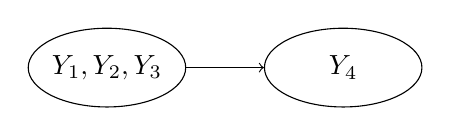
\begin{tikzpicture}
\node[draw,ellipse, minimum height=1cm, minimum width=2cm,inner sep=0pt] (00) at (0,0) {$Y_1, Y_2,Y_3$};
\node[draw,ellipse, minimum height=1cm, minimum width=2cm,inner sep=0pt] (10) at (3,0) {$Y_4$};
\draw[->] (00) -- (10);
\end{tikzpicture}
\hspace{2cm}
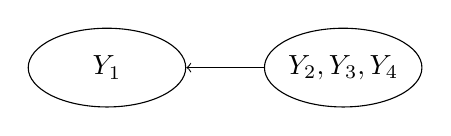
\begin{tikzpicture}
\node[draw,ellipse, minimum height=1cm, minimum width=2cm,inner sep=0pt] (00) at (0,0) {$Y_1$};
\node[draw,ellipse, minimum height=1cm, minimum width=2cm,inner sep=0pt] (10) at (3,0) {$Y_2,Y_3,Y_4$};
\draw[->] (10) -- (00);
\end{tikzpicture}
\end{center}
\caption{Possible conversions of the undirected graph in Figure \ref{fig:UG} into a directed acyclic graph.\label{fig:UGCG}}
\end{figure}

We note here however that there is situation in which updating can be distributed across panels using the original MN model that does not break the coherence of the IDSS (which recall does not respect variational independence). We formalise this case in the following theorem.

\begin{theorem}
\label{theo:UGIDSS}
Let $\Gr$ be an decomposable UG, $\mathcal{C}$ and $\mathcal{S}$ the sets of cliques and separators of $\Gr$ respectively, and assume panel $G_i$ oversees the variables in the clique $C_i\in\mathcal{C}$. Assume the IDSS is sound a priori and that each panel $G_i$ plans to update its beliefs using the dataset  $\bm{x}^t_i$, independent to the ones of other panels. Then the IDSS is also sound a posteriori iff $\bm{t}_i(\bm{x}^t_{i,S})$, the sufficient statistic for $\bm{\theta}_S$ of $\bm{x}^t_i$, is equal for every $S\in\mathcal{S}$ and for every $C_i\in\mathcal{C}$ such that $S\subset C_i$. 
\end{theorem}
The proof of this result is reported in Appendix \ref{proof:UGIDSS}.

Importantly this result shows that strong hyper Markov distributions are preserved when updated with incomplete datasets of a particular type - i.e. partial datasets covering together the whole graph and having consistent sufficient statistics over the separators.  

\begin{example}
Consider again the MN with graph in Figure \ref{fig:UG} and suppose a covariance selection model is defined over this network as shown in Section \ref{sec:UG}. Suppose two panels oversee the two cliques of this graph and assume that a strong hyper Markov distribution has been agreed over the graph. Suppose panels collect random samples from the same family of $\bm{Y}$ only over the variables they oversee, denoted as $\bm{x}^1=\big({\bm{x}_1^1}^\T,{\bm{x}_2^1}^\T,{\bm{x}_3^1}^\T\big)^\T$ for $G_1$ and $\bm{x}^2=\big({\bm{x}_2^2}^\T,{\bm{x}_3^2}^\T,{\bm{x}_4^2}^\T\big)^\T$ for $G_2$. Let a generic $\bm{x}_j^i=(x_{jk}^i)_{k\in[n_i]}^\T$. Then, as shown in equation (\ref{stica}), coherence is guaranteed a posteriori iff $\sum_{i\in [n_1]}(x_{2i}^1)^2=\sum_{i\in [n_2]}(x_{2i}^2)^2$, $\sum_{i\in [n_1]}(x_{3i}^1)^2=\sum_{i\in [n_2]}(x_{3i}^2)^2$ and $\sum_{i\in [n_1]}{x_{2i}^1}x_{3i}^1=\sum_{i\in [n_2]}x_{2i}^2x_{3i}^2$.
\end{example}

\subsubsection{Staged Trees and Chain Event Graphs.}
\label{sec:IDSSET}
 Suppose for each possible decision $\bm{d}\in\bm{\mathcal{D}}$, panels can agree the topology of the underlying event tree  $\mathcal{T}(\bm{d})$ and suppress the dependence on the decisions for ease of notation. Suppose also all agree that panel $G_{i}$, $i\in[m]$, should deliver the edge probability vectors $\bm{\theta }_{ij}$ associated with edges emanating from each non-leaf vertex $v_{ij}$, $j\in[m_i]$, $m_i\in\mathbb{Z}_{\geq 1}$. Let $\bm{\theta }_{ij}= ( \theta _{ijk})_{k\in [m_{ij}]}^\T$, for an $m_{ij}\in\mathbb{Z}_{\geq 1}$, $\bm{\theta }_{i}^\T= \big( \bm{\theta }_{ij}\big)_{j\in[m_i]}^\T$ and $\bm{\theta }^\T= \big( \bm{\theta }^\T_{i}\big)_{i\in[m]} $. Then, for example, under random sampling
\begin{align}
\label{nun}
l(\bm{\theta }\;|\;\bm{x})&=\prod_{i\in[m]}l_{i}(\bm{\theta }_{i}\;|\;\bm{x}),\\
\shortintertext{where} 
l_{i}(\bm{\theta }_{i}\;|\;\bm{x})&=\prod_{j\in[m_i]}l_{ij}(\bm{\theta }_{ij}\;|\;\bm{x}),\\
\shortintertext{and} 
l_{ij}(\bm{\theta }_{i}\;|\;\bm{x})&=\prod_{k\in[m_{ij}]}\theta _{ijk}^{x_{ijk}},
\label{ce}
\end{align}%
for $\sum_{k\in[m_{ij}]}\theta _{ijk}=1$ and $x_{ijk}$ is the number of units in the sample $\bm{x}$ reaching vertex $v_{ij}$ and then proceeding down the $k-${th} edge. Clearly this likelihood separates over the parameter vectors overseen by different panels. It can be similarly shown that this separability holds if the dataset $\bm{x}$ is ancestral - see \citet{Smith2010}. 

The conditions for distributivity in IDSSs whose structural consensus includes either a staged tree or a CEG are slightly stronger, but often met in practice. Let $\mathcal{T}$ be a staged tree now, with stage set $\mathbb{W}=\{w_i:i\in[n]\}$. Let $\bm{\theta}_{i}^{\mathbb{W}}$ be the probability vector associated to a stage $w_i$, $i\in[n]$. Unless $\bm{\theta}_i^{\mathbb{W}}=\bm{\theta}_{ij}$ for every $j\in[m_i]$ but one only $i\in[m]$, the distributed learning of equations (\ref{nun})-(\ref{ce}) breaks down, since different panels have jurisdiction over parameters that are identified (just as for OOBNs).  However, panels can be constituted in such a way that this condition is met. Note that distributivity also holds whenever panels oversee disjoint subsets of the position set (or equivalently disjoint subsets of the vertex set of a CEG), since the position set is a finer partition of the situations of a tree than the stage set.

 Thus CEGs and staged trees can provide a framework where data can be quickly accommodated in a distributed way (using the Dirichlet-Multinomial recursions discussed in Section \ref{sec:CEG}), given that the panels oversee either the positions or the stages of a CEG/staged tree. 

\begin{example}
Consider the staged tree in Figure \ref{fig:ET}. For distributivity to hold, a unique panel needs to have jurisdiction over the positions $v_3$ and $v_4$ since these are in the same stage.
\end{example}
\subsection{Dynamic Models}

The necessary separation conditions for IDSSs are not only entertained by non-dynamic models, as exemplified in Section \ref{sec:nondymidss} in a variety of domains, but also in situations where probabilities are allowed to be recursively updated in a dynamic fashion. For ease of notation, in this section we leave implicit the dependence on the decisions $\bm{d}$.

\subsubsection{Multiregression Dynamic Models.} 
The first model class we consider is the MDM. Since each time slice of an MDM conditionally on the past is described by a DAG, which does not change through time, the results concerning the use of BNs in IDSSs transfer to these dynamic models straightforwardly. 

We note that since a dynamic version of global independence is always assumed in MDMs (Proposition \ref{prop:MDM}), then panel independence is guaranteed whenever panels oversee disjoint subsets of the vertex set. Furthermore, the densities $f(\bm{y}_t\;|\;\bm{y}^{t-1})$ can be written as the product of functions overseen by individual panels. We formalise these concepts in the following proposition

\begin{proposition}
\label{prop:MDMIDSS}
Suppose the structural consensus of a CK-class includes an MDM model whose associated DAG has vertex set $\{\bm{Y}^T_i: i\in[n]\}$, where panel $G_i$ oversees the vector $\bm{Y}^T_{B_i}$, $i\in[m]$, where $B_1,\dots,B_m$ form a partition of $[n]$. It then follows that for every $t\in T$,
\begin{align}
\pi(\bm{\theta}(t)\;|\;I^{t-1})&=\prod_{i\in[m]}\pi_i(\bm{\theta}_{B_i}(t)\;|\;I^{t-1}),\label{uccidimi}\\
f(\bm{y}(t)\;|\;\bm{y}^{t-1})&=\prod_{i\in[m]}\int_{\bm{\Theta}_{B_i}}f_i(\bm{y}_{B_i}(t)\;|\;\bm{y}^t_{\Pi_{B_i}},\bm{y}_{B_i}^{t-1},\bm{\theta}_{B_i})\pi_i(\bm{\theta}_{B_i}(t)\;|\; I^{t-1})\dr\bm{\theta}_{B_i}(t).\label{tiprego}
\end{align}
\end{proposition} 
\begin{proof}
Equation (\ref{uccidimi}) is implied by the independence structure underlying MDMs specified in Proposition \ref{prop:MDM}. Equation (\ref{tiprego}) is an instance of equations (\ref{eq:mdmmarg}) and (\ref{eq:mdmeq2}) in Proposition \ref{prop:MDM2} applied to vectors of parameters overseen by different panels. 
\end{proof}


\begin{example}
Consider the MDM whose associated DAG is in Figure \ref{fig:MDM} and suppose  panels $G_1$ and $G_2 $ have jurisdiction over $(\bm{Y}_1^T,\bm{Y}^T_2)$ and $(\bm{Y}_3^T,\bm{Y}_4^T)$, respectively. Panel independence in this setting implies that, for any $t\in[T]$, $(\bm{\theta}_1(t),\bm{\theta}_2(t))\independent (\bm{\theta}_3(t),\bm{\theta}_4(t))\;|\;I^{t-1}$. Furthermore the marginal density of the observables, conditional on the past, can be written as
\begin{equation*}
f(\bm{y}(t)\;|\;I^{t-1})=f_2(y_3(t),y_{4}(t)\;|\;y_{2}(t),I^{t-1})f_1(y_1(t),y_2(t)\;|\;I^{t-1}),
\end{equation*}
where 
\begin{align*}
f_2(y_3(t),y_{4}(t)\;|\;y_{2}(t),I^{t-1})&=\int_{\bm{\Theta}_{34}}f_2(y_3(t),y_{4}(t)\;|\;y_{2}(t),I^{t-1},\bm{\theta}_{34})\pi_2(\bm{\theta}_{34}\;|\; I^{t-1})\dr \bm{\theta}_{34},\\
f_1(y_1(t),y_2(t)\;|\;I^{t-1})&=\int_{\bm{\Theta}_{12}}f_1(y_1(t),y_2(t)\;|\;I^{t-1},\bm{\theta}_{12})\pi_1(\bm{\theta}_{12}\;|\; I^{t-1})\dr \bm{\theta}_{12}.
\end{align*}
\end{example}

We are also able to show that the combination rules of \citet{Faria1997}, generalised to IDSSs in Proposition \ref{prop:combi}, can be extended to dynamic frameworks.
\begin{proposition}
\label{prop:dyncombi}
Under the conditions of Proposition \ref{prop:MDMIDSS}, assume the underlying DAG is decomposable and each panel agrees to aggregate the density of each member using a conditional logOp. Then the IDSS respects the CEB property if densities are backward sequentially updated through the vertices of the DAG and through time.
\end{proposition}

\begin{proof}
The proposition follows by Proposition \ref{prop:combi}, since each time slice of the MDM can be thought of, conditional on the past, as a BN, whose underlying DAG does not change through time.
\end{proof}


\subsubsection{Dynamic Chain Graphs.}
A generalisation of the class of MDM models is the DCG model class introduced in Section \ref{sec:DCG}. As discussed for PCG models, the CG associated to a DCGs can be converted into a DAG whose vertex set consists of the strong components of the initial CG. Therefore, as for PCGs and BNs, the conditions required for DCGs to be in the structural consensus of a coherent IDSS are the same as the ones of MDMs, but applied to the strong components of the associated CG.

\section{Conclusions}
 In this chapter we have introduced the IDSS framework to coherently aggregate the judgements of separate panels of experts agreeing on a common knowledge base. This extends standard Bayesian reasoning in single agent frameworks to ones where beliefs are delivered by many experts. We have shown in Theorem \ref{theo:gold} that the conditions for the existence of a coherent IDSS are not overly restrictive. By introducing a new notion of causality, we have then demonstrated that Bayesian learning can be distributed to the different panels of experts, guaranteeing fast inferential routines, just as in the standard Bayesian framework. We have then concluded the chapter showing that a suite of standard Bayesian graphical models can be part of the structural consensus of an IDSS. To do this, we have generalised standard independence notions and learning routines of these common graphical models.  
\input{Chapters/Chapter4} 
% Chapter Template

\chapter{The Algebra of Integrating Partial Belief Systems} % Main chapter title

\label{chapter5} % Change X to a consecutive number; for referencing this chapter elsewhere, use \ref{ChapterX}

\lhead{Chapter 5. \emph{The Algebra of Integrated Partial Belief Systems}} % Change X to a consecutive number; this is for the header on each page - perhaps a shortened title

%----------------------------------------------------------------------------------------
%	SECTION 1
%----------------------------------------------------------------------------------------

The examples of Section \ref{sec:exalgo} showed that the IDSS's expected utilities are often polynomial functions whose indeterminates are individually delivered by different panels. By requesting only this information, the implementation of an IDSS can become orders of magnitude more manageable. This is because panels just need to communicate a few summaries from their sample: a trivial and fast task to perform. 

Therefore, for the sole purpose of decision support, the full inferential conditions guaranteeing a sound and distributed analysis of Chapter \ref{chapter3} are actually too strict. These can be relaxed whilst retaining the coherence of the IDSS. Taking an algebraic approach, in this chapter we develop  a methodology that ensures coherence in these types of partially defined systems, meaning systems where panels only deliver certain selected summaries. Following \citet{Leonelli2015b}, we first define the new notion of algebraic expected utility of an IDSS. This definition enables us to impose new conditions tailored to the needs of an IDSS concerning the uncorrelatedness of certain polynomials. These conditions, often weaker than panel independence, can guarantee an IDSS is adequate. We discuss how and when it is possible to achieve adequacy in a number of typical frameworks. Importantly, this algebraic approach enables us to extend results about the computation of moments of decomposable functions in DAGs \citep{Cowell1999a, Nilsson2001} for a particular subclass of BN models.  

Although this is not often recognised in the literature, algebraic approaches are intimately linked to symbolic ones, where probabilities are treated as indeterminates in a computer algebra system, thus not requiring an exact numerical specification. Symbolic inference is often used in sensitivity analysis to identify the probabilities a DM needs to be particularly precise about in her specification, as these might drastically change the ranking of the available policies \citep{French2003}. We symbolically define two important instances of models that can be part of an IDSS structural consensus, namely IDs and staged trees. We develop new symbolic inferential techniques for these two models, extending  current literature to both decision and asymmetric problems. An extensive discussion of these results can be found in \citet{Leonelli2015a} and \citet{Gorgen2015}. 

 The structure of the chapter is as follows. In Section \ref{sec:history} we  review the main developments in symbolic and algebraic inferential methods. In Section \ref{sec:description} we  define algebraically the  expected utility of an  IDSS. Section \ref{sec:momind} introduces polynomial conditions the panels' summaries need to entertain and we then show in Section \ref{sec:adequacy1} how these are able to guarantee adequacy and distributivity. Section \ref{sec:parexamples} presents a variety of examples of these methods. In Section \ref{sec:short} we review recent symbolic methods for two particular integrating structures: IDs and staged trees. We conclude with a discussion.
 
\section{A Brief Overview of Symbolic and Algebraic Methods in Statistics}
\label{sec:history}
As mentioned in the introduction, symbolic and algebraic methods for statistical inference have been developed independently by two different community of researchers. Symbolic ones have been the focus of mostly computer scientists, whilst algebraic ones of mathematicians and statisticians. However, in both cases, the probabilities associated to a statistical model are described as polynomials, whose structure is then exploited to study the inferential properties of such models in a variety of applications. 

Symbolic methods focused mostly on graphical models and specifically on BNs, both discrete \citep{Castillo1995,Castillo1997a} and Gaussian \citep{Castillo1997}. Probabilities and moments associated to vertices are thought of as indeterminates of a computer algebra system (such as Maple or Matlab), where the model's probabilities can then be seen as polynomials with such indeterminates.  \citet{Castillo1996a} and \citet{Castillo2003} developed and implemented algorithms for the computation of polynomials associated to the joint probabilities of a BN model. In these works the bounds the probabilities of the vertices of the network have to respect were also identified, and these can then be used in sensitivity analyses. The fundamental idea behind this approach lies in the fact that once the qualitative structure of the model is constructed, numerical specifications of the involved probabilities do not need to be delivered a priori for the algorithms to run. Furthermore the above mentioned bounds inform a DM about probability values that cannot be delivered, thus simplifying the elicitation process. 

However, the symbolic inferential algorithms of \citet{Castillo1997b} had several drawbacks. Most importantly these computed \textit{every} possible monomial deriving from the symbolic definition of the model, only later dropping those associated to non compatible instantiations. This required the computation of the Cartesian product  of the sets of probabilities associated to the vertices of the BN, which can become infeasible as the size of the network grows. In \citet{Darwiche2003} a new symbolic inferential algorithm speeded up the computation of the probability polynomials, by converting the underlying BN into an \textit{Arithmetic Circuit (AC)}. This circuit can then be evaluated through fast routines to output the required polynomials. Importantly, \citet{Darwiche2003} also showed that a large number of probabilistic queries can be answered by computing certain \textit{derivatives} of the probability polynomials, which are then easier to handle because the associated AC has a smaller dimension. Such methods were subsequently extended to DBNs \citep{Brandherm2004}.

Beside the possibility of not having to elicit probabilities before any inference takes place, another great advantage of symbolic approaches is that these methods straightforwardly support various \textit{sensitivity analyses}. In particular users can simply plug-in different numbers into the probability indeterminates and observe how these change the inferential results on a set of goal variables. Alternatively, much more sophisticated sensitivity techniques have now been implemented \citep{Chan2001,Chan2004}. 

Although the computing capability of modern computers is constantly growing, it has been possible to apply symbolic approaches only in small/medium sized applications. This is because each probability specification is treated as an unknown variable in a computer system. This requires much more memory space than a single number. Furthermore, as shown by \citet{Cooper1990}, the number of monomials in BN models grows exponentially with the number of vertices, often making the computation of such polynomials prohibitive. However, we note here that the technology of IDSSs allows us to apply symbolic methods to much larger models. This is because we can define symbolically only the \textit{outputs} of each component DSS, which is the only relevant information an IDSS needs to process. At the same time, this symbolic definition leads straightforwardly to the use of sensitivity analyses for the outputs of IDSSs, which can be extremely useful for building consensus among the panel members. 

The alternative stream of research using polynomial techniques in statistics is usually referred to as \textit{algebraic statistics}. Among others, this uses techniques from algebraic geometry and computational commutative algebra to gain insights into the structure of certain statistical models \citep{Riccomagno2009a}. The first developments of algebraic statistics were on  the use of both Gr\"{o}bner bases in Markov chain sampling algorithms \citep{Diaconis1998} and commutative algebraic techniques in the design and analysis of experiments \citep{Pistone1996}. 

Subsequently, algebraic statistics also started to be applied to more general statistical models. Certain statistical models have been identified with certain algebraic varieties \citep{Pistone2002}. Big part of the research in this area then focused on graphical models, as for example BNs \citep{Garcia2005, Sullivant2008}, MNs \citep{Geiger2006} and trees \citep{Settimi2000}. The number of applications of algebraic methods in statistics is now enormous \citep[see e.g. the monographs,][]{Gibilisco2010, Pistone2002, Drton2009b, Pachter2005}.

To our knowledge, the methods we develop in the following sections are the first application of symbolic and algebraic techniques to Bayesian decision analysis.  

\section{An Algebraic Description of Integrating Systems}
\label{sec:description}
The computation of the expected utilities in the examples of Section \ref{sec:exalgo} showed the difficulty of identifying the beliefs that need to be delivered  to the IDSS by panels. The situation becomes even more complicated when the utility consensus includes multilinear or multiplicative utility factorisations introduced in Definitions \ref{def:multilinear} and \ref{def:multiplicative} respectively (unless all panels can simply define independent marginal models for the variables under their jurisdiction). 

Approaching the problem from an algebraic viewpoint allows us to identify the necessary panels' summaries and the required assumptions for adequacy. In order to do this we first need to define the expected utility polynomials. Recall that there are $m $ panels of experts $\{G_i:i\in[m]\}$, $[m]=\{1,\dots,m\}$, each delivering beliefs about $\bm{\theta}_i$, $i\in[m]$, parametrising the density of $\bm{Y}_i\;|\;\bm{d}$, for a decision $\bm{d}\in\bm{\mathcal{D}}$. The conditional expected utility is $\bar{u}(\bm{d}\;|\;\bm{\theta})$, whilst $\bar{u}(\bm{d})$ is the expected utility.

\begin{definition}
The conditional expected utility $\bar{u}(\bm{d}\;|\;\bm{\theta})$ of an IDSS is called \textbf{algebraic} if, for each $\bm{d}\in \bm{\mathcal{D}}$ and $\bm{\theta} \in \bm{\Theta} $, $\bar{u}(\bm{d}\;|\;\bm{\theta})$ is a square-free polynomial 
\[
\bar{u}(\bm{d}\;|\;\bm{\theta})=f_{\bm{d}}\left( \bm{\lambda}_{1}(\bm{\theta}_{1},\bm{d}),\cdots,\bm{\lambda}_m(\bm{\theta }_{m},\bm{d})\right) 
\]
 in functions $\bm{\lambda }_{_{i}}(\bm{\theta }_{i},\bm{d})$ of the parameters $\bm{\theta }_{_{i}}$ of panel $G_{i}$, $i\in[m]$.
\end{definition}

We now explicitly define the algebraic conditional expected utilities $f_{\bm{d}} $. Let $\bm{\lambda}_i(\bm{\theta}_i,\bm{d})=(\lambda _{ji}(\bm{\theta }_{i},\bm{d}))^\T_{j\in[s_i]}$, for an $s_i\in\mathbb{Z}_{\geq 1}$, and $\bm{b}\in B=\bigtimes_{i\in[m]}B_{i}$ , where $B_{i}=[s_i]^0=[s_i]\cup \{0\}$, $i\in[m]$. For a given $\bm{b}$, let $i\in B_j$ be its j-th entry and let $b(j,i)=0$ if $j\neq i$, $b(j,i)=1$ if $j=i$ and $b(0,i)=1$, for $i\in[m]$ and $j\in[s_i]$. Then, if we define $\lambda_{0i}(\bm{\theta}_i,\bm{d})=1$, for every $\bm{\theta}_i\in \bm{\Theta}_i$, $\bm{d}\in\bm{\mathcal{D}}$ and $i\in[m]$, we can write 
\begin{equation}
f_{\bm{d}}\left( \bm{\lambda }_{_{1}}(\bm{\theta }_{1},\bm{d}),\dots,\bm{\lambda }_{m}(\bm{\theta }_{m},\bm{d})\right)  = \sum_{\bm{b}\in B}k_{\bm{b},\bm{d}}\lambda _{\bm{b}}(\bm{ \theta },\bm{d}),  \label{algebraic utility} \end{equation}
where
\begin{equation*}
 \lambda _{\bm{b}}(\bm{\theta },\bm{d}) = \prod_{i\in[m]}\prod_{j\in[s_i]^0}\lambda_{ji}(\bm{\theta }_{i},\bm{d})^{b(j,i)},  \label{eq:aceu2}
\end{equation*}
is a monomial, having at most one term not unity delivered by each panel. So in particular, $f_{\bm{d}} $ is a square-free polynomial. For a given $\bm{b}\in B$, let
\begin{equation*}
\mu _{ji}(\bm{d})= \mathbb{E}\left( \lambda_{ji}(\bm{\theta }_{i},\bm{d})^{b(j,i)}\right). 
\end{equation*}

For the distributivity of the IDSS we need the following property.
\begin{definition}
Call an IDSS \textbf{score separable} if, in the notation above, the collective agrees that, for all decisions $\bm{d}\in \bm{\mathcal{D}}$ and all indices $\bm{b}\in B$ such that $k_{\bm{b},\bm{d}}\neq 0$,
\begin{equation}
\mathbb{E}\left( \lambda _{\bm{b}}(\bm{\theta },\bm{d})\right)=\prod_{i\in[m]}\prod_{j\in[s_i]^0}\mu_{ji}(\bm{d}). \label{uncor}
\end{equation}
\label{def:scoresep}
\end{definition}
 Let, for every $\bm{d}\in\bm{\mathcal{D}}$, $\bm{\mu }_{i}(\bm{d})=\left( \mu _{ji}(\bm{d})\right)^\T_{j\in[s_i]}$. A consequence of the definitions above is the following. 

\begin{lemma}
\label{lemma:ciao}
Suppose panel $G_{i}$ delivers its vectors of expectations $\bm{\mu }_{i}(\bm{d})$, $i\in[m]$, $\bm{d}\in\bm{\mathcal{D}}$, to the SB. Then, under the collective assumptions of an algebraic conditional expected utility, if the IDSS is score separable then it is  adequate.
\end{lemma}
\begin{proof}
The definition of adequacy in Definition \ref{def:adequacy} means in this framework that the expected utility $\bar{u}(\bm{d})$ is a function of $\mu_{ji}(\bm{d})$ and $k_{\bm{b},\bm{d}}$ only, for $i\in[m]$, $j\in[s_i]^0$, $\bm{b}\in B$ and $\bm{d}\in\bm{\mathcal{D}}$.  Now note that 
\begin{equation*}
\bar{u}(\bm{d})=\E\left(f_{\bm{d}}\left( \bm{\lambda }_{_{1}}(\bm{\theta }_{1},\bm{d}),\dots,\bm{\lambda }_{m}(\bm{\theta }_{m},\bm{d})\right)\right)= \sum_{\bm{b}\in B}k_{\bm{b},\bm{d}}\E\left(\lambda _{\bm{b}}(\bm{ \theta },\bm{d})\right).\label{eq:nonso}
\end{equation*}
The definition of score separability in equation (\ref{uncor}) then implies that 
\begin{equation*}
\bar{u}(\bm{d})=\sum_{\bm{b}\in B}k_{\bm{b},\bm{d}} \prod_{i\in[m]}\prod_{j\in[s_i]^0}\mu_{ji}(\bm{d}),
\end{equation*}
from which the lemma follows.
\end{proof}

 We can therefore deduce from Lemma \ref{lemma:ciao} that adequacy is guaranteed whenever score separability holds, under the assumption of an algebraic conditional expected utility. In the following section we introduce conditions that ensure this type of separability. We then identify classes of models that give rise to algebraic conditional expected utilities.

\section{Moment and Partial Independence}
\label{sec:momind}
Equation (\ref{uncor}) together with Lemma \ref{lemma:ciao} shows that adequacy is guaranteed whenever the expectation of certain functions of the panels' parameters separate appropriately. We introduce now a new type of independence called \textit{partial independence}.
\begin{definition}
\label{def:partial}
Let $f_{\bm{d}}(\bm{\lambda }_{_{1}}(\bm{\theta }_{1},\bm{d}),\dots,\bm{\lambda }_{m}(\bm{\theta }_{m},\bm{d}))$ be the algebraic conditional expected utility of an IDSS. We say that an IDSS is \textbf{partially independent} if 
\begin{equation*}
\E(f_{\bm{d}}(\bm{\lambda }_{_{1}}(\bm{\theta }_{1},\bm{d}),\dots,\bm{\lambda }_{m}(\bm{\theta }_{m},\bm{d})))=f_{\bm{d}}(\E(\bm{\lambda }_{_{1}}(\bm{\theta }_{1},\bm{d})),\dots,\E(\bm{\lambda }_{m}(\bm{\theta }_{m},\bm{d}))).
\end{equation*}
\end{definition}
This condition requires the expectation of the product of certain functions of the parameters overseen by different panels to be equal to the product of the individual expectations.

Often the $\lambda_{ji}$, $i\in[m]$, $j\in[s_i]$, are monomial functions of the panels' parameters. It is therefore helpful to introduce the following independence condition specific for monomial functions. Let $<_{lex}$ denote a lexicographic order (see Appendix \ref{appendixC}).

\begin{definition}
\label{def:moment}
Let $\bm{\theta}=(\theta_i)^\T_{i\in[n]}\in\mathbb{R}^{n}$ be a parameter vector and $\bm{b}=(b_i)^\T_{i\in[n]}\in\mathbb{Z}^n_{\geq 0}$. We say that $\bm{\theta}$ entertains \textbf{moment independence} of order $\bm{b}$ if,  $\forall~\bm{b}'=\left(b_i'\right)_{i\in[n]}^\T\leq_{lex} \bm{b}$, 
\begin{equation*}
\E\left(\bm{\theta}^{\bm{b}'}\right)=\prod_{i\in[n]}\E\left(\theta_i^{b_i'}\right).
\end{equation*}
\end{definition}

It is generally well known that standard probabilistic independence only guarantees that the \textit{first} moment of a product can be written as the product of the moments. Separations for higher orders are implied by standard independence only through a cumulant parametrisation, where the cumulant generating function for a product of independent random variables (defined as a random sum of independent realisations) is the composition of the respective cumulant generating functions.

For the purpose of decision support in partial belief systems it is helpful to study moments, since expected utilities often formally depend on these. Consider for instance two parameters $\theta_1$ and $\theta_2$. Suppose a conditional expected utility is equal to $\theta_1^2\theta_2^2$ and that a moment independence of order $(2,2)$ holds. Then,
\begin{equation}
\mathbb{E}\left(\theta_1^2\theta_2^2\right)=\mathbb{E}\left(\theta_1^2\right)\mathbb{E}\left(\theta_2^2\right)=\mathbb{E}(\theta_1)^2\mathbb{E}(\theta_2)^2+\mathbb{E}(\theta_1)^2\mathbb{V}(\theta_2)+\mathbb{E}(\theta_2)^2\mathbb{V}(\theta_1)+\mathbb{V}(\theta_1)\mathbb{V}(\theta_2).
\label{eq:towerex}
\end{equation}
The same expression is obtained when using sequentially the tower rule of expectations and the law of total variance of Proposition \ref{prop:towerrules} under the assumption of independence of the two parameters above. Therefore, the expression obtained under moment independence is reasonable and coincides with the one implied by the independence of $\theta_1$ and $\theta_2$. However the condition we need for equation (\ref{eq:towerex}) to hold \textit{does not require} $\theta_1$ and $\theta_2$ to be independent. 

\section{Adequacy in Partially Defined Systems}
\label{sec:adequacy1}

 Given the definitions of new independence concepts tailored for IDSSs, we can now study in which cases adequacy holds. The following result easily follows from the definition of partial independence.
 
\begin{lemma}
\label{lemma:ciaociao}
Suppose $f_{\bm{d}}(\bm{\lambda }_{_{1}}(\bm{\theta }_{1},\bm{d}),\dots,\bm{\lambda }_{m}(\bm{\theta }_{m},\bm{d}))$ is the algebraic conditional expected utility of an IDSS and that partial independence is in the structural consensus. The IDSS is then adequate if panel $G_i$ delivers the expectations $\bm{u}_i(\bm{d})$, $i\in[m]$, $\bm{d}\in\bm{\mathcal{D}}$.
\end{lemma}
\begin{proof}
This result easily follows by noting that partial independence implies score separability. Specifically,
\begin{eqnarray*}
\bar{u}(\bm{d})&=&\E\left(f_{\bm{d}}(\bm{\lambda }_{_{1}}(\bm{\theta }_{1},\bm{d}),\dots,\bm{\lambda }_{m}(\bm{\theta }_{m},\bm{d}))\right)=f_{\bm{d}}(\E(\bm{\lambda }_{_{1}}(\bm{\theta }_{1},\bm{d})),\dots,\E(\bm{\lambda }_{m}(\bm{\theta }_{m},\bm{d})))\\
&=&\sum_{\bm{b}\in B}k_{\bm{b},\bm{d}} \prod_{i\in[m]}\prod_{j\in[s_i]^0}\mu_{ji}(\bm{d}).
\end{eqnarray*}
The result then follows from Lemma \ref{lemma:ciao}.
\end{proof}

Assuming the conditional expected utility is a polynomial in the panels' parameters, then under a specific moment independence assumption we have the following. 

\begin{lemma}
\label{lemma:ciao3}
Assume $f_{\bm{d}}(\bm{\lambda }_{_{1}}(\bm{\theta }_{1},\bm{d}),\dots,\bm{\lambda }_{m}(\bm{\theta }_{m},\bm{d}))$ is the algebraic conditional expected utility of an IDSS, $\bm{\theta}_i=(\theta_{ji})^\T_{j\in[s_i]}$ and $\lambda_{ji}(\bm{\theta}_i,\bm{d})=\bm{\theta}_{i}^{\bm{a}_{ji}}$, with $\bm{a}_{ji}\in\mathbb{Z}_{\geq 0}^{s_i}$, $i\in[m]$, $j\in[s_i]$. Let $\bm{a}^*_i=({a_{ji}^*})_{j\in[s_i]}^\T$, where $a_{ji}^*$ is the greatest element in $\{a_{ji}:j\in[s_i]\}$, $i\in[m]$, and let ${\bm{a}^*}^\T=({\bm{a}_i^*}^\T)_{i\in[m]}$. Let $\bm{\theta}=(\bm{\theta}_i^\T)_{i\in[m]}^\T$ and assume the structural consensus includes the assumption that $\bm{\theta}$ entertains moment independence of order $\bm{a}^*$. Then the IDSS is adequate if panel $G_i$ delivers  the vectors of expectations $\bm{u}_i(\bm{d})$, $i\in[m]$, $\bm{d}\in\bm{\mathcal{D}}$.
\end{lemma} 
\begin{proof}
Adequacy is again guaranteed if the expected utility function can be written in terms of $\mu_{ji}(\bm{d})$, $i\in[m]$, $j\in[s_i]$ and $\bm{d}\in\bm{\mathcal{D}}$. Note that
\begin{eqnarray*}
\bar{u}(\bm{d})&=&\E\left(f_{\bm{d}}(\bm{\lambda }_{_{1}}(\bm{\theta }_{1},\bm{d}),\dots,\bm{\lambda }_{m}(\bm{\theta }_{m},\bm{d}))\right)=\sum_{\bm{b}\in B}k_{\bm{b},\bm{d}}\E\left( \prod_{i\in[m]}\prod_{j\in[s_i]^0}\lambda_{ji}(\bm{\theta }_{i},\bm{d})^{b(j,i)}\right)\\
&=&\sum_{\bm{b}\in B}k_{\bm{b},\bm{d}}\E\left(\prod_{i\in[m]}\prod_{j\in[s_i]^0}\bm{\theta}_i^{\bm{a}_{ji}}\right).
\end{eqnarray*}
The argument of this expectation is then a monomial of multi-degree lower or equal to $\bm{a}^*$ with respect to a lexicographic order. Moment independence then implies that 
\begin{equation*}
\bar{u}(\bm{d})=\sum_{\bm{b}\in B}k_{\bm{b},\bm{d}}\prod_{i\in[m]}\prod_{j\in[s_i]^0}\mu_{ji}(\bm{d}),
\end{equation*}
and the result follows.
\end{proof}

Both Lemma \ref{lemma:ciaociao} and \ref{lemma:ciao3} start with the assumption of an algebraic conditional expected utility. This is the case for many of the examples we consider in Section \ref{sec:parexamples}. However, we are able to identify families of utility factorisations and statistical models that ensure the associated conditional expected utility is algebraic.  We first introduce two families of utilities that factorise according to the construction of the panels.
\begin{definition}
\label{def:panelsep}
Let $\bm{Y}_i$ be the vector overseen by panel $G_i$, $i\in[m]$, and $\bm{R}_i$ be a function of $\bm{Y}_i$ and $\bm{d}\in\bm{\mathcal{D}}$ only. A multilinear factorisation over $\bm{R}_1,\dots,\bm{R}_m$ is called \textbf{panel separable}.   
\end{definition}

\begin{definition}
Under the conditions of Definition \ref{def:panelsep}, an additive factorisation over $\bm{R}_1,\dots, \bm{R}_m$ is called \emph{additive panel separable}.
\end{definition}

Both families of panel separable and additive panel separable utilities can be seen as a particular instance of a compatible utility factorisation in Definition \ref{compatible}. 

The probabilistic model class we consider here is a generalisation of the DAG linear regressions in equation (\ref{eq:GausBN}) to generic polynomial functions. Henceforth we call these a \textit{polynomial Structural Equation Model (SEM)} \citep[see e.g.][]{Bollen1998,Ullman2003,Wall2000}. SEMs are widely used, especially recently, in the causal literature \citep{Pearl2000}. 

\begin{definition}
\label{def:polystrut}
Let $\bm{Y}=(Y_i)^\T_{i\in[n]}$ be a random vector. A \textbf{polynomial SEM} is defined by, for $i\in[n]$,
\begin{equation*}
Y_i=\sum_{\bm{b}_i\in B_i}\theta_{i\bm{b}_i}\bm{Y}_{[i-1]}^{\bm{b}_i}+\varepsilon_i,
\end{equation*}
where $B_i\subset \mathbb{Z}^{i-1}_{\geq 0}$, $\varepsilon_i$ is an error with mean zero and variance $\psi$, and $\theta_{i\bm{b}_i}$ is a parameter, $i\in[n]$, $\bm{b}_i\in B_i$.
\end{definition}

An alternative formulation of the model in Definition \ref{def:polystrut} in terms of distributions is,  
\begin{equation*}
Y_i\;|\;\bm{\theta}_i,\bm{Y}_{[i-1]}\sim \Big(\sum_{\bm{b}_i\in B_i}\theta_{i\bm{b}_i}\bm{Y}_{[i-1]}^{\bm{b}_i},\psi_i\Big),
\end{equation*}
where $\bm{\theta}_i=(\psi_i,\theta_{i\bm{b}_i})^\T_{\bm{b}_i\in B_i}$ and $i\in[n]$.

Note that these models are suitable candidates for a CK-class since their definition is qualitative in nature.
 
For polynomial SEMs and panel separable utilities, the following holds.
\begin{theorem}
\label{theo:ciao}
Suppose $\bm{R}=\bm{Y}$ and assume panel $G_i$ is responsible for $Y_i$, $i\in[n]$. Assume that the utility consensus of an IDSS includes a panel separable utility and that the structural consensus includes a polynomial SEM. Suppose each panel agreed to model its marginal utility as a polynomial utility function. Then if panels are partially independent, the IDSS is score separable.
\end{theorem}

The proof of this result can be found in Appendix \ref{proof:theociao}.

Theorem \ref{theo:ciao} together with Lemma \ref{lemma:ciao} can be thought of as an instance of the important Theorem \ref{theo:gold}, specifically addressing adequacy in partial belief systems. An IDSS whose CK-class embeds the assumptions of Theorem \ref{theo:ciao} is able to uniquely compute expected utility scores from the individual judgements of the panels. 

Note that, by construction, the partial independence condition of Theorem \ref{theo:ciao} actually corresponds  to a moment independence. The order of such an independence depends on the polynomial form of both the SEM and the utility function. In Section \ref{sec:bn1} we  identify the order of the moment independence condition required for adequacy for a subclass of polynomial SEMs.

\section{Examples}
\label{sec:parexamples}
\subsection{Discrete Models}
\subsubsection{Independence Binary Models.}
We begin with a rather obvious setting where a small number of summaries are sufficient to determine an expected utility maximising decision. Let the CK-class specify that $\bm{R}=\bm{Y}=(Y_i)_{i\in[n]}^\T$, where each variable $Y_i$ is binary and overseen by panel $G_i$. Assume the CK-class includes the belief that $\independent_{i\in[n]} Y_i\;|\; \bm{\theta},\bm{d}$, where $\bm{\theta}=(\theta_i)_{i\in[n]}^\T$ and that $\theta_i$ can be read as the probability $\mathbb{P}(Y_i=1\;|\;\theta_i,\bm{d})$, whatever decision $\bm{d}\in\bm{\mathcal{D}}$ is made, $i\in[n]$. We have already discussed in Section \ref{sec:indadd} how independence models can be part of the structural consensus of a CK-class. 

As in the example in Section \ref{sec:adequacy}, suppose each panel $G_i$ delivers the set of beta distributions $\Be(p_i,q_i)$ for $\theta_i\;|\;\bm{d}$, $i\in[n]$.  Assume further the CK-class includes utility factorisations of the form
\begin{equation*}
\label{eq:ind1}
u(y_1,\dots, y_n)=\sum_{i\in[n]}k_iy_i+\sum_{i\in[n]}\sum_{j\in[n]_i}k_{ij}y_iy_j.
\end{equation*}
With no further assumptions, the conditional expected utility can be written as
\begin{equation}
\label{eq:ind2}
\bar{u}(\bm{d}\;|\;\bm{\theta})=\sum_{i\in[n]}k_i\lambda_i(\theta_i,\bm{d})+\sum_{i\in[n]}\sum_{j\in[n]_i}k_{ij}\lambda_i(\theta_i,\bm{d})\lambda_j(\theta_j,\bm{d}),
\end{equation}
where $\lambda_i(\theta_i,\bm{d})=\theta_i$, $[n]_i=\{i+1,\dots,n\}$. Thus,  equation (\ref{eq:ind2}) is an algebraic conditional expected utility. In this example  partial independence then corresponds to moment independence of order $\bm{1}$, where $\bm{1}$ is a vector of dimension $n$ with $1$ in all its entries. In this case, partial independence is implied by panel independence. Furthermore all the monomials $\lambda_{\bm{b}}(\bm{\theta},d)$ formally defined in equation (\ref{algebraic utility}) here are monomials of degree  either  one or two corresponding respectively to $\lambda_i(\theta_i,\bm{d})$ or $\lambda_i(\theta_i,\bm{d})\lambda_j(\theta_j,\bm{d})$, for $i\in[n]$ and $j\in[n]_i$.

Now let $\mu_i=p_i(p_i+q_i)^{-1}=\mathbb{E}(\theta_i\;|\;\bm{d})$ and assume partial independence is in the CK-class. We can see that taking the expectation of equation (\ref{eq:ind2}) we have that
\begin{equation*}
\label{eq:ind3}
\bar{u}(\bm{d})=\sum_{i\in[n]}k_i\mu_i+\sum_{i\in[n]}\sum_{j\in[n]_i}k_{ij}\mu_i\mu_j,
\end{equation*}
where $\bar{u}(d)$ is the expected utility. Thus this IDSS is adequate. Note that this IDSS does not need panel independence to uniquely compute expected utility scores, but only a simple moment independence. 


\subsubsection{Staged Trees.}
Consider now the staged tree in Figure \ref{fig:ET} of Section \ref{sec:tree}, that we report again on page \pageref{riporto} for convenience. As discussed in Section \ref{sec:IDSSET}, staged trees can be part of a coherent IDSS whenever panels oversee disjoint subsets of either the position set or the stage set. Recall that this tree has four stages (coinciding with its positions) $w_0=\{v_0\},$ $w_1=\{v_1\}$, $w_2=\{v_2\}$ and $w_3=\{v_3,v_4\}$. Suppose there are three panels $G_1$, $G_2$ and $G_3$ having responsibility over $w_0$, $\{w_1,w_2\}$ and $w_3$ respectively.

\begin{figure}
\centerline{
\hspace*{-16mm} \xymatrixrowsep{0.5pc}{\xymatrixcolsep{2pc}
\xymatrix{
&&&&\bullet~v_{7}\\
&&&\bullet~v_{3}\ar@[red][r]_{\text{no}}\ar@[blue][ru]^{\text{yes}}&\bullet~v_{8}\\
&&\bullet~v_{1}\ar[r]_{\text{low}}\ar[ru]^{\text{high}}&\bullet~v_{4}\ar@[blue][r]|{\text{yes}}\ar@[red][rd]_{\text{no}}&\bullet~v_{9}\\
v_0\hspace*{-16mm}&\bullet\ar[ru]^{\text{yes}}\ar[rd]_{\text{no}}&&&\bullet~v_{10}\\
&&\bullet~v_{2}\ar[r]^{\text{high}}\ar[rd]_{\text{low}}&\bullet~v_{5}\\
&&&\bullet~v_{6}
}}}
\label{riporto}
\end{figure}

In the notation of Example \ref{ex:staged}, assume the collective has agreed on an additive utility factorisation such that 
\[
u(y_1,y_2,y_3)=k_1u_1(y_1)+k_2u_2(y_2)+k_3u_3(y_3),
\]
where $Y_1,Y_2,Y_3$ are the variables in the associated BN representation of this tree, and that they have been jointly able to further specify the criterion weights.  Label the outcomes of this tree with a $1$ for yes and high, whilst a $0$ denotes no and low outcomes. Let $\psi_{ij}=u_i(j)$, where $j\in\{0,1\}$, and recall that $\theta_{ss'}=\mathbb{P}(Y_s=s'\;|\;\bm{\theta},\bm{d})$, for a situation $s\in S(\mathcal{T})$, $s'\in\mathcal{Y}_s=\{1,0\}$ and $\bm{d}\in\bm{\mathcal{D}}$, where $\bm{\theta}$ is the overall parameter vector. In this parametrisation, the staged tree in Figure \ref{fig:ET} introduces the constraints $\theta_{31}=\theta_{41}$ and $\theta_{30}=\theta_{40}$, where for example $\theta_{31}=\mathbb{P}(Y_3=\text{yes}\;|\; Y_2=\text{high}, Y_1=\text{yes},\bm{\theta},\bm{d})$.

Through a sequential application of the tower rule of expectation, it can be easily deduced that the conditional expected utility of this problem can be written as
\begin{equation}
\label{eq:staged2}
\bar{u}(\bm{\theta}\;|\;\bm{d})=\bar{u}_1+\bar{u}_2+\bar{u}_{3},
\end{equation}
where
\begin{align}
\begin{split}
\label{eq:staged3}
&\bar{u}_1=k_1\psi_{11}\theta_{01}+k_1\psi_{10}\theta_{00},\\
&\bar{u}_2=k_2\psi_{21}\theta_{11}\theta_{01}+k_2\psi_{20}\theta_{10}\theta_{01}+k_2\psi_{21}\theta_{21}\theta_{00}+k_2\psi_{20}\theta_{20}\theta_{00},\\
&\bar{u}_{3}=k_3\psi_{31}\theta_{31}\theta_{11}\theta_{01}+k_3\psi_{30}\theta_{30}\theta_{11}\theta_{01}+k_3\psi_{31}\theta_{41}\theta_{10}\theta_{01}+k_3\psi_{30}\theta_{40}\theta_{10}\theta_{01}.
\end{split}
\end{align}

So the conditional expected utility in equations (\ref{eq:staged2})-(\ref{eq:staged3}) is again algebraic. The coefficients $k_{\bm{b},\bm{d}}$ of the monomials in equation (\ref{algebraic utility}) correspond to the jointly agreed criterion weights, and the unknown functions $\bm{\lambda}_{i}(\bm{\theta}_i,\bm{d})$ are as follows 
\begin{align*}
\bm{\lambda}_1(\bm{\theta}_1,\bm{d})&=(\psi_{11}\theta_{01},\psi_{10}\theta_{00})^\T,\\
\bm{\lambda}_2(\bm{\theta}_2,\bm{d})&=(\theta_{11},\theta_{10},\theta_{21},\theta_{20},\psi_{21}\theta_{11},\psi_{20}\theta_{10},\psi_{21}\theta_{21},\psi_{20}\theta_{20})^\T,\\
\bm{\lambda}_3(\bm{\theta}_3,\bm{d})&=(\psi_{31}\theta_{31},\psi_{30}\theta_{30})^\T.
\end{align*}
Thus once more these polynomials are a simple multilinear function of probabilities delivered by different panels. Under partial independence, as guaranteed by  Lemma \ref{lemma:ciao}, an IDSS so defined is adequate. 
 
\subsection{Bayesian Networks}
\label{sec:bn1}

We now consider the BN model class, where each variable of the network is defined as the DAG linear regression introduced in  Definition \ref{def:linreg}. Note that this is an instance of the polynomial SEM of Definition \ref{def:polystrut}. We refer to this model as a \textit{linear SEM} over a DAG $\Gr$.  Although such a model is often multivariate Gaussian, in general this does not have to be the case.

Just as \citet{Sullivant2008}, we consider regression parameters as indeterminates in a polynomial function. We associate these to edges and vertices of the underlying DAG. Let $\Gr$ be a DAG with vertex set $V(\Gr)=\{Y_i:i\in[n]\}$ and let, for $i\in[n]$, $\theta_{0i}'=\theta_{0i}+\varepsilon_{i}$ be the indeterminate associated to the vertex $Y_i$, whilst $\theta_{ij}$, for $(Y_i,Y_j)\in E(\Gr)$, is the indeterminate associated to the corresponding edge.\footnote{We think of $\theta_{0i}'$ as a parameter although this consists of the sum of a parameter and an error. Note however that from a Bayesian viewpoint these are  both random variables.} Define $\vec{P}_i$ as the set of rooted directed paths (see Appendix \ref{appendixB}) in $\Gr$ ending in $Y_i$. For every element $P\in\vec{P}_i$ we define $\bm{\theta}_P$ as
 \begin{equation*}
 \bm{\theta}_P=\prod_{Y_i\in P}\theta_{0i}'\prod_{(Y_i,Y_j)\in P}\theta_{ij},
 \end{equation*}
and we call $\bm{\theta}_{P}$ the \textit{path monomial}.

\begin{example}
Consider the DAG in Figure \ref{fig:BNexample}. The set $\vec{P}_3$ for instance is equal to
\begin{equation}
\label{eq:paths}
\{(Y_3),(Y_2,(Y_2,Y_3)), (Y_1,(Y_1,Y_3)), (Y_1,(Y_1,Y_2),(Y_2,Y_3))\},
\end{equation}
and $\theta_{03}'$, $\theta_{02}'\theta_{23}$, $\theta_{01}'\theta_{13}$ and $\theta_{01}'\theta_{12}\theta_{23}$ are the corresponding path monomials.
\end{example}

For the purpose of this section we call \textit{algebraic substitution} the process of plugging-in the linear regression definition of a random variable of the DAG into the structural equation definition of the child variable. To illustrate this process, we present now an example of what we mean by an algebraic substitution. 

\begin{example}
Consider again the DAG in Figure \ref{fig:BNexample}. For this network the variables are defined as
\begin{equation*}
\begin{array}{lccl}
Y_4=\theta_{04}+\theta_{14}Y_1+\varepsilon_1, &&& Y_3=\theta_{03}+\theta_{13}Y_1+\theta_{23}Y_2+\varepsilon_3,\\
Y_2=\theta_{02}+\theta_{12}Y_1+\varepsilon_2,&&& Y_1=\theta_{01}+\varepsilon_1.
\end{array}
\end{equation*}
An algebraic substitution of the variables in the definition of $Y_3$ entails
\begin{align}
Y_3&=\theta_{03}+\theta_{13}(\theta_{01}+\varepsilon_1)+\theta_{23}(\theta_{02}+\theta_{12}Y_1+\varepsilon_2)+\varepsilon_3\nonumber\\
&=\theta_{03'}+\theta_{13}\theta_{01}'+\theta_{23}\theta_{02}'+\theta_{23}\theta_{12}Y_1.\label{eq:y3}
\end{align}
Note that an additional algebraic substitution can be performed in equation (\ref{eq:y3}) so that 
\begin{equation}
Y_3=\theta_{03}'+\theta_{13}\theta_{01}'+\theta_{23}\theta_{02}'+\theta_{23}\theta_{12}\theta_{01}'.\label{eq:y3'}
\end{equation}
\end{example}
It is of special interest that after this substitution $Y_3$ is now uniquely defined in equation (\ref{eq:y3'}) in terms of regression parameters. The following proposition formalises that this is in general the case for any variable of a DAG defined as a linear SEM.

\begin{proposition}
\label{prop:algsub}
Let $\Gr$ be a DAG with vertex set $\{Y_i:i\in[n]\}$, whose variables are defined as a linear SEM. Then through algebraic substitutions each variable $Y_i$, $i\in[n]$, can be written as
\begin{equation*}
Y_i=\sum_{P\in\vec{P}_i}\bm{\theta}_{P}.
\end{equation*}
\end{proposition}
\begin{proof}
We prove this result via induction over the indices of the variables. The variable $Y_1$ is by construction a root of the DAG $\Gr$. Thus $Y_1=\theta_{01}'$, where $\theta_{01}'$ is the monomial associated to the only rooted path ending in $Y_1$, namely $(Y_1)$. Assume the result is true for $Y_{n-1}$ and consider $Y_{n}$. By construction and by the inductive hypothesis we have that  
\begin{equation}
Y_{n}=\theta_{0n}'+\sum_{i\in \Pi_n}\theta_{in}Y_i=\theta_{0n}'+\sum_{i\in \Pi_n}\theta_{in}\sum_{P\in \vec{P}_i}\bm{\theta}_P.
\label{eq:pathid}
\end{equation}
Note that every rooted path ending in $Y_n$ is either $(Y_n)$ or consists of a rooted path ending in $Y_i$, $i\in \Pi_n$, together with the edge $(Y_i,Y_n)$. From this observation the result then follows by rearranging the terms in equation (\ref{eq:pathid}).
\end{proof}
\begin{example}
Equation (\ref{eq:y3'}) shows that $Y_3$ can be written as the sum of the monomials associated to each rooted path ending in $Y_3$, where the set of rooted paths is in equation (\ref{eq:paths}).
\end{example}

An algebraic substitution corresponds to computing the conditional expectation of a random variable. This result is formalised by the following proposition.

\begin{proposition}
\label{prop:condex}
Let $\bm{\theta}^\T=(\bm{\theta}_i^\T)$, where $\bm{\theta}_{i}=(\theta_{0i}',\theta_{ji})_{j\in \Pi_i}^\T$, $i\in[n]$. Under the conditions of Proposition \ref{prop:algsub}, we have that 
\[
\E(Y_i\;|\;\bm{\theta},\bm{d})=\sum_{P\in\vec{P}_i}\bm{\theta}_P.
\]
\begin{proof}
This result is proven via the same inductive process as in the proof of Proposition \ref{prop:algsub}. Note that the result holds for $Y_1$ since $\E(Y_1\;|\;\bm{\theta})=\theta_{01}'$. Assume the proposition is true for $Y_{n-1}$ and consider $Y_n$. We have that 
\begin{eqnarray*}
\E(Y_n\;|\;\bm{\theta},\bm{d})&=&\E(\E(Y_n\;|\;\bm{\theta}_n,\bm{Y}_{\Pi_n},\bm{d})\;|\;\bm{\theta},\bm{d})=\E\Big(\theta_{0n}'+\sum_{i\in[n]}\theta_{in}Y_i\;|\;\bm{\theta},\bm{d}\Big)\\
&=&\theta_{0n}'+\sum_{i\in[n]}\theta_{in}\E(Y_i\;|\;\bm{\theta},\bm{d})=\theta_{0n}'+\sum_{i\in[n]}\theta_{in}\sum_{P\in\vec{P}_i}\bm{\theta}_P.
\end{eqnarray*}
Using a similar argument as in the proof of Proposition \ref{prop:algsub} the result follows.
\end{proof}
\end{proposition}
\subsubsection{Additive Factorisations.}
Given Propositions \ref{prop:algsub} and \ref{prop:condex}, we are now able to polynomially compute the expected utility of additive utility factorisations over the graphs in the case the marginal utility functions are polynomial.

\begin{lemma}
\label{lemma:addeu}
For a linear SEM over a DAG $\Gr$ with vertex set $\{Y_i:i\in[n]\}$, suppose $\bm{R}=\bm{Y}$ and that the utility function $u(\bm{r})$ can be written
\begin{equation*}
u(\bm{r})=\sum_{i\in[n]}k_iu_i(y_i).
\end{equation*}
Suppose further $u_i$ is a polynomial utility function of degree $n_i$, i.e. $u_i=\sum_{j\in[n_i]}\rho_{ij}y_i^j$. Then the conditional expected utility is algebraic and can be written as
\begin{equation}
\label{eq:addeu}
\bar{u}(\bm{d}\;|\;\bm{\theta})=\sum_{i\in[n]}k_i\sum_{j\in[n_i]^0}\rho_{ij}\sum_{|\bm{\alpha}_i|=j}\binom{j}{\bm{\alpha}_i}\bm{\theta}_{\Gr_i}^{\bm{\alpha}_i},
\end{equation}
where $\bm{\alpha}_i=(\alpha_{ij})^\T_{j\in[\#\vec{P}_i]}\in\mathbb{Z}_{\geq 0}^{\#\vec{P}_i}$, $\#\vec{P}_i$ is the number of elements in $\vec{P}_i$, $|\bm{\alpha}_i|=\sum_{j\in[\#\vec{P}_i]}\alpha_{ij}$, $\bm{\theta}_{\Gr_i}=\prod_{P\in\vec{P}_i}\bm{\theta}_P$ and $\binom{j}{\bm{\alpha}_i}$ is a Multinomial coefficient (see Appendix \ref{sec:multidir}).
\end{lemma}

\begin{proof}
From Proposition \ref{prop:condex}, it follows that
\begin{equation*}
\label{eq:additiveEU}
\E(u(\bm{R})\;|\;\bm{\theta},\bm{d})=\sum_{i\in[n]}k_i\sum_{j\in[n_i]^0}\rho_{ij}\bigg(\sum_{P\in\vec{P}_i}\bm{\theta}_P\bigg)^j.
\end{equation*}
The result follows applying the Multinomial theorem (see Appendix \ref{appendixC}).
\end{proof}

Equation (\ref{eq:addeu}) is an instance of the computation of the moments of a decomposable function as studied in \citet{Cowell1999a} and \citet{Nilsson2001}, where in this case we explicitly deduce the required monomials and their degree. In the following section we generalise their results to generic multilinear functions. 

The proof of Lemma \ref{lemma:addeu} provides an intuitive graphical description of the required monomials for the computation of the expected utility in equation (\ref{eq:addeu}). Furthermore the proof instructs us on how to compute any marginal moment of a linear SEM. Note that the $j$-th moment of any variable $Y_i$ in such a BN can be written, via the Multinomial theorem, as the sum of the monomials $\bm{\theta}_{\Gr_i}$ with degree $j$. We can observe that, following from the properties of Multinomial coefficients, this sum can be thought of as the sum over the set of unordered $j$-tuples of paths ending in $Y_i$. Call this set $\vec{P}^j_i$. For a $j$-tuple $P\in\vec{P}^j_i$, the Multinomial coefficient in equation (\ref{eq:addeu}) counts the distinct permutations of the elements of $P$, denoted as $n_P$. We therefore have that
\begin{equation}
\label{eq:grapheu}
\sum_{|\bm{\alpha}_i|=j}\binom{j}{\bm{\alpha}_i}\bm{\theta}_{\Gr_i}^{\bm{\alpha}_i}=\sum_{P\in\vec{P}^j_i}n_P\prod_{p\in P}\bm{\theta}_p.
\end{equation} 
 Equation (\ref{eq:grapheu}) is an intuitive graphical interpretation of equation (\ref{eq:addeu}).

\begin{example}
For simplicity we consider now the vertex $Y_4$ in the DAG of Figure \ref{fig:BNexample}. The set $\vec{P}_4$ is equal to $\{(Y_4), (Y_1,(Y_1,Y_4))\}$. From equation (\ref{eq:addeu}), $Y_4^2$ can be written as 
\begin{equation}
\label{eq:exbn1}
\theta'^2_{04}+\theta'^2_{01}\theta_{14}^2+2\theta_{01}'\theta_{14}\theta_{04}'.
\end{equation}
The polynomial above can be equally deduced by simply looking at the DAG. Note that 
\begin{equation*}
\vec{P}_4^2=\Big\{\big((Y_4),(Y_4)\big), \big((Y_1,(Y_1,Y_4)),(Y_1,(Y_1,Y_4))\big), \big((Y_4),(Y_1,(Y_1,Y_4))\big)\Big\}.
\end{equation*}
The first and second monomial in equation (\ref{eq:exbn1}) correspond to the first and second element of $\vec{P}_4^2$ respectively, whilst the last elements of this set, having two distinct permutation of its elements, is associated to the third monomial in equation (\ref{eq:exbn1})
\end{example}

From Lemma \ref{lemma:addeu} we can deduce the independence needed for adequacy in BNs. 
\begin{theorem}
\label{theo:pr}
Suppose $\bm{R}=\bm{Y} $ and that the structural consensus of an IDSS includes a linear SEM over a DAG with vertex set $\{Y_i:i\in[n]\}$, where panel $G_i$ oversees the vertex $Y_i$ of $\Gr$, $i\in[n]$. Suppose the utility consensus consists of an additive panel separable utility function and panel $G_i$ agreed to model its marginal utility with a polynomial utility function of degree $n_i\in\mathbb{Z}_{\geq 1}$, $i\in[n]$. Let $l_P$ be the length of a rooted path $P$, $l_i=\sum_{P\in\vec{P}_i}l_P$ and $\bm{\alpha}_i\in\mathbb{Z}^{l_i}_{\geq 0}$. If $\bm{\theta}_{\Gr_i}$ entertains moment independence of order $\bm{\alpha}_i$ for every $|\bm{\alpha}_i|=n_i$ and $i\in[n]$, then the IDSS is score separable.  
\end{theorem}
\begin{proof}
Under the assumptions of the theorem, the conditional expected utility function can be written as in equation (\ref{eq:addeu}). From the linearity of the expectation operator we have that
\[
\bar{u}(\bm{d})=\E(\bar{u}(\bm{d}\;|\;\bm{\theta}))= \sum_{i\in[n]}k_i\sum_{j\in[n_i]^0}\rho_{ij}\sum_{|\bm{\alpha}_i|=j}\binom{j}{\bm{\alpha}_i}\E\left(\bm{\theta}_{\Gr_i}^{\bm{\alpha}_i}\;|\;\bm{d}\right).
\]
Noting that $\bm{\theta}_{\Gr_i}=\prod_{P\in\vec{P}_i}\bm{\theta}_P$, $\bm{\theta}_P=\prod_{Y_i\in P}\theta_{0i}'\prod_{(Y_j,Y_k)\in P}\theta_{jk}$ and applying moment independence, we have that  
\[
\bar{u}(\bm{d})= \sum_{\substack{i\in[n], j\in[n_i]^0,\\ |\bm{\alpha}_i|=j}}k_i\rho_{ij}\binom{j}{\bm{\alpha}_i}\prod_{P\in\vec{P}_i,Y_l\in P}\E\left(\theta_{0l}'^{\alpha_{il}}\theta_{lCh_l}^{\alpha_{lCh_l}}\;|\;\bm{d}\right)\hspace{-0.2cm}\prod_{(Y_j,Y_k)\in P\setminus (Y_l,Y_{Ch_l})}\hspace{-0.2cm}\E\left(\theta_{jk}^{\alpha_{ik}}\;|\;\bm{d}\right),
\]
where $\alpha_{ij}$ is the element of $\bm{\alpha}_i$ associated to $\theta_{kj}$. The lemma  then follows since $\bar{u}(\bm{d})$ is a multilinear function of expectations individually delivered by the panels.
\end{proof}

Theorem \ref{theo:pr} can be seen as an instance of Theorem \ref{theo:ciao} where we have been able to identify the specific moment independences necessary for the IDSS's adequacy. By requesting the collective to agree on these independences, the IDSS can then quickly produce a unique expected utility score for each policy. Furthermore, panels are informed about the summaries that they need to deliver to the IDSS since these are the only quantities the expected utility is a function of. 

We can observe that in this case the functions $\lambda_{ij}$ panel $G_i$ delivers, $i\in[n]$, $j\in[s_i]$, are simply powers of monomials having one or two indeterminates only. Therefore, if panels deliver the expectation of these functions, where the required degrees are specified by Theorem \ref{theo:pr}, an IDSS so defined will be adequate. 

\subsubsection{Multilinear Factorisations.}
The algebraic approach we have taken in this chapter allows us to generalise  straightforwardly the results on additive/decomposable functions to multilinear functions. We start analysing this more general case by stating two introductory results. 

\begin{proposition}
\label{prop:1}
Let $\Gr$ be a DAG with vertex set $\{Y_i:i\in[n]\}$ and assume $\bm{R}=\bm{Y}$. Assume a multilinear utility factorisation over the graph such that
\begin{equation*}
\label{eq:multidag}
u(\bm{r})=\sum_{I\in\mathcal{P}_0([n])}k_I\prod_{i\in I}u_i(y_i),
\end{equation*} 
where $\mathcal{P}_0$ denotes the power set without the empty set. Then letting each marginal utility $u_i(y_i)$ be polynomial of degree $n_i$ and $\bm{n}=(n_i)_{i\in[n]}^\T\in\mathbb{Z}^n$,
\begin{equation}
\label{eq:multiutpol}
u(\bm{r})=\sum_{\bm{0}<_{lex}\bm{\alpha}\leq_{lex}\bm{n}}c_{\bm{\alpha}}\bm{y}^{\bm{\alpha}},
\end{equation}
where $\bm{\alpha}=(\alpha_i)_{i\in[n]}^\T\in\mathbb{Z}^{n}_{\geq 0}$, $c_{\bm{\alpha}}=k_J\prod_{j\in J}\rho_{j\alpha_j}$ and $J=\{j\in[n]: \alpha_j\neq 0\}$. 
\end{proposition}

The proof of this result is given in Appendix \ref{proof:basta}.

\begin{proposition}
\label{prop:2}
For a linear SEM over $\Gr$ with vertex set $\{Y_i:i\in[n]\}$, letting $\bm{\alpha}=(\alpha_i)_{i\in[n]}^\T\in\mathbb{Z}^{n}_{\geq 0}$ and assuming $\#\vec{P}_i=n_i$, $i\in[n]$, we have that 
\begin{equation}
\label{eq:multiciao}
\bm{Y}^{\bm{\alpha}}=\sum_{\bm{\beta}\simeq \bm{\alpha}}\binom{|\bm{\alpha}|}{\bm{\beta}}\bm{\theta}_{\Gr}^{\bm{\beta}},
\end{equation}
where $\bm{\beta}=(\bm{\beta}_i^\T)^\T_{i\in[n]}$, $\bm{\beta}_i=(\beta_{ij})^\T_{j\in[n_i]}\in\mathbb{Z}^{n_i}_{\geq 0}$, $\bm{\theta}_{\Gr}=\prod_{i\in[n]}\bm{\theta}_{\Gr_i}$ and we write $\bm{\alpha}\simeq \bm{\beta}$ if both $|\bm{\alpha}|=|\bm{\beta}|$ and $\forall ~ i\in[n]$ , $|\bm{\beta}_i|=\alpha_i$.  
\end{proposition}

\begin{proof} The monomial $\bm{Y}^{\bm{\alpha}}$ can be written as
\begin{align*}
\bm{Y}^{\bm{\alpha}}&=\prod_{i\in[n]}Y_i^{\alpha_i}=\prod_{i\in[n]}\left(\sum_{|\bm{\beta}_i|=\alpha_i}\binom{\alpha_i}{\bm{\beta}_i}\bm{\theta}_{\Gr_i}^{\bm{\beta}_i}\right)=\sum_{\bm{\beta}\simeq \bm{\alpha}}\bm{\theta}_{\Gr}^{\bm{\beta}}\prod_{i\in[n]}\binom{\alpha_i}{\bm{\beta_i}}.
\end{align*}
Noting that 
\begin{equation*}
\prod_{i\in[n]}\binom{\alpha_i}{\bm{\beta}_i}=\frac{\prod_{i\in[n]}\alpha_i!}{\prod_{i\in[n]}\prod_{j\in[n_i]}\beta_{ij}!}=\binom{|\bm{\alpha}|}{\bm{\beta}},
\end{equation*}
the result follows.
\end{proof}

From the previous two results we then deduce the following.
\begin{lemma}
\label{lemma:multieu}
Under the assumptions of Propositions \ref{prop:1} and \ref{prop:2}, the conditional expected utility is algebraic and can be written as
\begin{equation}
\label{eq:multieu}
\bar{u}(\bm{d}\;|\;\bm{\theta})=\sum_{\bm{0}<_{lex}\bm{\alpha}\leq_{lex}\bm{n}}c_{\bm{\alpha}}\sum_{\bm{\beta}\simeq \bm{\alpha}}\binom{|\bm{\alpha}|}{\bm{\beta}}\bm{\theta}_{\Gr}^{\bm{\beta}}.
\end{equation}
\end{lemma}

\begin{proof}
This follows by plugging in equation (\ref{eq:multiciao}) into equation (\ref{eq:multiutpol}).
\end{proof}

Although straightforward, Lemma \ref{lemma:multieu} makes a significant generalisation to the theory of the computation of moments in decomposable/additive functions of \citet{Cowell1999a} and \citet{Nilsson2001} to multilinear functions of BNs defined as a linear SEM. This result is also connected to the propagation algorithms first developed in \citet{Lauritzen1992}. In that paper, the computation of the first two moments of a much larger class of models (chain graphs with both discrete and continuous variables) is considered. Here, focusing only on a certain class of continuous DAG models, we are able to explicitly compute, through algebraic substitution, any moment of the distribution associated to the graph.  

Using again the properties of Multinomial coefficients, we can relate  equation (\ref{eq:multieu}) to the topology of the graph and its rooted paths. For an $\bm{\alpha}\in\mathbb{Z}^{n}_{\geq 0}$, let $\vec{P}^{\bm{\alpha}}$ be the set of unordered $|\bm{\alpha}|$-tuples of paths, where in each tuple there are $\alpha_i$ paths ending in $Y_i$. For each element $P\in\vec{P}^{\bm{\alpha}}$, let $n_P$ be the sum of $n_{P_i}$, the number of distinct permutations of  paths ending in $Y_i$ in $\vec{P}^{\bm{\alpha}}$. Then we have that
 \begin{equation*}
 \sum_{\bm{\beta}\simeq \bm{\alpha}}\binom{|\bm{\alpha}|}{\bm{\beta}}\bm{\theta}_{\Gr}^{\bm{\beta}}=\sum_{P\in\vec{P}^{\bm{\alpha}}}n_P\prod_{p\in P}\bm{\theta}_p.
 \end{equation*}
 \begin{example}
 Consider $\E(Y_2^2Y_4^2)$. All distinct tuples of dimension four where two paths end in $Y_2$ and two  in $Y_4$ are summarised in Table \ref{table:tuples}. The associated conditional expectation can be written as the following polynomials, where the $i$-th monomial corresponds to the tuple in the $i$-th row of Table $\ref{table:tuples}$:
 \begin{multline*}
 \bar{u}(\bm{d}\;|\;\bm{\theta})=\theta'^2_{02}\theta'^2_{04}+
 2\theta_{12}{\theta_{02}'}\theta'^2_{04}+
 \theta_{12}^2\theta'^2_{04}+
 2\theta'^2_{02}\theta_{14}\theta_{04}'+
\\ 4\theta_{12}\theta_{02}'\theta_{14}\theta_{04}+
 2\theta_{12}^2\theta_{14}\theta_{04}'+
 \theta'^2_{02}\theta_{14}^2+
 2\theta_{12}\theta_{02}'\theta_{14}^2+
 \theta_{12}^2\theta_{14}^2.
 \end{multline*}
 Note for example that $\theta_{12}{\theta_{02}'}\theta'^2_{04}$ has coefficient 2 since the paths $(Y_2)$ and $(Y_1,(Y_1,Y_2))$ can be permuted, whilst $\theta_{12}\theta_{02}'\theta_{14}\theta_{04}$ has coefficient 4 since both pairs of paths $(Y_2)$ and $(Y_1,(Y_1,Y_2))$ and $(Y_4)$ and $(Y_1,(Y_1,Y_4))$ can be permuted.
 \end{example}
 
 \begin{table}
 \renewcommand{\arraystretch}{1.5}
 \begin{center}
 \begin{tabular}{|c|}
 \hline
 $((Y_2),(Y_2),(Y_4),(Y_4))$\\
 $((Y_1,(Y_1,Y_2)),(Y_2),(Y_4),(Y_4))$\\
 $((Y_1,(Y_1,Y_2)),(Y_1,(Y_1,Y_2)),(Y_4),(Y_4))$\\
 $((Y_2),(Y_2),(Y_1,(Y_1,Y_4)),(Y_4))$\\
 $((Y_1,(Y_1,Y_2)),(Y_2),(Y_1,(Y_1,Y_4)),(Y_4))$\\
  $((Y_1,(Y_1,Y_2)),(Y_1,(Y_1,Y_2)),(Y_1,(Y_1,Y_4)),(Y_4))$\\
  $((Y_2),(Y_2),(Y_1,(Y_1,Y_4)),(Y_1,(Y_1,Y_4)))$\\
 $((Y_1,(Y_1,Y_2)),(Y_2),(Y_1,(Y_1,Y_4)),(Y_1,(Y_1,Y_4)))$\\
 $((Y_1,(Y_1,Y_2)),(Y_1,(Y_1,Y_2)),(Y_1,(Y_1,Y_4)),(Y_1,(Y_1,Y_4)))$\\
 \hline
 \end{tabular}
 \end{center}
 \caption{Tuples of dimension 4 with two paths ending in $Y_2$ and two ending in $Y_4$ in the graph of Figure \ref{fig:BNexample}. \label{table:tuples}}
 \end{table}

Just as in the additive case, we are now able to deduce the independences required for score separability of an IDSS defined over a BN.

\begin{theorem}
Suppose $\bm{R}=\bm{Y}$ and that the structural consensus of an IDSS includes a linear SEM over a DAG with vertex set $\{Y_i:i\in[n]\}$, where panel $G_i$ oversees the vertex $Y_i$ of $\Gr$, $i\in[n]$. Suppose the utility consensus consists of a panel separable  utility and panel $G_i$ agreed to model its marginal utility with a polynomial utility function of degree $n_i\in\mathbb{Z}_{>0}$, $i\in[n]$. Let $l_i=\#\vec{P}_i$ and $l_{\Gr}=\sum_{i\in[n]}l_i$, $i\in[n]$. Let $\bm{\alpha}_{\Gr}=(\bm{\alpha}_i^\T)^\T_{i\in[n]}\in\mathbb{Z}^{l_\Gr}_{\geq 0}$, $\bm{\alpha}_i=(\alpha_{iP})^\T_{P\in\vec{P}_i}$ and $\bm{n}=(n_i)_{i\in[n]}^\T\in\mathbb{Z}^{n}_{\geq 0}$. If, for every $\bm{\alpha}\simeq \bm{n}$  $\bm{\theta}_{\Gr}=(\bm{\theta}_i)_{i\in[n]}^\T$, with $\bm{\theta}_i=(\bm{\theta}_{P})^\T_{P\in\vec{P}_i}$, entertains moment independence of order $\bm{\alpha}$, then the IDSS is score separable.  
\end{theorem}
 \begin{proof}
Under the conditions of the theorem, the conditional expected utility function can be written as in (\ref{eq:multieu}). The linearity of the expectation operator than implies that
\[
\E(\bar{u}(\bm{d}\;|\;\bm{\theta}))=\sum_{\bm{0}<_{lex}\bm{\alpha}\leq_{lex}\bm{n}}c_{\bm{\alpha}}\sum_{\bm{\beta}\simeq \bm{\alpha}}\binom{|\bm{\alpha}|}{\bm{\beta}}\E\left(\bm{\theta}_{\Gr}^{\bm{\alpha}}\;|\;\bm{d}\right).
\]
Now note that 
\[
\bm{\theta}_{\Gr}=\prod_{i\in[n]}\bm{\theta}_{\Gr_i}=\prod_{i\in[n]}\prod_{P\in\vec{P}_i}\bm{\theta}_P=\prod_{i\in[n]}\prod_{P\in\vec{P}_i}\prod_{Y_l\in P}\theta_{0l}'\prod_{(Y_j,Y_k)\in P}\theta_{jk}.
\]
Taking the expectation of $\bm{\theta}_{\Gr}^{\bm{\alpha}}$ we then have that 
\begin{eqnarray*}
\E\left(\bm{\theta}_{\Gr}^{\bm{\alpha}}\;|\;\bm{d}\right)&=& \E\bigg(\prod_{i\in[n]}\bm{\theta}_{\Gr_i}^{\bm{\alpha}_i}\;|\;\bm{d}\bigg)=\E\bigg(\prod_{i\in[n]}\prod_{P\in\vec{P}_i}\bm{\theta}_{P}^{\alpha_{iP}}\;|\;\bm{d}\bigg)\\
&=&\E\bigg(\prod_{i\in[n]}\prod_{P\in\vec{P}_i}\prod_{Y_l\in P}\theta_{0l}'^{\alpha_{iP}}\prod_{(Y_j,Y_k)\in P}\theta_{jk}^{\alpha_{iP}}\;|\;\bm{d}\bigg),\\
&=&\prod_{i\in[n]}\prod_{P\in\vec{P}_i}\prod_{Y_l\in P}\E\left((\theta_{0l}'\theta_{lCh_l})^{\alpha_{iP}}\;|\;\bm{d}\right)\prod_{(Y_j,Y_k)\in P \setminus (Y_l,Y_{Ch_l})}\E\left(\theta_{jk}^{\alpha_{iP}}\;|\;\bm{d}\right),
\end{eqnarray*}
where the last equality follows from moment independence. Score separability then follows.
 \end{proof}
 
This theorem generalises Theorem \ref{theo:pr} to multilinear utility factorisations and thus to a much larger class of IDSSs. 

  
\subsection{Conflict Models}
In this section we exploit the algebraic structure of the conditional expected utility of some simple IDSSs to deduce which panels' belief specification leads to either agreement or disagreement between the members of the collective. 
 
\subsubsection{A First Simple Example.}
\label{sec:quadratic}
Suppose an IDSS simply consists of two random variables, $Y_1$ and $Y_2$, assumed independent of each other and overseen by two different panels. For instance $Y_1$ might represent the costs deriving from a nuclear accident, whilst $Y_2$ is the number of people not exposed by the contamination. Suppose  the optimal number  $d\in \mathbb{Z}_{0< d\leq D}$, $D\in\mathbb{Z}$, of inhabitants to be evacuated from a nearby village needs to be found. Assume $Y_i\;|\;\theta_i,d\sim \Exp(\theta_i/d)$, $\theta_i\in\mathbb{R}_{> 0}$, $i\in[2]$, so that $Y_i$ follows an exponential distribution with density $\theta_ie^{-\theta_iy_i}$,  and let
\begin{equation*}
u(y_1,y_2)=k_1u_1(y_1)+k_2u_2(y_2),
\end{equation*}
with $u_1(y_1)=-\alpha_1y_1^2-\beta_1y_1+\gamma_1$, $u_2(y_2)=\alpha_2y_2^2+\beta_2y_2$ and $\alpha_1,\alpha_2,\beta_1,\beta_2,\gamma_1\in\mathbb{R}_{\geq 0}$. Recall that $\E(Y_i\;|\;d,\theta_i)=d/\theta_i$ and $\V(Y_i\;|\;\theta_i,d)=d^2/\theta_i^2$. Then as the number of people evacuated increases, both the costs and the number of non exposed people increase as well. Furthermore note that $u_1$ and $u_2$ are respectively an increasing and decreasing function of their arguments in $\mathbb{R}_{\geq 0}$.

It can be easily deduced that the conditional expected utility for an IDSS so defined is  equal to
\begin{eqnarray*}
\bar{u}(d\;|\;\bm{\theta})=\E(u(Y_1,Y_2)\;|\;\bm{\theta},\bm{d})&=&k_1\left(-2\frac{\alpha_1d^2}{\theta_1^2}-\frac{\beta_1d}{\theta_1}+\gamma_1\right)+k_2\left(2\frac{\alpha_2d^2}{\theta_2^2}+\frac{\beta_2d}{\theta_2}\right)\\
&=&2\left(\frac{k_2\alpha_2}{\theta_2^2}-\frac{k_1\alpha_1}{\theta_1^2}\right)d^2+\left(\frac{k_2\beta_2}{\theta_2}-\frac{k_1\beta_1}{\theta_1}\right)d+k_1\gamma_1.
\end{eqnarray*}   
This is a quadratic function of the decision $d$. Note that if 
\begin{equation*}
\frac{k_2\alpha_2}{\theta_2^2}>\frac{k_1\alpha_1}{\theta_1^2},
\end{equation*}
then $\bar{u}(d\;|\;\bm{\theta})$ is concave. Assuming $k_2\beta_2/\theta_2<k_1\beta_1/\theta_1$, otherwise the maximum of the function tends to zero, $\bar{u}(d\;|\;\bm{\theta})$ is maximal for some point $d^*$ within the interval $(0,D]$. Therefore optimal policies will in general consist of a balancing of the two attributes and both panels are likely to agree on such a course of action. 

On the other hand when 
\begin{equation*}
\frac{k_2\alpha_2}{\theta_2^2}<\frac{k_1\alpha_1}{\theta_1^2},
\end{equation*}
then $\bar{u}(d\;|\;\bm{\theta})$ is convex. In this case then the maximum will either be at $D$ or approaching zero,  corresponding to only optimising the cost or the exposition attributes respectively. In this situation it will be difficult for panels to agree on the outputs of the IDSS and any policy choice might be contentious. Note that when the coefficient of $d^2$ is close to zero, then small changes in the elicitation of the parameters might lead to a change from one of the two cases described above to the other. 
  
\subsubsection{A More Composite Scenario.}
Although the previous example shed light on the information that the conditional expected utility function carries about the behaviour of its optimal, the study of this behaviour was based on simple analytic concepts. We now consider a more difficult situation and use results from catastrophe theory \citep{Poston2014,Zeeman1979} in the context of expected utility maximisation similarly to \citet{Dodd2012} and \citet{Smith2012}.

Suppose an IDSS is defined as in Section \ref{sec:quadratic} above, with the only difference that the utility consensus now includes the utility factorisation
\begin{equation*}
u(y_1,y_2)=u_1(y_1)u_2(y_2).
\end{equation*}  
The conditional expected utility can then be computed as
\begin{eqnarray*}
\bar{u}(d\;|\;\bm{\theta})&=& \left(-2\frac{\alpha_1d^2}{\theta_1^2}-\frac{\beta_1d}{\theta_1}+\gamma_1\right)\left(2\frac{\alpha_2d^2}{\theta_2^2}+\frac{\beta_2d}{\theta_2}\right) \\
&=&-4\frac{\alpha_1\alpha_2}{\theta_1^2\theta_2^2}d^4-2\left(\frac{\alpha_1\beta_2\theta_2+\beta_1\alpha_2\theta_1}{\theta_1^2\theta_2^2}\right)d^3+\frac{2\gamma_1\alpha_2\theta_1^2-\beta_1\beta_2\theta_1\theta_2}{\theta_2^2\theta_1^2}d^2+\frac{\gamma_1\beta_2}{\theta_2}d.
\end{eqnarray*}

In order to study the behaviour of the maxima of this function we first differentiate this expansion and then equate it to zero. Specifically,
\begin{equation*}
\frac{\dr}{\dr d}\bar{u}(d)=d^3+\frac{2}{3}\frac{\alpha_2b_1+b_2\alpha_1}{a}d^2+\frac{b_2b_1-2\alpha_2c}{2a}d-\frac{b_2c}{4a},
\end{equation*}
where $a=\alpha_1\alpha_2$, $b_1=\beta_1\lambda_1$, $b_2=\beta_2\lambda_2$ and $c=\lambda_1^2\gamma_1$. By letting $e=\frac{2}{3}\frac{\alpha_2b_1+b_2\alpha_1}{a}$, $f=\frac{b_2b_1-2\alpha_2c}{2a}$, $g=-\frac{b_2c}{4a}$ and $z=d+\frac{e}{3}$, the equation above can be set to zero as
\begin{equation*}
z^3+\left(f-\frac{1}{3}e^2\right)z +\left(g+2\left(\frac{e}{3}\right)^3-\frac{ef}{3}\right)=0.
\end{equation*}
The local maxima of the conditional expected utility can therefore be described, as in \citet{Smith2012}, by the canonical cusp catastrophe \citep{Zeeman1979}, where the splitting factor of this cusp catastrophe is $-(f-(1/3)e^2)$. Therefore when 
\begin{equation*}
f-\frac{1}{3}e^2\geq 0 \;\;\;\;\; \Longleftrightarrow \;\;\;\;\; \alpha_1\left(\frac{19}{54}b_2b_1\alpha_2-b_2^2\alpha_1\right)\geq \alpha_2^2\left(c\alpha_1+\frac{4}{27}b_1^2\right),
\end{equation*}
the conditional expected utility has one local maximum only: a compromise between the two attributes. 

On the other hand if $f-\frac{1}{3}e^2< 0$, then for values of $g+2\left(\frac{e}{3}\right)^3-\frac{ef}{3}$ close to zero, the maximum of the expected utility function will either tend to $d=0$ or be $d=D$. In this case the optimal decision will only aim at minimising either the costs or the number of people exposed. In such a situations small changes of the parameters might then lead to opposite optimal decision rules and agreement within the collective might be difficult to reach. 

\section{A Note on Some New Symbolic Methods}
\label{sec:short}
This section reports recent developments on symbolic methods for inference and decision making in both MIDs and staged trees from \citet{Leonelli2015a} and \citet{Gorgen2015}, respectively. Although these results will not be discussed within the IDSS framework, we saw in Section \ref{sec:idssex} that both these model classes can be included in the structural consensus of a coherent and distributed IDSS under certain conditions. Therefore the results below can enhance the support an IDSS provides in practice. 
 
\subsection{Symbolic Evaluation of Influence Diagrams}
\label{sec:symbolic}
In this section we introduce a symbolic definition of MIDs and develop a symbolic evaluation algorithm. The implementation of this algorithm with our Maple code is reported in Appendix \ref{appendixD}. 

Let $\Gr$ be a Multiplicative Influence Diagram (MID) in extensive form with vertex set $\{Y_i, u_j:j\in[m], i\in[n]\}$. Assume each variable $Y_i$, $i\in[n]$, takes values in $\mathcal{Y}_i=[r_{i-1}]^0$.

\subsubsection{Polynomial Structure of Expected Utilities.}
\begin{figure}
\vspace{0.8cm}
\centerline{
\xymatrix{
*+[F]{Y_1}\ar@/^2pc/[rr]\ar[r]\ar[rd]&*+[Fo]{Y_3}\ar[dl]\ar@/^2pc/[rr]\ar[r]&*+[F]{Y_4}\ar[d]\ar[r]\ar[rd]&*+[Fo]{Y_5}\ar[r]\ar[d]&u_2\\
u_1&*+[Fo]{Y_2}\ar[u]\ar[ru]&u_3&*+[Fo]{Y_6}\ar[l]&
}
}
\vspace{0.2cm}
\label{fig:riporto}
\end{figure}
Generalising the work in \citet{Darwiche2003} and \citet{Castillo1995}, we introduce a symbolic representation of both the probabilities and the utilities of an  MID. For $i\in \mathbb{V}$, $j\in[m]$, and any $y\in\mathcal{Y}_i$, $\pi\in\bm{\mathcal{Y}}_{\Pi_i}$ and  $\sigma\in \bm{\mathcal{Y}}_{P_j}$, we define the parameters
\[
\begin{array}{cccc}
p_{iy\pi}=\mathbb{P}(Y_i =y\; |\; \bm{Y}_{\Pi_i}=\pi), &&& \psi_{j\sigma}=u_j(\sigma).
\end{array}
\]
The first index of $p_{iy\pi}$ and $\psi_{j\sigma}$ refers to the random variable and the utility vertex respectively. The second index of $p_{iy\pi}$ relates to the state of the variable, whilst the third one to the parents' instantiation. The second index of $\psi_{j\sigma}$ corresponds to the instantiation of the arguments of the utility function $u_j$. We take the indices within $\pi$ and $\sigma$ to be ordered from left to right in decreasing order, so that e.g. $p_{6101}$ for the MID in Figure~\ref{fig-ex}, that for convenience we report on top of page \pageref{fig:riporto},  corresponds to $\mathbb{P}(Y_6=1\;|\; Y_5=0, Y_4=1)$. 
The \textit{probability} and \textit{utility vectors}  are defined as 
 $\bm{p}_i=(p_{iy\pi})^\T_{y\in\mathcal{Y}_i, \pi\in\bm{\mathcal{Y}}_{\Pi_i}}$ and $\bm{\psi}_j=(\psi_{j\pi})^\T_{\pi\in\bm{\mathcal{Y}}_{P_j}}$, respectively, $i\in[n]$, $j\in[m]$. Parameters are listed within $\bm{p}_i$ and $\bm{\psi}_j$ according to a reverse lexicographic order over their indices (see Appendix \ref{appendixC}).

\begin{example}
The symbolic parametrisation of the MID in Figure~\ref{fig-ex} is summarised in Table~\ref{para}. This is completed by the definition of the criterion weights $k_i$ and $h$ as in equations (\ref{eq:multiplicative})-(\ref{eq:h}). In Appendix \ref{appendixD} we report the symbolic definition of this MID using our Maple code.
\end{example}

Because probabilities sum to unity for each $i$ and  $\pi$, one of the parameters $p_{iy\pi}$ can be written as one minus the sum of the others. 
Another constraint is induced by equation~(\ref{eq:h}) on the criterion weights. However in the following, unless otherwise indicated, we suppose that all the parameters are unconstrained.  Any unmodelled constraint can be added subsequently when investigating the geometric features of the optimal decision.

Recall that $\bar{u}_i(\bm{y}_{B_i})$, $i\in[n]$, introduced in Proposition \ref{i-th}, is the expected utility after either the marginalisation or the maximisation of $Y_i$ and $B_i$ is defined in equation (\ref{Ai}).
\begin{definition}
We define the \textbf{conditional expected utility vector} $\bar{\bm{u}}_i$ as
\begin{equation}
\label{veccond}
\bar{\bm{u}}_i=(\bar{u}_i(\bm{y}_{B_i}))_{\bm{y}_{B_i}\in\bm{\mathcal{Y}}_{B_i}}^\T.
\end{equation}
\end{definition}

In the above parametrisation, $\bar{\bm{u}}_i$ consists of a vector of polynomials with indeterminates $p_{iy\pi}$, $\psi_{j\sigma}$, $k_i$ and $h$, for $i\in[n]$, $j\in[m]$, $y\in\mathcal{Y}_i$, $\pi\in\bm{\mathcal{Y}}_{\Pi_i}$ and $\sigma\in\bm{\mathcal{Y}}_{P_j}$,  whose characteristics are specified  in  Theorem~\ref{polyexp}. Recall that the Decision Sequence (DS) of an MID is the totally ordered sequence over its vertex set and $\mathbb{J}=\{j_i:i\in[m]\}$ is the index set of the vertices preceding a utility node in the DS.
\begin{theorem}
\label{polyexp}
For an MID $\Gr$ and $i\in [n]$, let $
c_i=\prod_{j\in B_i}r_j
$,  $u_l$ be the first utility node following $Y_i$ in the DS of $\Gr$ and, for $j\in[m]_{l-1}$, let $w_{ij}$ be the number of random nodes % $Y_k$, $k\in \mathbb{V}$, 
between $Y_i$ and $u_j$ (including $Y_i$)  in the DS of $\Gr$. Then $\bar{\bm{u}}_i$ is a vector of dimension $c_i$ whose entries are  polynomials including, for $a\in[m]_{l-1}$ and $b\in[a]_{l-1}$, $r_{iba}\in\mathbb{Z}_{\geq 1}$  monomials $m_{iba}$ of degree $d_{iba}\in\mathbb{Z}_{\geq 1}$, where
\begin{equation}
\label{struct}
\begin{array}{ccc}
r_{iba}= \binom{a-l}{b-l}\prod_{j\in[j_a]}r_j, &
d_{iba}= (b-l)+2(b-l+1)+w_{ia}, & m_{iba}=h^{b-l}m_{iba}',
\end{array}
\end{equation}
with $m_{iba}'$ a square free monomial of degree $2(b-l+1)+w_{ia}$.
\end{theorem}

 \begin{table}
\renewcommand{\arraystretch}{1.5}
\begin{center}
\begin{tabular}{|l|}
\hline
$\bm{p}_2=(p_{211},p_{201},p_{210},p_{200})^{\T}$\\
$\bm{p}_3=(p_{3111},p_{3011},p_{3101},p_{3001},p_{3110},p_{3010},p_{3100},p_{3000})^{\T}$\\
$\bm{p}_5=(p_{5111},p_{5011},p_{5101},p_{5001},p_{5110},p_{5010},p_{5100},p_{5000})^{\T}$\\
$\bm{p}_6=(p_{6111},p_{6011},p_{6101},p_{6001},p_{6110},p_{6010},p_{6100},p_{6000})^{\T}$\\
$\bm{\psi}_1=(\psi_{11},\psi_{10})^{\T}$, $\bm{\psi}_2=(\psi_{21},\psi_{20})^{\T}$, $\bm{\psi}_3=(\psi_{311},\psi_{301}, \psi_{310},\psi_{300})^{\T}$\\
\hline
\end{tabular}
\end{center}
\caption{Parametrisation associated to the diagram in Figure~\ref{fig-ex}. \label{para}}
\end{table}

The proof of Theorem~\ref{polyexp} is given in Appendix \ref{proof:polyexp}.  We say that equation (\ref{struct}) defines the \textit{structure} of the polynomials of the conditional expected utility $\bar{\bm{u}}_i$. Specifically, the structure of a polynomial consists of its number of monomials and the number of monomials having a certain degree. In \citet{Leonelli2015a} we demonstrate that the entries of the conditional expected utility vectors of many different MIDs share the same polynomial structure. Two MIDs whose expected utility polynomials have the same structure are said to be \textit{equivalent}. We discuss in \citet{Leonelli2015a} how the notion of equivalent MIDs (equipped with a lattice structure) can be used for instance for model choice and sensitivity analyses.

Since additive utility factorisations can be seen as special cases of multiplicative ones by setting $h=0$, it follows that the conditional expected utility polynomials of an additive ID are square-free.

\begin{corollary} \label{corAID}
In the notation of Theorem~\ref{polyexp}, the conditional expected utility $\bar{\bm{u}}_i$, $i\in [n]$, of an  additive ID $\Gr$ is a vector of dimension $c_i$ whose entries are square-free polynomials of degree $w_{im}+2$ including, for $a\in[m]_l$, $r_{ia}\in\mathbb{Z}_{\geq 1}$ monomials of degree $w_{ia}+2$, where
$r_{ia}=\prod_{j\in[j_a]}r_j$.
\end{corollary}

\begin{proof}
This follows directly from Theorem~\ref{polyexp}, since an additive factorisation can be derived by setting $n_I-1$, the exponent of $h$ in equation~(\ref{eq:h}), equal to zero. This corresponds to fixing $b=l$ in Theorem \ref{polyexp}. % under the notation of the theorem.
  \end{proof}% (see for more details the proof in ~\ref{appendix1}).

\begin{example}
For the MID of Figure~\ref{fig-ex} the polynomial structure of the entries of $\bar{\bm{u}}_5$ can be constructed as follows. Recalling that all the variables are binary,  from  $B_5=\{3,4\}$ it follows that $c_5=4$. Thus, $\bar{\bm{u}}_5$ is a column vector of dimension $4$. From $u_2\equiv u_l$, it follows that
\begin{equation*}
\begin{array}{cccccc}
r_{522}=2, & r_{523}=4, &r_{533}=4,&
d_{522}=3, &d_{523}=4, &d_{533}=7,
\end{array}
\end{equation*}
where we used the fact that $w_{52}=1$ and $w_{53}=2$. All monomials are square-free because the index $b$ of $r_{iba}$ in Theorem~\ref{polyexp} is  equal to either $l$ or $l+1$. Each entry of $\bar{\bm{u}}_5$ is a square-free polynomial of degree seven consisting of ten monomials: two  of degree $3$, four of degree $4$ and four of degree $7$. 
The entry $\bar{u}_5(y_3,y_4)$ with $y_3,y_4\in[1]^0$, of this conditional expected utility  can be written as $\bar{u}_5(y_3,y_4)=\bar{u}_5^l(y_3,y_4)+\bar{u}_5^{m}(y_3,y_4)$ where
\begin{align}
&\bar{u}_5^l=k_2(\psi_{21}p_{51y_4y_3}+\psi_{20}p_{50y_4y_3})+\sum_{\mathclap{y_5\in[1]^0}}k_3(\psi_{31y_4}p_{61y_5y_4}+\psi_{30y_4}p_{60y_5y_4})p_{5y_5y_4y_3},\label{u51}\\
&\label{u52}\bar{u}_5^{m}=hk_2k_3((\psi_{31y_4}p_{610y_4}{+\psi_{30y_4}p_{600y_4}})\psi_{20}p_{50y_4y_3}+(\psi_{31y_4}p_{611y_4}{+\psi_{30y_4}p_{601y_4})\psi_{21}p_{51y_4y_3}}).
\end{align}
 \end{example}
 
An algorithm for computing the polynomials in Theorem~\ref{polyexp} is presented in Section~\ref{alg}.

So far we have assumed that a decision centre has not provided any numerical specification of the uncertainties and the values  involved in a given decision problem.  This occurs for example if the system is defined through sample distributions of data from different experiments, where  probabilities are known with uncertainty.  But in practice sometimes   the members of the centre are able to elicit the numerical values of some parameters. These can then be simply substituted into the corresponding probability and utility parameters in the system of polynomials constructed in Theorem~\ref{polyexp} employing e.g. a computer algebra system. In such a case the degree of the polynomials and possibly their number of monomials can decrease dramatically. We present in Section~\ref{op} a plausible numerical specification of  the probabilities associated with the MID in Figure~\ref{fig-ex}.

\subsubsection{A New Algebra For MIDs.}
\label{op}
% Now that the structure  of the polynomials associated to any MID's conditional expected utilities has been specified, we are ready to address the issue of computing these polynomials, 
Computing the polynomials in Theorem~\ref{polyexp} is a well known  NP-hard problem~\citep{Cooper1990}. 
Here we develop an algorithm based on three operations which exploit the polynomial structure of expected utilities and use only linear algebra calculus.  The Maple code for their implementation is  in Appendix \ref{appendixD}. In contrast to the symbolic algorithms mentioned in Section \ref{sec:history}, our algorithm sequentially computes only monomials that  are part of the MID's expected utilities.
 
The operations we introduce below entail a change of dimension in the probability, utility and conditional expected utility vectors because some of the components in their subvectors are duplicated. These duplications are called \texttt{EUDuplicationPsi} and \texttt{EUDuplicationP}.  These are required in order to multiply parameters associated to compatible instantiations only. We do not report here the working of these procedure, since these are not fundamental for  following developments, but we include their Maple implementations in Appendix \ref{appendixD}. More details about these can also be found in \citet{Leonelli2015a}.  

The first of the three operations we introduce is \texttt{EUMultiSum}, which computes a weighted multilinear sum between a utility vector and a conditional expected utility.
%, where the terms of the sum are multiplied by some specific criterion weights.  
For additive IDs, \texttt{EUMultiSum} consists of only summations since $h=0$.
In the algorithm of Section~\ref{alg}, an \texttt{EUMultiSum} operation is associated to every utility vertex of the MID. 

\begin{definition}[EUMultiSum]
\label{EUMultiSum}
For $i\in [n]$, let $\bar{\bm{u}}_{i+1}$ be a conditional expected utility vector and $\bm{\psi}_j$ the utility vector of node $u_j$, $j\in [m]$, succeeding $Y_i$ in the DS. The EUMultiSum, $+^{\EU}$, between $\bar{\bm{u}}_{i+1}$ and $\bm{\psi}_j$ is defined as
\begin{enumerate}
\item $\bar{\bm{u}}_{i+1}',\bm{\psi}_j'\longleftarrow$EUDuplicationPsi($\cdot$);
\item$h\cdot k_j\cdot(\bar{\bm{u}}_{i+1}'\;\circ\;\bm{\psi}_j')\;+\;k_j\cdot\bm{\psi}_j'\;+\;\bar{\bm{u}}_{i+1}'$, where $\circ$ and  $\cdot$ denote the Schur (or element by element) and the scalar products  respectively.
\end{enumerate}
\end{definition}

The second operation, \texttt{EUMarginalisation}, is applied to any random vertex of the MID.
\begin{definition}[EUMarginalisation]
\label{EU-Marginalization}
For $i\in\mathbb{V}$, let $\bar{\bm{u}}_{i+1}$ be a conditional expected utility vector and $\bm{p}_i$ a probability vector. The EUMarginalisation, $\Sigma^{\EU}$, between $\bar{\bm{u}}_{i+1}$ and $\bm{p}_i$ is defined as
\begin{enumerate}
\item $\bar{\bm{u}}_{i+1}',\bm{p}_i'\longleftarrow$EUDuplicationP($\cdot$);
\item $I_i'\times (\bar{\bm{u}}_{i+1}'\circ\bm{p}_i')$, where $\times$ denotes the standard matrix product and $I_i'$ is a matrix with $c_{i+1}s_i/r_i\in\mathbb{Z}_{\geq 1}$\footnote{This number is integer since $c_{i+1}=r_ia_{i+1}$, for an $a_{i+1}\in\mathbb{Z}_{\geq 1}$.} rows and $c_{i+1}s_i$ columns defined as 
\[
I_i'=\left(\begin{array}{cccc}
\left(
\begin{array}{cccc}
\bm{1}&\bm{0}&\cdots&\bm{0}
\end{array}
\right)
&\left(
\begin{array}{cccc}
\bm{0}&\bm{1}&\cdots&\bm{0}
\end{array}
\right)&
\cdots&
\left(
\begin{array}{cccc}
\bm{0}&\bm{0}&\cdots&\bm{1}
\end{array}
\right)
\end{array}
\right)^\T
\]
where $\bm{1}$ and $\bm{0}$ denote row vectors of dimension $r_i$ with all entries equal to one and zero respectively and $s_i=\prod_{k\in \{\Pi_i\setminus B_{i+1}\}}r_k$.
\end{enumerate}
\end{definition}

The last operation is a maximisation of $\bar{\bm{u}}_{i+1}$ over the space $\mathcal{Y}_i$, $i\in \mathbb{D}$, for any element of $\bm{\mathcal{Y}}_{\Pi_i}$.

\begin{definition}[EUMaximisation]
\label{EU-Maximization}
For $i\in \mathbb{D}$, let $\bar{\bm{u}}_{i+1}$ be a conditional expected utility vector. An EUMaximisation over $\mathcal{Y}_i$, $\max^{\EU}_{\mathcal{Y}_i}$,  is defined by the following steps: 
 \begin{enumerate}
\item set $y_i^*(\pi)=\argmax_{\mathcal{Y}_i}\bar{\bm{u}}_{i+1}$, for $\pi\in\bm{\mathcal{Y}}_{\Pi_i}$;
\item $I_i^*\times \bar{\bm{u}}_{i+1}$, where  $I_i^*$ is a matrix with $c_{i+1}/r_{i}\in\mathbb{Z}_{\geq 1}$ rows and $c_{i+1}$ columns  defined as
\[
I_i^*=\left(
\left(
\begin{array}{cccc}
\bm{e}_{\bm{y}_i^*(1)}&\bm{0}&\cdots&\bm{0}
\end{array}
\right)
\left(
\begin{array}{cccc}
\bm{0}&\bm{e}_{\bm{y}^*_i(2)}&\cdots&\bm{0}
\end{array}
\right)
\cdots
\left(
\begin{array}{ccc}
\bm{0}&\cdots&\bm{e}_{\bm{y}^*_i(c_{i+1}/r_{i})}
\end{array}
\right)
\right)^\T
\]
where $\bm{e}_{\bm{y}^*_i(\pi)}$, $\pi\in[c_{i+1}/r_{i}]$, is a row vector of dimension $r_{i}$ whose entries are all zero but the one in position $y_i^*(\pi)$, which is equal to one.
\end{enumerate} 
\end{definition}
The first item in Definition~\ref{EU-Maximization} is the critical part of the operation \texttt{EUMaximisation}. It is not the scope of this thesis to present a methodology to identify such expected utility maximising decisions. We simply assume that these can be found. However we note that, within our symbolic approach, polynomial optimisation and semi-algebraic methods can be used to determine such optimal decisions~\citep{parrilo2000}.  Once these are identified, \texttt{EUMaximisation} drops the polynomials associated with the non optimal course of action. Alternatively, we can think of  the evaluation of the MID as the computation of the expected utility polynomial of a specific policy. This is for example all that can be done whenever decision rules have been committed to a priori. In this case, \texttt{EUMaximisation} deletes the decisions that are not adopted within the given  policy. The Maple function \texttt{EUMaximisation} in Appendix \ref{appendixD} calls a subfunction \texttt{Maximise}, which randomly picks optimal decisions. 

\begin{table}
\begin{center}
\begin{tabular}{|lllll|}
\hline
$k_1=0.2$,& $h=2.6$,& $\psi_{311} = 0$,& $p_{5101}= 0.9$&\\
$k_2=0.3$,& $\psi_{20} = 1$,& $\psi_{300} = 1$,&$p_{5110}= 0.2$,& $p_{6100}= 0.3$\\ 
$k_3=0.5$,& $\psi_{21}=0$,& $\psi_{310} = 0.4$,& $p_{5100} = 0.6$&\\
\hline
\end{tabular}
\end{center}
\caption{Numerical specification of a subset of the indeterminates associated to the diagram of Figure~\ref{fig-ex}.\label{table:num}}
\end{table}

\begin{example}
To illustrate the working of \texttt{EUMaximisation}, suppose for the  MID in Figure~\ref{fig-ex} that a decision centre has provided the specifications summarised in Table~\ref{table:num} together with the \textit{qualitative} beliefs $p_{5111} = p_{6011}$ and $p_{6010}=p_{6001}$. These in general cannot be implemented in a non-symbolic approach to decision making problems.
By plugging in these numeric values and constraints into equations~(\ref{u51}) and~(\ref{u52}), the centre would choose to evacuate ($Y_4=1$) for combinations of the parameters leading to the coloured areas of Figure~\ref{fig:opt}, assuming $Y_3=1$ in Figure~\ref{fig:opt1} and $Y_3=0$ in Figure~\ref{fig:opt2}. The geometric structure of the regions often gives insights about the maximisation process. 
Assuming $Y_3=1$, if the members of the centre believe that $\psi_{301},p_{5111},p_{6001}\in[0,1/2]$, then Figure~\ref{fig:opt1} shows that evacuation will be the optimal choice. Conversely, when $Y_3=0$, such a range for the indeterminates would not uniquely identify an optimal course of action. We can however envisage the algorithm to work over the two sub-regions of Figure~\ref{fig:opt2} separately. The algorithm would then output different optimal courses of action for different combinations of the unknown parameters. We plan to develop a systematic methodology to address these issues in later work.
\end{example}


\begin{figure}
\begin{center}
\subcaptionbox{ Optimal regions in the case $Y_3=1$.\label{fig:opt1}}
[.48\linewidth]{
\includegraphics[scale=0.3]{ciaociao}}
\subcaptionbox{Optimal regions in the case $Y_3=0$.\label{fig:opt2}}
[.48\linewidth]{
\includegraphics[scale=0.3]{ciaociao1}}
\end{center}
\caption{Regions determining the combinations of parameters leading to an optimal decision of evacuating (coloured regions) and not evacuating (white regions) for the evaluation of the diagram in Figure~\ref{fig-ex} given the partial numeric specification in Table~\ref{table:num}. \label{fig:opt}}
\end{figure}

Each of the above three operations changes the conditional expected utility vectors and their entries in a specific way we formalise below.

\begin{proposition}
\label{polyop}
For $i\in [n]$, let $\bar{\bm{u}}_{i+1}$ be a conditional expected utility vector whose entries have the polynomial structure of equation~(\ref{struct}) and let $u_j$ be the vertex preceding $Y_{i+1}$ in the DS. Then, in the notation of Theorem~\ref{polyexp},
\begin{itemize}
\item $\max^{\EU}_{\mathcal{Y}_i}\bar{\bm{u}}_{i+1}$ has dimension $c_{i+1}/r_i$ and its entries  do not change polynomial structure;
\item $\bar{\bm{u}}_{i+1} +^{\EU} \bm{\psi}_{j}$ has dimension $c_{i+1}s_{i}^\mathbb{U}$, where $s_i^\mathbb{U}=\prod_{k\in \{P_j\setminus B_{i+1}\}}r_k$, and each of its entries includes $r_{(i+1)ba}$ monomials of degree $d_{(i+1)ba}$, $r_{(i+1)ba}$ monomials of degree $d_{(i+1)ba}+3$ and one monomial of degree 2;
\item $\bar{\bm{u}}_{i+1}\Sigma^{\EU}\bm{p}_i$ has dimension $c_{i+1}s_i/r_i$, where $s_i=\prod_{k\in \{\Pi_i\setminus B_{i+1}\}}r_k$, and each of its entries includes $r_ir_{(i+1)ba}$ monomials of degree $d_{(i+1)ba}+1$.
\end{itemize} 
\end{proposition}
This result directly follows from the definition of the above three operations whose effect on the polynomials associated to the diagram in Figure~\ref{fig-ex} is illustrated below.

\subsubsection{A Fast Evaluation Algorithm.} \label{alg}
The algorithm for the evaluation of MIDs is given in Algorithm~\ref{algo}. This receives as input the DS of the MID, $S$ say, the sets $\mathbb{J}$, $\mathbb{V}$ and $\mathbb{D}$, and the vectors $\bm{p}=(\bm{p}_i)_{i\in[n]}^\T$, $\bm{\psi}=(\bm{\psi}_j)_{j\in[n]}^\T$ and $\bm{k}=(h,k_j)_{j\in[m]}^\T$. We implemented this algorithm in the \texttt{SymbolicExpectedUtility} function in Appendix \ref{appendixD}.\footnote{Note that the inputs of these functions in Maple are different. The ones chosen here are able to more concisely report their working.}.  This corresponds to a symbolic version of the backward induction procedure over the elements of the DS explicated in Proposition \ref{i-th}. At each  inductive step, a utility vertex is considered together with the variable that precedes it in the DS.

In line (1) the conditional expected utility $\bar{\bm{u}}_{n+1}$  is initialised to $(0)$.   
Lines (2) and (3) index a reverse loop over the indices of both the variables and the utility vertices respectively (starting from $n$ and $m$). If the current index corresponds to a variable preceding a utility vertex in the DS (line 4), then the algorithm jumps to lines (5)-(7). Otherwise it jumps to lines (8)-(10). In the former case, the algorithm computes, depending on whether or not the variable is controlled (line 5), either an \texttt{EUMaximisation} over $\mathcal{Y}_k$ (line 6) or an \texttt{EUMarginalisation} (line 7) with $\bm{p}_k$,  jointly to an \texttt{EUMultiSum} with $\bm{\psi}_l$. 
In the other case, \texttt{EUMaximisation} and \texttt{EUMarginalisation} operations are performed without \texttt{EUMultiSum}. 

\begin{figure*}
\begin{center}
\begin{spacing}{1.15}
\begin{pseudocode}[ruled]{SymbolicExpectedUtility}{\mathbb{J},S,\bm{p},\bm{\psi}, \bm{k},\mathbb{V},\mathbb{D}}
\label{algo}
\bar{\bm{u}}_{n+1}=(0)\hspace{10.79cm}(1)\\
\FOR k \GETS n \DOWNTO 1 \hspace{9.04cm}(2)\DO \BEGIN 
\FOR l \GETS m \DOWNTO 1 \hspace{7.74cm}(3)\DO \BEGIN
\IF k=j_l \hspace{8.67cm} (4)\THEN \BEGIN
\IF k\in \mathbb{D} \hspace{7.02cm}(5)\THEN\BEGIN
\bar{\bm{u}}_{k}=\max^{\EU}_{\mathcal{Y}_k}(\bar{\bm{u}}_{k+1}+^{\EU}\bm{\psi}_l)\hspace{2.22cm}(6)
\END
\ELSE \BEGIN
\bar{\bm{u}}_k=\bm{p}_k\;\Sigma^{\EU}\;(\bar{\bm{u}}_{k+1}+^{\EU}\bm{\psi}_{l}) \hspace{2.20cm}(7)
\END
\END
\ELSEIF k\in \mathbb{D} \hspace{7.56cm}(8)\THEN \BEGIN
\bar{\bm{u}}_k=\max^{\EU}_{\mathcal{Y}_k}\bar{\bm{u}}_{k+1}\hspace{5.46cm}(9)
\END
\ELSE \BEGIN
\bar{\bm{u}}_k=\bm{p}_k\;\Sigma^{\EU}_{\mathcal{Y}_k}\;\bar{\bm{u}}_{k+1}\hspace{5.31cm}(10)
\END
\END
\END\\
\RETURN{ \bar{\bm{U}}_{1}} \hspace{10.29cm} (11)
\label{algo1}
\end{pseudocode}
\end{spacing}
\end{center}
\vspace{-1.25cm}
\end{figure*}

\begin{example}
For the MID in Figure~\ref{fig-ex} the \texttt{SymbolicExpectedUtility} function first considers  the random vertex $Y_6$ which precedes the utility vertex $U_3$ and therefore first calls the \texttt{EUMultiSum} function. \texttt{EUDuplicationPsi} in this case entails that $\bar{u}_7$ is duplicated four times and 
\begin{equation}
\label{ms3}
\bar{\bm{U}}_7+^{\EU}\bm{\psi}_3=\left(
\begin{array}{cccc}
k_3\psi_{11}&
k_3\psi_{01}&
k_3\psi_{10}&
k_{3}\psi_{00}
\end{array}
\right)^\T.
\end{equation}
Then, the rhs of Equation~(\ref{ms3}) needs to be duplicated via \texttt{EUDuplicationP} and  
\begin{equation*}
\label{eq:ciao1}
\bar{\bm{u}}_6^\T=I'_6 \times \bar{\bm{u}}_6^t\circ \bm{p}_6= \left(k_3\psi_{31j}p_{61ij}+k_3\psi_{30j}p_{60ij}\right)_{i,j\in[1]^0}^\T,
\end{equation*}
where $\bar{\bm{u}}^t_6$ is equal to the duplicated version of the rhs of equation~(\ref{ms3}).
The vector $\bar{\bm{u}}_6$ has dimension four and its entries include two monomials of degree $3$. Since the random vertex $Y_5$ is the unique parent of $U_2$ the \texttt{SymbolicExpectedUtility} function follows the same steps as before. \texttt{EUMultiSum} is first called which gives as output
\begin{equation*}
\label{u6p}
\bar{\bm{u}}_6+^{\EU}\bm{\psi}_2= h\cdot k_2\cdot \bar{\bm{u}}_6\circ \left(
\begin{array}{cccc}
\psi_{21}&
\psi_{20}&
\psi_{21}&
\psi_{20}
\end{array}
\right)^\T+\bar{\bm{u}}_6+k_2\cdot\left(
\begin{array}{cccc}
\psi_{21}&
\psi_{20}&
\psi_{21}&
\psi_{20}
\end{array}
\right)^\T
\end{equation*}
The polynomial $\bar{\bm{u}}_6+^{\EU}\bm{\psi}_2$ is the sum of two monomials of degree $3$ inherited from $\bar{\bm{u}}_6$, of two monomials of degree $6$ (from the first term on the rhs of~\ref{u6p}) and one monomial of degree $2$ (from the last term on the rhs of~\ref{u6p}). Its dimension is equal to four (i.e. no \texttt{EUDuplicationPsi} is required). 
\texttt{EUMultiSum}  manipulates the conditional expected utility vector according to Proposition~\ref{polyop}. Then, the \texttt{EUMarginalisation} function computes
\[
\bar{\bm{u}}_5=
I_5'\times
\left(\left(\begin{array}{cc}
\bar{\bm{u}}_6+^{\EU}\bm{\psi}_2&
\bar{\bm{u}}_6+^{\EU}\bm{\psi}_2
\end{array}
\right)^\T\circ
\bm{p}_5\right).
\] 
Each entry of $\bar{\bm{u}}_5$ has twice the number of monomials of the entries of $\bar{\bm{u}}_6+^{\EU}\bm{\psi}_2$ and each  monomial of $\bar{\bm{u}}_5$ has degree $d+1$, where $d$ is the degree of each monomial of $\bar{\bm{u}}_6+^{\EU}\bm{\psi}_2$ (whose entries are homogeneous polynomials). These vectors also have the same dimension. Thus, this \texttt{EUMarginalisation} changes the conditional expected utility vector according to Proposition~\ref{polyop}. The polynomial in a generic entry of $\bar{\bm{u}}_5$ was shown in equations (\ref{u51})-(\ref{u52}).

The algorithm then considers the controlled variable $Y_4$. Since $4\not\in \mathbb{J}$, $Y_4$ is not the argument of a utility function with the highest index and therefore the algorithm calls the \texttt{EUMaximisation} function. Suppose the optimal decisions are identified to be $Y_4=1$ when $Y_3=1$ and $Y_4=0$ when $Y_3=0$. The evaluation would then suggest that the population is evacuated whenever a high level of deposition is observed and that people are not evacuated if the deposition is low. Then \texttt{EUMaximisation}  would  return $\bar{\bm{u}}_4=I^{*}_4\times \bar{\bm{u}}_5$, where $I^{*}_4$ is a $2\times 4$ matrix with ones in positions $(1,1)$ and $(2,4)$ and zeros otherwise.
Proposition~\ref{polyop} is respected since the entries of $\bar{\bm{u}}_4$ have the same polynomial structure of those of $\bar{\bm{u}}_5$ and $\bar{\bm{u}}_4$ has dimension $2$.

The \texttt{SymbolicExpectedUtility} function then applies in sequence the operations defined in  Section~\ref{op}. For the MID in Figure~\ref{fig-ex} it sequentially computes the following quantities:
\[
\begin{array}{ll}
\bar{\bm{u}}_3^t=h\cdot k_1\cdot \bar{\bm{u}}_4\circ\bm{\psi}_1
+\bar{\bm{u}}_4+ k_1\cdot 
\bm{\psi}_1,
& \bar{\bm{u}}_3 = I_3^{'}\times \left(\left(
\begin{array}{cccc}
\bar{\bm{u}}_3^t&
\bar{\bm{u}}_3^t&
\bar{\bm{u}}_3^t&
\bar{\bm{u}}_3^t
\end{array}
\right)^\T
\circ\bm{p}_3\right),\\
\bar{\bm{u}}_2=I_2^{'}\times
\left(\bar{\bm{u}}_3\circ
\bm{p}_2
\right),
&\bar{\bm{u}}_1=\left(
\begin{array}{cc}
1&0
\end{array}
\right)\times 
\bar{\bm{u}}_2,
\end{array}
\]
assuming the optimal initial decision is $Y_1=1$.

Interestingly, using the new algebra we introduced in Section~\ref{op}, the evaluation of an MID can be written as a simple algebraic expression. For example, the evaluation of the MID in Figure~\ref{fig-ex} can be written as
\begin{equation*}
\bar{\bm{U}}_1=\max\nolimits^{\EU}_{\mathcal{Y}_1}\Bigg(\bm{p}_2 \;\Sigma^{\EU}\;\bigg(\bm{p}_3\;\Sigma^{\EU}\;\Big(\bm{\psi}_1+^{\EU}\max\nolimits^{\EU}_{\mathcal{Y}_4}\big(\bm{p}_5\;\Sigma^{\EU}(\bm{\psi}_2+^{\EU}(\bm{p}_6\;\Sigma^{\EU}\bm{\psi}_3))\big)\Big)\bigg)\Bigg)
\end{equation*}
\end{example}
and this polynomial can be evaluated  with \texttt{SymbolicExpectedUtility}.

Although we have developed in this section a symbolic approach for the evaluation of extensive form MIDs, in \citet{Leonelli2015a} we formalise both the symbolic and the polynomial interpretation of the manipulations (edge reversal and barren node removal) of non extensive form diagrams. In that paper we further deduce the polynomial and symbolic interpretation of the sufficiency theorem of \citet{Smith1989}, that can be used to greatly simplify the evaluation of an MID by deleting some of its vertices.
 
\subsubsection{Asymmetric Decision Problems.}
\label{asymmetry}
In Section \ref{sec:asy} we claimed that most of the graphical representations of asymmetric decision problems lose the transparency associated to IDs. In this section we start to demonstrate one of the great advantages of symbolic approaches, namely that the complexity of both the polynomial structure and the symbolic definition of an asymmetric problem are simpler than the ones using a symmetric embedding of the problem. We discuss  this feature in greater length in Section \ref{sec:diff} below. 

Here we characterise an asymmetry between two chance nodes which, depending on the stage of the evaluation,  may  entail setting equal to zero monomials in either some or all rows of the conditional expected utility vector.  This therefore implies that the polynomial structure of the conditional expected utility vectors and at times also their dimension change. We present the result for elementary asymmetries of the following form: if $Y_i=y_i$ then $Y_j\neq y_j$, $i\neq j$ (see Section \ref{sec:asy} for an example of such asymmetries). Composite asymmetries are unions of simple asymmetries and the features of the conditional expected utility vectors in more general cases can be deduced through a sequential application of Theorem~\ref{polyasy}.

\begin{theorem}
\label{polyasy}
Let $\Gr$ be an MID, $Y_i$ and $Y_j$ be two random variables with $j>i$, $U_x$ be the first utility node that follows $Y_j$ in the DS. Assume the asymmetry $Y_i=y_i\Rightarrow Y_j\neq y_j$ holds and that $k$ and $z$ are the highest indices such that $j\in B_k$ and $i\in B_z$ and assume  $k>j$. Then 
\begin{itemize}
\item for $t\in[z]_j$, each row of $\bar{\bm{u}}_t$ has $\prod_{s\in B_t\setminus \{i\cup j\}} r_s$ rows with no monomials;
\item for $t\in[j]_i$, each row of $\bar{\bm{u}}_t$ has $\prod_{s\in B_t\setminus \{i\}} r_s$ rows with polynomials of a different structure. Specifically, these consists of, in the notation of Theorem~\ref{polyexp}, $r_{tba}'$ monomials of degree $d_{tba}$, where for $a\in[m]_{x-1}$ and $b\in[a]_{l-1}$ 
\[
r_{tba}'=\left(\binom{a-x}{b-l}-1\right)\prod_{s\in[j_a]_{t-1}}r_s/r_j;
\]  
\item for $t\in[i]$, each row of $\bar{\bm{u}}_t$ has in the notation of Theorem~\ref{polyexp} $r_{tba}''$ monomials of degree $d_{tba}$, where for $a\in[m]_{x-1}$ and $b\in[a]_{l-1}$ 
\[
r_{tba}''=\left(\binom{a-x}{b-l}-1\right)\prod_{s\in[j_a]_{t-1}}r_s/(r_j\cdot r_i).
\]  
\end{itemize}

\end{theorem}
The proof of this theorem is provided in Appendix \ref{cippu}.
{Corollary~\ref{corro} gives a  characterisation of simple asymmetries between any two variables, whether they are controlled or non-controlled. This follows  from Theorem~\ref{polyasy} since controlled variables can be thought of as a special case of random ones.

\begin{corollary}\label{corro}
In the notation of Theorem~\ref{polyexp} and under the assumptions of Theorem~\ref{polyasy}, with the difference that $Y_i$ and $Y_j$ are two variables, controlled or non-controlled, we have that
\begin{itemize}
\item for $t\in[z]_j$, each row of $\bar{\bm{u}}_t$ has $\prod_{s\in B_t\setminus \{i\cup j\}} r_s$ rows with no monomials;
\item for $t\in[j]_i$, $\bar{\bm{u}}_t$ has at most $\prod_{s\in B_t\setminus \{i\}} r_s$ rows with polynomials of a different structure. Specifically, these consists of between $r_{tba}'$ and $r_{tba}$ monomials of degree $d_{tba}$, for $a\in[m]_{x-1}$ and $b\in[a]_{l-1}$;
\item  for $t\in[i]$, some rows of $\bar{\bm{u}}_t$ have a number of monomials of degree $d_{tba}$ between $r_{tba}''$ and $r_{tba}$, for $a\in[m]_{x-1}$ and $b\in[a]_{l-1}$.
\end{itemize} 
\label{corasy}
\end{corollary}


\begin{example}[Example~\ref{eee} continued]
 Consider the asymmetric problem described in Figure \ref{sid}. The symbolic imposition of the asymmetric constraints reduces from ten to three the number of monomials in $\bar{u}_5$ which becomes 
\[
k_3\psi_{311}p_{6111}p_{511i}+k_2\psi_{21}p_{511i}+hk_2k_3\psi_{311}\psi_{21}p_{6111}p_{511i}, \;\;\;\;\; i\in[1]^0.
\]
Suppose the \texttt{EUMaximisation} suggested that $Y_4=0$ is optimal if $Y_3=1$ and that $Y_4=1$ is preferred if $Y_3=0$. The entry of $\bar{u}_3$ for which $Y_2=1$ and $Y_1=1$ can be written as
\begin{multline*}
\sum_{i,\in[1]^0}((k_2\psi_{21}+k_3\psi_{311}p_{6111}(1+hk_2\psi_{21}))p_{5110}p_{3011}+k_1\psi_{1i}p_{3i11}\\
+hk_1k_3\psi_{11}p_{5101}p_{3111}((1+k_2\psi_{21})\psi_{3j0}p_{6j10})).
\end{multline*}
This polynomial consists of only nine monomials. This, compared with the number of monomials in the symmetric case, 42,  means that even in this small problem we obtain a reduction  of the number of monomials by over three quarters.
\end{example}

So the example above illustrates that under asymmetries the polynomial representation is simpler than standard methods but still able to inform decision centres about the necessary parameters to elicit.  Finally, it is possible to develop a variant of Algorithm~\ref{algo1} which explicitly takes into account the asymmetries of the problem \textit{during} its evaluation.  Note that this approach  would  be  computationally even more efficient, since it would require the computation of a smaller number of monomials/polynomials.
 
\subsection{A Differential Approach to Inference in Staged Trees}
\label{sec:diff}

\subsubsection{Symbolic Definition of Staged Trees.}
As discussed in Section \ref{sec:history}, symbolic methods have proved useful in the study of BNs, despite coming with a considerable computational cost. In this section we develop a symbolic approach for \textit{staged trees} \citep[see e.g.][and Section \ref{sec:tree}]{Smith2008} and we demonstrate that such difficulties are eased, because of the more intuitive parametrisation associated to these models. In addition, because of the wide variety of possible hypotheses they embody, staged trees are necessarily models over much smaller state spaces than BNs. Since the size of the model space is the main computational issue for symbolic approaches associated with BNs, it follows that trees can be very practical contexts to investigate symbolic inferential queries.

Borrowing ideas from  \citet{Pistone2001}, we define the \textit{interpolating polynomial} of a staged tree.

\begin{definition}\label{def:interpol}
Let $\mathcal{T}=(V,E)$ be a staged tree with primitive probabilities $\theta_e$, $e\in E$, and set of root-to-leaf paths $\Lambda(s_0,\mathcal{T})$. We call $\Lambda(e)=\{r\in\Lambda(s_0,\mathcal{T})\;|\; e\in E(r)\}$ an \emph{edge centred} event, and set 
$\lambda_e(r)$, for $e\in E$, to be an indicator of $r\in\Lambda(e)$. We call
\begin{equation*}\label{eq:interpol}
c_{\mathcal{T}}(\theta,\lambda)=\sum_{\mathclap{r\in R_\mathcal{T}~}}~\prod_{\mathclap{\quad e\in E(r)}}\lambda_e(r)\theta_e
\end{equation*}
the \textbf{interpolating polynomial} of $\mathcal{T}$.
\end{definition}

The interpolating polynomial is a sum of probabilities of atomic events with indicators for certain conditional events happening or not happening. Even though all these unknowns sum to one, in our symbolic approach we treat them just like indeterminates. Note that the indicators $\lambda_e(r)$ on the edges $e\in E(r)$ are associated to the (conditional) event represented by $e$, having probability $\theta_e$. This notation is apparently redundant, but turns out to be useful below. We observe that this redundancy is one of the great advantages of a staged tree: whilst \cite{Darwiche2003} needs to compute conditional probabilities of all \emph{compatible parent structures} of an event, which is a rather obscure concept in a symbolic framework, and \cite{Castillo1996a} computes the product space of any indeterminates' combination regardless of their meaning, a tree visualisation of our model gives us the necessary structure immediately: events can be simply read from the paths in the graph. 

\begin{example}
The interpolating polynomial of the tree in Figure \ref{fig:ET} (on page \pageref{riporto}), not considering the underlying stage structure, is equal to (for ease of notation we omit the indicator functions) 
\begin{equation}\label{eq:interpolstaged}
c_\mathcal{T}'(\theta)=\theta_{01}\theta_{11}\theta_{31}
+\theta_{01}\theta_{11}\theta_{30}
+\theta_{01}\theta_{10}\theta_{41}
+\theta_{01}\theta_{10}\theta_{40}
+\theta_{00}\theta_{21}
+\theta_{00}\theta_{20}.
\end{equation}
When plugging in the conditional independence constraints, we obtain the interpolating polynomial of the staged tree as
\begin{align}\label{eq:interpolceg}
c_\mathcal{T}(\theta)&=\theta_{01}\theta_{11}\theta_{31}
+\theta_{01}\theta_{11}\theta_{30}
+\theta_{01}\theta_{10}\theta_{31}
+\theta_{01}\theta_{10}\theta_{30}
+\theta_{00}\theta_{11}
+\theta_{00}\theta_{10},\\
&~=~\theta_{01}(\theta_{11}(\theta_{31}+\theta_{30})+\theta_{10}(\theta_{31}+\theta_{30}))+\theta_{00}(\theta_{11}+\theta_{10}).\label{eq:factored}
\end{align}
Conversely, the interpolating polynomial of the BN representation of the problem described by this staged tree, ignoring the conditional independence structure, equals 
\begin{equation}\label{eq:interpolBN}
\begin{split}
c_{\text{BN}}(\theta)=&
\theta_{01}\theta_{11}\theta_{31}
+\theta_{01}\theta_{11}\theta_{30}
+\theta_{01}\theta_{10}\theta_{41}
+\theta_{01}\theta_{10}\theta_{40}\\
&+\theta_{00}\theta_{21}\theta_{51}
+\theta_{00}\theta_{21}\theta_{50}
+\theta_{00}\theta_{20}\theta_{61}
+\theta_{00}\theta_{20}\theta_{60},
\end{split}
\end{equation}
\end{example}

We now look at interpolating polynomials from an algebraic viewpoint. Because of the product space structure of the sample space of a BN, the interpolating polynomial of a BN with $n$ vertices equals the sum of  monomials each of which is of degree $2n$ and so \emph{homogeneous}. Moreover, the stage structure of a tree associated to a BN model as in Figure \ref{fig:ETBN} is such that no two vertices along the same directed path are in the same stage, in fact stages exist only along \emph{orthogonal cuts} \citep{Thwaites2015}. Thus, the interpolating polynomial of a BN is also square-free. This is shown for instance by the interpolating polynomial $c_{\text{BN}}$ in equation (\ref{eq:interpolBN}),  an homogeneous polynomial of degree $3$ whose number of terms equals the number of paths in its tree representation.  Importantly this polynomial has been simply read from the event tree by first multiplying over all primitive probabilities along one root-to-leaf path, and then summing over all of these paths. This is a lot easier done using Figure \ref{fig:ETBN} (on page \pageref{fig:ETBN}) than in the associate BN representation, where we would have had to sum over compatible parent configurations.

Conversely, interpolating polynomials of staged trees are not necessarily homogeneous and  square-free. For instance, the interpolating polynomial in equation (\ref{eq:interpolceg}) is now inhomogeneous with total degree $3$ and monomial terms having degree $2$ and $3$. Although our staged tree examples have a square-free structure, non multilinear interpolating polynomials arise from a tree where two vertices  in the same root-to-leaf path are in the same stage \citep[as shown in][]{Gorgen2015}. For the purpose of this section we focus only on staged trees whose interpolating polynomial is square-free.

 Notice that $c_\mathcal{T}$ can be easily factorised in equation (\ref{eq:factored}) by simply following the structure of the underlying graph. In \cite{Brandherm2004} polynomials of this type are called \textit{factored}. This representation entails great computational advantages since the compilation into an AC is almost instantaneous. Whilst for BNs the factored representation might be difficult to obtain, it comes almost for free in tree models. 

We observe that the graphical simplicity of  staged tree models in comparison to an uncoloured tree or trees associated to BNs is also reflected algebraically: the polynomial in (\ref{eq:interpolceg}) has fewer indeterminates than the one in (\ref{eq:interpolstaged}) and a lot fewer than the polynomial associated to a tree which is derived from a BN in (\ref{eq:interpolBN}). This is because in the BN the redundancy of atoms gives rise to redundant terms. 

The definition of interpolating polynomials enables us to compute the probability of any event associated to a tree. 
\begin{lemma}\label{lem:darwiche}
For any event $A$ represented by a set of root-to-leaf paths $R_A$ in a staged tree $\mathcal{T}$,
\begin{equation*}\label{eq:lem1}
\mathbb{P}(A)=\sum_{\mathclap{r\in R_A~}}~\prod_{\mathclap{\quad e\in E(r)}}\lambda_e(r)\theta_e=c_\mathcal{T}(\theta,\lambda|_{R_A}),
\end{equation*}
where $\lambda|_{R_A}$ indicates that $\lambda_e(r)=1$ for all $e\in E(r)$ with $r\in R_A$, and else zero.
\end{lemma} 
This result holds since the probability of an event is equal to the sum of the probabilities of the associated root-to-leaf paths.

\begin{example}\label{bsp:lem1}
Suppose we are interested in calculating the probability of  political disruption. This is captured by the set $R_A=\Lambda(e_{31})\cup\Lambda(e_{41})$ corresponding to all root-to-leaf paths going through an edge labelled \lq{y}es', which translates in  summing all terms in (\ref{eq:interpolceg}) including $\theta_{31}$. Therefore $\mathbb{P}(A)=\theta_{01}\theta_{11}\theta_{31}+\theta_{01}\theta_{12}\theta_{31}$, again omitting the $\lambda$ indicators.
\end{example}

\subsubsection{The Differential Approach.}\label{sect:diff}
We are now able to provide a probabilistic semantic, just as \cite{Darwiche2003} for BNs, to the derivatives of  polynomials associated to staged trees. For ease of notation we let in this section $\lambda_e=\lambda_e(r)$.

\begin{proposition}\label{prop:darwiche}
For equally coloured edges $e\in E$ and an event $A$ represented by the root-to-leaf paths $R_A$, it holds that
\begin{equation}
\label{eq:der1}
\mathbb{P}(\Lambda(e)\;|\;A)=\frac{1}{c_\mathcal{T}(\theta,\lambda|_{R_A})}\frac{\dr c_\mathcal{T}(\theta,\lambda|_{R_A})}{\dr \lambda_e},~\;\;\;
\mathbb{P}(\Lambda(e),A)=\theta_e\frac{\dr c_\mathcal{T}(\theta,\lambda|_{R_A})}{\dr \theta_e}.
\end{equation}
\end{proposition}
\begin{proof}
First consider the equation on the left. Recall that $\mathbb{P}(\Lambda(e)\;|\;A)=\frac{\mathbb{P}(\Lambda(e),A)}{\mathbb{P}(A)}$. From Lemma \ref{lem:darwiche} it follows that the denominator is as in (\ref{eq:der1}). For the numerator note that 
\[
\frac{\dr c_\mathcal{T}(\theta,\lambda|_{R_A})}{\dr \lambda_e}=\frac{\dr \sum_{r\in R_A}\prod_{ e\in E(r)}\lambda_e(r)\theta_e}{\dr \lambda_e}=\sum_{r\in\Lambda(e)\cap R_A}\prod_{a\in E(r)}\lambda_a\theta_a=\mathbb{P}(\Lambda(e),A),
\]
from which the equation on the left follows. Finally note that 
\[
\theta_e\frac{\dr c_\mathcal{T}(\theta,\lambda|_{R_A})}{\dr \theta_e}=\frac{\dr c_\mathcal{T}(\theta,\lambda|_{R_A})}{\dr \lambda_e},
\]
since $\lambda_e$ is equal to either one or zero, depending on whether a root-to-leaf path in $R_A$ goes through $e$ or not.  
\end{proof}

 Notice that the derivatives of tree polynomials have the exact same interpretation of the ones of BNs as in \cite{Darwiche2003}. Here we restricted our attention to square free staged trees but analogous results hold in the generic case: each monomial with indeterminates $\lambda_e$ and $\theta_e$ of degree higher than one would need to be differentiated a number of times equal to the degree of that indeterminate.

\begin{proposition} \label{prop:darwiche2}
In the notation of Proposition \ref{prop:darwiche}, the following holds for $e,e_1, e_2\in E$:
\begin{align}
\mathbb{P}(\Lambda(e_1),\Lambda(e_2)\;|\; A)&~=~ \frac{1}{c_\mathcal{T}(\theta,\lambda|_{R_A})}\frac{\partial^2 c_\mathcal{T}(\theta,\lambda|_{R_A})}{\partial \lambda_{e_1}\partial\lambda_{e_2}}, \label{eq:diff1}\\
\mathbb{P}(\Lambda(e_1),\Lambda(e_2),A)&~=~\theta_{e_1}\theta_{e_2}\frac{\partial c_\mathcal{T}(\theta,\lambda|_{R_A})}{\partial \theta_{e_1}\partial \theta_{e_2}},\label{eq:diff2}\\
\mathbb{P}(A\;|\; \Lambda(e))&~=~\frac{\partial^2 c_\mathcal{T}(\theta,\lambda|_{R_A})}{\partial \theta_e \partial \lambda_e}.\label{eq:diff3} 
\end{align}
\end{proposition}
\begin{proof}
Equations (\ref{eq:diff1}) and (\ref{eq:diff2}) follow applying twice equation (\ref{eq:der1}). To prove (\ref{eq:diff3}), note that
\[
\mathbb{P}(A\;|\;\Lambda(e))=\frac{\mathbb{P}(A,\Lambda(e))}{\mathbb{P}(\Lambda(e))}=\frac{\dr c_\mathcal{T}(\theta,\lambda|_{R_A})}{\dr \lambda_e}\frac{1}{\theta_e}=\theta_e\frac{\dr c_\mathcal{T}(\theta,\lambda|_{R_A})}{\dr \theta_e}\frac{1}{\theta_e}=\frac{\dr^2c_\mathcal{T}(\theta,\lambda|_{R_A})}{\dr \theta_e \dr \lambda_e}.
\]
\end{proof}
It is easy to then deduce from Proposition \ref{prop:darwiche2} the probabilistic meaning of higher order derivatives.

Importantly, in the staged tree model class derivatives can be associated to causal propositions. Note that such a result does not hold in general for the polynomials describing BN probabilities. 

\begin{proposition}
Suppose the staged tree is believed to be causal as in \citet{Thwaites2010}. Then in the notation of Proposition \ref{prop:darwiche2},
\begin{equation}
\label{eq:causal}
\mathbb{P}(A\;||\; \Lambda(e))=\frac{\partial^2 c_\mathcal{T}(\theta,\lambda|_{R_A})}{\partial \theta_e \partial \lambda_e},
\end{equation}
where $\mathbb{P}(A\;||\; \Lambda(e))$ is the probability of the event $A$ when the system is forced to go through the edge $e$.
\end{proposition}
\begin{proof}
This follows noting that in a causal framework $\mathbb{P}(A\;||\; \Lambda(e))=\mathbb{P}(A\;|\; \Lambda(e))$.
\end{proof}
Note that all the quantities in (\ref{eq:der1})-(\ref{eq:causal}) can be used in sensitivity analysis. For instance we could investigate the changes in probability estimates when the system is set to be in a certain scenario of interest.

\begin{example}\label{bsp:derivatives}
We now compute a set of derivatives of the interpolating polynomial $c_\mathcal{T}$ in (\ref{eq:interpolceg}) with respect to $\lambda_{31}$ and $\theta_{31}$ to perform probabilistic inference over the event $A$ of political disruption. Thus, we consider the edge $e=(v_3,v_7)$ and
\begin{align}
\frac{1}{c_\mathcal{T}(\theta,\lambda|_{R_A})}\frac{\dr c_\mathcal{T}(\theta,\lambda|_{R_A})}{\dr \lambda_e}&~=~\frac{\theta_{01}\theta_{11}\theta_{31}+\theta_{01}\theta_{12}\theta_{31}}{\theta_{01}\theta_{11}\theta_{31}+\theta_{01}\theta_{12}\theta_{31}}=1,\label{eq:1deriv_lambda}\\
\theta_e\frac{\dr c_\mathcal{T}(\theta,\lambda|_{R_A})}{\dr \theta_e}&~=~\theta_{13}(\theta_{01}\theta_{11}+\theta_{01}\theta_{12})=\mathbb{P}(A)\label{eq:1deriv_theta},\\
\frac{\dr^2 c_\mathcal{T}(\theta,\lambda|_{R_A})}{\dr \theta_e \dr \lambda_e}&~=~\theta_{01}\theta_{11}+\theta_{01}\theta_{12}.\label{eq:2deriv_lambdatheta}
\end{align}
Observe that equation (\ref{eq:1deriv_lambda}) is equal to one since every path associated to the event $A$ must go through $e$. From the same argument it follows that equation  (\ref{eq:1deriv_theta}) is equal to $\mathbb{P}(A)$. Equation (\ref{eq:2deriv_lambdatheta}) is a simple consequence of Bayes theorem, which can be checked algebraically. 
\end{example}

\subsubsection{Trees as Circuits.}\label{sect:circuit}
The previous sections have introduced a comprehensive symbolic inferential toolbox for trees, based on the computation of the interpolating polynomial and its derivatives. In \cite{Darwiche2003} it is shown that an efficient method to compute such polynomials is by representing them as an \textbf{AC}. This is a DAG whose leaves are the indeterminates and the inner nodes are labelled by multiplication and summation operations. The \emph{size} of  the circuit is measured by its number of edges.

ACs of staged tree polynomials are smaller in size than the ones associated to BNs for two reasons: first, a tree might have fewer root-to-leaf paths (as in our example); second, there can be less indeterminates because unfoldings with probability zero are not included in the model and coloured labels further decrease the number of indeterminates. Therefore, in asymmetric settings we can expect computations to be much faster for trees than BNs.

A major problem in the compilation of BNs polynomials consists of the identification of the AC of smallest size. This usually entails the computation of the BN's jointree and the application of rather complicated algorithms \citep{Darwiche2003}. We note here that in tree models this is straightforward since the interpolating polynomial is naturally factored.

\begin{example}
Notice that equation (\ref{eq:factored}) can be rewritten as
$
c_\mathcal{T}(\theta)=\theta_{01}(\theta_{11}+\theta_{12})(\theta_{31}+\theta_{31})+\theta_{02}(\theta_{11}+\theta_{12}).
$ This gives us the AC in Figure \ref{fig:arthcirc} where leaves with the same parent are labelled by primitive probabilities from the same floret, and labels belonging to leaves in the tree are first summed in the AC. It is easy to deduce that the AC associated to the BN's polynomial in equation (\ref{eq:interpolBN}) would be much larger than the one in Figure \ref{fig:arthcirc}. We note also that, whilst all the ACs deriving from BNs in \cite{Darwiche2003} are trees, ours are more generally DAGs. This is a consequence of the more flexible stage structure associated to generic staged trees than the one of trees depicting BNs. 

\begin{figure}[tb]
\[\xymatrixcolsep{0.7pc}\xymatrixrowsep{0.2pc}{\xymatrix{
&&&& +\ar[ld]\ar[rrd]\\
&&& \star\ar[llld]\ar[ld] \ar[drr]&&& \star\ar[ld]\ar[rd] \\
\theta_{01}&& +\ar[ld]\ar[rd] &&& +\ar[ld]\ar[rd] &&\theta_{02}\\
&\theta_{31}&&\theta_{32}&\theta_{11}&&\theta_{12}
}}\]\vspace*{-10pt}%reducing extra space caused by \[...\]
\caption[]{The arithmetic circuit of the polynomial in equation (\ref{eq:interpolceg}).}\label{fig:arthcirc}
\end{figure}
\end{example}

\section{Conclusions}
In this chapter, after discussing the links between algebraic and symbolic inferential methods, we have developed formal algebraic methods to investigate adequacy in IDSSs. We have defined new separation conditions consisting of certain polynomial relations and demonstrated that these can guarantee adequacy and distributivity in general and in a variety of examples. In particular, the application of such methods to the class of BN models defined as DAG linear regressions lead us to deduce new formulae for the computation of moments of not only additive, but also multilinear, functions of random vectors over an agreed DAG. We have then extended current symbolic inferential methods to IDs and staged trees. For IDs we have defined a new symbolic representation of utilities, introduced a new symbolic evaluation algorithm and discussed asymmetric constraints in symbolic frameworks. Concerning staged trees, we have developed an inferential approach based on the computation of the derivatives of probability polynomials. 
 
% Chapter Template

\chapter{Conclusions} % Main chapter title

\label{chapter6} % Change X to a consecutive number; for referencing this chapter elsewhere, use \ref{ChapterX}

\lhead{Chapter 6. \emph{Conclusions}} % Change X to a consecutive number; this is for the header on each page - perhaps a shortened title

In this last chapter we first briefly summarise the main contributions of  this work. A more detailed discussion of the relevance of the results of the thesis is reported within each of the previous chapters. Importantly, this thesis gives a number of possible research directions that we discuss below. There are still many research avenues to explore and we outline here some issues we are currently addressing.

\section*{Summary of the Contributions of the Thesis}

In this thesis we have defined the statistical framework of the IDSS that coherently aggregates the beliefs and preferences of separate panels of experts having different expertise. We  discussed in Chapter \ref{chapter3} when and how it is possible to coherently combine both expert judgements and models into a unique entity and provided a variety of examples of IDSSs. In Chapter \ref{chapter4} we then defined new propagation algorithms for the computation of the expected utility of the policies supported by an IDSS. We developed in Chapter \ref{chapter5} new separation conditions for the panels' beliefs based on the algebraic form of the IDSS expected utility. In that chapter we further discussed symbolic approaches for decision making and inference in IDs and staged trees respectively.  

In more details:
\begin{itemize}
\item Theorems 3.4.3 and 3.4.5, Lemma 3.4.7 and the results in Section 3.6 show that the framework of IDSSs allows for distributed Bayesian inferences, generalizing the standard Bayesian paradigm reviewed in Section 2.1. Specifically, we derived in Section 3.6 independence conditions for a variety of graphical models which generalize the standard independences over the parameter set reviewed in Chapter 2;
\item the expert judgement combinations of \citet{Faria1997} assume each expert has responsibility over the whole vertex set of an agreed BN or PCG model (see Proposition 2.6.5). In Proposition 3.6.5 we generalized their combination rules to cases where the experts partition the vertex set of an agreed graphical model;
\item Lemma 3.5.2 and Theorem 3.5.5, using the newly notion of the natural comparator $\bm{d}^0$, generalized the standard Perlean notion of causality reviewed in Section 2.3.4 and introduced new inferential routines. As specified in the above mentioned results, the classic CBN model can be seen of an instance of an IDSS equipped with the natural comparator;
\item in Definition 4.1.8 we introduced the new class of compatible utility factorization which exploits both generalized additive and utility independence, and can be represented by a specific subclass of the utility diagrams reviewed in Section 2.4.3. This new class of utility models is then showed to enable for the distributed computation of expected utilities in Theorem 4.1.13, which is also the first result to our knowledge using the idea of partial utility independence in expected utility computations;
\item Section 4.3 then presents a variety of algorithms to compute these expected utilities in different situations, e.g. dynamic and non-dynamic. We further provided a long list of examples of these computations in practice in Section 4.4;
\item we then focused in Chapter 5 on the computation of expected utilities for particular types of Bayesian network models and introduced a new procedure to quickly compute these scores in closed form. As shown in Lemma 5.5.6 and Proposition 5.5.10 the new concept of algebraic substitution together with the application of the multinomial theorem allowed us to instantly derive a polynomial form for expected utilities associated to BN models;
\item the independence conditions for the distributed multi-expert inference routines in IDSSs were shown to be too strong for the computations of the expected utilities of the point above; we therefore identified in Theorems 5.5.8 and 5.5.13 minimal sets of independences for the computations of these expected utilities;
\item lastly, we introduced two new symbolic inferential frameworks: one for IDs, where we symbolically defined utility parameters and deduced a polynomial expression for expected utilities; and one for CEGs and staged trees, where we showed that by computing certain derivatives of the polynomial defining the model, a user can answer a variety of inferential queries.    
\end{itemize}

\section*{Future Work }

\subsection*{Missing Data and Approximated Systems}
We showed in Chapter \ref{chapter3} that evidence coming from certain observational and experimental studies can be introduced in the IDSS whilst retaining the distributivity of the systems. However often it could only be available data whose likelihood is not panel separable. This might be for example due to missing observations. We note here that there are two related practical solutions to this problem: 
\begin{itemize}
\item panels can accommodate only a subset of the data into the system respecting panel separability. This gives the basis for a framework to analyse the system;
\item methods can be developed where the distributivity property can only be approximatively satisfied.
\end{itemize}
In the latter case we would then need to introduce measures to quantify the effects of both the approximation of distributivity and the loss of data. One such measure could be for example the variation in expected utility defined as
\[
|\bar{u}(\bm{d}\;|\;\bm{x})-\bar{u}(\bm{d}\;|\;\bm{x}')|,
\]  
where $\bm{x}$ is a dataset with non panel separable likelihood, $\bm{x}'$ is a subset of $\bm{x}$ for which the panel separability property holds and $\bar{u}(\bm{d}\;|\;\bm{x})$ is the expected utility after the introduction of data. If the above measure is small, then the extent of not including observations that break distributivity will be almost irrelevant. This measure could then be embedded into a formal methodology of approximated decision support.
 
\subsection*{Non-Bayesian Approaches}
The Bayesian framework provides a coherent and established methodology to model and reason about uncertainty. Therefore we claim that the collective should always strive to define their beliefs as subjective probability statements. However there are cases where members of panels will simply not agree on a unique probability specification. We could envisage the use of a pooling operator to aggregate these beliefs, but again the experts might disagree on the weights of such operator. There is therefore the need to develop inferential methods within IDSSs outside of the Bayesian formalism to deal with these situations. 

Belief functions \citep{Dempster1968,Shafer1976} and imprecise probabilities \citep{Walley1991} represent possible candidates, since these do not require the experts to agree on a unique specification. In particular \textit{credal networks} \citep{Cozman2000} can be used as an integrating structure in these frameworks. These are DAGs defining for each vertex a credal set, a set of probability distributions, instead of one only distribution as in BNs. 

\subsection*{Real World Application of IDSSs}
The focus of this thesis has been on developing a formal theory to aggregate expert judgements in complex settings, as nuclear emergency management.  Since a formal theory is now in place we can start looking at developing these types of systems to support actual decision making. One obvious domain of application would be nuclear emergency management since, as we noted, Bayesian models for many of the modules of any plausible network have been already defined. We are currently starting to develop an IDSS to deal with food security issues. In this direction, \citet{Barons2014} built a DBN to model the production of sugar.  

\subsection*{Propagation in Group CEGs}
The propagation algorithms we defined in Chapter \ref{chapter4}, although working for a wide variety of commonly used models, do not allow for asymmetric conditional independence statements to be explicitly represented. It would be therefore relevant to develop algorithms for models exhibiting such an asymmetric structure, as for example CEGs. In Section \ref{sec:IDSSET} we showed that these models can be part of the structural consensus of an IDSS. We can therefore now build on the algorithm of \citet{Thwaites2008} to take into account the underlying multi-expert structure of the graph. 

\subsection*{Dynamic and Multivariate Algebraic Substitution}
Algebraic substitutions have proved extremely powerful in both computing conditional expected utilities and moments of functions over an underlying DAG. These substitutions work for non-dynamic  models whose vertices are  univariate random variables. Given the often geographic nature of the problems IDSSs aim at addressing, there is a need to generalise such recursions to the multivariate case. A natural framework where this could be achieved is by representing probabilities as \textit{tensors} \citep[see e.g.][for a discussion of their use in statistics]{McCullagh1987}. Furthermore algebraic substitutions can provide the basis for moment forecasting in \lq{p}olynomial MDM models\rq , generalising the recursions of \citet{Queen2008} that forecast the covariances of an LMDM.

\subsection*{Symbolic Continuous IDs}
In Section \ref{sec:symbolic} we introduced a symbolic definition of IDs for discrete decisions and variables. This formalism can be rather straightforwardly extended to continuous IDs. A symbolic evaluation algorithm for these models would then use the idea of algebraic substitution to compute expected utilities of decision nodes. \citet{Madsen2005} developed, in a non-symbolic framework, an evaluation algorithm for continuous IDs embedding additive utility factorisations with quadratic marginal utilities functions. This can easily identify optimal decisions since the associated expected utility has a unique maximum. We have started developing similar recursions in a very wide class of IDs with multilinear and polynomial utilities, where in addition a compliance error is associated to every decision node.  Just as in the discrete case, we can then implement such an algorithm in a computer algebra system.
   
\subsection*{Asymmetric IDs}
In Section \ref{sec:symbolic} we briefly discussed the imposition of asymmetric constraints in IDs. We also noted that great computational advantages would be achieved if these constraint were implemented during the evaluation process. We are planning to develop such a methodology by starting looking at \textit{decision circuits} \citep{Bhattacharjya2007,Bhattacharjya2012}, a graphical representation of asymmetric problems through a variation of an AC.  

\subsection*{Computer Algebra and Sensitivity Analysis in Trees}
The symbolic definition of probabilities of BN models has given rise to a large body of literature on formal symbolic sensitivity analyses \citep[see e.g.][]{Chan2001,Chan2004}. Having  symbolically defined probabilities in staged trees, we can now start developing sensitivity analyses techniques tailored to the structure of the staged tree polynomials. Alongside these theoretical advances, we are looking to implement the symbolic definition of staged trees in a computer algebra system to widen the use of such models in practice.
  
  \begin{comment} 
\subsection*{Symbolic Model Definition}
In Section \ref{sec:diff} we defined the interpolator polynomial of a staged tree. This is able to capture all the probabilistic information associated to the tree model. Thus, once this polynomial is defined, all inference can be performed over the polynomial. This observation leads us to start looking at classes of models that are only defined polynomially. Such definition could then enable us to identify new classes of probabilistic models that do not have a graphical probabilistic counterpart.
\end{comment} 
%\input{Chapters/Chapter7} 

%----------------------------------------------------------------------------------------
%	THESIS CONTENT - APPENDICES
%----------------------------------------------------------------------------------------

\addtocontents{toc}{\vspace{1em}} % Add a gap in the Contents, for aesthetics

\appendix % Cue to tell LaTeX that the following 'chapters' are Appendices

% Include the appendices of the thesis as separate files from the Appendices folder
% Uncomment the lines as you write the Appendices
% Appendix A

\chapter{Proofs} % Main appendix title

\label{appendixA} % For referencing this appendix elsewhere, use \ref{AppendixA}

\lhead{Appendix A. \emph{Proofs}} % This is for the header on each page - perhaps a shortened title

\section{Proofs of Chapter \ref{chapter2}}
\subsection{Proof of Proposition \ref{i-th}}
\label{appendixA1}
We develop the proof via backward induction over the random and decision vertices of the MID, starting from $Y_n$. Define, for $i\in[n]$,
\begin{equation*}
\bar{u}^i=\int_{\mathcal{Y}_{[n]_{i-1}^{\mathbb{V}}}}\max_{\mathcal{Y}_{[n]_{i-1}^{\mathbb{D}}}}\sum_{I\in\mathcal{P}_0([m])}h^{n_I-1}\prod_{i\in I}k_iu_i(\bm{y}_{P_i})f\left(\bm{y}_{[n]_{i-1}^{\mathbb{V}}}\;|\;\bm{y}_{\Pi_{[n]_{i-1}^{\mathbb{V}}}}\right)\dr\bm{y}_{[n]_{i-1}^{\mathbb{V}}},
\end{equation*}
where $[n]_{i-1}^{\mathbb{V}}=[n]\setminus[i-1]\cap \mathbb{V}$, $[n]_{i-1}^{\mathbb{D}}=[n]\setminus[i-1]\cap \mathbb{D}$ and $\Pi_{[n]_{i-1}^{\mathbb{V}}}=\cup_{j\in[n]_{i-1}^{\mathbb{V}}}\Pi_j$.

The DM's preferences are a function of $Y_n$ only through $k_mu_m(\bm{y}_{P_m})$, since by construction $n=j_m\in\mathbb{J}$. Therefore, this quantity can be either maximised or marginalised as in equation (\ref{cond4}) to compute $\bar{u}_n(\bm{y}_{B_n})$. Note that $B_n$ includes only the indices of the variables $\bar{u}_n$ formally depends on, since $B_n=P_m\setminus n$, if $n\in\mathbb{D}$, whilst $B_n=P_m\cup \Pi_n\setminus n$, if $n\in\mathbb{V}$. Then 
\begin{equation*}
\label{eq:proofpro}
\bar{u}^n=\sum_{I\in\mathcal{P}_0([m])}h^{n_I-1}\prod_{i\in I}(\mathbbm{1}_{\{i\neq n\}} k_iu_i(\bm{y}_{P_i})+\mathbbm{1}_{\{i=n\}}\bar{u}_i(\bm{y}_{B_i})).
\end{equation*}
Now consider $Y_{n-1}$. If $n-1\not\in \mathbb{J}$, then $\bar{u}^n$ is a function of $Y_{n-1}$ only through $\bar{u}_n$. Therefore maximisation and marginalisation steps can be computed as in equation (\ref{cond1}) to compute $\bar{u}_{n-1}(\bm{y}_{B_{n-1}})$. Again $B_{n-1}$ includes the indices of the variables $\bar{u}_{n-1}$ formally depends on, since $B_{n-1}=P_m\setminus\{n,n{-1}\}$, if $n,n{-1}\in\mathbb{D}$, $B_{n-1}=P_m\cup\Pi_n\cup\Pi_{n-1}\setminus\{n,n{-1}\}$, if $n,n{-1}\in\mathbb{V}$, $B_{n-1}=P_m\cup\Pi_{n-1}\setminus\{n,n{-1}\}$, if $n\in\mathbb{D}$ and $n{-1}\in\mathbb{V}$,  $B_{n-1}=P_m\cup\Pi_n\setminus\{n,n{-1}\}$, if $n\in\mathbb{V}$ and $n{-1}\in\mathbb{D}$. Then 
\begin{equation*}
\bar{u}^{n-1}=\sum_{I\in\mathcal{P}_0([m])}h^{n_I-1}\prod_{i\in I}(\mathbbm{1}_{\{i\neq n\}} k_iu_i(\bm{y}_{P_i})+\mathbbm{1}_{\{i=n\}}\bar{u}_{i-1}(\bm{y}_{B_{i-1}})).
\end{equation*}
 Conversely, if $n-1\in\mathbb{J}$, $\bar{u}^n$ is potentially a function of $Y_{n-1}$ through both $u_{m-1}(\bm{y}_{P_{m-1}})$ and $\bar{u}_n(\bm{y}_{B_n})$ and note that $\bar{u}^n$ can be written in this case as
\begin{equation*}
\sum_{I\in\mathcal{P}_0([m{-2}])}h^{n_I-1}\prod_{i\in I}k_iu_i+u_{m-1}'+\left(\sum_{i\in\mathcal{P}_0([m{-2}])}h^{n_i-1}\prod_{i\in I}k_iu_i\right)u_{m-1}', 
\end{equation*}  
where 
\begin{equation*}
u_{m-1}'=hk_{m-1}u_{m-1}(\bm{y}_{P_{m-1}})\bar{u}_n(\bm{y}_{B_n})+k_{m-1}u_{m-1}(\bm{y}_{P_{m-1}})+\bar{u}_n(\bm{y}_{B_n}).
\end{equation*}
Therefore, optimisation and marginalisation steps can be performed over $u_{m-1}'$ as specified in equations (\ref{cond2}) and (\ref{cond3}) respectively. Then note that $\bar{u}^{n-1}$ can be written as 
\begin{align*}
\bar{u}^{n-1}&=\sum_{I\in\mathcal{P}_0([m{-2}])}h^{n_I-1}\prod_{i\in I}k_iu_i+\bar{u}_{n-1}+\left(\sum_{i\in\mathcal{P}_0([m{-2}])}h^{n_i-1}\prod_{i\in I}k_iu_i\right)\bar{u}_{n-1}\\
&=\sum_{I\in\mathcal{P}_0([m{-1}])}h^{n_I-1}\prod_{i\in I}(\mathbbm{1}_{\{i\neq n-1\}} k_iu_i(\bm{y}_{P_i})+\mathbbm{1}_{\{i=n-1\}}\bar{u}_i(\bm{y}_{B_i})).
\end{align*}

Now for a $j\in[n{-2}]$ and assuming with no loss of generality that $k$ is the index of a utility vertex such that $j_{k-1}<j\leq j_k$, we have that 
\begin{equation*}
\label{eq:proofproof}
\bar{u}^j=\sum_{I\in\mathcal{P}_0([k])}h^{n_I-1}\prod_{i\in I}(\mathbbm{1}_{\{i\neq j\}} k_iu_i(\bm{y}_{P_i})+\mathbbm{1}_{\{i=j\}}\bar{u}_i(\bm{y}_{B_i})).
\end{equation*}
Therefore, at the following step, when considering $Y_{j-1}$, we can proceed as done with $Y_{n-1}$ by maximisation and marginalisation in equations (\ref{cond2})-(\ref{cond1}) to compute $\bar{u}^{j-1}$. Thus, at the conclusion of the procedure, $\bar{u}_1$ yields the expected utility of the optimal decision.

\section{Proofs of Chapter \ref{chapter3}}
\subsection{Proof of Theorem \ref{theo:gold}}
\label{appendixA21}
Fix a $\bm{d}\in \bm{\mathcal{D}}$ and for simplicity suppress this dependence and the time index $t$. We need show that under the conditions of the theorem at any time $t$ and under any policy the SB will continue to hold panel independent beliefs, i.e. that, for $i\in[m]$, 
\begin{equation}
\bm{\theta }_{i}\independent \bm{\theta }_{i^{-}}\;|\;I_{+},
\label{indep components}
\end{equation}%
and that when assessing $\bm{\theta }_{i}$, she will only use the information $G_{i}$ would use if acting autonomously in assessing the information she needs to deliver, i.e. 
\begin{equation}
\bm{\theta }_{i}\independent I_{+}\;|\;I_{CK},I_{ii}.  \label{indep updating}
\end{equation}%
This is then sufficient for soundness and distributivity. Because even if all panellists could share each other's information then, given all panel beliefs, they would come to the same assessment about the joint distribution of the relevant parameters: that all panel subvectors are mutually independent of each other and that these margins will simply be the margins of the associated panel were they making decisions autonomously. 

The proof simply uses the semi-graphoid axioms of conditional independence in Proposition \ref{prop:semigraph}. We start by proving the panel independence condition in (\ref{indep components}). Note that from common separability in equation (\ref{commonly sep}) it follows that
\begin{align}
\bm{\theta}_i &\independent \bm{\theta}_{i^{-}} \;|\; I_{CK}.\nonumber
\shortintertext{which combined with the separately informed condition in equation (\ref{sep inform}) through strong decomposition and using the symmetric property of semi-graphoids axioms gives}
\bm{\theta}_{i^{-}} &\independent I_{ii},\bm{\theta}_i\;|\; I_{CK}.\nonumber 
\shortintertext{ Using again strong decomposition and symmetric arguments, it follows that} 
\bm{\theta}_i&\independent \bm{\theta}_{i^{-}}\;|\; I_{ii},I_{CK}. \label{proof:sound1}\\
\shortintertext{Now the cutting condition in equation (\ref{cutting}) together with equation (\ref{proof:sound1}) implies by strong decomposition that}
\bm{\theta}_i&\independent I_*,\bm{\theta}_{i^{-}}\;|\; I_{CK},I_{ii}.\label{proof:sd}\\
\shortintertext{Then again by strong decomposition we have that}
\bm{\theta}_i&\independent \bm{\theta}_{i^{-}}\;|\; I_{CK},I_{ii}, I_*.\nonumber\\
\shortintertext{Since $I_{ii}$ is a function of $I_*$ the above expression is equivalent to} 
\bm{\theta}_i&\independent \bm{\theta}_{i^{-}}\;|\; I_{CK}, I_*. \label{proof:sound2} \\
\shortintertext{Now the delegatable condition in equation (\ref{delegatable}) can be written as}
I_+&\independent \bm{\theta}_i,\bm{\theta}_{i^{-}}\;|\; I_{CK},I_{*},\nonumber
\shortintertext{and using strong decomposition it follows that}
I_+&\independent \bm{\theta}_{i}\;|\; I_{CK},I_*,\bm{\theta}_{i^{-}}. \label{proof:sound3}
\shortintertext{Combining via strong decomposition equations (\ref{proof:sound2}) and (\ref{proof:sound3}) and using the symmetry property we have that}
\bm{\theta}_{i}&\independent I_+,\bm{\theta}_{i^{-}}\;|\; I_{CK},I_*. \nonumber\\
\shortintertext{Using again strong decomposition it follows that}
\bm{\theta}_{i}&\independent \bm{\theta}_{i^{-}}\;|\; I_{CK},I_*,I_+,\nonumber
\end{align}
which, since $I_*$ and $I_{CK}$ are functions of $I_+$, can be written as equation (\ref{indep components}). This shows that panel independence directly follows from the four conditions of Definition \ref{def:cond}.

To show that equation (\ref{indep updating}) holds, note that another implication of delegatability in equation (\ref{delegatable}) by strong decomposition is that
 \begin{align}
\bm{\theta}_i&\independent I_{+}\;|\; I_{CK},I_{ii},I_*, \label{proof:sound41}\\
\shortintertext{where again we used the fact that $I_{ii}$ is a function of $I_*$. Now noting that by strong decomposition equation (\ref{proof:sd}) implies that}
\bm{\theta}_i&\independent I_* \;|\; I_{CK},I_{ii}, \label{proof:sound5}\\
\shortintertext{it follows from equations (\ref{proof:sound41}) and (\ref{proof:sound5}) by strong decomposition that}
\bm{\theta}_i & \independent I_+,I_*\;|\; I_{CK},I_{ii},\nonumber
\end{align}
which, since $I_*$ is a function of $I_+$ is equivalent to equation (\ref{indep updating}).

\subsection{Proof of Theorem \ref{theo:seplik}}
\label{proof:seplik}
Fix a policy $\bm{d}\in\bm{\mathcal{D}}$ and suppress for ease of notation this dependence. Under the initial hypotheses, by Theorem \ref{theo:gold}
\begin{equation*}
\independent _{i\in[m]}\bm{\theta }_{i}\;|\;I_{CK}^{0},I_{\ast }^{0},
\end{equation*}%
implying that the prior joint density can be written in a product form 
\begin{align*}
\pi (\bm{\theta })&=\prod_{i\in[m]}\pi _{i}(\bm{\theta }_{i}).\\
\intertext{It follows that under this admissibility protocol} 
\pi (\bm{\theta }\;|\;\bm{x}^{t})&=\prod_{i\in[m]}\pi_{i}(\bm{\theta }_{i},\bm{t}_{i}(\bm{x}^{t})),\\
\intertext{where from the form of the likelihood above} 
\pi _{i}(\bm{\theta }_{i},\bm{t}_{i}(\bm{x}^{t}))&\propto l_{i}(\bm{\theta }_{i}\;|\;\bm{t}_{i}(\bm{x}^{t}))\pi _{i}(\bm{\theta }_{i}).
\end{align*}
By hypothesis $\pi _{i}(\bm{\theta }_{i},\bm{t}_{i}(\bm{x}^{t}))$ will be delivered by $G_{i}$ and adopted by the SB. So the IDSS is sound. In particular we can deduce, through the definition of panel separability and the results of Theorem \ref{theo:gold}, that 
\begin{equation*}
\independent _{i\in[m]}\bm{\theta }_{i}\;|\;I_{CK}^{t},I_{+}^{t}\;\;\Longleftrightarrow\; \;\independent_{i\in[m]}\bm{\theta }_{i}\;|\;I_{CK}^{t},I_{\ast }^{t}.
\end{equation*}%
So we have separability a posteriori. Note that in the notation above 
\begin{equation*}
I_{+}^{t} =\left\{I_{CK}^{t},I_{\ast}^{t}\right\} =\left\{ I_{CK}^{0},I_{\ast }^{0},\bm{x}^{t}\right\},
\end{equation*}%
and for $i\in[m]$
\begin{equation*}
\left\{ I_{CK}^{t},I_{ii}^{t}\right\} =\left\{ I_{CK}^{t},I_{ii}^{0},\bm{t}_{i}(\bm{x}^{t})\right\}.
\end{equation*}%
Since by definition $\bm{t}_{i}(\bm{x}^{t})$ is known to $G_{i}$, $i\in[m]$,  the system is also delegatable. Finally note that if 
\begin{equation*}
l(\bm{\theta }\;|\;\bm{x}^{t})\neq\prod_{i\in[m]}l_{i}(\bm{\theta }_{i}\;|\;\bm{t}_{i}(\bm{x}^{t}))
\end{equation*}%
on a set $A$ of non zero prior measure, then the conditional density $\pi_{A}(\bm{\theta }|\bm{x}^{t})$ on $A$ will have the property that for all $\bm{\theta} \in A$ 
\begin{equation*}
\pi _{A}(\bm{\theta }|\bm{x}^{t})\neq\prod_{i\in[m]}\pi _{A,i}(\bm{\theta }_{i},\bm{t}_{i}(\bm{x}^{t})),
\end{equation*}%
where $\pi_{A,i}$ denotes the density delivered by panel $G_i$ for the parameters it oversees in $A$. This means that panel parameters are a posteriori dependent and so in particular the density determined by the margins is not sound.



\subsection{Proof of Theorem \ref{theo:UGIDSS}}
Suppress for simplicity the dependence on $\bm{d}$ and the time index $t$. Since the IDSS is a priori sound, the prior density can be written as 
\[
\pi(\bm{\theta})=\frac{\prod_{C_i\in\mathcal{C}}\pi(\bm{\theta}_{C_i})}{\prod_{S\in\mathcal{S}}\pi(\bm{\theta}_{S})},
\]
where, by soundness, the distributions over the separators can be computed from the any distribution over a clique containing that separator. Now soundness a posteriori is ensured iff the posterior can be uniquely written as
\begin{equation}
\label{eq:UG}
\pi(\bm{\theta}\;|\bm{x})=\frac{\prod_{C_i\in\mathcal{C}}\pi(\bm{\theta}_{C_i}\;|\;\bm{x})}{\prod_{S\in\mathcal{S}}\pi(\bm{\theta}_{S}\;|\;\bm{x})},
\end{equation}
where $\bm{x}=(\bm{x}_i^\T)^{\T}_{i\in[n]}$.
Since each panel updates its distribution using its own independent dataset, then it follows that the posterior over the cliques enjoys the factorisation at the numerator of (\ref{eq:UG}). Calling $\pi^*_{i,S}$ the posterior distribution of panel $G_i$ over $S$, we then have that
\[
\pi_{i,S}(\bm{\theta}_S\;|\;\bm{x})\propto l_i(\bm{\theta}_S\;|\; t_{i}(\bm{x}^t_{i,S}))\pi_i(\bm{\theta}_S).
\]  
Therefore, from the above equation, the posterior distribution can be written as in (\ref{eq:UG}) iff, for every $i$ such that $S\subset C_i$, the sufficient statistic over the separator is equal for every panel $G_i$.

\label{proof:UGIDSS}

\section{Proofs of Chapter \ref{chapter4}}


\subsection{Proof of Theorem \ref{teo:teo1}}
\label{proofone}
We develop this proof via backward induction both through the vertices of the DAG and through time. For the purpose of this proof define for $t=T$
\begin{equation}
\bar{u}^{T,i}(\bm{y}^T_1,\dots, \bm{y}^T_{i-1},\bm{y}^{T-1}_{i},\dots,\bm{y}^{T-1}_{n},\bm{d}^T)=\int_{\mathcal{Y}_i}\cdots \int_{\mathcal{Y}_n}u^{\Gr}f_{T,i}\cdots f_{T,n}\dr\bm{y}_i(T)\cdots\dr\bm{y}_n(T),
\label{proof1}
\end{equation}
and note that $\bar{u}^{T,1}\equiv \bar{u}^T$.

First, without any loss of generality, fix a policy $\bm{d}^T$. Then start the backward induction from $\bm{Y}_n(T)$, which, by construction, is a leaf of the time slice DAG at time $T$. For a leaf, $\bm{Y}_i(T)$ say,  it follows from (\ref{teo14}) that $\tilde{u}_{T,i}=u^{\Gr}_i(\bm{r}_{A_i})$ and note that consequently $u^{\Gr}_i$ is a function of $\bm{Y}_n(T)$ only through $\tilde{u}_{T,n}$. Therefore $\tilde{u}_{T,n}$ can then be simply marginalised as in equation (\ref{teo13}) to obtain $\bar{u}_{T,n}$. Furthermore
\begin{equation}
\bar{u}^{T,n}=\sum_{i\in \{Le\setminus \{n\}\}}u^{\Gr}_i(\bm{r}_{A_i})+\bar{u}_{T,n}\left(\bm{y}^T_{A'_n},\bm{y}^{T-1}_n,\bm{d}^T\right).
\label{proof2}
\end{equation}

Now consider $\bm{Y}_{n-1}(T)$. The vertex associated with this random vector in the time slice DAG is either the father of $\bm{Y}_{n}(T)$ or a leaf of the DAG. In the latter case, since by construction $n-1\in\UT$, the exact same method followed for $\bm{Y}_n(T)$ can be applied to $\bm{Y}_{n-1}(T)$, and thus
\begin{equation}
\label{proof3}
\bar{u}^{T,n-1}=\sum_{i\in \{Le\setminus \{n,n{-1}\}\}}u^{\Gr}_i(\bm{r}_{A_i})+\sum_{j=n-1}^n\bar{u}_{T,j}\left(\bm{y}^T_{A'_j},\bm{y}^{T-1}_j,\bm{d}^T\right).
\end{equation}
If on the other hand $\bm{Y}_{n-1}(T)$ is the father of $\bm{Y}_n(T)$, then by construction $\bm{Y}_{n-1}(T)$ has only one son. Thus from equation (\ref{teo14}) $\bar{u}_{T,n}\equiv \tilde{u}_{T,n-1}$ and equation (\ref{proof2}) is a function of $\bm{Y}_{n-1}(T)$ only through $\bar{u}_{T,n}$. In order to deduce $\bar{u}^{T,n-1}$ only $\tilde{u}_{T,n-1}$ has to be marginalised with respect to $f_{T,n-1}$ and therefore 
\begin{equation}
\label{proof4}
\bar{u}^{T,n-1}=\sum_{i\in \{Le\setminus \{n,n{-1}\}\}}u^{\Gr}_i(\bm{r}_{A_i})+\bar{u}_{T,n-1}\left(\bm{y}^T_{A'_{n-1}},\bm{y}^{T-1}_{n-1},\bm{y}^{T-1}_n,\bm{d}^T\right).
\end{equation}

We can note from equations (\ref{proof3}) and (\ref{proof4}) that $\bar{u}^{T,n-1}$ consists of the linear combination of two summations: the first over the leaves of the graphs with index $j$ smaller than $n-1$ of utility terms $u^{\Gr}_j$; the second over the indices $j$ bigger or equal than $n-1$ of the terms $\bar{u}_{T,j}$ such that the father of $\bm{Y}_j(T)$ has an index smaller than $n-1$ in the time slice DAG. So for example in equation (\ref{proof3}) the second summation is over both $n$ and $n-1$ since the associated vertices are both leaves of the graphs. On the other hand in equation (\ref{proof4}) there is no term $\bar{u}_{T,n}$ since its father has index $n-1$. More generally, for $j\in [n]$, $\bar{u}^{T,j}$ can be written as the linear combination of the following two summations:
\begin{itemize}
\item the first over the indices $i$ in $Le\cap [j{-1}]$ of $u^{\Gr}_i$;
\item the second over the indices $k$ in $B_j=\{k\geq j: F_k<j\}$ of $\bar{u}_{T,k}$, where $F_k$ is the index of the father of $\bm{Y}_k^\T$.
\end{itemize}
Therefore, for a $j\in[n]$, we have that 
\begin{equation}
\label{proof5}
\bar{u}^{T,j}=\sum_{i\in \{Le\cap [j-1]\}}u^{\Gr}_i(\bm{r}_{A_i})+\sum_{k\in B_j}\bar{u}_{T,k}\left(\bm{y}^T_{A'_k},\bm{y}^{T-1}_k,\bm{y}^{T-1}_{Dn_k},\bm{d}^T\right),
\end{equation}
where $Dn_k$ is the set of the indices of the descendants of $\bm{Y}^\T_k$.
 
In particular for $\bm{Y}_2(T)$ we can write equation (\ref{proof5}) as
\begin{equation}
\label{proof6}
\bar{u}^{T,2}=\sum_{k\in S_1}\bar{u}_{T,k}\left(\bm{y}^T_{1},\bm{y}^{T-1}_k,\bm{y}^{T-1}_{S_k},\bm{d}^T\right),
\end{equation}
since, by the connectedness of the time slice DAG, $\bm{Y}_1(T)$ is the father of all the vertices whose father's index is not $[n]\setminus \{1\}$. It then follows that equation (\ref{proof6}) corresponds to $\tilde{u}_{T,1}$, as defined in equation (\ref{teo14}), and therefore $\bar{u}^T$ can be written as in equation (\ref{teo11}). Thus Theorem \ref{teo:teo1} holds for time $T$.

Now, since $\bm{Y}_1(T)$ is the unique root of the time slice DAG, if $i,j\in S_1$, then 
\begin{equation}
\label{proof7}
A'_i\cap A'_j =\{1\}.
\end{equation}
 Suppose that any vertex $\bm{Y}_j(T)$ , for $j\in S_1$, is either connected by a path to one only leaf of the DAG or is a leaf of the graph itself. Because of the identity in equation (\ref{proof7}) and because of the algebraic form of equation (\ref{proof6}), which consists of a linear combination of the terms $\bar{u}_{T,j}$, for $j\in S_1$,  we can deduce that equation (\ref{teo15}) holds for the last time slice. Now, consider the case where one vertex $\bm{Y}_j(T)$ with index in $S_1$ is connected to more than one leaf. Equation (\ref{teo14}) guarantees the existence of a vertex $\bm{Y}_i(T)$, $i>j$, connected to both $\bm{Y}_j(T)$ and the above mentioned leaves, such that $\tilde{u}_{T,i}$ can be written as a linear combination of  terms $\bar{u}_{T,k}$, for which each of these terms is a function of one of the leaves only. It therefore follows that equation (\ref{teo15}) also holds  in this case.

Therefore equation (\ref{teo15}) guarantees that $\bar{u}^{T,1}$ can be written as a linear combination of terms involving only variables in the same ancestral set. Since also the probability factorisation does not change as formalised in Proposition \ref{prop1}, the exact same recursions we explicated at time $T$ can then be followed at time $T-1$ by substituting $u^{\Gr}_i$ with $\hat{u}_{T-1,i}$, $i\in Le$, in equations (\ref{proof1})-(\ref{proof5}) and by changing the time index.  This then also holds for any time slice $t$, $1\leq t\leq T-1$, since $\bar{u}^{t,1}$ will be again a linear combination of terms $\hat{u}_{t-1,i}$, $i\in Le$, and the probability density function factorises as in Proposition \ref{prop1}.

\subsection{Proof of Theorem \ref{teoalgo}}
\label{prooftwo}
To prove Theorem \ref{teoalgo} we proceed as follows:
\begin{itemize}
\item We relate the lines of the pseudo-code of Algorithm \ref{algo31} to the equations (\ref{teo11})-(\ref{teo15}) of Theorem \ref{teo:teo1} and their variations which include optimisation steps in equations (\ref{opt1}) and (\ref{opt2});
\item We then show that each panel and the SB have sufficient information to perform the steps of the algorithm they are responsible for;
\item We conclude by showing that the optimisation steps, which in the algorithm correspond to lines (8) and (15), are able to identify optimal decisions using only combinations of quantities individual panels are able to calculate.
\end{itemize}

We start with the first two bullets.  Line (1) describes the backward induction step over the time index, $t$, whilst line (2) does the same over the index of the vertices of the graph, $i$. Now note that in lines (5)-(7), Panel $G_i:\tilde{u}_{t,i}$ using equation (\ref{teo14}). Each panel has enough information to do this, since line (10) guarantees that the scores are communicated to the panels overseeing father vertices and line (14) denotes the fact that the SB transmits $\hat{u}_{t,i}$ to the appropriate panels.   The functions $\tilde{u}_{t,i}$ are then sent to the  $SB$, who performs an optimisation step in line (8) and communicates the result back to the panel. We address the validity of this step below.

 Since the $SB:u^*_{t,i}\longrightarrow G_i$, each panel is able to compute $\bar{u}^*_{t,i}$ (lines 10-11) following equation (\ref{opt2}). As noted before, if $i$ is not the root of the DAG, $\bar{u}^*_{t,i}$ is sent to the appropriate panel, whilst, if $i=1$, as specified by the if statement in line (9), $\longrightarrow SB$. For each time slice with time index $t\neq 1$, lines (13)-(14) compute $\hat{u}_{t,i}$, as  in equation (\ref{teo15}).  These are sent to the appropriate panels, which can then continue the backward inductive process from the time slice with a lower time index. If on the other hand $t=1$, then the expected utility is a function of the initial decision space $\mathcal{D}(0)$ only. The SB can then perform a final optimisation step over this space and thus conclude the algorithm (line 15).

We now address the optimisation steps. The influence on the scores associated with time slices with index bigger than $t$ of a decision space $\mathcal{D}_i(t)$ are included, by construction, only in the terms $\hat{u}_{t,k}$, where k is either the index of a descendant $\bm{Y}_k(t)$ of $\bm{Y}_i(t)$ or $k=i$. Further note that the same decision space $\mathcal{D}_i(t)$ can affect the scores of terms including descendants of $\bm{Y}_i(t)$ at the same time point. Thus the whole contribution of $\mathcal{D}_i(t)$ is  summarised within $\tilde{u}_{t,i}$, as it can be seen by recursively using equations (\ref{teo14}) and (\ref{teo13}).

Now, as specified by equation (\ref{opt1}), the optimisation step over $\mathcal{D}_i(t)$ is performed by maximising $\tilde{u}_{t,i}$, which carries all the information concerning this decision space. More specifically, no other term is an explicit function of $\mathcal{D}_i(t)$ at this stage of the algorithm, as guaranteed by equations (\ref{irr}). Finally, Structural Assumption \ref{strutass2} guarantees that all the elements that appears as arguments of $\tilde{u}_{t,i}$ are observed and therefore known at the time the decision associated to this decision space  needs to be made. 

\section{Proofs of Chapter \ref{chapter5}}
\subsection{Proof of Theorem \ref{theo:ciao}}
\label{proof:theociao}
Fix a policy $\bm{d}\in\bm{\mathcal{D}}$ and suppress this dependence. Since $\bm{R}=\bm{Y}$, the utility factorisation is panel separable and the marginal utilities are polynomials, the utility function can be written as
\begin{equation}
u(\bm{y})=\sum_{I\in\mathcal{P}_0([m])}k_I\sum_{i\in I}\left(\sum_{b_i\in B_i}\rho_{b_i}y_i^{b_i}\right),
\label{eq:prova}
\end{equation}
for $B_i\subset \mathbb{Z}_{>0}$. Note also that we can rewrite (\ref{eq:prova}) as
\begin{equation*}
u(\bm{y})=\hat{u}(\bm{y}_{[m-1]})+\hat{u}(y_{m}),
\end{equation*}
where 
\begin{align}
\hat{u}(\bm{y}_{[m-1]})&=\sum_{I\in\mathcal{P}_0([m-1])}k_I\prod_{i\in I}\left(\sum_{b_i\in B_i}\rho_{b_i}y_i^{b_i}\right),\nonumber\\
\hat{u}(y_{m})&=\sum_{I\in\mathcal{P}_0([m])\cap\{m\}}k_I\prod_{i\in I}\left(\sum_{b_i\in B_i}\rho_{b_i}y_i^{b_i}\right).\label{eq:prova1}
\end{align}
Calling $\bm{\theta}$ the overall parameter vector of the IDSS, the conditional expected utility function, $\E(u(\bm{Y})\;|\;\bm{\theta})$, can be written applying sequentially the tower rule of expectation as
\begin{equation}
\E(u(\bm{Y})\;|\;\bm{\theta})=\E_{Y_1|\bm{\theta}}\left(\E_{Y_2|Y_1,\bm{\theta}}\left(\cdots \E_{Y_{m-1}|\bm{Y}_{[m-2]},\bm{\theta}}\left(\hat{u}(\bm{y}_{[m-1]})+\E_{Y_m|\bm{Y}_{[m-1]},\bm{\theta}}\left(\hat{u}(\bm{y}_{m})\right)\right)\right)\right).
\label{eq:prova3}
\end{equation}
From equation (\ref{eq:prova1}), the definition of a polynomial SEM and observing that the power of a polynomial is still a polynomial function of the same arguments, it follows that 
\begin{equation}
E_{Y_m|\bm{Y}_{[m-1]},\bm{\theta}}\left(\hat{u}(\bm{y}_{m})\right)=p_m(\bm{Y}_{[m-1]},\bm{\theta}), \label{eq:prova2}
\end{equation}
where $p_m$ is a generic polynomial function. Thus $\hat{u}(\bm{Y}_{[m-1]})+\E_{Y_m|\bm{Y}_{[m-1],\bm{\theta}}}\left(\hat{u}(\bm{y}_{m})\right)$ is also a polynomial function of the same arguments. 

Following the same reasoning to deduce (\ref{eq:prova2}), we then have that 
\begin{equation*}
\E_{Y_{m-1}|\bm{Y}_{[m-2]},\bm{\theta}}\left(\hat{u}(\bm{y}_{[m-1]})+\E_{Y_m|\bm{Y}_{[m-1]},\bm{\theta}}\left(\hat{u}(\bm{y}_{m})\right)\right)=p_{m-1}(\bm{Y}_{[m-2]},\bm{\theta}),
\end{equation*}
where $p_{m-1}$ is a generic polynomial function. Therefore the same procedure can be applied to all the expectations in (\ref{eq:prova3}). We can then write
$
\E(u(\bm{Y})\;|\;\bm{\theta})=p_1(\bm{\theta}),
$ where $p_1$ is a generic polynomial function. This is by construction an algebraic conditional expected utility, where the functions $\lambda_{ij}$ are monomials. Partial independence and Lemma \ref{lemma:ciaociao} then guarantees score separability holds. 

\subsection{Proof of Proposition \ref{prop:1}}
\label{proof:basta}
We prove this result via induction over the number of vertices of the DAG. If the DAG has only one vertex 
\begin{equation*}
u(\bm{r})=k_1\sum_{i\in n_1}\rho_{1i}y_1^i,
\end{equation*}
which can be seen as an instance of equation (\ref{eq:multiutpol}). Assume the result holds for a network with $n-1$ vertices. A multilinear utility factorisation can be rewritten as
\begin{equation}
u(\bm{r})=\sum_{I\in\mathcal{P}_0([n-1])}k_I\prod_{i\in I}u_i(y_i)+\sum_{I\in\mathcal{P}_0([n])\cap\{n\}}k_I\prod_{i\in I\setminus\{n\}}u_i(y_i)u_n(y_n)+ k_nu_n(y_n).
\label{macheneso}
\end{equation}
The first term on the rhs of (\ref{macheneso}) is by inductive hypothesis equal to the sum of all the possible monomial of degree $\bm{\alpha}^\T=(\alpha_1,\dots,\alpha_{n-1},0)$ where $0<\alpha_i<n_i$, $i\in[n]$. The other terms only include monomials such that the exponent of $y_n$ is not zero. We have that, letting $\bm{n}_{i-1}^\T=(n_i)_{i\in[n-1]}$ and $\bm{y}_{[n-1]}=\prod_{i\in[n-1]}y_i$,
\begin{eqnarray}
\sum_{I\in\mathcal{P}_0([n])\cap\{n\}}k_I\prod_{\mathclap{i\in I\setminus \{n\}}}u_i(y_i)u_n(y_n)+k_nu_n(y_n)&=& \sum_{\mathclap{\bm{0}<_{lex}\bm{\alpha}\leq_{lex}\bm{n}_{n-1}}}c_{\bm{\alpha}}\bm{y}^{\bm{\alpha}}_{[n-1]}\left(\sum_{i\in [n_n]}\rho_{ni}y_n^i\right)+k_nu_n(y_n)\nonumber\\
&=&\sum_{\substack{\bm{0}<_{lex}\bm{\alpha}\leq_{lex}\bm{n}_{n-1}\\ i\in[n_n]}}c_{\bm{\alpha}}\rho_{ni}\bm{y}^{\bm{\alpha}}_{[n-1]}y_n^i+k_nu_n(y_n)\nonumber\\
&=&\sum_{\substack{\bm{0}'<_{lex}\bm{\alpha}\leq_{lex}\bm{n}_{n}\\ \alpha_n\neq 0}}c_{\bm{\alpha}}\bm{y}_{[n]}^{\bm{\alpha}}.\label{eq:uff}
\end{eqnarray}
Therefore, the sum of the first term on the rhs of (\ref{macheneso}) and (\ref{eq:uff}) equals equation (\ref{eq:multiutpol}).
\subsection{Proof of Theorem \ref{polyexp}}
\label{proof:polyexp}
For a subset $I\in \mathcal{P}_0([m])$, let $j_I$ be the index of the variable appearing before the utility vertex with index $u_{\max_{I}}$ in the decision sequence. Let $C_I^i=\{z\in\mathbb{V}:i\leq z\leq j_I\}$. The conditional expected utility function  of equations (\ref{cond4})-(\ref{cond1}) can be (less intuitively) written as
\begin{equation}
\label{proof1a}
\bar{u}_i(\bm{y}_{u_i})=\sum_{I\in \mathcal{P}_0([m]_{l-1})}\bar{u}_i^I(\bm{y}_{B_i})=\sum_{I\in \mathcal{P}_0(\{l,\dots,m\})}k^{n_I-1}\prod_{s\in I}k_su_s(\bm{y}_{P_s})\sum_{\bm{y}_{C_I^i}\in\bm{\mathcal{Y}}_{C_I^i}}P(\bm{y}_{C_I^i}\;|\;\bm{y}_{B_i}),
\end{equation}
where
\begin{equation}
\label{proof2a}
P(\bm{y}_{C_I^i}\;|\;\bm{y}_{B_i})=\prod_{t\in C_I^i}P(y_t\;|\;\bm{y}_{B_t}),
\end{equation}
and $P(\bm{y}_A\;|\;\bm{y}_B)=\mathbb{P}(\bm{Y}_A=\bm{y}_A\;|\;\bm{Y}_B=\bm{y}_B)$.
The conditional expected utility therefore depends on the power set of the indices of the utility vertices subsequent to $Y_i$ in the decision sequence. We can note that for any $I,J\in \mathcal{P}_0([m_{l-1}])$ such that $\# I=\# J$ and $u_{\max_{I}}=u_{\max_{J}}$, $\bar{u}_i^I(\bm{y}_{B_i})$ and $\bar{u}^J_i(\bm{y}_{B_i})$ have the same polynomial structure since $C_I^i=C_J^i$. Now for $a=l,\dots,m$ and $b=l,\dots,a$, the binomial coefficient $\binom{a-l}{b-l}$ counts the number of elements $I\in\mathcal{P}_0([m]_{l-1})$ having $\# I=b-l+1$ and including $a$. Thus $r_{iba}$ in equation~(\ref{struct}) counts the correct number of monomials having a certain degree since $\bm{\mathcal{Y}}_{C_I(i)}=\times_{t\in C_I^i}\mathcal{Y}_t$. Further note that considering each combination of $b$ and $a$ in the ranges specified above, we consider each element of $\mathcal{P}_0([m]_{l-1})$.

 By having a closer look at $d_{iba}$ in equation~(\ref{struct}) it is easy to deduce the corresponding degree of these monomials. The first term of $d_{iba}$, $(b-l)$, computes the degree associated to the criterion weight $k$, since $b-l=n_I-1$ and the second term, $2(b-l+1)$, computes the degree associated to the product between the criterion weights $k_s$ and the utilities $u_s(\bm{y}_{P_s})$ for $s\in C_I^i$. The last term $w_{ia}$ corresponds to the degree deriving from the probabilistic part of equation~(\ref{proof1a}), which is equal to the number of non-controlled vertices between $Y_i$  and $Y_{j_{\max_{I}}}$ (both included) as shown by equation~(\ref{proof2a}).

Since the set $B_i$ includes the arguments of $\bar{u}_i(\bm{y}_{B_i})$ and $\bm{\mathcal{Y}}=\times_{i\in[n]}\mathcal{Y}_i$, equation~(\ref{veccond}) guarantees that the dimension of the conditional expected utility vector is $\prod_{t\in B_i}r_t$.

\subsection{Proof of Theorem \ref{polyasy}}
\label{cippu}
For $i,j,k,l\in\mathbb{V}$ and $s,t\in [m]$, an asymmetry $Y_i=y_i\Rightarrow Y_j=y_j$ implies that any monomials that include terms of the form $p_{ky_k\pi(k)}$, $\theta_{s\pi(s)}$, $p_{ky_k\pi(k)}p_{ly_l\pi(l)}$, $\theta_{t\pi(t)}\theta_{s\pi(s)}$ and $p_{ky_k\pi(k)}\theta_{s\pi(s)}$ entailing both instantiations $y_i$ and $y_j$ are associated to a non possible combination of events, with $y_k\in\mathcal{Y}_k$, $\pi(k)\in\mathcal{Y}_{\Pi(k)}$, $y_l\in\mathcal{Y}_l$, $\pi(l)\in\mathcal{Y}_{\Pi(l)}$, $\pi(t)\in\mathcal{Y}_{P(t)}$ and  $\pi(s)\in\mathcal{Y}_{P(s)}$. Thus these monomials have to be set equal to zero. 

For $j<t\leq z$, $\bar{u}_t$ has an associated set $B_t$ which includes both $i$ and $j$ and consequently $\prod_{s\in B_t\setminus \{i\cup j\}}r_s$ rows of the vector corresponds to the conditioning on $Y_i=y_i$ and $Y_j=y_j$. Therefore all the monomials in those rows have to be set equal to zero.

For $i<t\leq j$, the index $i$ is in the set $B_t$, whilst the variable $Y_j$ has been already EUMarginalised. Thus, there are only $\prod_{s\in B_t\setminus \{i\}}r_s$ rows conditional on the event $Y_i=y_i$. In those rows only some of the monomials are associated to the event $Y_j=y_j$. Specifically, the ones implying $Y_j=y_j$ can only be multiplying a term including a $\bm{\theta}_{xP_x}$ from a utility vertex $u_x$ subsequent to $Y_j$ in the MID DS. We can deduce that there are 
$
\prod_{s=t}^{j_a}r_s/r_j
$ monomials of degree $d_{tba}$ that include the case $Y_j=y_j$ in such entries of $\bar{\bm{u}}_t$, for $a\in [m]_{x-1}$ and $b\in[a]_{l-1}$ (using the notation of Theorem~\ref{polyexp}).

Lastly, if $t\leq i$, then the set $B_t$ does not include $i$ and $j$, which have been both EUMarginalised. Thus monomials including a combination of the events $Y_j=y_j$ and $Y_i=y_i$ appears in each row of $\bar{\bm{u}}_t$. Just as before, we can deduce that there are $\prod_{s=t}^{j_a}r_s/(r_i\cdot r_j)$ monomials of degree $d_{tba}$, $a\in [m]_{x-1}$, $b\in[a]_{l-1}$, implying the event $Y_i=y_i\land Y_j=y_j$.  
% Appendix A

\chapter{Graph Theory} % Main appendix title

\label{appendixB} % For referencing this appendix elsewhere, use \ref{AppendixA}

\lhead{Appendix B. \emph{Graph Theory}} % This is for the header on each page - perhaps a shortened title

\section{Some Definitions}
\begin{definition}
A \textbf{graph} $\Gr$ is a pair $\Gr=(V(\Gr), E(\Gr))$, where $V(\Gr)$ is a finite set of \emph{vertices}, or nodes, of $\Gr$ and $E(\Gr)$ is a subset of $V(\Gr)\bigtimes V(\Gr)$ of ordered distinct pairs of vertices, called \emph{edges}, or arcs, of $\Gr$.
\end{definition}
Note that our definition does not allow for the presence of multiple edges between the same two vertices. Edges connecting one vertex to itself are also not allowed by the definition above. Throughout the thesis we consider generic graphs whose vertex set is equal to $\{Y_i: i \in[n]\}$, $\{\bm{Y}_i^T: i\in[n]\}$ or $\{\bm{r}_i: i\in[m]\}$, among the others. In this appendix we  consider the vertex set $\{Y_i:i\in[n]\}$, unless otherwise specified, to define the terminology employed in this thesis. This however straightforwardly applies to any other vertex set.

Let $i,j\in[n]$. For $Y_i$, $Y_j\in V(\Gr)$, if $(Y_i,Y_j),(Y_j,Y_i)\in E(\Gr)$ we say that there is an \textit{undirected} edge between $Y_i$ and $Y_j$. The vertices $Y_i$ and $Y_j$ are said to be \textit{neighbours}. The set of the indices of the neighbours of a vertex $Y_i$ is denoted by $Ne_i$. If $(Y_i,Y_j)\in E(\Gr)$ but $(Y_j,Y_i)\not\in E(\Gr)$, we say that there is a \textit{directed} edge \textit{from} $Y_i$ \textit{to} $Y_j$. We further say that $Y_i$ is a \textit{parent} of $Y_j$ and that $Y_j$ is a \textit{child} of $Y_i$. The set of the indices of the parents of $Y_i$ is denoted with $\Pi_i$, whilst $Ch_i$ is the set of the indices of its children. We define $Fa_i=\{i\}\cup \Pi_i$ and we call $\{Y_i\}\cup \{Y_j:j\in\Pi_i\}$ the \textit{family} of $Y_i$. The \textit{boundary} of $Y_i$ is $\{Y_j:j\in Bd_i\}$, where $Bd_i=\Pi_i\cup Ne_i$. If $(Y_i,Y_j)\in E(\Gr)$ and/or $(Y_j,Y_i)\in E(\Gr)$, we say that $Y_i$ and $Y_j$ are joined.

A \textit{path} of length $m$ from $Y_{i_1}$ to $Y_{j_m}$ in a graph $\Gr$ is a sequence of $m$ distinct edges in $E(\Gr)$
\begin{equation*}
((Y_{i_1},Y_{j_1}),\dots, (Y_{i_k},Y_{j_k}),(Y_{i_{k+1}},Y_{j_{k+1}}),\dots,(Y_{i_m},Y_{j_m})),
\end{equation*}
 such that $Y_{j_k}=Y_{i_{k+1}}$, $k\in[m-1]$, $i_k,j_k\in[n]$ and we say that the path \textit{ends} in $Y_{j_m}$. A \textit{cycle} is a path  with the additional condition that $Y_{i_1}=Y_{j_n}$. A \textit{rooted path} of length $m+1$ from $Y_{i_1}$ to $Y_{j_m}$ is a sequence comprising of a vertex in $V(\Gr)$ and $m$ distinct edges in $E(\Gr)$ is such that
\begin{equation*}
(Y_{i_1},(Y_{i_1},Y_{j_1}),\dots, (Y_{i_k},Y_{j_k}),(Y_{i_{k+1}},Y_{j_{k+1}}),\dots,(Y_{i_m},Y_{j_m})),
\end{equation*} 
 where $Y_{j_k}=Y_{i_{k+1}}$, $k\in[m-1]$, $i_k,j_k\in[n]$. Cycles and (rooted) paths including at least one directed edge are called \textit{directed} cycles and directed (rooted) paths respectively.
 
If in $\Gr$ there are both a path from $Y_i$ to $Y_j$ and a path from $Y_j$ to $Y_i$ we say that $Y_i$ and $Y_j$ are  \textit{connected}. It can be seen that the vertex set of a graph $\Gr$ can be uniquely partitioned into subsets of vertices such that every element of the subset is connected with all the other elements of that subset. We call such subsets the \textit{strong components} of $\Gr$. We further let a \textit{trail} from $Y_i$ to $Y_j$ be a path where two consecutive vertices  of the associated sequence simply needs to be joined.


\begin{definition}
We define the following special graphs:
\begin{itemize}
\item if all the edges of $\Gr$ are undirected we say that $\Gr$ is an \emph{Undirected Graph (UG)};
\item if all the edges of $\Gr$ are directed we say that $\Gr$ is a \emph{directed graph};
\item if a graph $\Gr$ includes both directed and undirected graphs we say that $\Gr$ is a \emph{mixed graph};
\item the \emph{undirected version} of a generic graph $\Gr$, denoted by $\Gr^{U}$ is the undirected graph obtained by replacing every directed edge with an undirected one;
\item a graph $\Gr'=(V(\Gr'),E(\Gr'))$ is a \emph{subgraph} of $\Gr=(V(\Gr),E(\Gr))$ if $V(\Gr')\subseteq V(\Gr)$ and $E(\Gr')\subseteq E(\Gr)\cap \{V(\Gr')\times V(\Gr')\}$.  If $E(\Gr')= E(\Gr)\cap \{V(\Gr')\times V(\Gr')\}$ we say that $\Gr'$ is the subgraph of $\Gr$ \emph{induced} by $V(\Gr')$;
\item a graph $\Gr$ is \emph{complete} if each pair of its vertices is joined;
\item a \emph{clique} $\{Y_i:i\in C\}$, $C\subseteq [n]$, of a graph $\Gr$ is such that the subgraph induced by $\{Y_i:i\in C\}$ is a complete maximal subgraph of $\Gr$, where maximal means that there is no $C\subset C'$ such that the subgraph induced by $\{Y_i:i\in C'\}$ is complete;
\item a graph $ \Gr$ is \emph{connected} if there is a trail between every pair of vertices in $\Gr$;
\item a \emph{Directed Acyclic Graph (DAG)} is a directed graph with no directed cycles;
\item a \emph{Chain Graph (CG)} is a mixed graph with no directed cycles;
\end{itemize}
\end{definition}
Note in particular that DAGs and UGs are special cases of CGs. Furthermore the strong components of a DAG all consists of a single vertex. 

\section{Chain Graphs and Directed Acyclic Graphs}
We now focus in more detail on CGs. We first note that it is always possible, although not uniquely, to \textit{well-order} the vertices of a CG with an indexing such that if there is a directed edge from $Y_i$ to $Y_j$, then $i<j$.  See for example \citet{Cowell1999a} for algorithms that allow for a construction of such an indexing.  

For a well-ordered CG $\Gr$, we say that $Y_i$ is an \textit{ancestor} of $Y_j$ if there is a path from $Y_i$ to $Y_j$ but not a path from $Y_j$ to $Y_i$. In this case $Y_j$ is also call a \textit{descendant} of $Y_i$ and we denote with $De_i$ the set of the indices of descendants of $Y_i$. The \textit{ancestral set} of a vertex $Y_i$ is the set including all its ancestors and $Y_i$ itself. We denote with $A_i$ the set of indices of the variables in the ancestral set and we define $A_i'=A_i\setminus \{i\}$ (this is usually referred to as the \textit{non-descendant set}). More generally the ancestral set of  $\{Y_i:i\in A\}$, $A\subseteq [n]$, is the union of the set of ancestors of every element in $\{Y_i:i\in A\}$ together with the elements in $\{Y_i:i\in A\}$. The \textit{ancestral graph} of $\{Y_i:i\in A\}$ is the subgraph of $\Gr$ induced by $\{Y_i:i\in A\}$. 


 Let $A$, $B$ and $C$ be three disjoint subsets of $[n]$. We say that $\{Y_i:i\in C\}$ \textit{separates} $\{Y_i:i\in A\}$ from $\{Y_i:i\in B\}$ if every trail from any element in $\{Y_i:i\in A\}$ to any element in  $\{Y_i:i\in B\}$ goes through at least one element in $\{Y_i:i\in C\}$. We now define a special type of chain graph.
\begin{definition}
Given a CG $\Gr$, the \emph{moral graph}, $\Gr^m$, of $\Gr$ is the undirected graph obtained from $\Gr$ by the following procedure:
\begin{itemize}
\item add an undirected edge between any pair of vertices that have children in a common strong component and that are not already joined;
\item form the undirected version of the obtained graph.
\end{itemize}
\end{definition}

Let $\Gr$ now be a well-ordered DAG. Note that for a DAG the moralisation process  adds an edge between all pairs of parents of the same children not already joined by a directed edge. The resulting graph from the moralisation of a BN is said to be \textit{decomposable}. We say that a vertex $Y_i$ is the \textit{father} of $Y_j$ and $Y_j$ is its \textit{son}, for $Y_i,Y_j\in\Gr$, if $(Y_i,Y_j)\in E(\Gr)$ and there is no other directed path from $Y_i$ to $Y_j$. Note that in a decomposable DAG each vertex either has one or no father. We denote with $F_i$ the index of the father of $Y_i$, whilst $S_i$ is the set of the indices of its sons. A vertex of a DAG with no children is called \textit{leaf}, whilst a \textit{root} is a vertex with no parents. We let $Le$ be the index set of the leafs of the DAG.


Consider now an undirected graph $\Gr$ and let $\sigma$ be a cycle. A \textit{chord} of this cycle is an edge $(Y_i,Y_l)\in \E(\Gr)$ such that the edges $(Y_i,Y_j),(Y_k,Y_l)\in E(\Gr)$ are non consecutive elements of $\sigma$.  The undirected graph $\Gr$ is said to be \textit{chordal} if all its cycles of length at least four have a chord. It is possible to show that the notion of chordal graph coincides with the one of decomposable graph (which for the purpose of this thesis we omit). Thus generally we refer to a chordal graph as a decomposable graph: see for more details \citet{Cowell1999a}. We also say that a chain graph is decomposable meaning that its undirected version is chordal. 

The last concept concerning undirected graphs we define here is the one of decomposition.
\begin{definition}
The sets $\{Y_i:i\in A\}$ and $\{Y_i:i\in B\}$, $A,B\subset [n]$ are said to form a \emph{decomposition} of a graph $\Gr$ with vertex set $\{Y_i:i\in[n]\}$ if
\begin{itemize}
\item $A\cup B=[n]$;
\item $\{Y_i:i\in A\cap B\}$ separates $\{Y_i:i\in A\}$ from $\{Y_i:i\in  B\}$;
\item the subgraph of $\Gr$ induced by $\{Y_i:i\in A\cap B\}$ is complete.
\end{itemize}
\end{definition}

\section{Trees}
We now deal with a special class of graphs called \textit{trees}. 
\begin{definition}
\label{def:tree}
A graph $\Gr$ is a \emph{tree} if it is connected and its undirected version has no cycles. 
\end{definition}

Note that in a tree there is a unique trail between any two vertices. A rooted tree is a tree with a designated vertex called  \textit{root}.  A \textit{leaf} of a tree is a vertex which is joined to at most one other node. A \textit{forest} is a graph having no cycles, i.e. its strong components are all trees.  

An important class of trees is defined below. 
\begin{definition}
Let $\Gr$ be an undirected graph, $\{Y_j:j\in C_i\}$, $i\in[m]$, its cliques and $\mathcal{C}=\{C_1,\dots,C_m\}$. A \emph{junction tree} of $\Gr$ has vertex set $\{Y_C: C\in\mathcal{C}\}$ and is such that $C_i\cap C_j\subset C_k$, $i,j,k \in[m]$, for any $C_k$ such that $\{Y_l:l\in C_k\}$ is a member of an edge in the unique path between $\{Y_l:l\in C_i\}$ and $\{Y_l:l\in C_j\}$.
\end{definition}
It is possible to show that if $\Gr$ is decomposable, then there exists a unique junction tree associated to that graph and its cliques can be ordered so that they exhibit the \textit{running intersection property}, i.e., for all $j\in [m]$, there is an $i<j$ such that $S_{j}=C_j\cap \cup_{k\in [j-1]}C_k\subseteq C_i$. Note that $\{Y_i: i\in S_j\}$,  separates $\{Y_i: i\in C_j\}$ from $\{Y_i: i\in \cup_{k\in [j-1]}C_k\}$ and we therefore call it a \textit{separator}. Let also $\mathcal{S}=\{S_2,\dots,S_m\}$. Note that by construction $S_j\subset C_i$ for an $i<j$.  \citet{Cowell1999a} presented several algorithms to construct a junction tree exhibiting the running intersection property. 

Another class of trees we deal with is introduced now. 
\begin{definition}
 A \emph{directed tree} $\mathcal{T}$  is a directed graph with the following two properties:
 \begin{itemize}
 \item it has a unique vertex with no parents called \textit{root};
 \item all other vertices have exactly one parent.
 \end{itemize}
\end{definition}   
It can be noted that a directed tree is also a generic tree according to Definition \ref{def:tree}. The vertex set of a directed tree, $V(\mathcal{T})$, is  partitioned into the set of leaves $L(\mathcal{T})$, the vertices with no children, and the set of \textit{situations} $S(\mathcal{T})=V(\mathcal{T})\setminus L(\mathcal{T})$. A \textit{floret} $\mathcal{F}(v_i)$ of a situation $v_i\in S(\mathcal{T})$ is the subgraph of $\mathcal{T}$ generated by $\{v_i\cup v_{Ch_i}\}$. Note that any directed tree is fully defined by  its set of florets. 
% Appendix A

\chapter{Bayesian Models} % Main appendix title


 
\label{appendixE} % For referencing this appendix elsewhere, use \ref{AppendixA}

\lhead{Appendix E. \emph{Bayesian Models}} % This is for the header on each page - perhaps a shortened title

\section{Discrete Models}
\subsection{Beta-Binomial Model}
\label{sec:beta}
Let $Y~|~\theta\sim \Bin(n,\theta)$ for $n\in\mathbb{Z}_{\geq 1}$ and $\theta \in [0,1]$, i.e., given $\theta$, $Y$ is a \textit{Binomial} distribution associated to $n$ independent trials with probability $\theta$ of success. Its density function is written as
\begin{equation*}
f(y\;|\;\theta)=\binom{n}{y}\theta^y(1-\theta)^{n-y},
\end{equation*}
where $\binom{n}{y}$ is a Binomial coefficient.
Recall that $\E(Y\;|\;\theta)=n\theta$ and $\V(Y\;|\;\theta)=n\theta(1-\theta)$. Assume $\theta\sim \Be(p,q)$, $p,q\in\mathbb{Z}_{>0},$ i.e. $\theta$ follows a \textit{Beta} distribution whose density can be written as
\begin{equation*}
\pi(\theta)=\frac{1}{\B(p,q)}\theta^{p-1}(1-\theta)^{q-1},
\end{equation*}
where $\B(p,q)$ is the \textit{Beta function} equal to
\begin{equation}
\label{eq:betafunction}
\B(p,q)=\frac{\Gamma(p)\Gamma(q)}{\Gamma(p+q)},
\end{equation}
with 
\begin{equation*}
\Gamma(p)=\int_{0}^{\infty}x^{p-1}e^{-x}\dr x,
\end{equation*}
for $p\in\mathbb{R}_{>0}$. Note that, if $p\in\mathbb{Z}_{\geq 1}$, then $\Gamma(p)=p-1!$. The expectation and the variance of $\theta$ can be seen to be equal to 
\begin{equation*}
\E(\theta)=\frac{p}{p+q},\;\;\;\;\;\;\;\;\;\; \V(\theta)=\frac{pq}{(p+q)^2(p+q+1)}.
\end{equation*}
By applying Bayes theorem in equation (\ref{eq:proprbayes}) the posterior density of $\theta~|~Y$ is proportional to
\begin{equation*}
\theta^{y+p-1}(1-\theta)^{q+n-y-1},
\end{equation*}
and therefore $\theta~|~Y\sim \Be(y+p,q+n-y)$. Consequently  beta priors are conjugate with binomial likelihoods. 

\subsection{Dirichlet-Multinomial Model}
Let  $Z_1,\dots,Z_n$, $n\in\mathbb{Z}_{\geq 1}$ be independent and identically distributed random variables taking values in $k\in\mathbb{Z}_{\geq 1}$ possible categories with probabilities $\theta_1,\dots,\theta_k$, $\theta_i\in[0,1]$, $i\in[k]$. Let $Y_i$, $i\in[k]$, denote the random variable counting the number of observations of the $Z$s in the $i$-th category. By construction $n=\sum_{i\in[k]}y_i$. Letting $\bm{\theta}=(\theta_i)_{i\in[k]}^\T$, $\bm{Y}=(Y_i)_{i\in[k]}^\T$, we have that $\bm{Y}~|~\bm{\theta}$ is a \textit{Multinomial} distribution, denoted as $\bm{Y}~|~\bm{\theta}\sim \Multi(n,\bm{\theta})$, whose density can be written as
\begin{equation*}
f(\bm{y}\;|\;\bm{\theta})=\binom{n}{\bm{y}}\prod_{i\in[k]}\theta_i^{y_i},
\end{equation*} 
where
\begin{equation*}
\binom{n}{\bm{y}}=\frac{n!}{y_1!\cdots y_k!},
\end{equation*}
is a \textit{Multinomial coefficient}.
Note that marginally each $Y_i\;|~\bm{\theta}$, $i\in[k]$,  behaves as a Binomial distribution with parameters $n$ and $\theta_i$, and $\Cov(Y_i,Y_j\;|\;\bm{\theta})=-n\theta_i\theta_j$, $i\neq j$, $i,j\in[k]$.

Assume $\bm{\theta}$ follows a \textit{Dirichlet} distribution of parameter $\bm{a}=(a_i)_{i\in[k]}^\T\in\mathbb{R}^k_{>0}$, $\bm{\theta}\sim \Di(\bm{a})$, with density
\begin{equation*}
\pi(\bm{\theta})=\frac{1}{\B(\bm{a})}\prod_{i\in[k]}\theta_i^{a_i-1},
\end{equation*}
where $\B(\bm{a})$ is a generalisation of the beta function in equation (\ref{eq:betafunction}) equal to
\begin{equation*}
\B(\bm{a})=\frac{\prod_{i\in[k]}\Gamma(a_i)}{\Gamma\left(\sum_{i\in[k]}a_i\right)}.
\end{equation*}
Note that for any $I\subset[k]$, $\bm{\theta}_I\sim \Di(\bm{a}_I)$, where $\bm{\theta}_i=(\theta_i)^\T_{i\in I}$ and $\bm{a}_I=(a_i)_{i\in I}^\T$, and that $\theta_i\sim \Be(a_i,|\bm{a}|-a_i)$, $i\in[k]$, where $|\bm{a}|=\sum_{i\in[k]}a_i$. The first two moments have a closed form which can be easily deduced to be, for $i,j\in[k]$, $i\neq j$, 
\begin{equation*}
\E(\theta_i)=\frac{a_i}{|\bm{a}|},\;\;\;\;\;\V(\theta_i)=\frac{a_i(|\bm{a}|-a_i)}{a^2(|\bm{a}|+1)},\;\;\;\;\; \Cov(\theta_i,\theta_j)=-\frac{a_ia_j}{a^2(|\bm{a}|+1)}.
\end{equation*}

We can note that the Dirichlet family is conjugate with the Multinomial one by simply applying Bayes theorem in equation (\ref{eq:proprbayes}). It holds that
\begin{equation*}
\pi(\bm{\theta}\;|\;\bm{y})\propto \prod_{i\in[k]} \theta_i^{y_i+a_i-1},
\end{equation*}
and therefore $\bm{\theta}~|~\bm{Y}\sim \Di(\bm{a}+\bm{y})$. 

\label{sec:multidir}
\begin{comment}
\subsection{Contingency Tables}
\label{appendixE13}
We now consider the case of $n$ distinct discrete random variables, also called in this context classification criteria. Assume these have index in $[n]$ and, for $i\in[n]$, one of these random variables takes values in a discrete finite space $\mathcal{Y}_i$. Assume a sample is collected from these variables and the results are summarised in a table such that a cell is a point $i=(j_j)_{j\in[n]}$, where $i\in \bm{\mathcal{Y}}=\bigtimes_{j\in[n]}\mathcal{Y}_j$. Let $y_i\in\mathbb{Z}_{\geq 0}$ be the number of observations in cell $i$ and let $n=\sum_{i\in \bm{\mathcal{Y}}}y_i$. A marginal table is one where observations are allocated to cell according to a subset $A\subseteq[n]$ of the random variables. A marginal cell is defined as $i_A=(i_j)_{j\in A}$, where $i_a\in \bm{\mathcal{Y}}_A=\bigtimes_{j\in A}\mathcal{Y}_j$. The corresponding marginal counts are defined as $y_{i_A}=\sum_{j:j_A=i_A}y_j$, $i_a\in\bm{\mathcal{Y}}_A$.

Define $\theta_i\in[0,1]$, $i\in\bm{\mathcal{Y}}$, as the probability that an observation belongs to cell $i$ and let  $\sum_{i\in\bm{\mathcal{Y}}}\theta_i=1$. The joint distribution for the entire table is then multinomial and, letting $\bm{Y}$ be the associated random vector, we have that the density can be written as
\begin{equation}
f(\bm{y}\;|\;\bm{\theta})=\binom{n}{\bm{y}}\prod_{i\in\bm{\mathcal{Y}}}\theta_i^{y_i},
\end{equation}
with $\bm{\theta}=(\theta_i)_{i\in\bm{\mathcal{Y}}}$. The marginal probabilities are defined similarly to marginal cell counts as, for $i_A\in\bm{\mathcal{Y}}_A$,
\begin{equation}
\theta_{i_A}=\sum_{j:j_A=i_A}\theta_j.
\end{equation}
Note that the joint distribution over any marginal cell is again multinomial. 

Therefore it can be given to the probabilities of any contingency table a Dirichlet prior entailing a conjugate analysis. Specifically let $\bm{\theta}\sim \Di(\bm{a})$, $\bm{a}\in\mathbb{R}_{>0}^m$, where $m$ is the number of entries of the complete contingency table. The prior density is then
\begin{equation}
\pi(\bm{\theta})=\frac{1}{B(\bm{a})}\prod_{i\in\bm{\mathcal{Y}}}\theta_i^{a_j-i},
\end{equation}
and therefore
\begin{equation}
\pi(\bm{\theta}\;|\;\bm{y})\propto \prod_{i\in\bm{\mathcal{Y}}},\theta_i^{a_i+n_i-1}.
\end{equation}
which is proportional to the density of a Dirichlet as pointed out in Section \ref{sec:multidir}.

For a marginal table with criteria in the index set $A\subseteq[n]$, we have that
\begin{equation}
f(\bm{y}_A\;|\;\bm{\theta}_A)=\frac{n!}{\prod_{i\in\mathcal{Y}_A}y_{i_A}!}\prod_{i\in\mathcal{Y}_A}\theta_{i_A}^{y_{i_A}},
\end{equation}
 and using the property that the marginal of a Dirichlet is still a Dirichlet, we deduce that
\begin{equation}
\pi(\bm{\theta}_A\;|\;\bm{y})\propto \prod_{i\in\mathcal{Y}_A}\theta_{i_A}^{y_{i_A}+a_{i}-1}.
\end{equation}

Conditional independence statements in contingency tables can be easily represented as constraints on the algebraic form of the probabilities. To show this let $A,B,C$ be a partition of $[n]$ and let $\bm{Y}_A$, $\bm{Y}_B$ and $\bm{Y}_C$ be the random vectors associated to the marginal tables. Then if $\ci{\bm{Y}_A}{\bm{Y}_B}{\bm{Y}_C}$ it holds that, for $i\in \bm{\mathcal{Y}}$,
\begin{equation}
\label{eq:cicont}
\theta_{i}=\frac{\theta_{i_{A\cup C}}\theta_{i_{B\cup C}}}{\theta_{i_{C}}}.
\end{equation}
We address in Section \ref{sec:UG} how prior distributions can be given in the presence of conditional independences, which retains the separation of the probabilities when Bayesian updating is performed.  
\end{comment}
\section{Continuous Models}

\subsection{Normal Inverse Gamma Models }
\label{sec:nig}
Let $Y~|~\mu,\psi\sim \N(\mu,\psi)$, where $\mu\in\mathbb{R}$ and $\psi\in\mathbb{R}_{>0}$, i.e. $Y$ follows a \textit{Normal} (or \textit{Gaussian}) distribution given the parameters $\mu$ and $\psi$.\footnote{We choose to parametrise the variance with $\psi$ instead of the more common $\psi^2$ in order to highlight the degree of the moments required for our computations.} Recall that $\E(Y\;|\;\mu,\psi)=\mu$, $\V(Y\;|\;\mu,\psi)=\psi$ and that the density is written as
\begin{equation}
\label{eq:normaldensity}
f(y\;|\;\mu,\psi)=\frac{1}{\sqrt{2\pi\psi}}\exp\left(-\frac{1}{2\psi}(y-\mu)^2\right).
\end{equation} 
The distribution of a Normal random variable is fully characterised by its first two moments since every higher order moment is a function of these. We summarise the first moments of a Normal distribution in Table \ref{table:moments}.

\begin{table}
\renewcommand{\arraystretch}{1.5}
\begin{center}
\begin{tabular}{|c|c|}
\hline
Order& moment  \\
\hline
1&$\mu$\\
\hline
2&$\psi+\mu^2$\\
\hline
3&$\mu^3+3\mu\psi$\\
\hline
4&$\mu^4+6\mu^2\psi+3\psi^2$\\
\hline
5&$\mu^5+10\mu^3\psi+15\mu\psi^2$\\
\hline
6&$\mu^6+15\mu^4\psi+45\mu^2\psi^2+15\psi^3$\\
\hline
\end{tabular}
\end{center}
\caption{First six moments of a Normal distribution with mean $\mu$ and variance $\psi$.\label{table:moments}}
\end{table} 

Suppose the prior distribution over $(\mu,\psi)$ has density
\begin{equation}
\label{eq:normalinversegamma}
\pi(\mu,\psi)= \frac{\sqrt{r}}{\sqrt{2\pi\psi}}\frac{(a/2)^{b/2}}{\Gamma(b/2)}\left(\psi\right)^{-b/2-1}\exp\left( -\frac{a+r(\mu-m)^2}{2\psi}\right),
\end{equation}
for $m\in\mathbb{R}$ and $a,b,r\in\mathbb{R}_{>0}$. Note that the joint density $\pi(\mu,\psi)$ can be written as the product of $\pi(\mu\;|\;\psi)$ and $\pi(\psi)$, where
\begin{align*}
\pi(\mu\;|\;\psi)&= \frac{\sqrt{r}}{\sqrt{2\pi\psi}}\exp\left( -\frac{r(\mu-m)^2}{2\psi}\right),\\
\pi(\psi)&=\frac{(a/2)^{b/2}}{\Gamma(b/2)}\left(\psi\right)^{-a/2-1}\exp\left(-\frac{a}{2\psi}\right).
\end{align*}
Therefore $\mu~|~\psi\sim \N(m,\psi/r)$ and $\psi\sim \IG(a,b)$, meaning that $\psi$ follows an \textit{Inverse Gamma} distribution with parameters $a$ and $b$. We  say that a distribution having the density in equation (\ref{eq:normalinversegamma}) is a \textit{Normal Inverse Gamma} with parameters $m$, $r$, $a$ and $b$, i.e. $(\mu,\psi)\sim \NIG(m,r,a,b)$. We  study in more details the features of this distribution in the following section.

Now the posterior density $(\mu,\psi)~|~y$ can be deduced by multiplying equations (\ref{eq:normaldensity}) and (\ref{eq:normalinversegamma}) and is proportional to
\begin{equation}
\label{eq:nigposterior}
\frac{1}{\sqrt{2\pi\psi}}\exp\left(-(1+r)\left(\mu-\frac{y+rm}{1+r}\right)^2/2\psi\right)\left(\psi\right)^{-b-\frac{3}{2}}\exp\left(-\frac{1}{2\psi}\left(a+\frac{r}{1+r}(y-m)^2\right)\right).
\end{equation}
Equation (\ref{eq:nigposterior}) is proportional to the density of a $\NIG(m',r',a',b')$, where 
\begin{equation*}
\begin{array}{lcccl}
m'=\frac{y+rm}{1+r},&&&&r'=1+r,\\
b'=b+\frac{1}{2},&&&&a'=a+\frac{1}{2}\frac{r}{1+r}(y-m)^2.
\end{array}
\end{equation*}
Therefore an $\NIG$ distribution is  conjugate with a Normal likelihood. 


\subsection{Bayesian Normal Linear Models}
We now consider a \textit{Normal linear model} defined by 
\begin{equation*}
\bm{Y}=X\bm{\beta}+\bm{\varepsilon},
\end{equation*}
where $\bm{y}=(y_i)_{i\in[n]}^\T$, $n\in\mathbb{Z}_{\geq 1}$, is the vector of observations from $\bm{Y}$, $X$ is a $n\times p$ matrix of known values of covariates, $p\in\mathbb{Z}_{\geq 1}$, $\bm{\beta}=(\beta_i)_{i\in[p]}^\T\in\mathbb{R}^p$ is a vector of parameters and $\bm{\varepsilon}=(\varepsilon_i)_{i\in[n]}^\T$ is a vector of random errors, where $\varepsilon_1,\dots,\varepsilon_n$ are independent and identically distributed  Normal random variables with mean $0$ and variance $\psi\in\mathbb{R}_{>0}$. Therefore $\bm{Y}~|~\bm{\beta},\psi\sim \N(X\bm{\beta},\psi I_n)$, where $I_n$ is the identity matrix of dimension $n\times n$. The density of this \textit{multivariate Normal} is equal to 
\begin{equation*}
f(\bm{y}\;|\;\bm{\beta},\psi)=(2\pi\psi)^{-\frac{n}{2}}\exp\left(-\frac{1}{2\psi}(\bm{y}-X\bm{\beta})^\T(\bm{y}-X\bm{\beta})\right).
\end{equation*}

Assume a \textit{multivariate NIG} prior is given to $(\bm{\beta},\psi)$ with parameters $(\bm{m},V,a,b)$, whose density can be written as
\begin{equation}
\label{eq:multinig}
\pi(\bm{\beta},\psi)=\left(\frac{a}{2}\right)^{\frac{b}{2}}\left(\psi\right)^{-\frac{b+p+2}{2}}\frac{1}{(2\pi)^{\frac{p}{2}}\det(V)^{\frac{1}{2}}\Gamma(\frac{b}{2})}\exp\left(-\frac{(\bm{\beta}-\bm{m})^\T V^{-1}(\bm{\beta}-\bm{m})+a}{2\psi^2}\right),
\end{equation}
where $V$ is a $p\times p$ positive semidefinite symmetric matrix, $\bm{m}\in\mathbb{R}^n$, $a,b\in\mathbb{R}_{>0}$ and $\det(V)$ is the determinant of $V$. Note that again this is the product of a Normal distribution over $\bm{\beta}~|~\psi$ and an Inverse Gamma over $\psi$. The marginal moments of $\bm{\beta}$ and $\psi$ can be easily deduced and are equal to 
\begin{equation*}
\begin{array}{lccccl}
\E(\bm{\beta})=\bm{m},&&&&&\V(\bm{\beta})=\frac{a}{b-2}V,\\
\E(\psi)=\frac{a}{b-2}, &&&&&\V(\psi)=\frac{2a^2}{(b-2)^2(b-4)}.
\end{array}
\end{equation*}
Note that $\bm{\beta}$ marginally follows a \textit{multivariate T} distribution with $b$ degrees of freedom and parameters $\bm{m}$ and $aV$, denoted as $\bm{\beta}\sim \T_b(\bm{m},aV)$, whose density is equal to
\begin{equation*}
\pi(\bm{\beta})=\frac{a^{b/2}\Gamma((b+p)/2)}{\det(V)^{1/2}\pi^{p/2}\Gamma(b/2)}(a+(\bm{\beta}-\bm{m})^\T V^{-1}(\bm{\beta}-\bm{m}))^{(b+p)/2}.
\end{equation*} 

Using again Bayes theorem in equation (\ref{eq:proprbayes}) it can be shown that the NIG density in equation (\ref{eq:multinig}) is conjugate for the Normal linear model. Its posterior is then $\NIG(\bm{m}',V',a',b')$, where
\begin{equation*}
\begin{array}{lccl}
V'=\left(V^{-1}+X^\T X\right)^{-1}, &&&\bm{m}'=\left(V^{-1}+X^\T X\right)^{-1}\left(V^{-1}\bm{m}+X^{\T}\bm{y}\right),\\
b'=b+n,&&&a'=a+\bm{m}^\T V^{-1}\bm{m}+\bm{y}^\T\bm{y}-{\bm{m}'}^\T {V'}^{-1}\bm{m}'.
\end{array}
\end{equation*}
\subsection{Multivariate Normal Models}
\label{sec:niw}
We now consider a generalisation of the previous sections and we now sample from $\bm{Y}^\T=(\bm{Y}_i^\T)_{i\in[n]}$, where each $\bm{Y}_i\;|\;\bm{\mu},\Psi \sim \N(\bm{\mu},\Psi)$, $i\in[n]$,  and $\independent_{i\in[n]}\bm{Y}_i\;|\; \bm{\mu},\Psi$. We let $\bm{\mu}\in\mathbb{R}^m$  and $\Psi$ be a $m\times m$ symmetric positive semidefinite matrix. In this setting
\begin{equation*}
f(\bm{y}\;|\;\bm{\mu},\Psi)=(2\pi)^{-mn/2}\det(\Psi)^{-n/2}\exp\left(-\frac{\sum_{i\in[n]}(\bm{y}_i-\bm{\mu})^\T\Psi^{-1}(\bm{y}_i-\bm{\mu})}{2}\right).
\end{equation*}

Note that the difficulty here is that it needs to be given a prior distribution to the covariance matrix $\Psi$. The approach to elicit such prior is similar to the ones above and factorises the density $\pi(\bm{\mu},\Psi)$ as $\pi(\bm{\mu}\;|\;\Psi)\pi(\Psi)$. The distribution of $\bm{\mu}~|~\Psi$ is assumed to be Normal with mean $\bm{m}$ and covariance $c^{-1}\Psi$, $c\in\mathbb{R}_{>0}$, whilst $\Psi$ is assumed to follow the so called \textit{Inverse Wishart} distribution, denoted as $\IW$. If $\Psi\sim \IW(A,d)$, where $A$ is positive semidefinite symmetric $m\times m$ matrix and $d\in\mathbb{R}_{>m-1}$, then the density is equal to
\begin{equation*}
\pi(\Psi)=k^{-1}\det(A)^{d/2}\det(\Psi)^{-(d+m+1)/2}\exp\left(-\frac{\tr(\Psi^{-1}A)}{2}\right),
\end{equation*} 
where $\tr$ denotes the trace of a matrix and 
\begin{equation*}
k=2^{dm/2}\pi^{m(m-1)/4}\prod_{i\in[m]}\Gamma((d+1-i)/2).
\end{equation*}
The joint distribution of $(\bm{\mu},\Psi)$ so defined follows a \textit{Normal Inverse Wishart} distribution, denoted as $\NIW$. Therefore, if we let $(\bm{\mu},\Psi)\sim \NIW(\bm{m},c,A,d)$, its density is equal to 
\begin{equation*}
\pi(\bm{\mu},\Psi)=\frac{\det(A)^{d/2}\det(\Psi)^{-(d+m+2)/2}}{(2\pi)^{m/2}k}\exp\left(-\frac{c(\bm{\mu}-\bm{m})^\T \Psi^{-1}(\bm{\mu}-\bm{m})+\tr(\Psi^{-1}A)}{2}\right).
\end{equation*}

The moments of the Normal distribution can be straightforwardly deduced, whilst for the Inverse Wishart the computation of moments is more complicated. We report here the mean of $\Psi$, whilst its second moment can be found in \citet{Siskind1972}. Specifically
\begin{equation*}
\begin{array}{lclcl}
\E(\bm{\mu})=\bm{m},&&\V(\bm{\mu})=c^{-1}\Psi,
&&
\E(\Psi)=(d-m-1)^{-1}A.
\end{array}
\end{equation*}
Note that also just as in the Normal linear model, $\bm{\mu}$ marginally follows a multivariate T distribution with $d+1-m$ degrees of freedom and parameters $(\bm{m},  c^{-1}A)$.

It can be shown that the $\NIG$ distribution is conjugate with the multivariate Normal likelihood and the posterior has parameters $(\bm{m}',c',A',d')$, where
\begin{equation*}
\begin{array}{lccl}
\bm{m}'=(c+n)^{-1}(c\bm{m}+n\bar{\bm{y}}), &&& c'=c+n,\\
A'=A+nS+cn(c+n)^{-1}(\bm{m}-\bar{\bm{y}})^\T(\bm{m}-\bar{\bm{y}}),&&&d'=d+n,
\end{array}
\end{equation*}
with $\bar{\bm{y}}=\sum_{i\in[n]}\bm{y}_i$ and $S=n^{-1}\sum_{i\in[n]}(\bm{y}_i-\bar{\bm{y}})(\bm{y}_i-\bar{\bm{y}})^\T$.
% Appendix A

\chapter{Polynomial Algebra} % Main appendix title

\label{appendixC} % For referencing this appendix elsewhere, use \ref{AppendixA}

\lhead{Appendix C. \emph{Polynomial Algebra}} % This is for the header on each page - perhaps a shortened title

In this appendix we introduce the concepts of polynomial algebra that we use in the main body of the thesis \citep[see e.g.][for more details]{Cox2007a}. We start by defining a monomial.

\begin{definition}
A \textbf{monomial} with indeterminates $y_1,\dots,y_n$, $n\in\mathbb{Z}_{\geq 1}$, is 
\begin{equation*}
\bm{y}^{\bm{\alpha}}=y_1^{\alpha_1}\cdots y_n^{\alpha_n},
\end{equation*}
where $\bm{y}=y_1\cdots y_n$ and $\bm{\alpha}=(\alpha_i)^\T_{i\in[n]}\in\mathbb{Z}_{\geq 0}^n$. The \emph{degree} of $\bm{y}^{\bm{\alpha}}$ is $|\bm{\alpha}|=\sum_{i\in[n]}\alpha_i$, whilst $\bm{\alpha}$ is its  \emph{multi-degree}.
\end{definition}

A polynomial is a finite linear combination of monomials with coefficients taking values in a field $k$.\footnote{A field is a set where addition, subtraction, multiplication and division have the standard properties of operations. A formal definition can be found in most algebra textbooks.} For the purpose of this thesis, we always assume this field to coincide with the real numbers $\mathbb{R}$. 

\begin{definition}
\label{def:poly}
A \textbf{polynomial} $p(\bm{y})$ with indeterminates $y_1,\dots,y_n$, and \emph{coefficients} $c_{\bm{\alpha}}$ in a field $k$ is defined as
\begin{equation*}
p(\bm{y})=\sum_{\bm{\alpha}\in A}c_{\bm{\alpha}}\bm{y}^{\bm{\alpha}},
\end{equation*}
where $A\subset \mathbb{Z}^{n}_{\geq 0}$. 
\end{definition}

\begin{definition}
In the notation of Definition \ref{def:poly}, a \emph{term} of $p(\bm{y})$ is $c_{\bm{\alpha}}\bm{y}^{\bm{\alpha}}$ if $c_{\bm{\alpha}}\neq 0$, and the \emph{degree} of $p(\bm{y})$ is the maximum $|\bm{\alpha}|$ such that the coefficient $c_{\bm{\alpha}}$ is non zero.
\end{definition}

\begin{definition}
We say that a polynomial $p(\bm{y})$ is \emph{homogeneous} if all its terms $c_{\bm{\alpha}}\bm{y}^{\bm{\alpha}}$ have the same degree. Non homogeneous polynomials are called \emph{inhomogeneous}. An homogeneous polynomial such that, for every term $c_{\bm{\alpha}}\bm{y}^{\bm{\alpha}}$, $\alpha_i$ is either $1$ or $0$ is called \emph{square-free} or \emph{multilinear}.
\end{definition}

Polynomials with one indeterminate have one term only of a particular degree, whilst polynomials with more than one indeterminate can have many terms with the same degree. In many contexts it is important to order any two terms of a polynomial. We therefore now discuss the notion of monomial ordering.  Denote an ordering (i.e. a binary relation) with $>$. First note that there is a one to one correspondence between a monomial $\bm{y}^{\bm{\alpha}}$ and its exponent $\bm{\alpha}$. Therefore any ordering on $\mathbb{Z}^n_{\geq 0}$ induces an ordering on the monomials. A basic requirement that an ordering on monomials needs to entertain is to be \textit{total}.

\begin{definition}
An order $>$ on $\mathbb{Z}_{\geq 0}^n$ is total if, for any $\bm{\alpha},\bm{\beta}\in\mathbb{Z}_{\geq 0}^n$, exactly one of the three statements 
$\bm{\alpha}>\bm{\beta}$,  $\bm{\beta}>\bm{\alpha}$, $ \bm{\beta}=\bm{\alpha}$,
is true.
\end{definition}

In general, an order on the monomials requires a few more conditions.

\begin{definition}
A \emph{monomial ordering} $>$ on $\mathbb{Z}_{\geq 0}^n$ is a binary relation satisfying:
\begin{itemize}
\item $>$ is a total ordering on $\mathbb{Z}_{\geq 0}^n$;
\item for $\bm{\alpha}, \bm{\beta}, \bm{\gamma}\in\mathbb{Z}_{\geq 0}^n$ ,if $\bm{\alpha}>\bm{\beta}$ then $\bm{\alpha}+\bm{\gamma}>\bm{\beta}+\bm{\gamma}$;
\item every non empty subset of $\mathbb{Z}_{\geq 0}^n$ has a smallest element with respect to $>$.
\end{itemize}
\end{definition}

Two examples of  monomial orderings are the \textbf{lexicographical order} and the \textbf{reverse lexicographical order}. 

\begin{definition}
Let $\bm{\alpha}=(\alpha_i)^\T_{i\in[n]}$ and $\bm{\beta}=(\beta_i)^\T_{i\in[n]}$, with $\bm{\alpha},\bm{\beta}\in\mathbb{Z}^n_{\geq 0}$. We say $\bm{\alpha}>_{lex}\bm{\beta}$ with respect to a lexicographic order if in the difference $\bm{\alpha}-\bm{\beta}$ the left-most non zero entry is positive.  A reverse lexicographic order, $>_{revlex}$, is such that if $\bm{\alpha}>_{revlex}\bm{\beta}$ then in the difference $\bm{\alpha}-\bm{\beta}$ the right-most non zero entry is positive.
\end{definition}

Lastly, we show that powers of polynomials can be computed applying the \textit{Multinomial theorem} \citep[see e.g. page 336 of][]{Cox2007a}. 

\begin{theorem}
Let $m,n\in\mathbb{Z}_{\geq 1}$, $\bm{\alpha}\in\mathbb{Z}^n_{\geq 0}$ and $\bm{y}=y_1\cdots,y_n$, where $y_i$ is an indeterminate, $i\in[n]$. Then
\[
(y_1+\cdots+y_n)^m=\sum_{|\bm{\alpha}|=m}\binom{m}{\bm{\alpha}}\bm{y}^{\bm{\alpha}},
\]
where 
\[
\binom{m}{\bm{\alpha}}=\frac{m!}{\alpha_1!\cdots \alpha_n!},
\]
is the \emph{Multinomial coefficient}.
\end{theorem}
\input{Appendices/AppendixD}
\addtocontents{toc}{\vspace{1em}} % Add a gap in the Contents, for aesthetics

\backmatter

%----------------------------------------------------------------------------------------
%	BIBLIOGRAPHY
%----------------------------------------------------------------------------------------

\label{Bibliography}

\lhead{\emph{Bibliography}} % Change the page header to say "Bibliography"

\bibliographystyle{plainnat} % Use the "unsrtnat" BibTeX style for formatting the Bibliography

\bibliography{Bibliography} % The references (bibliography) information are stored in the file named "Bibliography.bib"

\end{document}  
